\documentclass[oneside, twocolumn,9pt,english]{extbook}

\usepackage{../HPpack}
\usepackage{imakeidx}
\usepackage{tikz}
\makeindex

%%IMPORTANT
\def\coreMode{1}
%%%

\usepackage[toc]{multitoc}
\begin{document}

\begin{titlepage}
    %\newgeometry{left=2.12cm, right = 1.74cm, bottom=1cm}
    \centering
    \vfill
    \if\coreMode1
    {\bfseries
        {\HP \fontsize{40}{35}\selectfont Player Handbook}
    }    
    \fi
    \if\coreMode0
    {\bfseries
        {\HP \fontsize{40}{35}\selectfont Basic Handbook}
    } 
    \fi
    \vfill
    
\includegraphics[scale = 0.7]{../Images/glasses} % also works with logo.pdf
    \vfill
    {\HP \fontsize{30}{24} \selectfont  Harry Potter \\\&\\ The Role Playing Game}
    \normalsize
    \vfill
    {\HP \fontsize{22}{0} \selectfont Version 4.0$\alpha$ \hfill Jack Fraser}
\end{titlepage}

\setcounter{tocdepth}{2}  
\setcounter{secnumdepth}{0}
\begin{spacing}{0.8}
\footnotesize
    %\begin{multicols}{2}
    \tableofcontents
    %\end{multicols}
\normalsize
\end{spacing}

%%begin document
\subfile{Chapters/CoreMechanic}


\part{Characters} \label{C:CharacterCreation}

\documentclass[CoreRulebook.tex]{subfile}


\chapter{Character Creation} \label{C:CharacterCreation}

The first step in playing the game is to create your own character. Your character can be whatever or whoever you want it to be. The following should serve as a guide to building a well-rounded and interesting player character. If you want to diverge from the ideas laid out here, you may be able to come to an agreement with your GM. 
\vspace{-2ex}

\section{Main Attributes}

Attributes are the defining characteristics of your character. They enumerate how strong willed, how athletic and how popular your character is. These characteristics in turn define how good your character is at certain skills -- a character with a large willpower, for instance, will be good at combat magic, whilst a character with a low athleticism would find themselves unable to run away from threats!

\begin{itemize}
\item Athleticism (ATH):  Your character{\apos}s ability to exert themselves physically; to run, jump and deal physical attacks. Athletic characters are often harder to kill, and able to recover more quickly from wounds. 

\item     Finesse (FIN): Your character{\apos}s ability to execute actions with delicacy and precision. Picking pockets, hiding and casting spells in an unusual fashion require finesse in order to execute properly. 
  \item Spirit (SPR): Your character{\apos}s ability to face down external threats without flinching, to be sure of themselves, and to resist when the odds are against them. A character with a large spirit can often resist the effects of mind-altering spells, and can summon the strength to carry on when all others would have submitted. Typically considered the defining characteristic of Gryffindor House. 
    \item Charisma (CHR): The ability of a leader, and those who influence others. Charisma helps your character convince others of what you say, and make them like and trust you. Charisma also helps cast magic that alters their perception of reality, allowing you to convince them that it is real. A trait typically associated with Slytherin House.
   \item Intelligence (INT): Intelligence lets your character know that what they are doing is indeed the correct way forward. Though not always a substitute for raw magical power, an intelligent character learns spells more quickly, and can often be helpful in identifying threats (and their weak points). Typically considered the defining trait of Ravenclaw House.
    \item Empathy (EMP): Empathy allows your character to understand other characters, to identify when something is wrong, and to be able to help. Empathy is often required for healing and protective magics. Though often mocked by dark wizards throughout history, it is empathetic magic -- love -- that has often conquered the most evil characters in history. Typically a trait associated with Hufflepuff House.
    \item Power (POW): Sometimes you don{\apos}t want to levitate a single brick our of a wall: you want the wall to explode. When finesse and trickery fail, throwing huge amounts of magical power at a problem can sometimes be beneficial. Some of the most spectacular magics require a large power,  but when a powerful spell goes wrong, the effects can be devastating and unforeseeable. 
   \item  Evil (EVL): Evil characters commit atrocities in the name of furthering their own goals. They will go to any lengths to get what they desire, including killing, maiming and torturing. Evil magics may grant you enormous powers, but are you willing to pay the price?
   
 \end{itemize}
 
 \subsection*{Proficiencies}
 
 Most Attributes are subdivided further into several {\it proficiencies}. These provide bonuses when the check is of a certain type, as discussed in more detail in section \ref{S:Profs}.
 \begin{itemize}[leftmargin = 0.2cm]
{\raggedright  
	\item ATH: Health, Speed, Strength

	\item FIN: Dexterity, Stealth, Precision

	\item SPR: Endurance, Willpower

	\item CHR: Deception, Performance, Persuasion

	\item INT:  Research, Arcane Knowledge, History, Flora \& Fauna

	\item EMP:  Percpetion, Understand Other, Healing

	\item POW: (None)

	\item EVL: Chaos, Intimidation

		}
\end{itemize}



 \subsection*{Determining Abilities}
 
Perhaps the most important part of Character Creation is determining the attributes of your character. This is done by rolling a 2d6+2 ten times. This gives you 10 numbers between 4 and 14. You may then allocate 7 of these numbers to your non-EVL attributes at will. EVL defaults to zero at character creation. 
 
Generally speaking, you will want to allocate the largest of these values to the attributes which your character will rely on the most -- so a powerful magical warrior will get the largest values allotted to SPR and POW, whilst a healer gets the largest value given to EMP. 
 
 All proficiency bonuses are set to zero at the beginning of character creation. 
\newpage 
 \section{Health \& Fortitude}
 
 Having determined your character's baseline attributes, we may now begin to see how this affects values relevant to gameplay -- namely, the Health and Fortitue of your character.
 
 \subsection*{Health}
 
Health is the physical status of your character: attacking a character lowers their health, and when the health points (HP) of a character reach zero, that character is killed. A character{\apos}s maximum health is calculated from:
$$\text{max HP} = 2 \times \text{ATH (health)} + \text{relevant bonuses}$$
When your HP limit is raised (say, by the {\it vita maxima} spell), your current HP is raised by the same amount. In contrast, when your HP ceiling is lowered, you only lose HP if the ceiling is lowered below your current health levels. It is never possible to have more than your maximum HP. 

\textbf{If your character is reduced to 0HP, then they acquire the Critical Condition status: they are completely immobilised, and will lose 1HP per turn. When you reach -10HP, you are dead, and nothing can bring you back. }

Characters regenerate health slowly as minor wounds heal, at a rate of 1HP per hour whilst not in combat (unless there is a status effect blocking the healing effect), increasing to 3HP per hour when asleep. This counter is reset every time your character takes additional damage. Status effects such as Serious Wound may impact the maximum HP which can be reached by natural healing, without external intervention. 

\subsection*{Fortitude}

Fortitude is a character{\apos}s ability to concentrate, which is necessary to cast spells and some other non-magic feats. Performing magic takes effort, and a character{\apos}s fortitude points (FP) will be slowly eroded by engaging in such mental effort.  A character{\apos}s maximum mental fortitude is calculated from:
$$\text{max FP} =  \text{SPR (willpower)} +\text{INT (arcane) }+  \text{relevant bonuses}$$
The same rules about raising/lowering the max level apply to Fortitude, as well as Health. Fortitude is used to cast spells, all spells have an associated fortitude cost written next to them -- as well as resist magic, and other actions which require intense concentration. You must subtract the relevant amount from your FP when performing such an action (plus or minus the appropriate amount for bonuses, power-boosted spells etc.)

When your FP reaches zero, your mind is exhausted, and so you will no longer be able to engage in such complex actions. Unlike HP, FP regenerates during combat; at a rate of 2FP per combat cycle where you do not cast a spell. Outside of combat, the regeneration rate is 8FP per hour, increasing to 20 per hour whilst asleep. 

Note that the maximum values of your HP and FP are dynamic values: when your ATH, SPR or INT values change, so do they. This is an important consideration when deciding which attributes to increase when levelling up. 

 \newpage
 \section{Playable Species}
 
 Different magical races have different characteristics, abilities, and affinities with different kinds of magic. Each choice of race/species modifies your attribute values by a set amount and provides a pool of extra points which you can allocate to attributes at will, and some race-specific Abilities and Skills. 
 
It is generally impossible to switch species once a character has been created, except where it makes sense within the story (i.e. a human transitioning to a Vampire after being bitten). 
 \newline
 
 \newcommand{\speciestable}[8]{
 % \begin{center}
 \begin{tabular}{|c|c|c|c|c|c|c|c|}
\hline
 ATH & FIN & SPR & CHR & INT & EMP & POW & EVL
 \\
 \hline
 #1 & #2 & #3 & #4 & #5 & #6 & #7 & #8 
 \\ \hline
 \end{tabular}
 %\end{center}
 }
 \newcommand{\species}[4]{ \vspace{1.4ex}
 \centerline{ \large \textbf{#1} } 
 \vspace{1.2ex}
 \begin{minipage}[c]{0.5 \textwidth}
  \raggedright #2 
  \end{minipage} \qquad 
  \begin{minipage}{0.5 \textwidth}
  
 \vspace{0.1ex}
#3, on top of the following basic attributes:

\small
\vspace{1.5 ex}
\speciestable#4
 \vspace{3ex}
 \end{minipage}
 }
 
 %ATH   FIN   SPR   CHR    INT    EMP     POW      EVL     
 \species{Pure-Blood Human}{ Typically the strongest magic users, pure-bloods find it  easiest to interact with other members of the magical community, whilst struggling to stay hidden amongst the muggles. Because of their lifelong reliance on magic, most pure-bloods are not very athletic or good with their hands.}{ Pure-Blood humans get 4 extra points to spend, and two Beginner Skills to pick from those available}{{-1}{-1}{+2}{+1}{+0}{-1}{+2}{+0}}


 \species{Half-Blood Human}{Not as in-tune with magic as purebloods, nor as adept at blending in as the muggle-borns, half-bloods strike a balance between the two, matching their empathy with magical power. Being a half-blood does not inherently mean only one magical parent: it is a catchall term for those with a non-trivial amount of muggle relatives in the recent past. As a result, the vast majority of magical folk are Half-bloods.}{Half-Blood humans get 3 extra points to spend, and two Beginner Skills to pick from those available}{ {+0} {+1} {+2} {+0} {+1} {+0} {-1} {0}    }
 
 
 \species{Muggle-Born Human}{Coming from a non-magical background, muggle-borns often lack in raw magical power. However, being brought up in a muggle household means that they are often adept at blending in. They are also used to getting by without magic, and will often find themselves more handy and athletic than those born into their magic.}{Muggle-Borns get 5 extra points to spend, and one Beginner  Skill to pick from those available}{ {+1} {+0} {-1} {+1} {+0} {+1} {-1} {+0}   } 
 \species{Half Giant}{Though rather a rare sight, the offspring of a giant and a human are not unheard of. Their magic is rather weak, but their giant blood gives them extreme strength, physical stamina and a large resistance to magical attacks. Half-giants often find it very hard to disguise themselves -- both from the muggles, and from their wizarding compatriots, who regard them with suspicion.}{Half-Giants get 3 extra points to spend, and one Beginner Skill to pick from those available, as well as the Enormous Size ability}{ {+2} {-3} {+2} {+0} {-2} {+0} {-1} {0}   }
 
 \species{House-Elf}{Usually overlooked by all other sentient beings, house elves are in fact mischievous and quick-witted beings, with a natural propensity for illusion magic. All house-elves are born with the innate ability to apparate, and to move unseen and unheard through large crowds. Though many house elves submit themselves to a life of subservience, those who break free -- the Free Elves --  often find themselves employed in professions where stealth is a requirement.}{House Elves get 2 extra points to spend and start with the Apparate (Adept) and Wandless Magic (Novice) skills, and the Behind the Scenes ability}{{-3} {+1}  {-2}  {+3}  {+0}  {+2}  {-3} {+0}   }
 
 \species{Goblin}{Goblins are highly intelligent non-humans, living alongside the magical world. Though viewed by many as inferior to their wizard brethren, Goblins are often far more powerful than humans expect, able to perform feats of magic without the use of a wand. They are expert artificers, able to create artefacts  and imbue them with immense powers. Goblins are also adept at the use of warding magic, with their most powerful work being displayed in the security systems at Gringott{\apos}s Bank. Goblins find it difficult (though not entirely impossible) to interact with the non-wizarding world.}{Goblins get 3 extra points to spend on attributes, as well as the Artificer (Novice), Wandless Magic (Novice) and Warder (Novice) skills}{ {-2} {+4} {+0} {-2} {+5} {+0}  {-1} {0} }
 
 \species{Half-Veela}{Inheriting the enchanting beauty of the Veela, and the magical ability of humans, the half-Veela are often able to charm their way through most interactions, having a natural affinity for magic which persuades and influences others. When this does not work in their favour, however, they can call upon the Fury, transforming into a demonic form and possessing the ability to throw fireballs at their foes.}{Half-Veela get 5 extra points to spend and start with the Fury ability}{ {+0} {+1} {+1}  {+3} {-1} {-4} {-2} {+2}   }
 
 \species{Werewolf}{A werewolf is a human who has been afflicted by lycanthropy. At the full moon, a werewolf forgoes their human form, and takes the form of a monstrous wolf. They become a mindless killing machine, immeasurably strong and almost immune to magic, the beast within is a terrifying monster. The wolfblood dampens the magical abilities of the wizard, but gives them an increased resistance to magic in return.}{Werewolves get 3 extra points to spend, as well as the WolfBlood ability, and one other Beginner skill}{ {+2} {+0} {+4} {-2} {-1}  {-1} {-1} {+5}   }
 
 \species{Vampire}{A human who has contracted the disease sanguinus vampiris, a vampire is a creature of the night, possessing a great affinity for the dark arts, but mortally afraid of the sun. Subsisting only on the blood of humanoids, vampires are feared and hated by all. Vampires often possess astonishingly powerful magic, but can be defeated by Holy Wards, wooden stakes, and garlic. It is also said that vampires cannot cross a threshold that they have not been invited over.}{Vampires get 2 extra points, as well as the Drain Life and Night{\apos}s Child abilities}{{+0} {+0} {+5} {+3} {-2} {-4} {+3} {+7}   }
 
 
 
 \onecolumn
 \section{Species Abilities}
 
 Abilities are those traits unique to a given species. 

\def\w{11}
 \begin{center}
 \begin{tabular}{|m{3.4cm}|m{2.3cm}|m{\w cm}|}
 \hline
 Name 		& Species 		& Effect
 \\ \hline \hline
 {\bf Behind the Scenes }		& House Elf 		& \parbox[t]{\w cm}{For better or for worse, you are beneath most people{\apos}s attention. You can get things done whilst nobody else is paying attention, and are able to move around without being spotted. \par  FIN (stealth) +3. You may also, once per day, perform a second action whilst another character is executing their turn (including the GMs). Apparation checks get a + 3 bonus. }
 \\
 \hline {\bf Enormous Size} 	& Half-Giant 	& \parbox[t]{\w cm}{You are enormous. You cannot fit down narrow passageways, and it is very difficult for you to go without being recognised. However, you are also enormously strong, and very hard to hurt. \\ ATH (strength) + 3, ATH (health) + 3, all FIN proficiencies: -1, SPR (endurance) + 3, CHR (deception) -2}
 \\ \hline
 {\bf Fury} 					& Half-Veela		&   \parbox[t]{\w cm}{Shed your beautiful facade and reveal the Fury within. The Fury is a powerful beast which is nearly immune to magic, and can throw powerful fireballs. \\ In human form, get FIN (persuasion) + 4.  Once per day, take a temporary stat boost, ATH: + 2, STR: +4, SPR: + 2, POW: + 4, CHR: - 5. Get a + 3 boost to resist magic checks.  Replace all active spells with Fury{\apos}s Fire. These changes revert when retaking human form. }
 \\ \hline
 {\bf Drain Life} 				& Vampire		& \parbox[t]{\w cm}{You can drain the life-force of your enemies, using it to restore your own health. \\ When within close-combat range, can deal 2d6 necrotic damage to the enemy, and restore yourself the same number of HP that you remove. Only works on living beings.  }
 \\ \hline
 {\bf Night{\apos}s Child} 			& Vampire		& \parbox[t]{\w cm}{As one of the undead, the raw sun drastically weakens your power, opens up your defences, and reduces your ability to think clearly. For every hour exposed to the sun, suffer a -1 hit to SPR, INT and POW. Magical defences are 50\% less effective. This counter is reset after feeding on a human.  \\ You also gain the ability to see in the dark. }
 \\ \hline
 {\bf Wolf Blood}			& Wolfblood	& \parbox[t]{\w cm}{When the full moon rises, you take on the form of a monstrous, mindless wolf -- unless a wolfsbane potion is applied.  For 12 hours, your character becomes the Beast Inside, and is placed under the control of the Game Master.  \\ Silver is a deadly poison to you, and wounds caused by you are infectious. Even in human form, get SPR (endurance) +3 and ATH (speed) +2}
\\ \hline
 
 \end{tabular} 
 \end{center}
 
 \newpage
 \section{Character Role}
 
 The role (also known as the {\it class}) of your character determines which of the major character archetypes your character falls into. 
 
 \twocolumn 
 \section{Wands}

All witches and wizards start off with their very own magic wand. The wand chooses the wizard, not the other way around,  so the process for selecting your wand is to roll two d6 successively. The first roll determines the wood your wand is made of, the second determines the core. 

Different materials have an affinity with different kinds of magic, and make casting those spells easier. Wood makes the spell type easier to cast (+1 to checks), and the core reduces the mental strain of casting that class of spell (-1 FP cost). 
 \footnotesize
 \begin{center}
\tablealternate
 \begin{tabular}{|c|c|c|c|}
 \tablehead
 \hline
 \bf Roll & \bf Magic School & \bf Wood& \bf Core
 \\ \hline \hline
 1 & Defensive & Apple & Pheonix feather
 \\\hline 
 2 & Hexes \& Curses & Holly & Dragon heartstring
 \\\hline 
 3 & Divination & Beech & Unicorn Tail hair
 \\\hline 
 4 & Transifguration & Oak & Thunderbird feather
 \\\hline 
 5 & Charms & Hawthorn & Kelpie hair
 \\\hline 
 6 & Illusion & Hazel & Veela hair
 \\\hline 
 - & Dark Arts & Human Bone & Dementor Robe
 \\ \hline
 \end{tabular}
 \end{center}
\normalsize
 If your original wand is destroyed or lost, you need to find someone who can sell (or make) you a new one, and perform the selection process anew. 
 
The only way to access the 7th and final category of wand is to have an EVL greater than 8. This then bypasses all other wand selection checks, and your wand is necessarily evil. It should of course be noted that wandmakers aren{\apos}t too happy to sell these evil objects -- you might have to cut a few bits off in order to sufficiently motivate them.  
 
 \section{Final Setup}
 
Once you have selected your wand, you are ready to begin the final phases of character creation: picking your skills, and then your initial spells, for which you should refer to the relevant chapters later on in this text.

Many of the playable species get a number of extra skills that they can add to their character at creation, after the Profession or House skill has been added: this is the time for you to choose them. You can only add LVL 1 skills to your character at this time. 

After picking these skills, you are ready to pick your first set of spells! Some professions get a spell or two assigned to them at first, which are automatically added to your character. On top of this, you may then pick \textbf{five spells from the schools of magic that you can cast}, and add them to you character. After this stage, learning new spells is covered by the process detailed in the Spells section of this document. 

You will also get an initial set of clothes (usually plain black robes, unless otherwise stated by your GM), as well as any of the items assigned to you by your profession, which you should add to your inventory.  All characters also get 50 gold pieces\footnote{Harry Potter technically uses Knuts, Sickles and Galleons as the currency, but with 29 Knuts to a sickle, and 17 sickles to a galleon, that just sounds like hard work. We{\apos}ll stick to just using ``gold pieces\apos\apos. } at the start of the game, except Goblins and House-Elves:  Goblins get 100, whilst House-Elves get only 25. 
\newline
~
\newline
~
\begin{center}
{\Huge \bf You are now ready to begin!}
\end{center}
 



\chapter{Family} \label{C:Species} \index{Heritage|see{Family}}\index{Family}
 
 
 Although the fate of a being is never set in stone, and is ultimately decided by free will, hard work and personal achievement, there is no denying that the heritage and familial origins of a magic wielder has a deep impact on how they initially view and interact with the world. 
 
 The \key{Family} of a character determines these initial genetic and cultural impressions, and how they impact a character.
 
 
 Since your family is rather set in stone, tt is generally impossible to switch once a character has been created, except where it makes sense within the story (i.e. a human transitioning to a Vampire after being bitten). 



\newcommand\family[4]
{
	\index{#1}
	\subsubsection{#1}
	
	#3
	
	Coming from a #2 heritage gives you the following additional bonuses and feats:

	\begin{itemize}
		#4
	\end{itemize}
}

\newcommand\famAb[3]
{
	\item \key{#1}: {\it #2}
	
	#3
}


\section{Humans}

	Humans are perhaps the most common of the magic-wielding species, their population outweighing those of the other magical species by almost a factor of 10 by the time of the 21st century. Those who cannot wield magic (`muggles') outnumber the wizards by an even larger factor. 
	
	Despite this numerical dominance, wizardkind came into their magic relatively late - unlike the other elder species, their magic is relatively weak until it is harness and focussed through the use of spells and magical wands. 

	
	\family{Muggles}{Muggle}{Muggles (also known as `no-mags' in the USA, and a variety of other names worldwide) are those humans who cannot access or control the magical forces which permeate the fabric of reality. Since the 15th century, Muggles have vastly outnumbered magical folk, by several orders of magnitude, and are found in almost every corner of the globe.
	
		Due to the \imp{International Statute of Secrecy}\index{Statute of Secrecy}, most muggles are totally unaware that magic even exists, considering it a fairy tale or a myth. A few rare muggles are aware - the parents or partners of muggleborns, as well as the incredibly rare \key{Squibs} - muggle children born to magical parents.}
		{
			\famAb{Magic Deficient}{As a muggle, you lack the ability to channel and control magical energies, or wield magical items.}{Your \imp{Affinity} scores are permanently locked at 0, you cannot cast magic, and magical items do not work for you.}
			\famAb{Physical Reliance}{Without the crutch of magic to rely on, you have been forced to become more skilled with your hands.}{Take a one-dot bonus to one of your \imp{Fitness}, \imp{Precision} or \imp{Vitality} scores, and an additional one dot in either \imp{Speed} or \imp{strength}}
			\famAb{Muggle Education}{They may not be \imp{Hogwarts}, but you have attended muggle schools and picked up some useful knowledge.}{Gain an additional 5-dots to spread between the \imp{Muggle}, \imp{Science}, \imp{Technology} and \imp{World} fields. You cannot use this to exceed a 3-dot rating.} 
			\famAb{Non-believer}{In a life devoid of magical influence, you have learned to ignore magical influences, and your brain simply shakes off things it cannot understand, which provides an unusual form of protection.}{When an obviously magical source attempts to influence your mind, take +2d to any \imp{Resist} checks.}
		}
	
	\family{Muggleborns}{Muggleborn}{Muggleborns (sometimes referred to by the derogetary term `mudbloods'\index{Mudbloods|see{Muggleborns}}) are witches or wizards who are born to totally non-magical parents. Whether their magic arises spontaneously, or because of some long-distant magical relative is unknown. Muggleborns are relatively uncommon, making up perhaps 10\% of the student body at Hogwarts. 
	
	Muggleborns are usually told about their magical power at a relatively young age, though they typically remain raised in their muggle household. Muggleborns therefore often feel that they are strung between two worlds - that of magic, and that of their original family. Because of their upbringing, muggleborns find it easiest out of all the witches and wizards to interact with th muggle world. }
	{
		\famAb{Physical Reliance}{Without the crutch of magic to rely on, you have been forced to become more skilled with your hands.}{Take a one-dot bonus to one of your \imp{Fitness}, \imp{Precision} or \imp{Vitality} scores.}
		\famAb{Coping Mechanism}{Muggleborns are frequently the subject of bullying or discrimination within the magical world, and so many develop a thick skin to deal with this, others become more empathetic towards others who suffer similarly.}{Gain an additional dot in either \imp{Bravery}, \imp{Kinship} or \imp{Kindness}}
		\famAb{Muggle Education}{Prior to learning of your magical nature, you learned a thing or two about the muggle world.}{Gain an additional 3-dots to spread between the \imp{Muggle}, \imp{Science}, \imp{Technology} and \imp{World} fields. You cannot use this to exceed a 3-dot rating.} 
		\famAb{Disguised Magic}{Growing up as a muggle, you understand how to manipulate your magic to seem more normal and acceptable to them.}{When casting a spell at or below \levelTwo{} level, you may make it seem like a normal action, or a simple muggle magic trick, thereby avoiding suspicion or violating wizarding law.} 
	} 

	\family{Halfbloods}{Halfblood}{Halfbloods are by the far the most common kind of witch or wizard - they are those who have a non-trivial amount of muggle DNA, the cutoff is typically considered having at least one muggle grandparent. The unpleasant obsession with `blood purity' which plagued the 20th century led to many Halfbloods claiming to be `purebloods', despite all evidence to the contrary. }
	{
		\famAb{Magical Household}{Magic was used to deal with most minor physical tasks in the house. Your upbringing therefore focussed more on mental than physical development.}{Gain an additional dot in either \imp{Intelligence}, \imp{Willpower} or \imp{Perception}.}
		\famAb{Split Education}{You grew up aware of both the magical and the mundane world, and so have experience with both worlds.}{Gain 3 dots to distribute between \imp{Arcane}, \imp{Nature}, \imp{Muggle}, \imp{Technology} or \imp{World}, without exceeding a 3-star rating at character creation. }
		\famAb{Working Household}{You picked up a thing or two watching your parents do their jobs}{Gain a one-dot rating in any \imp{Practical} field.}
		\famAb{Between Two Worlds}{You were raised in a household with potentially wildly different experiences in the world, as well as family who may or may not know your full abilities. As such, you are used to switching between different ways of thinking when necessary.}{At the end of a \imp{Long Rest}, you may reassign a dot from any of your \imp{Knowledge} or \imp{Practical} fields to another field of the same type. You may not use this ability to add or remove dots from fields with more than a 4-star rating.}
	}
	
	\family{Purebloods}{Pureblood}{A true-pureblood is a genuinely rare witch or wizard, able to trace their ancestry back generations through entirely magical folk. The names of a pureblood are typically well-known by those in the wizarding communities, as being essentially magical nobility -- the most famous purebloods are the so-called `Sacred 28', 28 families of renowned magical heritage including the Blacks, the Lestranges,  the Longbottoms, the Malfoys, the Potters and the Weasleys. 
	
	The high status of many purebloods in wizarding society comes an unpleasant air of elitism and entitlement, though individual purebloods are often perfectly pleasant people.
	
	As with Halfbloods, Purebloods are raised in a magical household, though unlike many halfbloods, they do so without any muggle influences whatsoever. The muggle world absolutely baffles almost all purebloods - even those who adore muggles (such as the infamous \imp{Arthur Weasley}) simply cannot wrap their heads around their way of living. 
	 
	}
	{
		\famAb{Magical Household}{Magic was used to deal with most minor physical tasks in the house. Your upbringing therefore focussed more on mental than physical development.}{Gain an additional dot in either \imp{Intelligence}, \imp{Willpower} or \imp{Perception}.}
		\famAb{Arcane Brain}{Your entire upbringing has centred around magic, to the exclusion of all else.}{You gain a two-dot rating in \imp{Arcane}, and a further point to distribute into any knowledge field except \imp{Technology} or \imp{Muggle} - in addition, you can take no dots in these fields at any other point in character creation.}
		\famAb{High Society}{Most pureblood families are well connected, and so you have grown up meeting and interacting with important people.}{Gain a one dot rating in \imp{Eloquence}.}
		\famAb{Head Start}{Being surrounded from magic from birth gives you a bit of a boost when it comes to magical education.}{You know an additional spell at character creation.}
	}



\section{Hybrids}

Humans are infamously profligate, so it is of no particular surprise that many half-human people can be found out in the wizarding world. These people are normally raised by the human-half of their family - if only because those who aren't don't tend never enter wizarding society at all, remaining instead amongst their people. 

	\family{Half-Giants}{Half-Giant}{No-one really wants to think about the mechanics of how half-giants came to be, but half-giants are a relatively common occurance - there is usually at least one half-giant attending \imp{Hogwarts} at any one time. Seemingly human in every way besides their enormous size: teenaged half-giants are around 6-7ft tall, growing up to 8-9ft by the time they are in their mid-20s, and are incredibly solidly built. The stigma associated with the giantkin means that many try to hide their heritage by claiming to be simply `big-boned'.}
		{
			\famAb{Gigantic Size}{Your body is simply enormous, your muscles are twice the size of a normal human's - though this does have the side effect of making you a bit clumsy}{Take a 1-dots penalty to \imp{Precision}, but distribute 2 dots between \imp{Fitness} and \imp{Vitality}, and gain a bonus dot in \imp{Strength}}
			\famAb{Resilience}{Your giant blood gives you a natural abilty to shrug off magical effects.}{When \imp{Resisting} magical effects, you may use your \imp{Vitalty} pool as your base statistic for \imp{Endure}. When you gain at least 2 successes on an \imp{Endure} attempt, you suffer no \imp{Drain} }
			\famAb{Unusual Education}{You grew up knowing about the magical world, though your contact with your family led to an unconventional focus.}{Gain 3 dots to distribute amongst \imp{Arcane}, \imp{Survival}, \imp{Nature} and \imp{World}. }
		}

	\family{Half-Veela}{Half-Veela}{The veela themselves are near-human creatures possessing supernatural beauty, and the abilty to shift into monstrous fire-flinging harpy-like forms when angered. Their offspring with humans (almost always magic-users and rarely muggles) retain the almost-hypnotic beauty, but lack the ability to shapeshift. Most commonly found in Eastern Europe (the \imp{Veela}'s native range), enclaves of half-veela can be found across the globe.}
	{
		\famAb{Hypnotic Allue}{You possess an almost hypnotic level of beauty, allowing you to run rings around most people.}{Gain an additional dot in either \imp{Charm}, \imp{Deception}, or \imp{Insight} and a bonus dot in \imp{Eloquence}}
		\famAb{Arcane Brain}{Your entire upbringing has centred around magic, to the exclusion of all else.}{You gain a two-dot rating in \imp{Arcane}, and a further point to distribute into any knowledge field except \imp{Technology} or \imp{Muggle} - in addition, you can take no dots in these fields at any other point in character creation.}
		\famAb{Fire Affinity}{Though you cannot innately summon flames like full-veela, you have a certain level of affinity with them.}{Gain +1d on any checks to summon, manipulate, resist, or otherwise interact with fire.}    
	} 

 
\section{Goblins}

Goblins are a race of exceptionally intelligent non-humans. Short in stature (rarely reaching above 4ft tall), their society is renowned for their crafting abilities, which often surpass even the greatest magicsmiths that humanity has to offer. 

Goblinkind has been in an almost constant state of conflict with the wizarding world - often formenting rebellion against what they see as an oppressive regime. Many in the wizarding world look down on goblinkind as untrustworthy, greedy and generally repellent - this stems in part from naked xenophobia, but also may have roots in goblin society's unusual idea of ownership: they believe that the true owner of any item is the creator, and that you may not {\it buy} an object, merely rent it. 

\section{Unfinished Heritages:}

\begin{itemize}

	\item Imps
	\begin{itemize}
		\item Leprechaun
		\item House-Elf
	\end{itemize}
	\item Goblin
	\begin{itemize}
		\item Tribes?
	\end{itemize}
	\item Veela
	\item Werewolf
	\item Vampire
	\item Half-Giant
	\item Centaur
\end{itemize}

\section{Complicating Families}

Note that, for the most part, the impact of \imp{Family} and heritage is not intrinsic to your genetics - it is a result of the house you were raised in, the experiences and values that were instilled into you as you grew up: \imp{Muggleborns} are not intrinsically less intelligent than \imp{Purebloods}, but rather the abundance of magics in a pureblood household left more time for an emphasis on booklearning and abstract thinking. 

For this reason, the actual \imp{Family} you choose may not represent your actual lineage. \imp{Harry Potter}, for example, was a \imp{half-blood} wizard with a father from a prominent \imp{pureblood} family - however, the circumstances of his childhood mean that he should probably be considered a \imp{Muggleborn}, as he was raised without magic for most of his life.  
 
 If you wish to customise your \imp{family} and heritage to better match the way in which they were raised, you may do so after discussing it with your \imp{GM}: as above, the \imp{halfblood} raised by their muggle relatives is functionally identical to a \imp{muggleborn}, or perhaps the \imp{muggleborn} daughter of a rich muggle trades in their \imp{Coping Mechanism} bonus for the \imp{High Society} bonus, as this makes sense within the narrative. 
 
 Some abilities are obviously more intrinsic to the nature of the individual: the \imp{Gigantic Size} bonus of the \imp{Half-giants} is something that no other being can gain, even if raised in a half-giant household. 


%% DEFINITIONS
\newcommand\gapText[1]
{
	~~~~~\parbox[t]{5.8 cm}{\raggedright #1}
}

\newcommand\persEntry[2]
{
	{\bf #1} & \gapText{#2} \\
}
\newcommand\personality[6]
{
	%\vbox
	{
	\subsubsection{\key{ #1}}
	
	#2
	\renewcommand{\arraystretch}{2}
	\begin{tabular}{r l }
	
	\persEntry{Bonuses}{#3}
	
	\persEntry{Assets \& Flaws}{You draw strength from #4, though your #5 often leads you into trouble. }
	
	\persEntry{Nourishment}{You regain Fortitude whenever you #6.}
	\end{tabular}
	}
}


%% CHAPTER BEGIN
\chapter{Personalities}\label{C:Personality}

A character's personality is the very core of their being: it determines who they truly are, what they view as important and nourishing and how they approach a problem. It also defines any key strengths or weaknesses that a character has, which can be used as interesting jumping-off points for role-playing within the game. 

Most importantly, the Personality that you have defines what actions and conditions you need in order to rid yourself of unwanted stress and anguish, and hence to recover {\it Fortitude}. Each Personality also provides two additional capability dots to assign. 

For those characters who find themselves at Hogwarts School of Witchcraft and Wizardry, they are {\it Sorted} into houses based on these shared key personality traits, and so many of the core Personality types can be found in one of those houses. Under all but the most exceptional circumstances, possessing one of these personality types will cause the Sorting Hat to place you into the associated House when you arrive at Hogwarts. 

\section{Gryffindor House}

\begin{displayquote}
	\it You might belong in Gryffindor,
	\\
	Where dwell the brave at heart,
	\\
	Their daring, nerve, and chivalry
	\\
	Set Gryffindors apart
\end{displayquote}

Gryffindor House honours the ideals laid down by their Founder, Godric Gryffindor: Valour, Cameraderie, Bravery, and the willingness to do what is right, no matter the personal cost. They are also typically associated with those who rebel against authority. 

Every Personality associated with Gryffindor provides an additional dot to the \key{Bravery} Ability, representing their unrelenting will.

\personality{Champion}{As a Champion, you have a strong vision of Right and Wrong, and are willing to go out of your way to defend those values. You defend the weak from violence, the virtuous from corruption, and the inoccent from injustice. }{Gain one dot in \key{Bravery}, and one dot in \key{Conviction}}{your \key{Sacrifices}, giving others a chance to succeed whilst risking yourself}{\key{Inflexibility} }{give up an opportunity, or risk yourself, in order to help another}

\newpage
\personality{Rebel}{A rebel hates being told what to do. As a rebel you attempt to forge your own path, ignoring and defying those who would attempt to control you. You prize chaos not just for its own sake, but because you believe that destroying the Old Ways is the only way to move on.}{Gain one dot in \key{Bravery}, and one in \key{Willpower}}{your \key{Distinctivness} and Individuality, knowing that you are your own person}{\key{Lack of Respect}}{defy authority in some meaningful fashion}

\personality{Sportsman}{You prize physical achievement, the testing of the limits of your capabilities against others, but also against what you know you are capable of. You love the fellowship of working with a team, and the thrill of victory.}{Gain one dot in \key{Bravery}, and one in \key{Fitness} }{your \key{Teamwork}, working with others to exceed your individual strength}{\key{Overconfidence}}{work with your allies to push yourself beyond your normal limits} 

\personality{Trickster}{A trickster takes a simple joy in subverting expectations and doing what is not expected. You have the ability to find joy and inspire chuckles in every aspect of life, even when in the most dire of situations - it is a rare individual who can genuinely laugh in the face of certain doom, but you somehow manage it}{Gain one dot in \key{Bravery} and on in \key{Covert}}{your \key{Joy} in everyday life and ability to find inspiration in the mundane}{\key{Excession}, not knowing when enough is enough,}{perform a prank, or elicit a laugh from one of your allies}




\section{Hufflepuff House}

\begin{displayquote}
\it You might belong in Hufflepuff,
\\
Where they are just and loyal,
\\
Those patient Hufflepuffs are true,
\\
And unafraid of toil.
\end{displayquote}

Though often seen as the laughing stock of the Hogwarts Houses, Helga Hufflepuff founded this house to forward the ideas of Kindness, Loyalty, Friendship and Diligence. Though not always the most powerful mages, or the highest academic achievers, a Hufflepuff student is a valued ally, and a more valued friend. 

All personalities associated with Hufflepuff provides an additional dot in \key{Kindness}, representing their warm hearts.

\personality{Adjudicator}{You often find yourself at the confluence of arguments and discussions, being asked to make a decision, or cast a deciding vote. Your allies, and sometimes even your enemies, trust you in your judgments, and value your advice.}{Gain one dot in \key{Kindness} and one in \key{Logic} }{your \key{Honesty} when it comes to making a decision, you weigh arguments based on their own merits, and will tell your friends when they are wrong}{\key{Stubbornness}}{resolve a dispute or disagreement without things getting out of hand}

\personality{Caregiver}{You are dedicated to the wellfare of others, and devote your efforts to helping your allies in any way you can. You are always there to lend a hand and provide a shoulder to cry on.}{Gain one dot in \key{Kindness} and one in \key{Insight} }{your \key{Compassion} and willingness to share}{tendency to become \key{Overprotective}}{protect another, or nurture them and help them through life}
\vfill 
\personality{Idealist}{You have a vision of a better world, and you are dedicated to bringing it about. You know that your ideas might be unrealistic, but you also know that a journey of a thousand miles begins with a single step: there is no excuse to not at least {\it try} and build a better world.}{Gain one dot in \key{Kindness} and one in \key{Willpower}}{your \key{Imagination}, unbound by what the world {\it is}, you see it as it {\it could be}}{\key{Naivety}}{live out your ideal in some significant way, or convince another to do the same}

\personality{Labourer}{You are not the smartest, the fastest, or the most charming - yet you are by far the most hard working. What comes easily to others, you must work long hours to achieve, and yet you do not complain, working with a single minded stamina and endurance that would break all others. When you set your mind on a task, you will work yourself to the bone in order to achieve your goal.}{Gain one dot in \key{Kindness} and one in \key{Vitality}}{\key{Perseverance}, the willingness to just keep on going, no matter what}{\key{Inflexibility}, and inability to see when enough is enough}{complete a difficult task through perseverance and force of will}

\newpage
\section{Ravenclaw House}

\begin{displayquote}
\it Or yet in wise old Ravenclaw,
\\
If you've a ready mind,
\\
Where those of wit and learning,
\\
Will always find their kind.
\end{displayquote}
Ravenclaw is the house that prizes knowledge and an inquisitive mind above all other traits, following the lead of the studious Rowena Ravenclaw. Members of this house prize learning and academic achievement above all others, though this can also lead them to be seen as suck-ups to those in power. 

All Personalities associated with Ravenclaw House gain an additional point in \key{Intelligence}, representing their studious nature.

\personality{Educator}{You take joy from helping others to learn and understand what you know, walking them through difficult steps and helping them achieve their goals. You enjoy spreading wisdom and ensuring that others are well informed, not to show off, but because you wish others to experience the same joy of knowing as you do.}{Gain one dot in \key{Intelligence} and another in \key{Eloquence}}{your \key{Patience} in helping even the most difficult students to achieve their goals}{tendency to come across as \key{Patronising}}{you see someone benefit in some discernable way from the knowledge or skills you have imparted to them}

\personality{Geek}{You love to learn, plain and simple. You absorb knowledge like there is no tomorrow, even beyond a typical Ravenclaw. You have a deep, burning passion for certain topics and you can get lost for days attempting to learn all there is to know. A fountain of knowledge in every respect.}{Gain one dot in \key{Intelligence} and one dot in a \key{Knowledge} field of your choice}{your \key{Passion} for certain topics, and a desire to know all their is to know}{occasional \key{Obsession} can take this too far and}{learn something new about one of your areas of interest}

\personality{Perfectionist}{Great is never quite good enough for you - you always need things to be {\it exactly} right. You accept nothing less than absolute perfection in everything you do, working on a project until it is exactly, perfectly the way you want it. }{Gain one point in \key{Intelligence} and one in \key{Precision} }{\key{Attention to Detail}, knowing that everything you did is perfect}{\key{Fear of Failure}}{complete a significant accomplishment without a single flaw}

\personality{Prodigy}{You are a singularly gifted individual in a certain extremely narrow field of study, with natural abilities surpassing even those of trained experts. You have built a life around these abilities and dedicate much of your time to becoming even better. }{Gain one point in \key{Intelligence} and one in a field related to your prodigy field, such as \key{Logic} (chess, maths), \key{Performance} (music) or \key{Craft} (art)}{\key{Excellence}, being the best, even in a narrow field, gives you something to work for}{\key{Disdain} for those less skilled thain you}{are able to display your prodigious abilities to an admiring audience}

\newpage

\section{Slytherin House}

\begin{displayquote}
\it Or perhaps in Slytherin,
\\
You{\apos}ll make your real friends,
\\
Those cunning folk use any means,
\\
To achieve their ends.
\end{displayquote}

Slytherin as a house has had an unfortunate past, not helped by Salazar Slytherin's obsession with blood-purity, and the ascendancy of the Slytherin-obsessed Lord Voldemort. However, evil and racism are not the ideals presented by Slytherin house: rather, they prize and cultivate people with ambition, charm and with lofty goals, those driven make a name for themselves and achieve greatness.

Every personality associated with Slytherin House gains an additional point in \key{Eloquence}, representing their charismatic nature. 

\personality{Aspirant}{You are a highly driven and motivated person, who knows exactly what they want to achieve in life: make a name for yourself. You want to be revered as the greatest in your field, and for your name to live on throughout history.}{Gain one point in \key{Eloquence} and one in a field associated with your end goal, such as \key{Imbue} (Master Craftsman), \key{Pilot} (Professional Quidditch player) and so on}{your single-minded \key{purpose}, which drives every action you take}{\key{hubris} and inability to see when you are hurting others}{are able to do, create or display something which will last the test of time, and make a name for yourself.}


\personality{Leader}{You are a natural born leader, desiring order and cohesion in your social groups - especially that directed by yourself. You ooze natural charisma and charm, and can convince even the most stubborn of your allies (and even enemits) that you are correct. }{Gain one dot in \key{Eloquence} and one in \key{Charm} }{your \key{Confidence} and ability to inspire}{\key{Intolerance} of those who do not listen to your ideas}{when you guide a group to follow a plan to complete a task}

\personality{Peacock}{You believe that the greatest act of appreciation is to be {\it noticed}, so you do everything you can to break the mold and become a person of note. You are flamboyant, expressive and artistic in every way breaking down the boundaries of what is acceptable.}{Gain one dot in \key{Eloquence} and one in \key{Craft}}{your \key{Artistry}, both in the things you create and the way you live your life}{your \key{Hedonism} and lust for attention}{become the centre of attention through some great or outrageous action.}

\personality{Schemer}{You are always planning something, a scheme or side hustle. You have plans upon plans, and contingencies upon that. Your ambition in life is to never be caught by surprise - you know all kinds of people who can help you get exactly what you need, even if that's sometimes on the shady side. You are always looking out for the next big score - or anything that could disrupt your plans.}{Gain one dot in \key{Eloquence} and one in \key{Alertness}}{your \key{Forsight} and ability to plan for even the most unexpected event}{\key{Selfishness}}{hatch and execute a plan, scheme or con}


\newpage

\section{Other Personalities}

There are many other people in the world, and not all of them fit into the 4-House scheme set at Hogwarts, some of these are listed below. 

\personality{Atrocity}{You are a corrupted, evil soul who takes delight in spreading chaos and inflicting pain. You view kindness as a weakness and honour as a fools crutch. Sensible people run from you, and those who don'stay soon learn the error of their ways.}{Gain one dot in \key{Willpower} and \key{Conviction}}{your \key{Power}, craving more of it to fuel your atrocities}{\key{Lack of Restraint}}{you inflict some unspeakably terrible act on a victim}

\personality{Acolyte}{You follow a higher power, dedicating your entire life into their service. Perhaps you devote yourself to a god or gods, a demonic or angelic presence or even simply a supremely powerful human, their will is your command.}{Gain one dot in \key{Conviction} and another dot in a field associated with the being you have dedicated yourself to serve.}{your \key{Dedication} to a greater cause}{single minded \key{Fanatacism}}{you perform a significant act in service of your master}

\personality{Innocent}{You are unaware of the cruelty of the world, either because of your young age, or because of a lack of experience. You take a naive view of the world, not completely understanding what is going on, though often your lack of experience and prior misconceptions paves the way for startling insight. }{You gain one dot in \key{Kindness} and \key{Insight} }{your \key{Purity} of spirit, uncorrupted by the evil forces of the world, you are a beacon of innocence}{\key{Immaturity}}{you feel loved, cared for and protected}


\personality{Loner}{You don't relate well to other people, preferring to isolate yourself and work alone. You're most comfortable sitting in silence, and find dealing with others a difficult job. You have survived this far without the help of others, why start now?}{Gain one dot in \key{Willpower} and one in \key{Alertness} }{your \key{Self-Reliance} and ability to survive}{\key{Social Ineptitude}}{solve a problem or complete a difficult action without the help of others.}

\personality{Preserver}{You believe that the old ways of doing things exist for a reason, and that they should be protected. You are wary of sudden changes and view them with scepticism. You are not against all change, but you think that the traditional methods deserve respect and change should only be implemented for a good reason.}{Gain one dot in \key{Conviction} and one in \key{History} }{your \key{Connection to the Past}}{\key{Inflexibility}}{preserve the status quo by using traditional methods, or convincing others to do the same.}



\chapter{Character {Archetype}}\label{C:Archetype}

Whilst your character is a unique individual, an adventuring soul destined for greatness, most questers find themslves falling into one of \key{Archetypes} which helps define their abilities and goals-- are they the academic who's quest for knowledge has led to unforseen consequences, or the plucky underdog trying to quit their life of crime? 

The \imp{Archetype} (also known as the {\it class}) of your character is a way of formalising these character types. The role of your character is more than simply the job they perform, it is the prism through which they see the world. Along with their personality, it guides their very essence, how they perceieve themselves and others. The \imp{Archetype} of a character therefore has a drastic impact on the roleplaying aspect of the game.
   
As well as helping to inform what kind of person your character is, the \imp{Archetype} serves to provide them with some unique skills ({\it Features}) that they acquire and improve as they grow in power, as well as some unique special actions. 

Each \imp{Archetype} is elaborated on in more detail on their own pages. A summary is found below:
\newcommand\archEntry[2]
{
	\key{ #1} &	 \parbox[t]{5 cm}{\raggedright#2}\\
}

{
\small
\begin{center}
	\begin{rndtable}{l l l}
		\bf \imp{Archetype}		&	\bf Description
		\\
		\archEntry{Artificer}{A person trained in the delicate arts of creating and producing new items, both magical and mundane.}
		\archEntry{Auror}{A dedicated warrior-investigator, who seeks out evil and brings it to justice.} 
		\archEntry{Druid}{A person dedicated to some primal aspect of nature, earning nature-related powers and gifts.}
		\archEntry{Noble}{Someone who moves in high society, excelling in using their social graces to achieve their aims.}
		\archEntry{Outlaw}{Someone who works outside the law, employing subterfuge and deception to achieve their aims}
		\archEntry{Scholar}{Someone dedicated to knowledge, delving deep into the inner mysteries of the universe.}
		\archEntry{Warrior}{A powerful fighter, trained in all forms of combat. They excel in kicking ass, and taking names.}
	\end{rndtable}
\end{center}
\normalsize
}

\section{\imp{Archetype} Abilities}

Each \imp{Archetype} provides an three additional \key{Abilities}, one in each of \imp{Innate}, \imp{Practical} and \imp{Knowledge} which a character can use as normal. 

Often these abilities could be duplicated by a sufficiently high roll in another field - the \imp{Pickpocket} ability associated with the \imp{Outlaw}, for example, could be achieved through a \imp{Precision (Covert)} check. However, these skills are highly tailored and even a low dice roll represents a high degree of training in this particular skill - the same as the difference between the ugly brute-force strength required to \imp{Brawl} and the weapon skills required to \imp{Skirmish}.

A character using \imp{Pickpocket} would therefore find the same action much easier than using \imp{Covert}. 

\subsection{Assigning \imp{Archetype} Abilities}

When creating a character, you automatically gain 1 dot in each of the three \imp{Archetype} abilities, and gain another 5 dots to assign freely between them.  You cannot go above a 4-dot rating in any \imp{Ability} at this stage. 

\section{\imp{Archetype} Feats}

As well as granting dice-pool \imp{Abilities}, an \imp{Archetype} also grants you the choice of a number of \key{Feats}, which are powerful unique skills that a character unlocks as they progress. 

You generally do not start with any \imp{Feats} (unless your GM allows it). 


\section{Changing Archetype}

Since an \imp{Archetype} represents some fundamental aspect of a character's view of themselves and their role within the world it takes something truly monumental to alter their \imp{Archetype}. 

However, there are narrative scenarios where it makes sense for a character to switch roles as a result of events within the story - perhaps an \imp{Auror} character has been wrongly framed for a crime, and after being on the run for months they have picked up aspects of an \imp{Outlaw}'s skills. 

Such an event is rare, and should only happen if driven by a compelling narrative. When this happens, you should work with your GM to determine the nature of the change. 

Perhaps you gradually shift your abilities over a period of time - the \imp{Auror} loses his \imp{Interrogate} ability but gains the \imp{Pickpocket} ability, and after another few weeks gains knowledge of the \imp{Underworld}, until eventually they are fully an \imp{Outlaw}. Perhaps after they clear their name, they must go on a redemption arc to recover their old abilities and emerge from their life of crime.

Alternatively, the nature of the change could be dramatic and sudden - a Captain America-esque transformation turns a weedy \imp{Scholar} into a mighty \imp{Warrior} overnight, the player simply transfering the character onto a new playsheet with their new abilities and moving on from their old life. 

This is a rare and momentous undertaking, and should not be treated lightly!




\newcommand\ability[3]
{
	\vspace{-1.3ex}
	\subsubsection*{\imp{#1 Ability: #2}}
	
	{ #3}
}
\newcommand\gold[2]
{
	\if#20
		\item \galleon{#1} in your pocket
	\else
		\item \galleon{#1} in your pocket \& \galleon{#2} in your vault
	\fi
}
\newcommand\orr[2]
{
	\item #1 \key{or} #2
}
\newcommand\orrr[3]
{
	\item #1, #2, \key{or} #3
}
\newcommand\spells[1]
{
	\item #1 spells from the \imp{Basic Spells Table} (page \pageref{T:BasicSpells})
}
\newcommand\spellchoice[4]
{
	\item #4 choice of the \imp{#1}, \imp{#2} \key{or} \imp{#3} spells
}
\def\bname
{
\imp{\name{}}
}



\newcommand\bonus[2]
{
	\parbox[t]{2 cm}{\raggedright \imp{#1}}	&	#2 \\
}

\makeatletter
\define@key{archetype}{name}{\def\name{#1}}
\define@key{archetype}{article}{\def\article{#1}}
\define@key{archetype}{bonuses}{\def\bonuses{#1}}
\define@key{archetype}{experience}{\def\experience{#1}}
\define@key{archetype}{feats}{\def\feats{#1}}
\define@key{archetype}{bonusWidth}{\def\bonusWidth{#1}}
\define@key{archetype}{description}{\def\description{#1}}
\define@key{archetype}{innateAbility}{\def\innateAbility{#1}}
\define@key{archetype}{innateDescription}{\def\innateDescription{#1}}

\define@key{archetype}{knowledgeAbility}{\def\knowledgeAbility{#1}}
\define@key{archetype}{knowledgeDescription}{\def\knowledgeDescription{#1}}
\define@key{archetype}{knowledgeNil}{\def\knowledgeNil{#1}}

\define@key{archetype}{practicalAbility}{\def\practicalAbility{#1}}
\define@key{archetype}{practicalDescription}{\def\practicalDescription{#1}}

\define@key{archetype}{starting}{\def\starting{#1}}
\makeatother


\newcommand\bonusBlock
{
	\begin{minipage}{0.22\textwidth}
		\begin{center}
		\footnotesize
		\begin{rndtable}{r c}
			\bf Capability	&	\bf Bonus Rating \\
			\bonuses
		\end{rndtable}
		\end{center}
	\end{minipage}\begin{minipage}{0.05\textwidth}
	~
	\end{minipage}\begin{minipage}{0.22\textwidth}
		\imp{\name} Experience Triggers:
		\begin{itemize}[itemsep = 0cm, leftmargin = 5pt]
			\experience
		\end{itemize}
	\end{minipage}

}

\newcommand\archetype[1]
{
	\begingroup
	\setkeys{archetype}{name= None,article = A, bonuses = , description= None,innateAbility= None,innateDescription= None,knowledgeAbility= None,knowledgeDescription= None,practicalAbility= None,practicalDescription= None,bonusWidth = 3, feats = , experience = \item Do something, starting = \item Nothing } 

	\setkeys{archetype}{#1}
	
	
	\chapter*{\name}
	\index{Archetype!\name}
	\index{Feats!Archetype Feats!\name{} Feats}
	\addcontentsline{toc}{section}{\name}
	
	{
	\small
	\description
	
	
	\subsection*{\imp{\name{}} {Capabilities} }
	
	\article{} \imp{\name} gets the following bonuses to their \imp{Aspects}, \imp{Abilities} and \imp{Affinities}. Where a choice is given, you cannot make the same choice twice. Note that these are {\it bonuses} on top of those granted by other abilities and natural starting values. 
	
	\imp{\name{}}s also gain additional experience according to the listed \imp{EXP Triggers}:
	
	\bonusBlock{}
	
	\subsection*{\name{} Starting \imp{Skills} \& \imp{Equipment} }

	\article{} \imp{\name} starts with the following items and abilities:
	
	\begin{itemize}[leftmargin = 5pt, itemsep = 0cm]
		\item A \imp{Wand} and a set of \imp{Wizard}'s robes
		\item One \imp{Feat} (from the \bname{} list, or the list on page \pageref{S:AllFeats})
		\starting
	\end{itemize}
	

	\subsection*{\name{} Special \imp{Abilities}}
	\index{Abilities!Archetype Abilities}
	A character following the path of the \imp{\name{}} can use the following special abilities: \key{\innateAbility}, \key{\practicalAbility} and \key{\knowledgeAbility}. At Character Creation each of these skills has a rating of one, with a further three dots distributed amongst them at your design.
	
	\ability{Innate}{\innateAbility}{\innateDescription}
	\ability{Practical}{\practicalAbility}{\practicalDescription}
	\ability{Knowledge}{\knowledgeAbility}{\knowledgeDescription}
	
	
	\subsection*{\imp{\name} Feats}
	
	\article{} \bname{} choose to take some of the following feats as they increase their abilities:
	
	\feats
	
	}
	\endgroup
	
}


\def\auror{\imp{Auror}}


%%Begin
\archetype
{
	name = Artificer,
	description = \bname{}s are those individuals who revel in the act of creation\comma{} in making things more than the sum of their parts. 

Coming in many varieties – from the magic\minus{}item driven \imp{Enchanters} to the potion\minus{}mixing \imp{Alchemists} and even the more muggle\minus{}minded \imp{Technicians}\comma{} an \imp{Artificer} is both creative and technical\comma{} addressing challenges with a little something they prepared earlier. 

Many \imp{Artificers} seal themselves away in their laboratories\comma{} only surfacing for air when absolutely necessary – but it is not unusual for some to take a more liberal approach to `field testing’ their equipment. What’s the point of creating the ultimate magical weapon if you don’t get to shoot it at things?,
	starting = \spells{2}
\spellchoice{Animate}{Forge}{Trap}{1}
\item A choice from Potioneering Set\comma{} Runic Tools\comma{} or any mundane crafting tools.
\orrr{The knowledge of 3 enchanting runes}{\galleon{2} of potion ingredients}{A large quantity of non\minus{}magical raw material}
\gold{2}{1},
	experience = \item Solve a problem using technical knowledge\comma{} innovation or one of their creations
\item Create something new and impressive,
	bonuses = \bonus{Imbue or Craft}{\twoCape}
\bonus{Arcane or Technology}{\twoCape}
\bonus{Intelligence}{\twoCape}
\bonus{Logic}{\oneCape},
	innateAbility = Danger,
	innateDescription = As experimentalists\comma{} most often using themselves as their test subjects\comma{} many {\bname{}}s have had to develop a sixth sense for an incoming explosion when things are suddenly going south. 

This ability allows artificers to sense that something very bad is about to happen – be it the minute ticking of a trap mechanism\comma{} the whiff of the acidic poition behind a hidden compartment\comma{} and allows them to get more advanced warning than their less experienced compatriots.,
	practicalAbility = Modify,
	practicalDescription = The ability to take something and quickly hack it in order to make it into something else\comma{} or extend its current capabilities\comma{} is a hallmark of the \bname{}’s craft. 

From small aesthetic jobs\comma{} such as changing the colour of an alchemical solution from red to blue\comma{} to (at the highest possible levels)\comma{} re\minus{}enchanting an already imbued artefact\comma{} the ability to \imp{Modify} the properties of an object is hugely valuable.,
	knowledgeAbility = Analyse,
	knowledgeDescription = Artificers are adept at discerning the function of objects\comma{} both magical and mundane\comma{} which is reflected in the \imp{analyse} ability. 

This ability may be used in order to determine the purpose or properties of a target for the maximum effect outside of an \imp{Identify} spell.,
	article = An,
	bonusWidth = 3, feats = \ArtificerFeats
}

\archetype
{
	name = Auror,
	description = As a profession\comma{} the \auror{}s are a group of highly\minus{}trained law enforcement officials working for the \imp{Ministry of Magic}\comma{} as well as a catchall term for those dedicated to catching bad guys and making them pay.

\imp{Aurors} (or even those who merely wish to emulate them) seek out their target with a single minded zeal\comma{} dedicated to the cause of finding the truth and bringing villains to justice. They adore solving mysteries and puzzles\comma{} and abhore those who would bring harm to others. 

Their pursuit of justice often puts them in harm's way\comma{} and so the budding \auror{} is encouraged to focus on magic which allows them to protect themselves from harm\comma{} as well as incapacitate their foes. 

However\comma{} the defining trait of an \auror{} is not their combat abilities but instead their ability to discover clues\comma{} intuit motives and hunt down their foes.,
	starting = \spells{2}
\spellchoice{Conceal}{Halt}{Recall}{1}
\orrr{First Aid Kit}{Navigation Tools}{Detective’s Tools}
\item A basic weapon such as a dagger or quarterstaff
\gold{2}{1},
	experience = \item Solve a problem using investigation\comma{} tracking and detective work
\item Track down or hunt an elusive target or solve a significant mystery,
	bonuses = \bonus{Insight}{\twoCape}
\bonus{Investigation}{\twoCape}
\bonus{Perception or Willpower}{\twoCape}
\bonus{Brawl}{\oneCape},
	innateAbility = Intuition,
	innateDescription = \imp{\innateAbility} is the inherent\comma{} instinctive understanding of the minds of others possessed by an insightful and trained mind. Bypassing all \imp{Logic} and conscious reasoning\comma{} \imp{intuition} allows an \name{} to make great strides in their understanding of people and their actions by getting inside their heads and understanding the way that they think. Though not useful for solving traditional intellectual puzzles\comma{} \imp{\innateAbility} can allow an \bname{} to suddenly have a flash of insight into the motives\comma{} aims or drive of another being. 

If you wish to know why someone would behave in a given way\comma{} why a certain shop was robbed and not another\comma{} or where a target might head next \minus{} an \name{}'s \imp{\innateAbility} is surely the best tool,
	practicalAbility = Interrogate,
	practicalDescription = The art of extracting information out of a target\comma{} either unwilling to divulge or unaware they're being questioned\comma{} is a key skill for an \bname{} to master.   Whilst the untrained would have to rely on raw \imp{Charm}\comma{} \imp{Eloquence}\comma{} \imp{Deception} or even \imp{Intimidation} to try and convince them to give up their information\comma{} the skill of \imp{Interrogation} allows you to dance delicately between all of these skills\comma{} executing known psychological tricks and even shrouding your true questions behind layers of misdirection so your target does not even know when they're giving up valuable information.,
	knowledgeAbility = Tracking,
	knowledgeDescription = Hunting down a foe is a key part of being an \bname{}\comma{} and part of that is being able to survey a scene and see where they were\comma{} what they did\comma{} and where they're going next.

Whilst \imp{Intuition} relies on a general understanding of the target's thought pattern\comma{} when you \imp{Track} a target you look for the trail that they have left \minus{} scuffs in the dirt\comma{} broken twigs in the forest and even more abstract trails such as an online presence or a paper trail. Whatever evidence you need to find your target\comma{} \imp{Tracking} can help you out.,
	article = An,
	bonusWidth = 3, feats = \AurorFeats
}

\archetype
{
	name = Druid,
	description = A {\bname{}} is a witch or wizard who has dedicated their life to the understanding\comma{} protection and preservation of the natural order of things. From the smallest fungus\comma{} to the most vicious of dragons\comma{} and the very bones of the Earth\comma{} and the stars in the sky – all {\bname{}}s feel a deep connection to them all. From this connection to nature\comma{} the \bname{}s draw their powers and understanding of magic.

In the popular mythology of \bname{}s\comma{} even in the Wizarding world\comma{} they are seen as eccentric pacifists\comma{} a pushover afraid to even hurt a fly. However\comma{} a true \bname{} understands that death and destruction are a part of the every day cycle of nature. If an old tree must burn so that a dozen new flowers may blossom\comma{} a \imp{Druid} is often more than happy to oblige.,
	starting = \spells{1}
\item Any two spells from the \imp{Elemental} or \imp{Bewitchment} disciplines
\orr{First Aid Kit}{Herbology Tools}
\item A basic weapon such as a dagger or quarterstaff,
	experience = \item Solve a problem by using their connection to nature
\item Protect some aspect of nature from signifiant harm,
	bonuses = \bonus{Willpower}{\twoCape}
\bonus{Kinship}{\twoCape}
\bonus{Nature}{\twoCape}
\bonus{Insight}{\oneCape},
	innateAbility = Belonging,
	innateDescription = A \bname{} with a high innate sense of \imp{Belonging} has an intuitive\comma{} almost supernatural ability to determine when the natural\comma{} organic\comma{} order of things has been disrupted or influenced.

By looking at a lone tree in an underground cave\comma{} such a character may attempt to discover if it \imp{Belongs} here\comma{} simply growing naturally\comma{} or if it was placed there and forced to grow by other means\comma{} or if a pack of dogs attacked out of natural instinct\comma{} or trained instructions.,
	practicalAbility = Nurture,
	practicalDescription = The ability to nurture life\comma{} in all its forms\comma{} is critical to the role of a \bname{}. A high \imp{Nuture} score allows a \bname{} to care for plants\comma{} animals and nature in general\comma{} providing them with the support\comma{} nutrition and guidance they need.

Less useful on humans (\imp{Kindness} is probably more useful)\comma{} a successful \imp{Nurture} check ensures that life will continue and thrive where you set your mind to it. Those that you successfully \imp{Nurture} will owe you gratitude and become positive towards you.,
	knowledgeAbility = Commune,
	knowledgeDescription = It is said that\comma{} in ages past\comma{} the \bname{}s could speak to the winds\comma{} the trees\comma{} the beasts and even the stars themselves to seek answers. A \imp{Commune} check allows you to communicate – in a very rough fashion – with the natural world. You may attempt to commune with a wounded Hippogriff to learn what happened to it\comma{} or with a scorched tree to learn how the forest fire started. 

The way in which nature responds is often esoteric and open to interpretation\comma{} but a high \imp{Commune} skill represents an ability to interpret these vague signs.,
	article = A,
	bonusWidth = 4, feats = \DruidFeats
}

\archetype
{
	name = Guru,
	description = A \bname{} is a person who has dedicated themselves to the art of self\minus{}improvement\comma{} on both a spiritual level\comma{} and on a magical level. 

\bname{}s follow the belief that before you can help others\comma{} you must first be able to help yourself. For this reason\comma{} most of their magics and abilities are focussed inwards\comma{} allowing them to improve and grow their natural abilities to supernatural levels.,
	starting = \spells{3}
\spellchoice{Sustain}{Prophesy}{Seek}{1}
\item Any choice of tool 
\gold{1}{0},
	experience = \item Overcome an obstacle using inner strength\comma{} or by fortifying their natural abilities
\item Manifest a new or unusual magical effect within their own bodies,
	bonuses = \bonus{Conviction}{\twoCape}
\bonus{Willpower or Insight}{\twoCape}
\bonus{Brawl or Skirmish}{\oneCape}
\bonus{Speed or Strength}{\oneCape}
\bonus{Acrobatics}{\oneCape},
	innateAbility = Wisdom,
	innateDescription = On the journey to self\minus{}enlightenment\comma{} you often pick up a few words of wisdom\comma{} parables and ideas about the world. 

With a high \imp{Wisdom}\comma{} you can dispense this wisdom to others – either helping them through difficult times\comma{} or using them to gain a glimpse of insight into the problem at hand. \imp{Wisdom} is infinitely useful\comma{} but often somewhat abstract in its use.,
	practicalAbility = Glide,
	practicalDescription = One minute there\comma{} one minute gone: a high \imp{Glide} allows you to move with seemingly superhuman speed\comma{} without actually needing to expend energy running everywhere – instead you simply move with purpose and precision. 

An excellent ability for dodging attacks\comma{} or simply vanishing intoo a crowd when a teacher tries to get a good look at your face. 

This ability isn’t quite magical\comma{} but you have an almost ninja\minus{}like ability to move quietly and unseen.,
	knowledgeAbility = Self,
	knowledgeDescription = A \bname{} specialises in the knowledge of the self – the ability to truly know one’s own nature – you cannot be the master of your mind until you know it\comma{} after all. 

A high knowledge in \imp{Self} allows a \bname{} to identify any ongoing effects such as poisons\comma{} or notice when magical effects are subtly manipulating them.,
	article = An,
	bonusWidth = 3, feats = \GuruFeats
}

\archetype
{
	name = Outlaw,
	description = An \bname{} is someone who sits outside the normal constraints of the law (or \comma{} at Hogwarts\comma{} the rules laid down by teachers). Eternally at conflict between their own desires and those of society\comma{} many \bname{}s end up starting into a life of crime\comma{} putting their skills to more nefarious use. Others turn this defiance of law and order to become perennial tricksters\comma{} revelling in chaos and uncertainty. 

An \bname{}\comma{} whichever path they take in life\comma{} lives and dies by their preparedness and ability to surprise those would ensnare and imprison them. Those who would catch an \bname{} should prepare to have every trick in the book thrown at them.,
	starting = \spells{2}
\spellchoice{Conceal}{Seek}{Bypass}{1}
\orrr{Climbing Supplies}{Thieving Toolkit}{Tinkering Tools}
\item A basic weapon such as a dagger or quarterstaff
\gold{3}{0},
	experience = \item Solve a problem using trickery\comma{} deception or subterfuge
\item Further their own aims or self\minus{}interest at the expense of the law or local rules,
	bonuses = \bonus{Covert}{\threeCape}
\bonus{Precision}{\twoCape}
\bonus{Perception or Deception}{\oneCape}
\bonus{Acrobatics or Skirmish}{\oneCape},
	innateAbility = Savvy,
	innateDescription = You don’t get far in life as an \bname{} if you don’t develop a sixth sense when something is awry – is this a trap? Were those footsteps I heard? 

\imp{Savvy} is this inherent level of constant awareness (some would call it paranoia)\comma{} which allows an \bname{} to stay one step ahead of their enemies. 

A high Savvy check can be used to evade and detect problems based on a pure gut instinct that something is amiss. Whilst rarely perfect\comma{} \imp{Savvy} is an invaluable tool.,
	practicalAbility = Pickpocket,
	practicalDescription = Rifling through the pockets of an unsuspecting mark is a highly specialised skill\comma{} moreso than a simple \imp{Covert} action can normally achieve. 

As an \bname{}\comma{} you have some experience in this field however. On a successful \imp{Pickpocket} check you may use some stealthy method to distract a target whilst you quickly nab something from their very person. 

You must take care that you do this unnoticed\comma{} as people tend to get a bit antsy about theft…,
	knowledgeAbility = Underworld,
	knowledgeDescription = The local \bname{} always knows a few secrets – where to get your hands on a certain black market item\comma{} and the location of secret passages and escape routes. 

As an adult\comma{} they are probably familiar with the workings of the penal system (and how to exploit it)\comma{} whilst in Hogwarts\comma{} this knowledge can be used when questions about Detention come up.,
	article = An,
	bonusWidth = 3, feats = \OutlawFeats
}

\archetype
{
	name = Responder,
	description = A \bname{} has dedicated their life and skills towards the preservation of life\comma{} and the safety and protection of others. 

Whilst many serve as dedicated medics in hospitals\comma{} others find themselves on the front line in the struggle against the forces of evil\comma{} patching up their allies at a crucial moment.

Some responders recognise that preventing injuries in the first place is more effective than trying to deal with the aftermath\comma{} and so train themselves in the negation of incoming attacks.,
	starting = \spells{2}
\spellchoice{Purify}{Resist}{Halt}{1}
\item A \imp{First Aid Kit}\comma{} plus one other tool
\item A light shield\comma{} bearing the symbol of the Red Cross
\gold{2}{1},
	experience = \item Overcome a problem with care\comma{} compassion\comma{} before considering violence. 
\item Treat a serious wound\comma{} heal an injured ally,
	bonuses = \bonus{Insight or Willpower}{\twoCape}
\bonus{Kindness or Medicine}{\twoCape}
\bonus{Medicine or Kindness}{\oneCape}
\bonus{Willpower or Insight}{\oneCape}
\bonus{Conviction}{\oneCape},
	innateAbility = Triage,
	innateDescription = Things never come at you in a nice orderly queue. A \bname{} is an expert in handling multiple awful things at once\comma{} prioritising those which need immediate attention\comma{} and multitasking. 

Whenever you must deal with multiple issues at once\comma{} when you are faced with multiple issues and need to determine which is the most pressing\comma{} or simply when most people would be overwhelmed by the problem at hand\comma{} \imp{Triage} can help you out.,
	practicalAbility = Steady Hand,
	practicalDescription = Whether it be through years of surgery training\comma{} experience holding squirming children still whilst you pry small objects from their ears\comma{} or simply your indominatable will\comma{} your hands are like rocks. 

A \bname{} with a high \imp{Steady Hand} rating can perform delicate and precise maneouvers with their hands\comma{} without worrying about spillages\comma{} falls or mistakes.,
	knowledgeAbility = Pathology,
	knowledgeDescription = Whilst \imp{Medicine} allows you to identify and treats wounds and injuries\comma{} and identify symptoms and medical issues\comma{} the advanced knowledge of the causes of diseases\comma{} infections\comma{} disorders and even magical curses is the domain of \imp{Pathology}. 

Though it might not help a broken ankle\comma{} a high \imp{Pathology} rating allows one to see the root cause of medical issues\comma{} and see the path needed to cure the malady.,
	article = A,
	bonusWidth = 3, feats = \ResponderFeats
}

\archetype
{
	name = Scholar,
	description = A \bname{} seeks to discover new knowledge\comma{} solve ancient mysteries and otherwise absorb as much information as possible\comma{} in order to further the totality of knowledge about all facets of the universe. 

Whilst the conventional \bname{} is most at home with a chalkboard covered in symbols\comma{} or ensconced in a dusty library\comma{} most scholars these days appreciate that information\comma{} both new and old\comma{} requires stepping outside your traditional comfort zones. You can’t exactly study the behaviour of dragons without going and poking a few dragons\comma{} after all. 

Whilst they prefer to term their adventures `field work’\comma{} there is no doubt that scholarship can sometimes be a dangerous experience. Most \bname{}s will stop at nothing\comma{} however\comma{} to help further their research.,
	starting = \spells{3}
\item One further spell of your choice from the full spell list 
\orr{Two non\minus{}spell books}{Any tool}
\gold{1}{0},
	experience = \item Use intelligence and knowledge to overcome a significant obstacle
\item Discover something new or undiscovered relating to your field of expertise.,
	bonuses = \bonus{Investigation}{\twoCape}
\bonus{Intelligence}{\twoCape}
\bonus{Any \imp{Knowledge} ability}{\twoCape}
\bonus{Willpower}{\oneCape},
	innateAbility = Stubbornness,
	innateDescription = It is often said that \imp{Intelligence} is the most important characteristic for a \imp{Scholar} to have. However\comma{} those who have spent any time banging their head against a seemingly unknowable\comma{} unsolvable problem will tell you that \imp{Stubbornness} is the only true requirement. 

Whenever repeated failures\comma{} constant letdowns and deadends would cause most others to give up and move on\comma{} a \bname{} can use their innate desire to {\it know} to make just a few more attempts.,
	practicalAbility = Collaboration,
	practicalDescription = The work of a \bname{} is often considered to be solitary\comma{} but a wise muggle once said that scholarship is `built on the shoulders of giants’ \minus{} those who wish to see further must rely on the work of others. 

A \imp{Collaboration} check allows you to work effectively with others\comma{} and boost the efficiency of the group as a whole\comma{} and as such can be substituted in a group or combined check for most other skills.,
	knowledgeAbility = Speculation,
	knowledgeDescription = A \bname{}\comma{} by their very nature\comma{} spends most of their day confronted with problems to which no one knows the solution. 

When there is no actual knowledge to be found\comma{} the only thing left to do is \imp{Speculate}. 

Speculation allows you to draw disperate threads of knowledge\comma{} in order to make conclusions about things you otherwise have no knowledge of. The risk is\comma{} of course\comma{} that you get things completely and utterly incorrect – but a scholar knows the limits of this guesswork\comma{} and with a high \imp{Speculation} can draw remarkable conclusions with only limited knowledge.,
	article = A,
	bonusWidth = 3, feats = \ScholarFeats
}

\archetype
{
	name = Sophisticate,
	description = A \bname{} is a refined person\comma{} proficient in using their wits\comma{} formenting gossip and rumours\comma{} and weaponising the force of their personality to get their way in this world – the renown of their family\comma{} or the weight of coin in their pocket is entirely incidental\comma{} of course. 

Many people believe that \name{}s are born into their suave\comma{} charm and connections to those in the upper echelons of society\comma{} but there are of those who have struggled up the ranks of class and affluence to attain the status of \bname{}. Though these people may be privately regarded as interlopers by the old\minus{}guard\comma{} they are every bit as affluent and influential. 

There are still others who are simply bluffing their way through\comma{} running the long\minus{}con and hoping nobody catches on…,
	starting = \spells{2}
\spellchoice{Inspire}{Delude}{Seek}{1}
\item A fine set of clothes
\gold{2}{3},
	experience = \item Overcome a  problem using rumours\comma{} gossip or skills of persuasion and deception
\item Turn an enemy into a friend\comma{} or otherwise significantly manipulate someone,
	bonuses = \bonus{Eloquence}{\threeCape}
\bonus{Charm or Deception}{\twoCape}
\bonus{Deception or Charm}{\oneCape},
	innateAbility = Wealth,
	innateDescription = \imp{Wealth} is not merely a measure of how much money you have\comma{} it is how you project an aura of wealth\comma{} confidence and belonging in high places. 

A character with a high \imp{Wealth} lives a charmed life in society – they can cruise past security in clubs and political institutions\comma{} they can gain a favour and otherwise bend those around them to their will by flashing some cash (imaginary or not). Money opens many doors\comma{} and \imp{Wealth} allows you access to that world\comma{} even without actually having to spend the coins.,
	practicalAbility = Bamboozle,
	practicalDescription = Whilst \imp{Eloquence}\comma{} \imp{Charm} and \imp{Intimidation} are undoubtedly useful skills\comma{} a \bname{} often values simply overcoming their targets with sheer force of personality. 

Whether it is through fast\minus{}talking jargon\comma{} or simply through a formiddable force of will\comma{} a character with a high \imp{Bamboozle} score cuts a swathe of confusion through a crowd.Taking and doing what they want not because they’ve earned it\comma{} but because everyone else is too shocked to really try to stop them.,
	knowledgeAbility = Society,
	knowledgeDescription = Sometimes\comma{} knowing the right people is knowing everything. 

A high \imp{Society} knowledge means that you know everyone who is anyone. You are up on all the gossip and know who is talking to who. You are aware of the feuds and alliances\comma{} as well as some of the more sordid rumours….,
	article = A,
	bonusWidth = 4.7, feats = \SophisticateFeats
}

\archetype
{
	name = Warrior,
	description = A \bname{} is someone who is dedicated to the martial arts\comma{} trained in the use of both physical and magical combat to defeat your foes. 

Warriors range from delicate and refined duelists\comma{} to axe\minus{}wielding maniacs. Being a warrior is more than just being handy with a weapon\comma{} however. A great warrior never goes into battle unprepared\comma{} and study and knowledge of tactics\comma{} history and the weaknesses of your foes is vital in achieving victory. 

No matter what weapons they wield\comma{} a warrior carefully balances their combat skills\comma{} their tactical knowledge and a deep\minus{}seated rage against those who would defy them.,
	starting = \spells{2}
\spellchoice{Infect}{Resist}{Inspire}{1}
\item Any weapon with a proficiency requirement less than a 4\minus{}dot rating
\item A set of medium armour
\gold{1}{1},
	experience = \item Overcome a problem with combat and martial prowess.
\item Defeat a worthy opponent in battle
Or execute a novel or interesting stratagem,
	bonuses = \bonus{Brawl\comma{} Skirmish or Marksmanship}{\twoCape}
\bonus{Fitness}{\twoCape}
\bonus{Perception}{\oneCape}
\bonus{Skirmish\comma{} Marksmanship or Brawl}{\oneCape}
\bonus{Intimidation}{\oneCape},
	innateAbility = Rage,
	innateDescription = \imp{Rage} is the deep seated anger that lies within the hearts of most people\comma{} even the most benevolent of us. A \bname{}\comma{} however\comma{} has learned to weaponise their rage\comma{} either by letting it out in an unbridled fury\comma{} or harnessing it\comma{} fuelling their cold\comma{} calculated actions. 

Whilst in combat\comma{} \imp{Rage} can be substituted for almost any physical act\comma{} and often requires far fewer successes to achieve – attacks fuelled by rage deal an additional point of \imp{Rage}. However\comma{} on any turn on which you use \imp{Rage}\comma{} you take a 1d penalty on all resist attempts.,
	practicalAbility = Command,
	practicalDescription = A \bname{} is trained not only in their own combat\comma{} but in the leadership of others. Using a \imp{Command} allows a \bname{} to influence the tide of battle on a large scale\comma{} giving advice\comma{} issuing orders and otherwise taking control of the situation. 

A \bname{} with a high \imp{Command} is respected as a warrior\comma{} and others will leap to follow your orders. Those who follow the issued command will find that the action is easier than expected\comma{} being buoyed and inspired by the \imp{Command}.,
	knowledgeAbility = Tactics,
	knowledgeDescription = A \bname{} lives and dies by their knowledge of tactics. Whether it is trying to discern a viable approach to defeating a seemingly implacable foe\comma{} or recognising a strategy employed by the enemy\comma{} a \imp{Tactics} check can help reveal how an opponent functions\comma{} and what the best way to defeat them is.,
	article = A,
	bonusWidth = 3, feats = \WarriorFeats
}


%%End



%% DEFINITIONS

\newcommand\abilityRow[3]
{
	\index{Abilities!#3!#1}
	\index{#1|see{Abilities, #3 (#1)}}\imp{#1} & \parbox[t]{6.8 cm}{\raggedright #2} \\
}

\newcommand\abilityTable[1]
{
	{
	\small
	\begin{center}
		\begin{rndtable}{r l}
		\bf Ability	& \bf Description \\
		#1
		\end{rndtable}
	\end{center}
	}
}
\def\cc{\cellcolor{\tablecolorhead}\bf}
\newcommand\fourRow[4]{{\cc \bf \key{#1}}	&	\imp{#2}	&	\imp{#3}	&	\imp{#4} \\}


%% BEGIN CHAPTER

\chapter{Capabilities}\label{C:Aspects}\index{Capabilities}\index{Aspects}\index{Abilities}\index{Affinities}

A character's ability to function in the world is defined by their \key{capabilities} across a wide number of areas. These \imp{capabilities} are split into 3 categories: \key{Aspects}, \key{Abilities} and \key{Affinities}. 

The full description of the \key{Affinities} is left for the Magic section starting on page \pageref{C:Magic}, the discussion on \imp{Affinities} here is limited to their assignment at character creation. 

\section{Capability Dots}\index{Dots}

Each one of the 9 Aspects and myriad Abilities and Affinities represents a way for a character to interact with the world. How {\it well} they can do so depends on their competence in that field. 

To this end, each and every one of the Aspects and Affinities is represented by between 0 and 7 `dots'. Each dot represents a 12-sided dice that can be rolled when that capability is used. 

Zero dots means that you are absolutely useless in the field, totally untrained and with no idea what you are doing. Five dots, on the other hand, represents the peak of human achievement: perhaps a dozen people in the entire world have 7 dots in a given area. Almost everyone finds themselves somewhere in the region of 1-4. 

A character can never gain more than 7 dots as part of their normal life, however magic is a crazy and fickle thing: once in a blue moon you may temporarily find yourself with more than 7 dice allocated to a given capability as the result of a spell or a magical item. This is a rare and wondrous event. Maybe you should sing a song. 

You have already been granted dots in certain fields by your species and your Archetype: you also get to allocate a larger number of additional points, as described in this chapter. 

Do not fret if there are gaps in your abilities, as your character will continue to grow and improve as the game progresses. 

\section{Aspects}

Aspects are the fundamental characteristics of a character: every action that is performed finds one of the 9 Aspects at its root.

\subsection{Aspects Classification}

There are nine core Aspects: Fitness, Precision, Vitality, Charm, Deception, Insight, Intelligence, Willpower and Perception. Each of these aspects is classified in two ways, once by the Aspect's \key{Type} and then by the Aspect's \key{Method}. 

~

\vbox{
	The Type determines which of three key attributes of a character is being used:
	\begin{itemize}[itemsep = 0em]
		\keyItem{Physical}{The capacity to use your body to interact with the material world.}
		\keyItem{Social}{The capacity to interact and understand others.}
		\keyItem{Mental}{The capacity to use your mind and process information.}
	\end{itemize}
}

\vbox{
	The Method determines how that ability is used:
	\begin{itemize}[itemsep = 0em]
		\keyItem{Project}{The capacity to use the {Type} to its maximum possible level, pushing and striving for great effects.}
		\keyItem{Manipulate}{The capacity to use the {Type} in a careful and refined fashion, to maintain control of the situation.}
		\keyItem{Absorb}{The capacity to resist or take in the {Type}.}
	\end{itemize}
}

The 9 aspects therefore lie on a 3x3 grid:

\begin{center}
	\begin{rndtable}{r c c c}
		\fourRow{~}{\key{Physical}}{\key{ Social}}{\key{ Mental}}
		\fourRow{Project}{Fitness}{Charm}{Intelligence}
		\fourRow{Manipulate}{Precision}{Deception}{Willpower}
		\fourRow{Absorb}{Vitality}{Insight}{Perception}
	\end{rndtable}
\end{center}
\index{Fitness}\index{Charm}\index{Intelligence}\index{Precision}\index{Deception}\index{Willpower}\index{Vitality}\index{Insight}\index{Perception}

A full description of the Attributes, and the situations in which they are used, can be found on page \pageref{S:Proficiencies}.

\subsection{Assigning Aspects}\index{Character Creation!Aspect Points}\index{Aspects!Assigning Aspects}

Every character starts off with a baseline of a 1-dot rating in each of the 9 Aspects (though some \imp{Family} heritages can impose penaltis which reduce this to zero), as well as gaining a few bonuses 

On top of this baseline, you may then allocate an additional number of points in order to represent a character's natural abilities.

Each character gains 8 free dots which they can allocate to any of the 9 \imp{Aspects}, with the only limitation being that during this stage, you may not increase an \imp{Attributes}'s rating to more than four dots. 


\section{Abilities}\index{Abilities}\index{Abilities!Innate}\index{Abilities!Practical}\index{Abilities!Learned}

Although your \key{Aspects} inform the broad approach used to complete an action, it is your \key{Abilities} which determine exactly how you will go about doing so, narrowing down the specific kind of skills you will be using. 

Each of the 30 aspects is classified as either being \key{Innate}, \key{Practical} or \key{Learned}. These differ in how the skills are acquired and used, with the primary mechanical difference being how a `zero-dot' rating is treated in each field. 

For an Innate ability, having no experience is no barrier to attempting an action as the actions represent natural extensions of your Aspects. Practical abilities, however, you may still attempt an action without training, but the action is much more difficult as you lack any proper training into how to undertake the action. For an action relying on a knowledge ability, having no training makes using the action impossible in all but the rarest of circumstances.

The sections below elaborate on each of these skills, along with a brief summary of each ability. A full description of each ability can be found in Part \ref{C:Actions}.



\subsection{Innate} \index{Abilities!Innate}
\normalsize
An \key{Innate} ability is one which represents some aspect of a character's intrinsic social, mental or physical abilities. Though many people are born being particularly good in one or more of these areas (hence `innate'), they are still areas that can be worked on and improved. 


\abilityTable
{
	\abilityRow{Alertness}{Rapidly detect and identify threats and miniscule clues.}{Innate}
	\abilityRow{Bravery}{Defy worry and terror and stare down foes much stronger than yourself}{Innate}
	\abilityRow{Conviction}{Understand your own reality, and the moral and intellectual positions you hold dear.}{Innate}
	\abilityRow{Eloquence}{Express yourself appropriately for the situation at hand}{Innate}
	\abilityRow{Intimidation}{Inflict terror into the hearts of your foes, assert authority and command people to follow your directions}{Innate}
	\abilityRow{Kindness}{Show your gentle side, making others feel loved and safe.}{Innate}
	\abilityRow{Kinship}{Befriend and control animals}{Innate}
	\abilityRow{Logic}{Solve puzzles, spot clever solutions and use reason to solve your problems.}{Innate}
	\abilityRow{Speed}{Get from A to B as quickly as possible}{Innate}
	\abilityRow{Strength}{Exert physical force to lift and move heavy objects and beings}{Innate}
}


\subsection{Practical}\index{Abilities!Practical}

A \key{Practical} ability is one which you have learned through hands-on experience, laborious training and practice. Though they rely on an Aspect to direct the task, they are separate from your intrinsic abbilities and often requires some special tool or equipment to complete. 

Generally, anyone can attempt to perform a practical action, even if they have no training (0 dots), relying instead on their instinctive Aspects to get a lucky break. However, the DV of the associated action is increased by 2, to reflect the complete lack of training. 
 
\abilityTable
{
	\abilityRow{Acrobatics}{Leap, flip, tumble and contort yourself}{Practical}
	\abilityRow{Brawl}{Punch, kick, bite and otherwise wrestle your way to dominance}{Practical}
	\abilityRow{Covert}{Use stealth and slight of hand to move and act without being spotted}{Practical}
	\abilityRow{Craft}{Tinker with devices, form armour and produce masterful artwork}{Practical}
	\abilityRow{Imbue}{Perform delicate acts of magical creation, mixing potions or enchanting items}{Practical}
	\abilityRow{Marksmanship}{Hit your target, either throwing objects, or using firearms}{Practical}
	\abilityRow{Performance}{Embody another character, either as a disuise or for theatrical purposes}{Practical}
	\abilityRow{Pilot}{Effectively handle and drive vehicles such as cars and broomsticks.}{Practical}
	\abilityRow{Skirmish}{Use blades, axes and other close-combat weapons effectively}{Practical}
	\abilityRow{Survival}{Survive in the hostile environment of the wild}{Practical}
}

\subsection{Learned}\index{Abilities!Learned}

A \key{Learned} ability is one which has been learned through intensive study, attending classes and days spent in the library. A knowledge ability can be used either to recall information, or to weave that information into another action. 

It is generally impossible to use a knowledge action in which a character has zero experience: if the knowledge is not there, it cannot be used. There may be cases where you can appeal to some lower-level knowledge to try an Aspect-Only roll, but this is entirely at the discretion of the GM.
	
\abilityTable
{
	\abilityRow{Arcane}{Understand the effects and abilities of magic and other supernatural phenomena}{Learned}
	\abilityRow{First Aid}{Understand the functioning of the humanoid body, and how to heal its ailments.}{Learned}

	\abilityRow{History}{Recall prominant names, places and events throughout history}{Learned}
	\abilityRow{Investigation}{Meta-knowledge: you know how to learn and uncover new information, by closely inspecting both books and the physical world}{Learned}
	\abilityRow{Linguistics}{You understand the structure of communication, recognise origins and speak new languages}{Learned}
	
	\abilityRow{Muggle}{Understand the Muggle world, and know what's going on in the world of media, TV and celebrity}{Learned}
	\abilityRow{Nature}{Familiarity with the behaviour and life cycle of plants and beasts, both magical and mundane.}{Learned}
	\abilityRow{Science}{Understand the mundane science behind the natural world: physics, chemistry, biology and beyond} {Learned}
	\abilityRow{Un-nature}{Recall information about un-living, undead and artificial creatures, places and things which defy the natural order.}{Learned}
	\abilityRow{World}{Knowledge of the geography of the Earth, and the people in it, and a general aggregate of knowledge}{Learned}
} 


\subsection{Additional Abilities}

In addition to the 3$\times$10 standard ability array, characters can gain access to additional actions and abilities, personalised to them. 

This will most commonly arise from the choice of Archetype and Race: each Archetype grants a number of ``Special Actions'', which are manifest through three additional Abilities, and some Races also gain addiitonal abilities. These actions and the associated abilities are discussed in more detail in the relevant Archetypes and Races sections. 


\subsubsection{Custom Abilities}\index{Abilities!Custom}
You may also work with the GM if you feel that a given character should have additional abilities because of their background and previous experiences. This is encouraged only within the limits that it keeps the game fun and interesting and is sufficiently differentiated from the existing abilities.

It would be perfectly acceptable to give a character from a circus a special ``Juggle" or ``Tightrope" ability, as this opens up alternative and interesting actions for them to take without drastically altering the balance of the game. A super-dedicated warrior asking for an insta-kill move, or a scholar claiming to have access to an infinite library, however, would drastically alter the flow of the game without necessarily making it more fun and interesting. 

You are not required to come up with an additional ability, but if you have a fun idea, you should ask your GM if this is OK. As always, they have a veto, but may supply an alternative idea which works better in their world. 


\subsection{Major \& Minor Abilities}\index{Abilities!Major \& Minor Abilities}

Of course, not every person uses every possible ability - those raised in a Wizarding household would probably never even consider using the \imp{science}, or \imp{muggle} knowledge abilities, and a weedy scholar is unlikely to ever shoot a gun, rendering the \imp{Marksman} skill somewhat useless for them. 

This distinction is made through the \key{Major} and \key{Minor Abilities}. The \imp{Major} abilities are those that you use all the time, and will form the vast majority of the skills you bring to the table. The \imp{Minor} abilities are those which you would only use in exceptional circumstances. 

You have 5 \imp{Major Abilities} associated with each of \imp{Innate}, \imp{Practical} and \imp{Knowledge}. These are chosen at character creation, but can be swapped out later. 

The character sheet contains 6 slots on the front for your 5 chosen major abilities in each category (plus the one from your Archetype), with a further five slots on the rear for you to record your minor abilities. 


\subsection{Assigning Abilities}\index{Character Creation!Ability Points}\index{Abilities!Assigning Abilities}


As with the fundamental \imp{Attributes}, a character typically gets a base-level of abilities from a combination of their \imp{Abilities} from their \key{Family}, \key{Personality} and \key{Archetype}.

On top of this, each character may allocate 18 additional dots to their \imp{major abilities}. They do this by ranking the three categories (\imp{Innate}, \imp{Practical} and \imp{Knowledge}) in order of importance. The most important may allocate 10 dots, the second may allocate 5 dots, the least important gets allocated only 3.

These dots may be allocated freely amongst the \imp{Major Abilities} (or more rarely, extending into the \imp{Minor Abilities}) in the chosen category, with the exception that during this stage, you may not increase an ability's rating to more than 4 dots. 


\section{Affinities \& The Wandchoosing} \label{S:Wandchoosing}\index{Character Creation!Affinity Points}\index{Wandchoosing|see{Assigning Affinities}}\index{Affinities!Assigning Affinities}

The individual descriptions of \imp{Affinities} are discussed more on page \pageref{S:DiscDescs}, for now it suffices to note that they function almost identically to \imp{Abilities}, except they focus on a spellcaster's ability to understand and cast magical spells. 

Some characters - muggles, mostly - as well as many beasts simply have no ability to knowlingly use magic, and so have no \imp{Affinities} - their \imp{Affinity} is less than \imp{Zero}, and they cannot even attempt a spellcasting action. 

For those that can use magic, as usual, their \imp{Archetype} gives a base level of ability in certain fields - \imp{Warriors} gain abilities in combat magic, whilst a \imp{Sophisticate} has \imp{Affinities} in manipulation and deception magic, and so on. 

The remainder of your affinities are determined by the most important coming-of-age ritual a young witch or wizard goes through: the \key{Wandchoosing}. 

\key{Wandlore} is a mysterious and poorly understood area of magic (see \pageref{S:Wandlore} for more information), but one of the few things that is well established is that a witch or wizard doesn't choose their wand: {\bf the wand chooses them}. Why and how a mage forms a bond with their wand is of a mystery, but it is thought to indicate something fundamental about their wielder - and though there are many wildly varying theories about what this means, it is known that certain properties of the wand lend themselves to a deeper understanding of certain types of magic. 

When creating a mage, the inherent \imp{Affinities} that they possess is therefore determined by the kind of wand that they wield. 

\subsection{Choosing a Wand}\index{Wand}

A wand has 7 principle components which define it - the \key{Wood} that it is constructed from, the magical \key{Core} that lies at the centre of it, the \key{Length} as well as the overall \key{Shape}, \key{Flexibility}, \key{Finish} and the presence of any \key{Decorations}. 

At character creation, you may choose a combination of these components, representing your natural affinity for magic. 

The net result of this process is that each witch and wizard starts off with two disicplines with a two-dot rating, and 4 with a 1-dot rating. 

\subsubsection{\key{Wood} and \key{Core}}\index{Wand!Properties}

The primary component of a wand is the \key{wood} from which it is fashioned, and the magical \key{Core} which lies at its heart. 

Each kind of wood, as well as different cores, resonate differently with magical energies from different disciplines. Hence, a wizard with a strong affinity for a given type of magic would have a \key{Wood}-\key{Core} pair which matched that. 

As these represent the strongest natural affinities that a being possesses, you gain a two-dot rating (\twoCape) in the disciple associated with your chosen wood and core. 

\renewcommand\triRow[3]{\imp{#1}	&	{#2}	&	#3	\\}
\begin{center}
	\begin{rndtable}{l l l}
		\bf Discipline & \bf Wood	&	\bf Core
		\\
		\triRow{Alteration}{Chestnut}{Kelpie Mane}
		\triRow{Bewitchment}{Larch}{Veela Hair}
		\triRow{Cerebral}{Cedar}{Kneazle Whiskers}
		\triRow{Conjuration}{Ebony}{Fiendfyre Ember}
		\triRow{Curses}{Holly}{Malaclaw Shard}
		\triRow{Elemental}{Sycamore}{Thunderbird Feather}
		\triRow{Hermetics}{Willow}{Pheonix Feather}
		\triRow{Hexes}{Blackthorn}{Dragon Heartstring}
		\triRow{Kinesis}{Walnut}{Billywig Sting}
		\triRow{Necromancy}{Yew}{Basilisk Horn}
		\triRow{Occultism}{Maple}{Thestral Tail}
		\triRow{Psionics}{Hazel}{Banshee Hair}
		\triRow{Temporal}{Redwood}{Unicorn Hair}
		\triRow{Warding}{Rowan}{Fire Crab Jewel}
	\end{rndtable}
\end{center}



\subsubsection{Minor Properties}

Though the core and wood are the primary link between the wand and the \imp{Affinities} of the wielder, it cannot be ignored that there are many other properties of wands, such as their \imp{Length}, \imp{Felxibility} and the overall \imp{Shape} of the wand. 

Each of these properties relates to a lesser \imp{Affinity} of the mage - each choice relates to a one-dot advancement (\oneCape{}) in the field of your choice. 

In order to prevent chaotic interplanar resonance collapse (an incredibly bad thing...unless you enjoy your nostrils being upside down, that is) each choice must be unique - you cannot stack two disciplines of the same type to get a two-dot rating, and nor can you choose the same field as your \imp{Wood} or \imp{Core} in order to get a three dot rating. 

\newcommand\quartRow[4]{\imp{#1}	&	{#2}	&	#3	&	#4\\}
\begin{center}
	\begin{rndtable}{l l l l}
		\bf Discipline & \bf Length	&	\bf Flexibility & \bf Shape
		\\
		\quartRow{Alteration}{11"}{Supple}{Undulating}
		\quartRow{Bewitchment}{12"}{Pliant}{Spiralled}
		\quartRow{Cerebral}{14"}{Soft}{Tapered}
		\quartRow{Conjuration}{13"5'}{Rigid}{Curved}
		\quartRow{Curses}{10"}{Unbending}{Curved handle}
		\quartRow{Elemental}{10"5'}{Firm}{Organic, twig-like}
		\quartRow{Hermetics}{14"5'}{Whippy}{Crooked}
		\quartRow{Hexes}{8"5'}{Stiff}{Bladelike}
		\quartRow{Kinesis}{9"}{Swishy}{Straight}
		\quartRow{Necromancy}{15"}{Hard}{Serpentine}
		\quartRow{Occultism}{9"5'}{Bendy}{Asymmetric cross section}
		\quartRow{Psionics}{11"5'}{Brittle}{Needle-like point}
		\quartRow{Temporal}{12"5'}{Springy}{Looping}
		\quartRow{Warding}{13"}{Unyielding}{Flared hilt}
	\end{rndtable}
\end{center}

\subsubsection{Other Properties}

Although these are the main properties of a wand, it is not the only way in which a wand matches the personality and abilities of its owner. 

Some wands have intricate carvings along their hilt, or have an elaborate metal handle and a glowing gem embedded in the hilt (or for the more extravagant witch or wizard - a glwoing crystal on the tip of the wand!)

You may choose up to 2 additional customisations for your wand, each of which grants an additinal one-dot rating in a new discipline of your choice. You should justify why this customisation relates to your field - perhaps the crystal has hypnotic properties - hence the advancement in \imp{Bewitchment}. 


At the end of this process, you should have built your own unique wand, and your character should have the following affinity ratings:
\begin{center}
	\begin{rndtable}{c c}
	\bf Rating	&	\bf Amount \\
	\emptyCape	&	7 \\
	\oneCape	&	5 \\
	\twoCape	&	2
	\end{rndtable}
\end{center}



\chapter{Other Attributes}




\section{Health}\index{Health}\index{Harm}\label{S:Health}

The \key{Health} of a character is an abstracted representation of their physical wellbeing. As you suffer \key{harm} and take \key{damage} (discussed more on page \pageref{S:Damage}), you lose health and begin to suffer negative consequences. 

These consequences increase in severity as you take more and more harm, until eventually you are left in a \imp{Critical Condition}, and either fall unconscious or approach death. 

Most characters start with 8 levels of health, starting at \key{Unharmed}, progressing through \key{Injured} eventually to \key{Critical Condition}. The higher levels of harm are associated with a decrease in your ability to function on both a mental and a physical level. This is enumerated by a dice-penalty to all checks, as enumerated in the table below:

\dotTable{\key{Unharmed}}{\key{Sore}}{\key{Bruised} - take a 1d penalty}{\key{Hurt} - take a 2d penalty}{\key{Injured} - take a 3d penalty}{\key{Wounded} - take a 4d penalty}{\key{Mangled} - take a 5d penalty}{\key{Critical Condition} - you are unconscious, in a coma, or nearing death}{{Health Rating}}

The character sheet provided on page \pageref{S:CharacterSheet} contains seven diamonds to mark off as you take harm. 


\subsection{Increasing or Decreasing Maximum Health}

The character sheet also possesses space for additional health diamonds to be added. This is because magical effects can increase the vitality of a being, allowing it to soak up more damage before becoming impaired. Equally, the physical status of a character might require that they have additional health either from physical conditioning and training (see page \pageref{S:Progression}), or from their innate resilience - a \imp{Half-Giant} can take a lot more of a beating than a normal human, for example. 

When an additional \imp{Health} point is gained, it is added to the {\bf top} of the health-stack. These additional diamonds are therefore marked off first. If the effect granting addtional health is only temporary, when the effect is removed, you simply remove any additional diamonds and leave the rest of the \imp{Health} untouched. 

For example, if an unharmed character (health = \emptyCape) gains an additional health point by drinking a potion, their new health is $\mdwhtdiamond$ + \emptyCape, with the additional dot at the front. 

If the character then takes level three harm, they fill in the first three diamonds, giving a health rating of $\mdblkdiamond$ + \twoCape. When the potion wears off, the additional diamond is removed, leaving the character on a health rating of \twoCape. Drinking the health potion therefore allows the character to reduce their level of harm by one level\footnote{Of course, you might wonder why this is different to just healing by 1 point after the damage was dealt. Note that if a character gained an additional 2 health dots, and then took level 7 \imp{harm}, this would leave them awake and \imp{Wounded} when the effect wore off - however if they had not increased their health, they would have been knocked unconscious by taking the \imp{critical condition} status, at which point simple healing does not help.}.

If a character has their maximum health level reduced - say by a crippling \imp{blood curse} imposed upon them by a Dark Wizard, you remove the dots from the top (excluding \imp{Critical Condition}). A character suffering from a 2-point health drain would jump straight from \imp{Injured} to \imp{Critical Condition}. If this effect is removed, their health dots return, and they may take additional damage as normal.

\section{Fortitude}\index{Fortitude}

The \key{Fortitude} of a character is a measure of their psychological fitness, their ability to push themselves and defy the odds as things go wrong around them. A character with lots of \imp{Fortitude} remaining is viacious, awake and ready to take on the world, whilst when \imp{Fortitude} reserves are running low, characters have run themselves ragged and have very little left to give before they collapse into exhaustion. 

Fortitude can be expended willingly by a character in order to gain one of the following effects:
\begin{enumerate}
	\boldItem{Increase Odds}{Gain one automatic success on a check (equal to a roll of 12). This increases the odds of success in the check and, in most cases, rules out the possibility of rolling a \imp{Catastrophic Failure}. You must expend the \imp{Fortitude} point before the check is made.}
	\boldItem{Negate Catastrophe}{Turn a \imp{Catastrophic Failure} in a normal, more benign, failure. You may use this abiliy after the dice are rolled.}
	\boldItem{Extra Action}{Gain an additional action in a combat, jumping back into the initiative order.}
	\boldItem{Magic Surge}{Cast a magic spell one level higher than your current \imp{affinity} would normall allow. You must expend the \imp{Fortitude} point before the check is made.}
	\boldItem{Enhanced Endurance}{Negate the effects of your current \imp{Harm} for one turn. You must expend the \imp{Fortitude} point before the check is made.}
\end{enumerate}


Every time you expend \imp{Fortitude}, shade in one of the 7 \imp{Fortitude} dots on your character sheet. When all 7 are shaded in, you cannot expend any further Fortitude points. Additional levels of Fortitude can be added and removed following the same rules as those for \imp{Health} discussed above.

\subsection{Losing Fortitude}

Other effects can also decrease your fortitude - the \imp{Torture spell} ({\it crucio}), for example, breaks the mind of an opponent without touching their physical form, thereby reducing their \imp{Fortitude}. 

Equally, if one acquires the \imp{Exhausted} status by failing to look after one's physical and mental health, you suffer penalties to your \imp{Fortitude}. 

\subsection{Regaining Fortitude}\index{Fortitude!Regeneration}

Expending fortitude causes one become tired, irritable and run down -- in order for a character recover their normal state, they must relax, rest or perform an activity which soothes their soul. 

Every character has a number of actions that they can take to increase their fortitude. these actions are known as \imp{Nourishment Actions}.

\begin{itemize}
	\boldItem{Proper Rest}{A proper night's rest of at least 7 hours sleep, accompanied by a hot meal is enough to restore 2 points of \imp{Fortitude}}\index{Sleep}
	\boldItem{Personality Indulgences}{Every personality grants an action or a set of actions which you can indulge in. When the GM rules that you have met the conditions for this action, you may restore 1 \imp{Fortitude Point}. You can do this up to twice per day.}
\end{itemize}

As the game progresses, you may also encounter some narrative points where it is clear that you are undertaking an action for no other reason than to relax and collect your thoughts - perhaps after emerging from the giant's lair, covered in filth, grime and other unspeakable fluids, you go for a swim in a nearby lake to clean the muck off you. Going out of the way to roleplay narratively interesting actions such as this can be rewarded with a fortitude point. 

As you roleplay and inhabit your character, you may discover additional facets of your character's personality - what makes them tick, and how they would react and behave within the world you are exploring. If you so desire, you can work with the GM to expand and refine your \imp{Personality Indulgences} to better reflect the character that you have built up. 


\section{Heroism \& Villainy}\index{Heroism}\index{Villainy}

The universe is a potent thing, and whilst it may seem at a first glance to be an infinite expanse of formless chaos, there is actually far more to it than that. 

The twisting strands of fate interweave through space and time, forming a web of possibility, purpose and cauasilty. Whilst most people find themselves passively pushed through life by the ebbing and flowing of the tides of fate, a few rare people have the ability to grab fate by the scruff of the neck, and take matters into their own hands. 

As \imp{Player Characters}, you are all such people, and so you must learn that the most powerful laws which govern reality are not magical or physical in nature -- they are {\it narrative}. 

The universe {\it loves} a good story, which is why (in the words of the late muggle author Terry Pratchett): {\it 1-in-a-million odds happen 9 times out of 10}, and why a heavily armed group of people should {\it never} fight against a single old man - especially if he is unarmed, and {\it especially} if he is smiling. 

By positioning yourself in the way which turns yourself into an archetypal valiant hero, or the despicable villain to be defeated at all costs, you may find that reality itself caves to your will just a little bit easier than you might have expected. 

As you perform heroic or villainous acts, the universe begins to bend around your will further and further, allowing you to achieve even more insane actions, and execute ridiculous plans - as long as you are continuing to further the cause of your narrative. 

This ability to bend the strands of fate is determined by the dual statistic of \key{ Heroism \& Villainy}. These two statistics are kept track on a single 7-dot line called the \key{Moral Track}, with \imp{Heroism} being filled in from the left, and \imp{Villainy} being filled in from the right. 

\subsection{Gaining Heroism \& Villainy}

Whenever you perform an act which is spectacular, ridiculous, and motiviated by either pure \imp{Heroism} or \imp{Villainy}, your \imp{GM} may reward (or indeed, punish) you by increasing your rating in either of these fields. 

Generally speaking, there has to be a level of escalation with each level granted - you must be attempting to do {\it more} than you have ever achieved, pushing the boundaries of what is possible and plausible in order to grab hold of more of the fabric of reality. 

\subsection{Utilising Heroism \& Villainy}

After have earned a point in either \imp{Heroism} or \imp{Villainy}, you may attempt to utilise your newfound sway over the narrative course of reality to improve your odds of achieving an action. 

Whenever you attempt in action, you may ask the \imp{GM} if it qualifies as suitably noble (or indeed, depraved and evil enough). If they agree that, should it occur on film, this action would be accompanied by a rising crescendo in the score, a heartstopping moment within a scene, you may add your current score of \imp{Heroism} or \imp{Villainy} (as appropriate) into your dice pool. 

This gives you a greater chance of succeeding in the action, and whatever the result of the roll, the outcome will be suitably cinematic. 

\subsubsection{Limitations}

Actions which dip into this bending and warping of fate should be done only rarely. You are, after all, attempting a monumental act of hubris by attempting to wield this power - doing so too often could be catastrophic. 

If the GM feels that you are attempting to abuse this power too often without it adding anything interesting the the game, they may invoke \key{Narrative Slip}. When a character undergoes \imp{Narrative Slip}, the fabric of reality lashes out at the thing which has been distorting it. When the character next attempts to utilise their ability to warp reality, they will find that they are no longer a `main character' in reality, and the action will fail. 

In other words, though a character may be attempting to be the \imp{Lone Hero to Defeat The Villain}, they accidentally cast themself as the \imp{Guy Who Was Mortally Wounded So The Villain Could Make A Point}.

When this happens, the character loses half of the dots present on their \imp{Moral Track} (at the GM's discretion) representing their demotion from the cast of the cosmic narrative. Over time, they may rebuild their abilities, but \imp{Narrative Slip} is something to be avoided at all costs.

From an out-of-world perspective, this mechanic is present to allow you to have a better chance at doing truly insane and awesome actions - because those are the most {\it fun}. \imp{Narrative Slip} is a sledgehammer, an approach of last resort if a player is attempting to use this ability to the point that the game is becoming less fun. A \imp{GM} and the players should always try to resolve this out-of-character before it becomes an issue. 

If the GM wishes to make a point (or just thinks it would be funny), they may invoke the first part of \imp{Narrative slip} (the comical fail of a supposedly legendary action), without imposing the permanent penality of losing points along the \imp{Moral Track}.

\subsection{Clashing Morals}\index{Moral Crisis}\imp{Moral Track}

Sentient beings are hugely complex social creatures, and Morality is rarely clear cut in all cases, so it is not surprising that many characters can have both \imp{Heroism} and \imp{Villainy} points. At a certain point however, these conflicting roles causes them to enter into a \key{Moral Crisis}. 

A \imp{Moral Crisis} occurs when your two scores `touch' each other on the combined track, leaving no unfilled dots. When this occurs, you must go on an introspective journey and lose a dot in either your \imp{Heroism} or \imp{Villainy}, such that the two tracks are not touching. Usually you would lose the dot associated opposite to the one you just raised, though you may be able to roleplay a scenario through with your \imp{GM} where the opposite occurs. 

For example, Tara is hunting down a pack of witchhunters - a nominally valiant act that has earned her 5 \imp{Hero} points. However, recently she has become especially vicious and uncompromising in her quest - after an unfortunate amount of collateral damage killed an innocent bystander, her GM awarded her a point of \imp{Villainy}. Her \imp{Moral Track} would therefore be:
$$ \text{Hero}~~\mdblkdiamond\mdblkdiamond\mdblkdiamond\mdblkdiamond\mdblkdiamond\mdwhtdiamond\mdblkdiamond~~\text{Villain}$$

A few days later, one of the witchhunters is using a group of muggles as a human shield - leading Tara to again kill a large number of them as she quested for vengeance. The \imp{GM} tells Tara that she has increased her \imp{Villainy} score again, leading to the ambiguous \imp{Moral Track}:
$$ \text{Hero}~~\mdblkdiamond\mdblkdiamond\mdblkdiamond\mdblkdiamond\mdblkdiamond\mdblkdiamond\mdblkdiamond~~\text{Villain}$$
This induces a \imp{Moral Crisis}, as Tara can no longer reconcile her heroic urges with the evil acts that she has comitted: she can no longer tell good from evil. The Players and the \imp{GM} are encouraged to roleplay this scenario in whatever way is most interesting for them - perhaps Tara must seek out a mentor for advice, as she feels lost and unsure of herself. 

As it was an act of \imp{Villainy} that introduced this moral conflict, Tara will most likely realise the evil of her actions and so suffer a drop in her \imp{Heroism} as a result, resolving the \imp{Moral Track} to:
$$ \text{Hero}~~\mdblkdiamond\mdblkdiamond\mdblkdiamond\mdblkdiamond\mdwhtdiamond\mdblkdiamond\mdblkdiamond~~\text{Villain}$$

Unless you are a \imp{True Hero}, or an \imp{Irredemable Evil} (7 dots in either \imp{Heroism} or \imp{Villainy} respectively), there must always be at least one unfilled dot on your \imp{Moral Track}. 


\breaklesschapter{Character Progression} \label{S:Progression}\index{Character Progression|see{Progression}}\index{Progression}\index{Experience|see{Progression (Experience)}}

	
	As a character progresses through the world, they gain experience, knowledge and new skills. This allows them to develop their abilities and hence allow them to become more powerful. A \imp{Warrior} hits harder, a \imp{Scholar}'s brain is sharpened to a razor's edge, and the \imp{Artificer} learns new designs and techniques of their craft. 
	
	This character progression is enumerated through {\imp Experience Points} (\imp{Exp}). 
	
	\section{Earning Experience}\index{Progression!Experience}\index{Progression!Additional Triggers}
	
	You earn \imp{Exp} by solving problems - overcoming obstacles, defeating foes, learning new things and otherwise growing as a character. 
	
	At the end of a long day, just before you head off to sleep, you should always think back and reflect upon what you have achieved during that time: \imp{Exp} is awarded at the culmination of an adventure, in a pause in the frantic adventure, or when a character has a moment to breathe and reflect. If the \imp{GM} has timed their session well, this will often occur at the end of a session - though if a natural point is reached in the middle of a session this should not be shyed away from. 
	
	When the GM decides it is time to distribute \imp{Exp}, they will take into consideration the following:
	\begin{itemize}
		\boldItem{How many serious obstacles did they overcome?}{Did the group face a problem and neutralise it? What issues did they face? Each significant task can be awarded 1\imp{Exp}}
		\boldItem{Were these tasks new and challenging?}{Defeating a basilisk, or being chosen as prefect for the 5th time is probably less instructive than it was the 1st. If the task was especially new or novel, you may be granted an additional \imp{Exp}}
		\boldItem{Did they use their abilities to solve them?}{Each \imp{Archetype} states that they gain additional \imp{Exp} whenever they use a certain ability or approach to solve a problem.}
		\boldItem{Did they grow as a character?}{This final question is used to reward good roleplaying - overcoming internal, personal challenges, as much as those imposed by the GM. If the GM feels that a player went out of their way to inhabit and develop a character, this may be rewarded with \imp{Exp}}. 
	\end{itemize}
	
	You may negotiate with the GM and remind them of what you have accomplished and overcome since you last reflected on your achievements, but their ruling on this is final. After being awarded \imp{Exp} you may store it in the \imp{Exp Rail} on your character sheet. 
	
	
	\section{Expending Experience}\index{Aspects}\index{Abilities}\index{Affinities}\index{Abilities!Major \& Minor Abilities}\index{Feats}\index{Health}\index{Fortitude}
	
	During these moments of reflection and growth, you may also spend these experience points to increase your abilities as a character. 
	
	The available options, and the associated \imp{Exp} cost for each of these is shown below:
	
	\begin{center}
		\begin{rndtable}{r l}
			\bf Ability	&	\bf Exp Cost
			\\
			\progressionCosts
		\end{rndtable}
	
	\end{center}
	
	Therefore if Simone has a rating of three in \imp{Fitness}, she would need $2\times4 = 8$ experience to increase it to a 4-rating ability. However, given she has a rating of 3 in \imp{Elemental}, she would need 12 points to increase this to a 4-level rating. 


	\section{Additional Feats} \label{S:AllFeats}
	
	In addition to feats specific to each \imp{Archetype}, below a number of feats that any character can take are presented. 
	
	\newcommand\animal[2]{\imp{#1} & \parbox[t]{5cm}{\raggedright #2} \\}
	\def\ArtificerFeats
{
	\feat{Adept Alchemist }{Whenever you undertake a potion\minus{}mixing effort\comma{} you gain one additional auto\minus{}success. You may also `discover’ one common ingredient which has up to three properties of your choosing\comma{} discussing this with the GM.}{0}{}
	\feat{Expert Enchanter }{Whenever you undertake an enchanting effort\comma{} you gain one additional auto\minus{}success. You may also learn new \imp{Runes} with only 1 hour of study.}{0}{}
	\feat{Hidden Work }{When you complete an \imp{Imbuing} or \imp{Crafting} project\comma{} you
may expend an additional hour to make your work completely hidden from inspection.
Runes are hidden and alchemical creations can appear as mundane
fluids. Only upon activation or a spell such as Identify can the true
nature be divined.}{0}{}
	\feat{Idiosyncrasies }{You know every oddity and quirk of your own creations: when using them\comma{} you gain one additional auto\minus{}success.}{0}{}
	\feat{Master Mechanist }{Whenever you undertake a tinkering or mechanical manufacturing effort\comma{} you gain one additional auto\minus{}success. You may also stray further from `realistic’ or scientific constructions and may handwave slightly more vigorously over the workings of your constructions.}{0}{}
	\feat{Quick Worker }{You take only half the normal time to perform feats of \imp{Crafting} and \imp{Imbuing} – you may perform checks every 3 hours\comma{} rather than every 6.}{0}{}
	\feat{Siege Master }{When dealing damage to or attempting to bypass a building\comma{} structure\comma{} wall\comma{} door or other such solid object\comma{} you gain one additional auto\minus{}success and deal an additional level of harm.}{0}{}
	\feat{Thick Skin }{Years of accidents and lab mishaps have left you with a superhuman level of resilience: choose from \imp{Fire} and \imp{Concussive} or \imp{Acid} and \imp{Poison} damage: any rolls to \imp{Resist} damage of the chosen types has a DV that is 2 lower than normal.}{0}{}
	\feat{Wandmaker }{You have perfected the art of crafting magical focusses\comma{} and can create a new wand for yourself or others. This takes up to 3 days\comma{} but you can craft the new `wand’ into any form you like – a mighty oaken staff\comma{} or a bejewelled necklace\comma{} but must remain an item in their possession which the spellcaster can focus on when using their magic.}{0}{}
}

\def\WarriorFeats
{
	\feat{All Guns Blazing }{When making an attack against a small group of people\comma{} you can truly throw yourself into the attack\comma{} expending two \imp{Fortitude} points to take them all on at once. Make attacks against a number of beings (up to twice your \imp{Rage} score) within range. You cannot use this ability on consecutive turns.}{0}{}
	\feat{Blind Rage }{When using a \imp{Rage} action to attack\comma{} you ignore all dice penalities due to injuries.}{0}{}
	\feat{Bloodlust }{On any turn in which you successfully incapacitate (lethally or not) a foe\comma{} you may take an additional free action to perform another attack\comma{} with a 2\minus{}dice penalty on the check.}{0}{}
	\feat{Duelist }{When fighting against a single foe\comma{} you gain one auto\minus{}success on all attack rolls and Resist actions.}{0}{}
	\feat{Furious Spellcaster }{Up to three times a day\comma{} you may elect to use a \imp{Rage} check\comma{} rather than the associated \imp{Affinity} to perform a spellcasting check. The maximum spell level is still determined by your \imp{Affinity}.}{0}{}
	\feat{Holistic Tactics }{Whenever a \imp{Tactics} check is successful in determining the tactics of a foe\comma{} you may use this knowledge to infer any Resistances\comma{} Immunities or Susceptabilities the target has.}{0}{}
	\feat{Lightning Strikes }{At the end of each long rest\comma{} perform a DV 7 check using just your \imp{Speed} pool. For each success gained (min 1) you may perform one additional attack at some point over the next day without expending a \imp{Fortitude} point.}{0}{}
	\feat{Savage Attacker }{Your attacks\comma{} both physical and magical\comma{} deal one additional point of \imp{Harm}.}{0}{}
	\feat{Student of War }{If you study\comma{} read up on and otherwise prepare for a target before engaging them in combat\comma{} the DV of all attacks you make against them is reduced by 1.}{0}{}
}

\def\AurorFeats
{
	\feat{Ambush }{When you attack from hiding\comma{} spring a trap or successfully orchestrate
an ambush\comma{} your first attack is particularly powerful: when you complete your first attack roll\comma{} if the total number of successes is below  half the number of dice rolled\comma{} you may instead use that number.}{0}{}
	\feat{Cold Cases }{When performing a Knowledge check\comma{} if you can relate the information
you seek to a historical or past case you reduce the DV by 3.}{0}{}
	\feat{De\minus{}escalation Training }{You are trained specifically to capture and contain\comma{} not to kill. When you take an action to contain\comma{} constrain\comma{} bind\comma{} trap or disarm a foe\comma{} rather than inflict pain or damage upon them\comma{} you gain +1d to the effort.}{0}{}
	\feat{Familiar Terrain }{Choose a favoured terrain such as \imp{Grasslands}\comma{} \imp{Forests}\comma{} \imp{Urban Areas}\comma{} \imp{Caverns}\comma{} or name a specific region\comma{} such as \imp{Hogwarts}. Whilst in your favoured terrain you gain +1d on every action which utilises the surroundings such as a \imp{Tracking} or \imp{Covert} check.}{0}{}
	\feat{Fancy Footwork }{When fighting more than one foe\comma{} you may use an action to expend a \imp{Fortitude} point to confuse your foes with some feat of athletics and maneouvering\comma{} causing them to attack each other. Nominate two enemies within range – next turn cycle\comma{} the first of these two to take an action will attack the other\comma{} instead of their intended target.}{0}{}
	\feat{Lie Detector }{You can automatically detect when someone is lying to you by telling you deliberate falsehoods}{0}{}
	\feat{Mental Training }{You have trained your mind to resist the effects of external manipulation. You gain +3d against all checks to resist unnatural mental manipulation\comma{} and may expend a \imp{Fortitude} point to end an ongoing mental effect such as \imp{Charmed}.}{0}{}
	\feat{Rapid Reflexes }{When performing a \key{Reflex} roll\comma{} you may roll the dice twice and take the largest value.}{0}{}
	\feat{Unwavering Focus }{Once per day you may expend a \imp{Fortitude} point to reroll all \imp{Catastrophe} dice you rolled\comma{} declaring this action after the roll has been performed\comma{} but before the outcome has been narrated.}{0}{}
}

\def\AllFeats
{
	\feat{Armour Piercing }{When a target attempts to \imp{quickblock} your attacks\comma{} their armour takes two levels of \imp{Drain}.}{0}{}
	\feat{Attuned Attacks }{When fighting unarmed\comma{} or with a non\minus{}magical weapon\comma{} you can channel your very life\minus{}force into your attacks. Such attacks deal an additional level harm\comma{} and bypass any resistance to physical attacks.}{0}{}
	\feat{Course 101 }{You study a crash course in a selection of 10 abilities you previously had no skill in\comma{} giving you a basic level of knowledge. Choose up to 10 \imp{Abilities} with a \emptyCape{} rating\comma{} and gain 1 dot in each of them. If\comma{} when you take this ability\comma{} it costs more than 9 dots\comma{} pay only 9 dots.}{0}{}
	\feat{Elemental Attunement }{You feel a particular affinity for one of the elements (Fire\comma{} Water\comma{} Ice\comma{} Earth\comma{} Air\comma{} Lightning\comma{} etc.) deep within your bones. When casting a spell to manipulate\comma{} create or otherwise effect your chosen element\comma{} you gain +1d. You also gain +1d to any check to resist damage caused by your element.}{1}{\imp{Elemental} (\threeCape{})}
	\feat{Helping Hand }{You are so proficient in helping out your allies that your `help’ action gives +3d\comma{} rather than +1.}{0}{}
	\feat{Innate Trick }{As a witch or wizard\comma{} the chaotic force of magic flows within your veins. You have learned to harness this magic in some innate way beyond the usual spellcasting. This effect is usually minor (something a Muggle could put down to an act of trickery or showmanship)\comma{} and often forms the basis of a parlour trick. 

You might be able to summon a small flame from your finger\comma{} make your eyes into burning coals or deep black voids\comma{} play a stirring soundtrack whenever they engage in a fight\comma{} know the name of every individual you meet\comma{} or some other marvellous but ultimately slightly inconsequential feat that you could imagine being the focus of conversation at a party. 

No rolls are needed to use this ability\comma{} and the GM has a veto if this tool is being used in an inappropriate fashion.}{0}{}
	\feat{Jack\minus{}of\minus{}all\minus{}Trades }{You have a surprising amount of miscellaneous skills\comma{} knowledge and abilities that you have acquired over your life\comma{} and are often able to surprise your allies with something pulled from your sleeve. 

Each day\comma{} you get 4 free dots\comma{} which you may temporarily allocate to \imp{Abilities} as and when you need them\comma{} though you may not increase any ability to more than 5 dots. You may use this enhanced ability for the next hour\comma{} before the effect wears off. You regain your dots when you complete a \imp{Long Rest}.}{0}{}
	\feat{Light Sleeper }{You need much less sleep than others\comma{} and can go from asleep to awake in a blink of an eye. You gain the benefits of a \imp{Long Rest} after only 4 hours\comma{} and may ignore the effects of \imp{Level One Exhaustion}. Any \imp{Alertness} checks called for whilst asleep have the DV reduced by 3.}{0}{}
	\feat{Linguist }{You have studied another language enough to be considered fluent in it. When conversing in this language\comma{} gain +2d to all social checks. You may take this ability multiple times\comma{} learning a new language each time.}{0}{}
	\feat{Loyal Companion }{You have an animal ally which is eternally loyal and devoted to you\comma{} and can carry out simple tasks: a `familiar’. The most common animals are owls\comma{} ravens\comma{} cats\comma{} rats and toads\comma{} though you may ask your GM for a different choice.}{1}{Kinship (\twoCape)}
	\feat{Martial Arts }{You are a master of unarmed combat\comma{} making your hands into lethal weapons. Unarmed strikes deal damage equal to the number of successes (DV 6). You may expend a Fortitude point to reduce the DV of an unarmed strike to 3.}{1}{Brawl (\threeCape)}
	\feat{Moving Target }{On a turn during which you move more than half your movement (without doubling back)\comma{} your \imp{quickdodge} checks do not incur \imp{Drain}.}{0}{}
	\feat{Numbed to Pain }{When you expend a \imp{Fortitude} point to ignore the negative effects of \imp{Harm}\comma{} the effect lasts for one hour\comma{} rather than just the next round.}{1}{Vitality (\threeCape)}
	\feat{Psychic Awareness }{Your mind is especially attuned to those of others\comma{} and you can naturally sense the shift induced when a psychic power alters or interacts with minds. Whenever a psychic effect such as mind reading\comma{} memory modification\comma{} or magic which alters emotions and allegiances is used on a target within 5m of you\comma{} you are automatically aware of this\comma{} though you are not aware of the source.}{1}{\imp{Kindness} (\threeCape{})}
	\feat{Ritualist }{You are a strong believer that the most powerful magic is performed with large groups\comma{} in elaborate rituals\comma{} with chanting\comma{} incense and possibly a pentagram or two. Whenever you invoke a \imp{Ritual} to cast a spell\comma{} you gain one automatic success for every 3 members of the ritual (max +5d).}{1}{\imp{Occultism} (\threeCape{})}
	\feat{Second Chances }{Once per day\comma{} you may re\minus{}roll any number of dice on a single check\comma{} but must keep the new result.}{0}{}
	\feat{Signature Spell }{You have a spell which is considered your `signature move’\comma{} chosen when you take this feat. When casting this spell\comma{} you gain one additional auto\minus{}success. You may change your `signature spell’ only with GM consent that your old choice no longer represents your character’s go\minus{}to move.}{0}{}
	\feat{Silent Casting }{You do not need to perform the verbal component of a spellcasting action. Efforts to silence you do not impact your spellcasting efforts\comma{} and reactions to your spells take a 1d penalty.}{0}{}
	\feat{Wandless Casting }{You are able to perform limited feats of magic without needing the crutch of a wand or ritualistic movements\comma{} so attempts to disarm your or bind you in place do not affect your spellcasting efforts. You take a 1d penalty on all wandless spellcasting efforts. All wandless actions are also silent.}{1}{Silent Casting}
}

\def\DruidFeats
{
	\feat{Asteria’s Eyes }{When you cast a spell from the \imp{Divination} school of magic (\imp{Cerebral} or \imp{Temporal})\comma{} if you can see the stars\comma{} you gain +2d to the check.}{0}{}
	\feat{Cloak of Seasons }{You are magically protected from the effects of the weather and the natural environment. You are perfectly comfortable in winter's chill or summer's blazing heat regardless of your clothing (or lack thereof). You do not suffer from sunstroke or exposure. You're not even bitten by insects or other vermin. Your senses are still limited by the elements (including fog\comma{} rain and snow)\comma{} and you're not protected from either hunger or thirst.}{0}{}
	\feat{Dryad’s Embrace }{When you cast a spell on or attempt to \imp{Commune} with plant\minus{}based beings\comma{} or attempt to use a \imp{Knowledge} check to learn about such an entity\comma{} you gain one additional auto\minus{}success.}{0}{}
	\feat{Exuding Aura }{You may expend a \imp{Fortitude} point to attune yourself to your favoured aspect of nature\comma{} exuding an aura which influences the minds of others – perhaps a sweet pine smell calms them\comma{} or animal pheremones send them into a frenzy. You gain +1d on all \imp{Social} checks made against people within 2m of you for the next hour.}{0}{}
	\feat{Green Thumb }{If you so choose\comma{} you can become a beacon of vibrant plant life. Flowers spring up in your footsteps and trees burst into bloom at your touch. Your hands are always warm and comforting\comma{} and plants will avoid hurting you\comma{} blunting their thorns\comma{} or dulling their poison as you pass. This effect is somewhat limited (you cannot heal a field of necromantic blight\comma{} for example\comma{} and plants may retaliate if under sustained injury)\comma{} but plants will recognise you as a source of light and life.}{0}{}
	\feat{Nymph’s Fury }{Channeling the power of primal\comma{} elemental spirits grants you additional power. When casting a spell from the \imp{Elemental} discipline\comma{} you gain one additional auto\minus{}success.}{0}{}
	\feat{Organic Repose }{Once per day\comma{} you may expend a \imp{Fortitude} point to recover 3 levels of Health}{0}{}
	\feat{Satyr Spirit }{When casting a spell or attempt to \imp{Commune} with a \imp{Beast}\comma{} or attempt to use a \imp{Knowledge} check to learn about such a creature\comma{} you gain one additional auto\minus{}success.}{0}{}
}

\def\OutlawFeats
{
	\feat{Black Market }{You know just where to acquire forbidden items\comma{} and source unscrupulous materials\comma{} and your experience with dealing with such people grants you +1d on all bartering checks.}{0}{}
	\feat{Cover Identity }{Given enough time – perhaps a day or two – you can forge yourself a completely new identity\comma{} with the necessary paperwork and credentials to reasonably pass as whoever you desire. This may not stand up to high\minus{}level scrutiny\comma{} but most people should be easily fooled.}{0}{}
	\feat{Hidden Weapon }{Up to three times a day\comma{} you can draw a previously unknown small blade from a fold in your robes\comma{} or a hidden pocket\comma{} and then use it. This is an instantaneous action.}{0}{}
	\feat{Innocent Face }{You are always thought of as an honest and good soul. If you do something wrong which isn’t immediately attributed to you\comma{} it will most likely be blamed on something else. As long as you’re not caught red\minus{}handed killing puppies\comma{} people will try to excuse your actions and move on from your misdeeds.}{0}{}
	\feat{Move in Shadow }{Whilst outside of bright light\comma{} all attempts to percieve you have a DV 2 higher than normal.}{0}{}
	\feat{Naturally Shifty }{Doing unscrupulous deeds comes as naturally to you as breathing – gain one additional auto\minus{}success on any \imp{Covert} action.}{0}{}
	\feat{Sly Action }{At the end of a turn cycle\comma{} if you have not been directly targeted for an attack\comma{} you may take an additional action at the end of the cycle to move\comma{} use an item\comma{} or otherwise attempt to hide}{0}{}
	\feat{Surprise Attack }{Whenever you attack a target from a position where they cannot see you\comma{} you deal an additional level of harm}{0}{}
	\feat{Unobtrusive }{You don’t stand out in a crowd\comma{} and can make yourself\comma{} if not invisible\comma{} just socially {\it absent}. People don’t necessarily remember your face or your name (if they remember you at all)\comma{} as you make very little impression on people – until you are stealing their wallet\comma{} or knifing them in the back\comma{} that is. All checks made by enemies to notice you in a crowd\comma{} or remember details about you have a DV 3 higher than normal.}{0}{}
}

\def\SophisticateFeats
{
	\feat{Brazen }{You are so brash and bold in your approach that you can simply breeze past an error\comma{} playing it for laughs\comma{} or simply ignoring it altogether. Whenever you perform a \imp{Social} check\comma{} you may treat one \imp{Catastrophe} as a normal\comma{} benign failure.}{0}{}
	\feat{Burn Book }{When using your skills to spread rumours\comma{} misinformation or gossip\comma{} or when trying to discredit an individual\comma{} gain +2 dice}{0}{}
	\feat{Mesmerising Presence }{Once per day\comma{} you may use your alluring charm to slightly hypnotise a person\comma{} gaining +1d to social checks with them. They remember talking to you\comma{}  but are slightly starstruck and overpowered by your personality\comma{} such that they cannot recall what you talked about.}{0}{}
	\feat{Natural Leader }{You're a natural born leader. While not everyone will simply surrender authority to you\comma{} they'll consent to "follow your lead." Reduce the DV of any check directly related to leadership by 3.}{0}{}
	\feat{One for you\comma{} two for me }{Whenever your or your allies gain an amount of \imp{Galleons}\comma{} you gain one additional coin.}{0}{}
	\feat{Poker Face }{You are an expert at hiding your true feelings – beings cannot rely on the usual cues to read your demeanour or true|motivation. Any \imp{Insight} attempts against you have a DV 2 higher than normal.}{0}{}
	\feat{Sue For Peace }{You excel at halting violence when it breaks out. Whenever you \imp{Surrender}\comma{} it is automatically accepted. You may also expend a \imp{Fortitude} point to try to convince your foe to surrender to you – force your opponents to perform a resist check such as \imp{Willpower (Bravery)} with the DV set by the value of the dice pool you would use to sue for peace \minus{} (\imp{Charm (Eloquence)} for a rational argument\comma{} or perhaps \imp{Willpower (Intimidation)} to cow them into submission). On a failure\comma{} they will \imp{Surrender} or \imp{Flee}.}{0}{}
	\feat{Unbreakable Vow }{When you willingly shake on a deal or contract with another sapient being both you and your partner are bound together by a magical oath. If either of you breaks the contract\comma{} the offending party takes the maximum amount of \imp{Harm} and falls into a \imp{Critical Condition}\comma{} alerting the other.}{0}{}
}

\def\ScholarFeats
{
	\feat{Expertise }{Choose a spell discipline\comma{} or a viable target of a spell\comma{} which is associated with your area of research or specialty. When casting a spell of this school\comma{} or a spell on your chosen target\comma{} you gain one additional auto\minus{}success.}{0}{}
	\feat{Healer }{Whenever you restore Health to a being\comma{} heal an additional level of \imp{Harm}.}{0}{}
	\feat{Lightning Mind }{You can perform complex mathematical calculations at the speed of a computer\comma{} even when under life\minus{}threatening stress. The player controlling this character may use a calculator and refer to the statistical tables to evaluate the outcome of an action at any time\comma{} even when in\minus{}game time is short.}{0}{}
	\feat{Master of the Mind }{When an action would interrupt you casting a spell requiring continuing concentration\comma{} the DV to remain focussed is 2 lower than normal.}{0}{}
	\feat{Novel Technique }{Whenever you use a spell in a new and novel fashion\comma{} you gain +2d for the spellcasting effort.}{0}{}
	\feat{Quick Learner }{You need to spend half the usual time in order to learn a new spell or potion recipe.}{0}{}
	\feat{Well Read }{You hold in your brain a simply incredible amount of information\comma{} which leads to sudden flashes of inspiration and insight. Once per \imp{Long Rest}\comma{} you may use one of these flashes to gain +5d on one \imp{Knowledge} check.}{0}{}
}


	\AllFeats




\part{Actions and their Consequences}\label{C:Actions}

\chapter{Performing Checks}


In general, when you want to perform an action, simply tell the GM what you wish to do. 

If it is a simple action – for example, “I walk to the shop”, then the action is completed with no further involvement. More complex actions may require a ‘check’ to be performed, to determine their success: inform the GM of what you want to do, and how you want to achieve it. Working with the GM, you then decide what check to perform, and the GM will decide the condition of the success.


\section{Forming a Dice Pool}

An action's success or failure is determined by rolling a \key{Dice Pool}, comparing each dice with a set value, and counting the number of `successes'.

\subsection{Ratings}

The number of dice which go into a Pool is determined by a character's \key{Rating} in the required area. These ratings are associated with each of the \key{Aspects}, \key{Abilities} and \key{Affinities} discussed on page \pageref{C:Aspects}, and are (generally) numbers between 0 and 7. These numbers indicate the number of dice that are allocated to the dice pool when that skill is used, and may be interpreted as a general measure of a character's ability in that field:

\newcommand\dualRow[2]{#1	&	#2	\\}
\begin{center}
\begin{rndtable}{c p{5 cm}}
\bf Ratings&\bf Summary \\
\dualRow{\emptyCape}{Usless, totally untrained}
\dualRow{\oneCape}{Beginner, marginal training}
\dualRow{\twoCape}{Novice, some training}
\dualRow{\threeCape}{Average, fair training}
\dualRow{\fourCape}{Adept, some high-level training, low level professional}
\dualRow{\fiveCape}{Expert, high-level training, trained professional}
\dualRow{\sixCape}{Master, ultimate training, famous professional}
\dualRow{\sevenCape}{Ascendant, no known rivals}
\end{rndtable}
\end{center} 

A character with 3 dots in Intelligence therefore rolls 3d12 when an Intelligence check is called for. 

\subsubsection{Combining Skills}

More often than not, you will not be using one of your base \key{Aspects} to complete a skill - you will also be utilising an \key{Ability} to complete the action. For spellcasting, this would instead be replaced by an \key{Affinity}. 

For example, leaping over a cliff clearly uses the \imp{Fitness} Aspect, but if you take a run-up to increase your range, you may utilise your \imp{Speed} ability to increase your chances of success. This would therefore be termed a \imp{Fitness (Speed)} check, and the dice pool would be formed from the sum of your dots in both the Fitness and Speed areas.

Hence, if performing a flying leap over a cavern, a character would perform the \imp{Fitness (Speed)} check, and sum their dots in the \imp{Fitness} aspect (say, 3) and the \imp{Speed} ability (2), and hence have a pool of 5 12-sided dice to use to complete the action. 

\subsubsection{Bonuses and Penalties}

You might sometimes have magical or mundane effects present which modify the number of dice you are allowed to allocate to a given pool. These modifiers cannot push the number below zero, but they may push them above 7, given you truly superhuman abilities.


\subsubsection{Zero-Pools}

Sometimes, either as a result of your own lack of ability, or because of some negative magical or mundane effect, a character may find themselves in a situation where there they have no dots to allocate to a dice pool. 

Sometimes this precludes your ability to undertake the action entirely (a \key{Knowledge} ability, for example, often requires at least one dot for the information to be retained), but often does not. In such a situation, you roll two dice, and use the lowest value. 


\section{Determing the Checktype}



The most important ingredient in performing a check is deciding how exactly you are achieving this goal. This is an exercise in roleplaying, more than a hard-and-fast rule: you must evaluate the situation and your character's capabilities and decide how they would utilise their skills to best complete the action. 

In certain situations, the GM may rule that all but a single attribute check would render an action impossible: when sitting a physics exam, nothing but an \imp{Intelligence (Science)} check is going to help you. However, the GM is encouraged to generally avoid this hardline stance, and instead state an {\it ideal} check which would result in the most success for the stated action, and then allow the players to roleplay a potentially different route to completing the action. 

For the players, the temptation is to use this as an opportunity to default to what a character is best at, in order to get the most amount of dice. However, trying to leap over a cavern using your knowledge of Biology from an \imp{Intelligence (Science)} check is not going to be very successful, and will probably lead to you plummeting to your death no matter how many dice you roll! 

However, a player {\it could} attempt to argue that such a check could still be relevant: perhaps your character has studied Newtonian Physics and so can calculate the correct angles and distances required. This might hold some sway with your GM, though you will probably have to defeat a much higher DV, or require more successes for the action to fully complete. 

Developing an interesting narrative about a character and their backstory is more important than a strict adherence to logic and rules, so as long as you can weave and roleplay a convincing narrative as to how you are using a certain skill to complete the action at hand, the GM is encouraged to let you try. The tradeoff is that outlandish skill choices are often poorly suited and therefore make a task significantly more difficult and, even if they succeed, will bring you less success than if you had used a more straitforward approach. 

The players and the GM should work together to decide upon the relevant mix of Aspects and Abilities which form the dice pool, using the combination which makes the most sense, or which provides the richest source of roleplaying material. 


\section{Success \& Failure}

After deciding upon the ingredients which will go into making the dice pool, the next thing is for the GM to determine the \key{Difficulty} of the task. This is a single number, between 2 and 12 which represents the liklihood of failure. A GM may also decide that an action is utterly impossible under the current circumstances (no matter the dice rolls, you cannot jump to the moon!). 

An example of some common difficulties is shown below:
\def\w{5}
\begin{center}
\begin{rndtable}{|c p{\w cm} c|}
\hline
Task Difficulty & 	Description & DV	
\\ 
\key{Very Easy} & \parbox[t]{\w cm}{\raggedright An everyday task that most people could be expected to carry out first time.}	&	4
\\
\key{Easy} & \parbox[t]{\w cm}{\raggedright A simple task that has only a small chance of failure.}& 6
\\
\key{Standard} & \parbox[t]{\w cm}{\raggedright A task that a normal person might require a few tries to get right} & 8
\\
\key{Hard} & \parbox[t]{\w cm}{\raggedright A task that a normal person could not carry out without specialist training} & 10 
\\
\key{Very Hard} & \parbox[t]{\w cm}{\raggedright A task that even a trained expert might struggle to complete. } & 12
\\ 
\end{rndtable}
\end{center}

Every dice rolled from the pool which meets or exceeds the DV counts towards a success. You then report back to the GM the number of success you achieved, which determines how effective the action was:


\begin{center}
	\begin{rndtable}{c p{6cm}}
		\bf \# Successes & \bf Degree \\
		\dualRow{1}{\key{Marginal}: You just scrape by completing the action, perhaps incurring some mild side effects}
		\dualRow{2}{\key{Okay}: you complete the action with a small amount of leeway. You did it, but not elegantly}
		\dualRow{3}{\key{Good}: you did the action, and you did it well}
		\dualRow{4}{\key{Complete}: you did the action, and got more than you expected.}
		\dualRow{5}{\key{Excellent}: you did the action, and achieved significantly more than you set out to do}
		\dualRow{6}{\key{Flawless}: You did the action perfectly, and got lots more besides}
		\dualRow{7+}{\key{Legendary}: You completed the action so well people will be telling stories of it for years to come.}
	\end{rndtable}
\end{center}

\subsubsection{Automatic Success}

Rolling dozens of dice may be fun, but when Barry, the most prolific athlete of his generation, wants to hop across a small stream, rolling $>10$d12 against a DV of 3 seems a little overkill. 

As a general rule, if the number of dice in the pool exceeds the DV of an action your GM may simply decide that the action completes automatically. This rule does not generaly apply in combat, or in situations where the consequences of failure are particularly dire. 

\subsubsection{Failure}

If you fail to gain any successes, the action is a failure

\subsubsection{Botches}

\subsection{Contests}

Many actions are not just one character doing something whilst the world holds its breath. Quite often the 

\section{Check Advantage}

If you have the status effect {\it Check Advantage}, or are otherwise granted this ability on certain checks, then you may perform checks twice -- and take the largest value. This decreases the likelihood of a negative outcome, and increases the likelihood of a positive one. 

Conversely, a {\it Check Disadvantage} requires you to perform a check twice and take the lower of the two values. 

Check-Advantage and Check-Disadvantage compound each other, to a limited extent. If a character already possesses check-advantage, and gets a second separate effect which also gives them check-advantage, then they are in a state of `super-advantage', in which case you roll three dice, and take the highest. Equally, two disadvantages compound into super-disadvantage. 

A disadvantage layered on an advantage cancel each other out, and a disadvantage on a super-disadvantage reduces it to normal. 

{\bf However, more than two buffs in either direction have no additional effect}. 10 disadvantages and 11 advantages are treated as 2-against-2 (i.e. a normal roll), as are 3 advantages against 10 disadvantages. 

Use the following table for reference:


\def\cc{\cellcolor{\tablecolorhead}\bf }
\begin{center}
{
\small
\renewcommand{\arraystretch}{1.4}
	\begin{rndtable}{c c c c c}
	~ & ~	&	\multicolumn{3}{c}{\bf \# Advantages}
	\\
	\cc ~	&	\cc~ & \cc 0	&\cc	1	& \cc 2+ 
	\\
	\cc~& \cc 0	&	Normal	&	Advantage	&	Super Advantage
	\\
	\cc~& \cc 1	&	Disadvantage	&	Normal	&	Advantage
	\\
	\multirow{-4}{*}{\rotatebox[origin=c]{90}{\cc \bf \# Disadvantages}} & \cc 2+	&	Super Disadvantage	&	Disadvantage	&	Normal 
	\end{rndtable}
}
\end{center}


For (dis)advantages to compound, they must arise from totally different sources - drinking two potions which both provide Advantage will not give super advantage, but being invisible {\it and} drinking a potion would. 

\section{Working Together}

Occasionally two or more characters might decide that, together, they have a better chance of succeeding in a given task, and can work together. A character may only help if they could perform the action themselves (so you could only help pick a lock if you also had proficiency in lockpicking tools), or if you can provide a reasonable justification for how you are helping the action succeed (an untrained individual could help an engineer fix an engine by passing them tools, and holding a flashlight, for example). 

When working together like this, the character with the highest relevant modifier performs the check with check-advantage. 

Sometimes, you might need to complete a task where the entire group needs to succeed, but the group may help each other -- for example, if the entire group needs to jump across a ravine, or if the entire group is searching for a single hidden item. The GM may decided on the most appropriate course of action, but a general first-start is to ask all members of the group to perform the check -- if at least half of the group succeed, the entire group succeeds. 


\section{Multiple Attempts}

Sometimes, after an action fails, a character may want to try again immediately. This is generally to be discouraged - it makes the game less fun if everyone is just waiting for Mike to (finally) roll a 20. 

A general rule is that you can't repeat an action until there is a material change in circumstance that might alter the outcome. This doesn't usually apply in combat as you are sacrificing your other combat actions each turn cycle to try anew. 

Outside of combat, however, the GM may make allowances for multiple attempts. This will most commonly occur if you have some finite resource that you are burning through. If you only have 3 fragile lockpicks, there's no particular harm in giving you 3 attempts at opening the door. 

If, however, a character is attempting to `spam' a check -- i.e. just keep rolling the dice until they succeed, and it makes enough narrative sense that the GM doesn't overrule it, then they instead ask you to roll a d100 on the table found on page \pageref{S:Multi}, which will determine the number of failed attempts. 



%\section{Using Each Attribute} \label{S:Proficiencies}

Almost every task a character attempts falls into one of the 8 abilities. In this section, the kinds of actions associated with each Attribute, and the encapsulated proficiencies is elaborated on in more detail. 


\def\itdef{\renewcommand\labelitemi{-}
\itemsep-0.5em}
\newcommand\proficiency[2]
{
	\textbf{\textit{#1}}: {\raggedright #2} 
}

\subsection{\attPhys{}}

\attPhys{} measures your ability to exert yourself physically. 


A \attPhys{} check will be required almost every time a being attempts to do something more strenuous that break into a light jog, or lift a heavy backpack. It is used to run, jump, swim and climb, as well as wielding heavy weapons and beating down doors. 

{\it Speed}, {\it Strength} and {\it Vitality} checks generally fall under the \attPhys{} umbrella:

\proficiency{Speed}{A \attPhys{} (Speed) check is used in situations where you need to act and move quickly, or to exert an explosive burst of speed, such as fleeing from a ravenous beast or running down an escaping prisoner. }

\proficiency{Strength}{A \attPhys{} (Strength) check is needed whenever you utilise the raw power of your muscles. For example: 
\begin{itemize}
\itdef
\item Attempting to break down a locked or jammed door
\item Wrestling a beast's jaws shut to prevent it from biting others
\item Move an extremely heavy object 
\item Break free of restraints
\end{itemize}
}

\proficiency{Vitality}{Your \attPhys{} (Vitality) check measures the physical well-being and fortitude of a character. A higher value means you can stave off the effects of starvation, exhaustion and resist the effects of diseases and poisons. Vitality is mostly a passive ability, and hence will most commonly be used in the form of Resist checks to evade the harmful effects of the environment of malicious acts. }

\subsubsection{Melee Weapons}

In addition, \attPhys{} is used as the primary attribute for most melee weapons and hand-to-hand combat. The \attPhys{} modifier is therefore added to the Accuracy and Damage rolls for weapons such as clubs, swords and battleaxes.
\raggedbottom

\subsection{\attFin{}}

\attFin{} is the measure of a beings ability to perform acts with precision and care, and to maintain balance and poise. It also measures your ability to work with your hands - to craft intricate items, tie secure knots or steer an out of control vehicle. 

The {\it Acrobatics}, {\it Chicanery} and {\it Stealth} proficiencies measure a being's aptitude in certain types of \attFin{} checks. 

\proficiency{Acrobatics}{A \attFin{} (Acrobatics) check is used whenever a being's balance is called into question, such as maintaining balance on a rocking boat or slipping on an icy floor, as well as for more extravagant feats such as rolling, flipping, diving and somersaulting. }

\proficiency{Chicanery}{Chicanery is the trickster's and the thief's domain: a \attFin{} (Chicanery) check will be called for whenever you try to use duplicity, trickery, distraction or slight of hand to achieve your goal. }

\proficiency{Stealth}{A stealth check is used whenever you wish to remain hidden, and is the primary check used for the Stealth mechanic discussed on page \pageref{S:Stealth}. In addition, you may be asked for a \attFin{} (Stealth) check to hide an object away from prying eyes.}

\subsubsection{Ranged Weapons}

Most ranged weapons use the \attFin{} modifier to reflect the accuracy of the wielder. Some melee weapons which are classed as `elegant', such as rapiers, also use \attFin{} for their accuracy check.  In both cases, the \attFin{} modifier is added to the associated accuracy and damage checks.

\subsubsection{Spells}

Some spells rely on careful manipulation and high levels of precision and control: these spells belong to the {\it Kinesis} and {\it Alteration} disciplines. Spells belonging to this school use the \attFin{} modifier to perform Casting and Accuracy checks. 

\subsection{\attSpr{}}

The \attSpr{} of a character is a measure of their internal strength. 

\attSpr{} checks are used to maintain order in your own mind, or to project that inner strength outward to dominate others. 

The {\it Conviction} and {\it Willpower} proficiencies measure your ability at certain types of \attSpr{} checks. 

\proficiency{Conviction}{A \attSpr{} (Conviction) check is used whenever something attempts to sway a tenet of your character - whether someone is trying to tell you that a deeply held belief is false, to persuade you that your idea is bad, or to magically influence your thoughts. Conviction measures how strongly you hold to your fundamental principles. }

\proficiency{Willpower}{A \attSpr{} (Willpower) check is used whenever a being needs to have control over their own mind:
\begin{itemize}
\itdef
\item Enforce defences around their mind to repel intruders
\item Withstand the effects of mind-altering spell
\item Use magic which dominates the minds of others
\item Withstand terror and stand brave in the face of danger
\end{itemize}
}

\subsubsection{Spells}

Spells which rely on projecting your force of will, and an iron control of your mind use the \attSpr{} modifier for their casting and accuracy checks. Such spells include those in the {\it Psionics}, {\it Conjuration} and the {\it Hexes} discipline.  

\subsubsection{Passive Endurance}

Your {\it Passive Endurance} is a base level of endurance that every being has when they are not even aware they are actively resisting anything. 

If an effect is inflicted on you when you are not specifically expecting it, or searching for it, then the {\it passive} score is used. This can also be used by the GM to keep the fact that an enemy is influencing your mind, for example. The passive Endurance score is calculated from the `average' dice roll, plus the usual bonuses for a \attSpr{} (Willpower) check. 

Therefore it is calculated from a score of 10, plus the usual bonuses. If a being has advantage or disadvantage, you add or subtract 4 from the score. If you have super-advantage or disadvantage, you add or subtract a further 2. 


\subsection{\attChr{}}

\attChr{} is the social attribute - it measures a being's ability to interact with others with confidence, eloquence and panache. A high-\attChr{} being is percieved by others as charming and friendly. 

A \attChr{} check will be called for on almost all social interactions beyond basic introductions, services and general `how-do-you-do's. For a forthcoming individual, you may only have to ask the right questions to get the information or services you desire with no check needed, but for the more recalcitrant, you must succeed on a \attChr{} check to get what you want. 

The \attChr{} domain is divided into three proficiencies: {\it Deception}, {\it Performance}, and {\it Persuasion}. 

\proficiency{Deception}{A \attChr{} (Deception) check will, as the name suggests, be called for whenever you attempt to tell a convincing lie, or otherwise mislead an individual. Manipulate both your voice and your body language to give a false sense of honesty and truth to waylay the authorities, cheat an opponent out of some money, or bluff your way past a guard.}

\proficiency{Performance}{A \attChr{} (Performance) check is used whenever a being puts on an act to delight and impress an audience with their skills or stage presence. Perfomance is a form of {\it Deception}, with the difference usually being that the purpose is to inspire, delight or entertain, rather than mislead. } 

\proficiency{Persuasion}{A \attChr{} (Persuasion) check measures the ability of a being to sway others with convincing arguments, charm, and social know-how. Generally used in good faith to convince a neutral party to take a side, to persuade a guard to let you past, or to negotiate a better price for an item.}

\subsubsection{Spells}

Spells which belong to the {\it Bewitchment} discipline rely heavily on subtly altering and influencing a being's \attPer{} of reality. These spells use the \attChr{} modifier for their casting and accuracy checks. In addition, the {\it Occultism} discipline relies on persuading extradimensional powers to listen to you, and so also use the \attChr{} modifier. 

\subsection{\attInt{}}

\attInt{} is a being's innate mental capacity, their memory, their ability to reason and logically deduct as well as encompassing their prior education and learning.   

An \attInt{} check will be called for whenever a character attempts to assimilate new information, or recall information they have previously used. It may also be used to solve riddles, use logic to deduce where an item might be hidden, and so on. 

As \attInt{} is a wide and somewhat nebulous field, there are a number of proficiencies under this umbrella, particularly: {\it Arcane Knowledge}, {\it History}, {\it Logic}, {\it Nature}, {\it Research}, {\it Un-nature} 

\proficiency{Arcane Knowledge}{An \attInt{} (Arcane Knowledge) check - often shortened to simply `Arcane' - is a measure of a being's understanding of the nature and use of magic. Used to recall or infer knowledge about spells, magical items, mystic runes and other intrinsically magical objects.}

\proficiency{History}{An \attInt{} (History) check measures your ability to recall information about historical events, places and people}

\proficiency{Logic}{An \attInt{} (Logic) check is used to connect the dots between disparate and incomplete information, to gain an understanding of the larger picture. When faced with riddles, mysteries and utterly unknowable forces, a high logic can be used to discern the fundamentals of the problem at hand.}

\proficiency{Nature}{\attInt{} (Nature) checks are used to remember information about naturally occuring plants and beasts (both magical and mundane), the terrain or the weather. }

\proficiency{Research}{Attempting to learn new information about a known target subject falls under the domain of an \attInt{} (Research) check. When faced with a library full of books and information to assimilate, Research is your friend. {\it Research} differs from {\it Investigation} in that whilst {\it Investigation} helps you find a book, only {\it Research} can help you glean knowledge from it.  }   

\proficiency{Un-nature}{The partner to the {\it Nature} proficiency, an \attInt{} (Unnature) check is used to recall information and lore about unnatural, otherwordly, un-living or otherwise artifical items, creatures and constructs.}


\subsubsection{Spells}

Some spells rely on nothing more than a razor sharp mind and a deep understanding of the task at hand, and hence use the \attInt{} modifier for their casting and accuracy checks. Such spells include those from the {\it Temporal} and {\it Warding} disciplines.


\subsection{\attPer{}}

The \attPer{} attribute is your awareness and openness to the world around you - both in a material sense, and on an emotional level. 

A \attPer{} check will be used any time you wish to take in information around you, be it to spot hidden enemies, traps or paths, search through a vault of treasures, or discern the true intentions of a being. 

To that end, the \attPer{} attribute is split into three proficiencies: {\it Empathy}, {\it Investigation}, and {\it Observation}. 

\proficiency{Empathy}{A \attPer{} (Empathy) check is used whenever a being needs to put themselves in another's shoes - to understand their current state of mind, understand motive and intent, and possibly glean any hint that they are lying or omitting the truth. A high Empathy check might mean that you understand an individual better than they understand themselves.}

\proficiency{Investigation}{A \attPer{} (Investigation) check is used for in-depth scrutiny of an object, container or region. Unlike an {\it Observation} check, an Investigation is always used consciously. A high Investigation check would allow you to:
\begin{itemize}
\itdef
\item Spot a tiny inscription on the inside of a ring
\item Rifle through a chest full of nicknacks, to find a priceless object
\item Find a given book in a packed and disorganised library
\item Notice a hidden chamber hidden inside a wall, or spot the secret mechanism to trigger the door
\item Search the body of a slain enemy (or hapless victim) for useful items or clues
\end{itemize}
}

\proficiency{Observation}{A \attPer{} (Observation) check will be called for whenever you survey your surroundings, either with sight, sound or smell - to spot an ambush waiting for you to pass, or to notice a whispered conversation. Your Observation skill denotes both your spatial awareness, and your awareness of actions occurring within that space.  }

\subsubsection{Passive \attPer{}}\label{S:PassivePerception}

As with the \attSpr{} attribute, \attPer{} checks will often occur without conscious effort from the part of the individual - sneaking past bored guards is different from sneaking past guards who are actively searching from you! Your own passive \attPer{} may be used by the GM to decide whether to alert you or not to a hidden creature stalking you. In such cases you use the {\it Passive \attPer{}} score, which is calculated from the average dice roll the being would be expected to make.

Therefore it is calculated from a score of 10, plus the usual \attPer{} (Observation) bonuses. If a being has advantage or disadvantage, you add or subtract 4 from the score. If you have super-advantage or disadvantage, you add or subtract a further 2. 

\subsubsection{Spells}

Some spells require a deep attunement to the world around you, and the ability to notice and react to very fine details. Such spells use the \attPer{} modifier in for both the Spellcasting and Accuracy check. This spells generally fall into the {\it Telepathy} and {\it Healing} disciplines. 



\subsection{\attPow{}}

The \attPow{} attribute is a measure of the \attPow{} that a being has at their disposal - usually in the form of magical \attPow{}, though it may also be used as a proxy for political \attPow{}, or the simply the aura of \attPow{} that one projects. 

A \attPow{} check will rarely be called for outside of the context of a spellcasting context, or when resisting the effects of a spell, however you may be called on to perform a \attPow{} check when performing an extraordinary feat of magic that goes beyond the normal remit of a spell's abilities. 

A \attPow{}ful being may be able to use their formidable aura through the {\it Intimidation} proficiency.

\proficiency{Intimidation}{A \attPow{} (Intimidation) check will be called for whenever you attempt to leverage your superior abilities to threaten an individual into doing what you wish. }

\subsubsection{Spells}

Spells which simply require raw magical \attPow{} use the \attPow{} attribute in both spellcasting and Accuracy checks. Spells which fall into this category belong to the {\it Curses} and {\it Elemental} disciplines. 

In addition, raw magical \attPow{} may be leveraged into making spells more potent. Spells which require a Resist check to be performed (both damage causing and otherwise), the DV of the Resist is set by your {\it Subjugate} value, which is calculated from:
$$ \text{Subjugate} = 8 + \text{Expertise bonus + \attPow{} modifier} $$


\subsection{\attEvl{}}

The \attEvl{} attribute is a measure of the darkness and corruption which lies in the heart of an individual. 

In a perhaps na{\"i}ve view of the world, this game system presumes people are, by default, inherently good. Comitting \attEvl{} acts therefore requires conquering your inner, better nature. Slitting the throat of a incapcitated prisoner might be physically easy to do, but to actually go through with such a foul deed you must overcome this inner good - which requires passing an \attEvl{} check. 

Each time you commit such a deed, you will likely find your \attEvl{} rising in tandem with the blackening of your soul. 

\attEvl{} has no proficiencies associated with it. 

\subsubsection{Spells}

The most evil spells in existence can only be cast by those with a corrupted and wicked soul - the unforgivable curses, the animation of the dead as gruesome puppets and so on - and hence use the \attEvl{} attribute for casting and accuracy checks. This spells form the discipline known as {\it Necromancy}. 


%
\chapter{Everyday Actions}

Within the framework of the game, there are broadly two classes of actions: {\it everyday} and {\it combat}. Everyday actions are things such as traveling between two cities, getting some sleep, talking to a friend, sitting in the library and so on. Combat, however, involves things trying to hurt you, and you trying to hurt them back. 

This section is concerned with the everyday, and is by no means meant to be an exhaustive list of things you may do. Instead, it merely provides some guidelines as to how to perform some common actions, and the effects that they can have. 


\section{Movement}

Out of combat, wandering around the environment is very natural -- you simply tell the GM that you want to go over there, and you do - barring unforeseen circumstances such as traps. You needn't calculate the exact time taken for each individual movement (that would get dull), but it is generally presumed to occur on the scale of seconds to a few minutes. 


However, sometimes you might wish to travel over distances which will take more than a handful of minutes. If you are travelling by foot more than 10 minutes, then you need to decide how rapidly and carefully you are moving.

\small
\begin{center}
\begin{rndtable}{|c c c m {4 cm}|}
\hline
Pace & Speed & Duration & Effect
\\
\hline 
Slow & 2km/h & 8 hours & Can remain hidden, or draw a map
\\ 
Normal & 4 km/h & 7 hours & Can draw a map
\\ 
Rapid & 6 km/h & 5 hours & -5 penalty to all checks made whilst moving. Costs 5 FP per hour.
\\ 
Breakneck & 10km/h & 1 hour & {\raggedright -10 penalty to all checks made whilst moving. Costs 2 FP per minute and 5 HP per hour.}
\\ \hline
\end{rndtable}
\end{center}

\normalsize
If you attempt to travel for longer than the `duration' of the selected pace, you risk exhausting yourself. After the first additional kilometre travelled, all members of the party must succeed a DV 6 \key{Vitality} check (you may modifiy the dice pool with relevant \imp{Abilities} if the GM allows it). This check must be repeated after every subsequent kilometre travelled, with the DV increasing by 1 each time. After failing this check, you must halt, and take an additional level of exhaustion. 

This timer resets after a rest of more than 8 hours, after which time you can take up your pace again. 

\subsection{Vehicles \& Mounts}

Of course, the discerning wizard rarely travels too far on foot - they may prefer to use a broomstick, tame and ride a griffin or simply apparate or portkey around. 

Each of these modes of transport has their own limitations, specified by the relevant item, beast or spell effects. 

\subsection{Actions while moving}

It is possible to perform other actions whilst on the move, though unless you are travelling in a luxury carriage, you may be somewhat restricted in what exactly you can achieve. 

You may make checks to navigate, to track a foe keep or to keep an eye out for enemies (these all use variations on the \attPer{} attribute), or you may leverage your knowledge of Flora \& Fauna to forage for food and water. The faster you travel, the heavier a penalty you suffer for these checks. 

Whilst travelling at a slow pace, you may make an effort to remain hidden, the rules for which are elaborated on more on page \pageref{S:Stealth}. 

If the Slow or Normal pace is used, a member of your part may elect themselves as a map-maker, if they have at least one dot in the \imp{World} ability. Having a map makes it impossible to get lost (unless the scenery is magically altered, of course), and you can always retrace your steps. 

\subsection{Special Movement}\label{S:SpecialMovement}

Walking and running are not the only kinds of movement out there: navigating a dangerous environment often requires other ways of exploring the space. 

\subsubsection{Climbing}

Slopes between 0 and 30 degrees are considered `gentle', and you suffer no penalty for traversing them. Between  Between 30 degrees and 50 degrees a slope is considered `steep', and you must move at half speed, but can walk without aid. 

Slopes above 50 degrees are considered `sheer', and must use an explicit climbing action to navigate. Climbing requires use of both hands and feet, as well as the existence of solid hand/foot holds, and you move and one quarter your usual speed. If you wish to use an item, or perform an action whilst climbing , you must halt, perform a DV 6 \imp{Fitness (Strength)} (or similar) check to stabilise yourself, and then use one free hand. 

Trying to navigate a sheer slope without the existence of material to hold on to requires the use of specialised tools or magic, or else you will surely fall and perish. 

\subsubsection{Swimming}

When standing in water that is up to waist deep, your movement speed is reduced to one-half of its usual value, although the presence of strong currents may increase or decrease this. 

If the water is deeper than this, you must start to swim. Swimming moves at one-quarter your usual speed and costs 1FP for every 30m travelled. If you stop moving whilst in water that is deeper than your height, you must tread water to keep your head above water. Every 5 minutes, you must perform a DV 8 \imp{Fitness} check (again, modified by an ability, if relevant), to ensure you are able to keep afloat. On a \imp{Failure}, your head dips underwater for a moment, increasing the DV by 1. On a \imp{Catastrophic Failure}, you begin to drown.

If you wish to swim under water, you may do so, referring to the rules about air found on page \pageref{S:Air}. 



\section{Resting}

You can't spend all day, everyday doing heroic deeds, lurking in the library, or performing mighty magic: sometimes, you need to get some rest. 

Resting is an important action that can only occur when not in combat. Attempts to rest during combat are highly likely to get you killed on the spot. 

When in safe territory, you may set up camp, and get a few hours shut-eye to recover from your ordeals (see the Asleep status effect for details). But be warned, the night is dark and full of terrors, and who knows what might sneak up on you whilst you are resting…

You may take rests whilst delving deep into unfriendly territory, but note that resting after every single encounter is generally frowned upon, and the GM might start throwing more and more unpleasant random encounters at you if you begin to take things to the extremes. 

You should only rest in a place where it makes sense to rest – it does not makes sense, for example, to take a quick nap in whilst delving through the dungeons of an evil warlord, even if you have cleared the immediate area of enemies. Of course, if you kill the Warlord and claim his castle as your own, then it is a different matter...


\subsection{Long Rest}

A \key{long rest} is an extended period of respite -- upwards of 7 hours. The beginning of a \imp{Long Rest} is a normal place for the GM to distribute \imp{EXP}, as discussed on page \pageref{S:Progression}.

If accompanied by a nutritious meal, a \key{Long Rest} is considered a \imp{Nourishing Action}, and so restores 2 points of \imp{Fortitude}. 

A \imp{long rest} also allows you to recover from exhaustion: 7 hours sleep allows you to remove 1 level of exhaustion. 

\section{Social Actions}

An adventure rarely happens in isolation, and there will be many times that your group will have to interact with other people. Characters that are part of the larger world are known as \key{Non-Player Characters} (\imp{NPC}s), and interacting with them will often be key. 

\subsection{Active vs. Descriptive Roleplaying}

There are two key philosophies to RPGs, especially when it comes to social interactions. In the Dungeons and Dragons parlance, they are `active' and `descriptive'. 

Descriptive roleplaying is when a player describes what their character does -- ``Gunter goes and talks to the man at the bar, and tries to convince him to help us". 

In constrast, an active roleplayer would act out the conversation -- they may put on a voice, or echo the body language of the character, so an active roleplayer might decide that Gunter has a deep voice and an Irish accent, and would say ``hey, barkeep -- have you heard any news about the griffin attacks recently?". 

Neither approach is right or wrong, or better or worse -- the aim is for you to have as much fun as possible. 

Of course, sometimes you may have to rely on descriptive roleplaying when your character is doing something that you cannot do. Your character might be thousands of times clever than you, or charismatic beyond all human reckoning. You character doesn't have to be limited by your own experiences -- if a shy player is unsure of what an extroverted, flambouyant character would do in this scenario, you may fall back on descriptive work, though your GM will should try to help you embellish.

Of course, the converse is also true, though somewhat harder: there are many things that the players know, but the characters don't - if a merchant tries to sell you a new item for twice the price its listed in this handbook, do your characters know they're being overcharged? You might immediately recognise the inscription as being in Ancient Greek, but does your zero-\imp{Intelligence} character recognise the symbols? Try not to let such metagaming influence your character's actions. 

Finding a healthy balance between these two playstyles is key to having fun in this game, and exploring your character - feel free to experiment!

\subsection{Checks}

Of course, roleplaying is not the only factor to take into account in social interactions: you will also need to use ability checks -- after Gunter tries to convince the barkeep, the GM may ask for a Persuasion check to see how well you made your case to the him.

Keep an eye on your skill proficiencies, and let these guide your choices when interacting with an NPC, if you are especially good at lying, or particularly intimidating, you may elect to use those skills instead of a more honest approach. Of course, you must also consider that, like in real life, social interactions can often have consequences later on. 



%

\section{Downtime}

In addition to performing non-combat actions in between individual conflicts, you may occasionally find yourself with a considerable amount of time to spare -- in which you can devote entire days to activities that further your character, heal them from egregious injuries, or earn some spare cash. 

Given that extended downtime will probably be taking place in population centres, you will need to find enough resources to live a normal life -- particularly food and shelter. See page \pageref{S:Shelter} for more details. 


\subsection{Working}

Perhaps one of the mos useful things you can do is try to bolster your finances with some hard work. You may find the kind of jobs available limited by the area you are in -- a tiny village isn't going to have much call for a librarian, and a a bustling city won't have much need for a thatcher. You will need to search out clients or an employer to practice your skills. 

In general, the payment one can expect to recieve varies depending on how skilled the job is you perform, though again, the region you are in might have an economic boom in one area, or a financial collapse, which alters these wages:
\begin{center}
	\begin{rndtable}{c p{3cm} c}
	Skill 	&	Examples	&	Wage (per hour)
\\
	Unskilled	&	Manual labour, farmwork &	\sickle{1}
	\\
	Moderate	&	Shopwork, guard	&	\sickle{3}
	\\
	Skilled	&	Teacher, performer, nurse	&	\sickle{10}
	\\
	Highly skilled	&	Artificier, surgeon	&	\galleon{1}
	\end{rndtable}
\end{center}

\subsection{Crafting}

Witches, wizards and many other sentient species in the world rely on the production of magic potions and enchanted items for their day-to-day life. Downtime is a perfect time to attempt to get in on this. 

Enchanting an item usually takes around 24 hours to complete, and a potion around one hour to brew. See the rules for artificing on page \pageref{S:Artificing} for more details. 

In addition, you may also manufacture or assemble non-magical items during your downtime, if you have access to the necessary raw material, tools and machinery required. A general rule is that you can only manufacture goods up to a value of \galleon{1} per day. If you wish to exceed this value, you need to spend multiple days performing the task.

\subsection{Recuperating}

Although not a substitute for seeking genuine medical attention, a long period of rest may allow you to recover from even the most serious of injuries. 

After at least 3 days of rest, you may perform a DV 15 Vitality check to end one major injury which prevents you from regaining HP. 


\subsection{Researching}

Downtime is also the perfect time to go searching for new knowledge, whether it is to find new information about mysteries that have been partially revealed to you, to find new and interesting types of magic, or to learn about weaknesses and habits of the magical and dangerous beasts that roam nearby. You may find libraries to comb through for fusty old tomes, or go out and speak to people and try to extract local knowledge from them. 

Tell the GM what information you are looking for, and the route you will take to finding it. They will determine if the information is available, and then how long you have to spend before you hit the jackpot. 

This might also include Persuasion checks, or Research checks, to determine how well your character performs their research. 
 

\subsection{Training}

You might also dedicate your time to training in a new skill: learning to use new weapons, new languages, new magic, or new tools. 

Though not nearly as useful an experience as real-life experience, this can be an important aspect of preparing yourself for the trials and tribulations you will face. 

In order to train, you will need to find an experienced person, willing to teach you. The classes cost around \galleon{3} per day, though if the skill you are attempting to learn is particularly rare, or the teacher particularly noteworthy, the classes may cost more.  

5 weeks worth of dedicated practice (\galleon{75}) is enough to call yourself proficient in the field, and you may take up a proficiency in a tool, weapon, or language of your choice. Note that training with a weapon gives you proficiency {\it only} in that weapon, not in the entire class of weapons associated with that weapon, to learn an entire class of weapons would take 10 weeks worth of dedicated practice. 

If you find a magic teacher, they may help you memorise new spells without risking yourself. Spending two days is enough to memorise a new spell, though a teacher can only help you with spells they themselves have memorised. 


%
\chapter{Combat Basics}\index{Combat}

\section{The Combat Cycle}\index{Combat!Combat Cycle}\index{Initiative Order|see{Combat Cycle}}\index{Reflexes|see{Combat Cycle}}

In real life, combat is a dangerous, messy and chaotic affair. This does not lend itself overly well to a game, as it will inevitably descend into a rush of people talking over each other as everyone attempts to defend and attack at the same time 

Therefore, when entering combat play enters into a more structured format, known as the \key{Reaction Cycle}, or the \key{Combat Cycle}. It is critical to note that, although this breaks the action down into a nice cycle of resolving actions one at a time, this is an abstraction from the chaos of combat: every action declared in a single \imp{Reaction Cycle} is occuring near-simultaneously.

Since every action occurs all at once, what matters is not necessarily who acts first, but what information you have before you are forced to act, and therefore what you are able to reasonably react to.

Upon entering combat, every character and being involved in the conflict rolls a single d12, and adds the result of this dice to the number of dice in their \imp{Perception (Alertness)} pool. This is known as a \key{Reflex Roll}:
$$ \text{\imp{Reflex Roll}} = \text{1d12 + \imp{Perception} value} $$

The GM then orders the players and the antagonists in order of their \imp{Reflex Roll}. Any ties are resolved by mutual agreemet (if between players), by comparing \imp{Perception} values (highest wins), and if necessary, a simple roll-off until a winner is decided.

The character at the top of the resulting \key{Reflex Order} order may choose to be the initiator and voluntarily choose to act first -- this in effect places them at the bottom of the \imp{Reflex Order}, but potentially allows them to put everyone else on the back foot by taking control of the situation. Alternatively, they may choose to use their magnificent reflexes to wait and see what happens.

Actions are then announced in {\bf Reverse Order} - the characters who rolled a low \imp{Reflex Roll} must announce their actions first, without knowing what those higher up in the order are up to. This allows characters with a better \imp{Reflexes} to react to actions going on around them, and potentially counter and negate actions made by those with worse reflexes than them.  

\subsection{Applying Effects}

After all actions have been announced, the effects of all actions this round are applied. 

Because the effects are explicitly not applied until after all actions are announced, it is perfectly possible for two characters to attack each other (and indeed, stun or even kill each other) on the same turn. The character's utter the spells simultaneously, with the spells crossing in midair.

\subsection{Jumping Initiative} \index{Combat!Jumping Initiative}

Of course, it could get a little tricky to keep track of all the `pending' effects that have been announced, remembering the effects of the seven spells cast this round, and how they have been modified by attempts to dodge or shield against them is obviously beyond even the most dedicated GM. 

It is therefore encouraged that players should `jump initiative' when they wish to modify the effects of a spell that is being cast by someone lower down the initiative than them. Consider for example a duel between John, his arch-rival Samantha and 3 others. Samantha is at the bottom of the reflex cycle, whilst John is at the top. 

Samantha goes first and announces that she is casting a \levelThree{} blast of fire, directed towards John. John is pretty hurt already, and knows that, no matter what, he needs to deflect this fire blast, so he tells the GM that he would like to `jump initiative' and expend his action out of the usual reflex cycle to immediately cast a \levelTwo{} shield spell. 

John would, of course, be allowed to wait to see what the remaining three characters did before doing this -- but for ease of keeping track of what is happening, it is encouraged that players jump up in initiative in order to allow all effects related to an individual to be resolved at once. 

A benign GM may allow a player to `undo' this action if it turns out to have been a catastrophic error (i.e. if one of Samantha's allies releases a much more powerful attack which would have obviously been the one they would have shielded against the most strongly), but this should not be used to escape from a bad dice roll - this should be used only whe the additional information would genuinely have altered the course of action. The GM may choose to simply transfer the previous dice roll to the new attempt, or ask for an entirely new dice roll. 


\subsection{Time}

Each \imp{combat cycle} is assumed to have a duration of around 3 seconds. 

Attempting to perform actions that last significantly longer than this requires spreading the action across multiple turns -- though may choose to abort such an action if you feel your talents are better placed elsewhere. 

If an effect or action has a specified duration, such as a spell which lasts for 10 seconds, this is measured from the end of a \imp{turn cycle}.

If any part of the duration of an effect overlaps with a cycle, it is assumed to apply to all of it. The `10 second' effect, therefore, applies over the next 4 \imp{combat cycles} after the effect is applied. 


 \section{Major and Minor Actions} \label{S:CombatActions}
 
 During each \imp{Turn Cycle}, you may decide how to allocate your character\apos{}s time during this combat cycle. Every character may take the following actions: 
 
 \begin{itemize}
	\item One normal \key{Movement}
	\item One \key{major action}, or two \key{minor actions}
 \end{itemize}
 
 The dedicated \imp{movement} action can be allocated as any number of smaller sub-movements (within reason). You may therefore move half your movement speed, stop to use a \imp{major action}, and then use your remaining movement. Alternatively you may use your movement entirely before, after and even during your other actions.  
 
 The list below gives some common mechanics for both \imp{major} and \imp{minor} actions. As usual, however, characters are free to be as inventive as they like. If it is not counted in the actions below, is up to the GM to determine if an action is major or minor in nature, and how to resolve it. 
 
 \subsection{Major Actions}\index{Combat!Major Actions}
 
 \key{Major actions} take virtually the entire turn to complete, and as such are considered the main way to engage in combat. Some skills and archetype abilities allow you to perform multiple iterations of a single major action per turn (i.e. 3 attacks as one major action), or may grant you multiple major actions to take, overriding the normal allocation. 
 
 \subsubsection{Attacking}\index{Combat!Major Actions!Attacking}\index{Attacks|see{Combat}}
 
 Casting a spell, swinging a sword, or loosing an arrow takes (usually) a full turn to complete, and so you may decide to use your entire turn to make an attack.
 
The rules for performing attacks are elaborated on page \pageref{S:Attacks}.


	\subsubsection{Defending} \index{Combat!Major Actions!Negating} \index{Blocking|see{Combat, Negation}} \index{Dodging|see{Combat, Negation}} \index{Enduring|see{Combat, Negation}}
	
	If an attack is on its way towards you (or you suspect it will be soon), you may attempt to negate the effects of it. 
	
	You may choose to \key{Block}, \key{Dodge} or \key{Endure} an attack, rolling dice pools as appropriate. Alternatively, you may attempt to cast a defensive spell to divert or otherwise dilute the power of incoming attacks. 
	
	Every success reduces the \imp{Power} of the incoming attack by 1 point. Successes may be divided up between any attacks which are directed towards you this turn cycle. 
	
	See page \pageref{S:Defence} for more detail.
	
 \subsubsection{Movement}\index{Combat!Major Actions!Movement}\index{Movement!Combat Movement}
 
 When used as a major action, movement allows you to move on foot up to a distance given by your {\it running speed} statistic, which is calculated from your \imp{Speed} attribute:
\small
$$ \text{running speed} = \big(\text{3 } + \text{\imp{speed} rating }\big) \text{ metres per round} $$  
\normalsize

The rules discussed on page \pageref{S:SpecialMovement} concerning special movement, such as climbing, swimming or crawling, also apply in combat. 

Whilst moving, you need to be careful that you do not collide with other beings - either your allies or your enemies. You cannot enter space that is currently being occupied by another solid being (ghosts, however, are fair game). 

 \subsubsection{Using Items (sometimes)}\index{Items!Usage}
 
Some `uses' of items include using swords, wands and ranged weapons, which have already been covered by `attacking'. 

However, sometimes you might want to use an action to get something big done, outside of hitting somebody. Using a crowbar to pry open a door, changing your weapon, finding the right page of a book -- all of these take enough time to be considered major actions. 

Some uses might take multiple turns -- for instance, climbing into a full suit of armour takes more than 3 seconds to complete, and will therefore require multiple, consecutive major actions. 

In contrast, some actions (see below) are small enough to be considered minor actions. The GM has veto on which actions are major or minor. 

\subsubsection{Trading Items}

If two characters are standing within touching distance, they may trade items between them. 

Alternatively, you may attempt to throw an item to your ally, treating the item as an `improvised weapon'. If the throwing check is successful, the catcher adds the item to their inventory. 

Whichever method is chosen, giving items to other people takes the major actions of both the giver and the receiver. 


\subsection{Minor Actions}\index{Combat!Minor Actions}
You may perform two minor actions in place of a single major action. Generally, these two actions happen simultaneously: if you drink a potion and make a minor movement, then you are drinking the potion whilst moving. This places a good guide on what can be considered a minor action: is it possible to do this at the same time as I'm walking/talking/dodging? 

\subsubsection{Take Stock}

When a character \key{Takes Stock}, they take a moment to step back and evaluate the situation, and allow themselves to gain a bit more initiative. At the end of the current \imp{Cycle}, if the character is not incapacitated, they may re-roll their \imp{Reflex Roll}, and may choose to use either the new or the result.  

If more than one individual \imp{Takes Stock} on a single round of combat, then instead, all characters must re-roll their \imp{reflex rolls}, and be forced to use the new result.

\subsubsection{Minor Movements} \index{Combat!Minor Actions!Minor Movement}

Actions such as taking a single step, or peeking out from behind cover, do not take any time, and can be performed in the same turn as a major action. 

However, there is a middle ground between the sprint of a full-turn movement, and the zero-time of a single step. This is called a {\it minor movement}. 

During a minor movement, one moves only {\bf half as far} as during a full-turn movement, but since you are not focussed solely on moving as far as possible, you can perform other minor actions. 

\subsubsection{Communication} \index{Combat!Minor Actions!Communication}

Communicating vital information - such as the location of a hidden enemy or trap - to your comrades takes a minor action. Note that it is assumed that the enemy can hear you communicating, unless you make an effort to not be understood. 

\subsubsection{Using Items (sometimes)}\index{Items!Usage}

Item use has already been discussed as a major action, but there are conceivably such actions that would fall into the minor action category. Consuming a potion, checking a rememberall, removing an item from your bag and so on would be considered `minor actions'. 

Any item use that can be completed in around 1 second, or which can be easily `multitasked', is considered a minor action. 

\subsubsection{Bolstering Defenses}
 
 You may also choose to ready yourself against incoming attacks, by bolstering your ability to resist incoming attacks. Whilst not as powerful as dedicating a whole \imp{Major Action} to the effort, it is nonetheless better than nothing. 



%\newpage

\section{Making Attacks}\label{S:Attacks}

When making an attack, either with spells, arrows, or with a blade, there are 4 key steps:
\begin{itemize}
	\item Select a target 
	\item Perform an accuracy check 
	\item See if the target defends themselves
	\item Calculate the damage inflicted
\end{itemize}

There are also some special rules regarding melee and ranged attacks.
\subsection{Target Acquisition}

You may only attack targets that are within the range of the attack you are making. For melee weapons, this is usually 1 metre, though some long weapons such as lances have additional reach. For ranged weapons, the maximum range is specified in the weapon description. Spells also have ranges associated with them, which is discussed more on page \pageref{S:Range}. 

In addition, to determining if the target is in range, you must determine if it is a valid target - you cannot shoot arrows around walls, after all. You must be able to see a target in order to attack it (or see below for rules on fighting invisible enemies), and you may need to consider the fact that a target has cover. 


\subsection{Melee Attacks}

A melee attack encompasses all close-range fighting, including fist-fighting, sword-swinging and whip-wrangling. 

Typically, a melee attack can only be made against a target if they are within 1 metre of the attacker, with a clear line-of-reach between the two. Some weapons, as well as larger creatures, are able to perform melee attacks at a larger range.  

\subsubsection{Grappling}

If you wish to grab your opponent- either to immobilise them, or to pick them up and throw them off a cliff - you may attempt to initiate a grapple in place of a regular attack. 

To perform a grapple you need two free hands and perform an Strength check, which is contested by the target performing either an Strength or an Acrobatics check. If the grappling succeeds, the target acquires the trapped status. 

If the grappler is strong enough, then they move whilst carrying the target subject to the following constraint:

\begin{center}
\begin{rndtable}{c c}
\bf Weight	&	\bf Speed
\\
Lighter than Strength value & Unencumbered
\\
Heavier than $2 \times$ Strength value	&	Speed halved
\\
Heavier than $ 5 \times$ Strength value	&	Speed = 0
\end{rndtable}
\end{center}

Here the `strength value' is the raw \attPhys{} value, plus the Expertise Bonus if the Strength proficiency is possessed. 

A grappled target may attempt to use their action to escape. Repeat the contest. 

\subsubsection{Shoving}

{\it Shoving} is considered a special form of grappling - rather than restraining the target, you may choose to push them to the ground (taking the {\it prone position} status), or push them back 1 metre. 

\subsubsection{Two-Weapon Fighting}

It is possible to have multiple one-handed weapons equipped at once -- for example, a dagger in each hand. 

If you are proficient with at least one of these weapons, you may perform a double-strike when making an attack as part of a major action. Perform the damage check with both weapons and sum them together. 

However, unless you are proficient with two-weapon fighting, you may not add your expertise bonus to either weapon check. 




\subsection{Ranged Attacks}

A ranged attack occurs over a longer distance by firing a projectile or magical effect over hundreds of metres in some cases. 

\subsubsection{Ranged Weapons}

The description of every ranged weapon gives a maximum range at which the weapon may be fired. Some weapons have multiple ranges depending on the way in which they are used. 

Slings, for example, have a much longer reach when using aerodynamic bullets, as compare to just using rocks. Equally, hip firing a rifle has a much less accurate range than when lying in a sniper nest. 

Generally speaking, you cannot fire a projectile further than this range, as it represents the maximum distance that the projectile can reach. Some weapons (particularly the {\it firearms} class, though your GM will rule which weapons this is true for), however, the stated range is merely the range at which you can fire accurately. These weapons {\it can} be fired up to twice their stated range, but take check disadvantage on all accuracy checks beyond this point. 

In addition, you will need to ensure that you have enough ammunition to properly use your ranged weapon.
\subsubsection{Spells}

Many spells state that they have an effective range, which is discussed more on page \pageref{S:Range}. You cannot exceed this range, without skills which explicitly extend your spellcasting range. 

\subsubsection{Close-Combat Firing}

Ranged weapons and spells are significantly less effective when used on targets which are in close-quarters: aiming requires a clarity of thought that a monster trying to bite your face off denies. 

When attempting to use a ranged attack on a non-incapacitated target within melee range, take check disadvantage on the accuracy check.

\section{Accuracy}

The attacker quantifies their ability to successfully hit their target through an {\it accuracy check}. 

\subsubsection{The Accuracy Check}

An accuracy check is performed using the usual d20 die. However, the associated attribute depends on the type of attack being performed. Generally speaking the following prescription is used:

\begin{center}
\begin{rndtable}{c c}
\bf Attack Type	&	\bf Accuracy Attribute
\\
Spells	&	Discipline-Dependent
\\
Melee Weapons	& \attPhys{}
\\
Ranged Weapons	&	\attFin{}
\end{rndtable}
\end{center}

Some weapons diverge from this prescription, for example, a rapier is a melee weapon, but it requires great finesse to use expertly. See the item descriptions on page \pageref{S:WeaponList} for the check for each individual weapon. 

\subsubsection{Proficiency}

In addition, if you are considered proficient with the weapon (or wand) you are using to attack, you may add your proficiency bonus to the accuracy check. 

\subsubsection{Hitting the Target}

When attacking a living being, the DV of the accuracy check is determined by the {\it instinct value} used by the target. If you meet this target, then the attack lands true. If the accuracy check fails, then the attack misses, or is successfully blocked by the target. 

\subsubsection{Additional Difficulty} \label{S:HardToHit}

Targeting objects which are particularly small, or (for ranged attacks) far away is more difficult.  The additional penalty for hitting such away targets is, with everything measured in metres:

$$ P = \frac{\text{distance}}{10 \times \text{size}} ~~~~ \text{(rounded down)}$$

Therefore, hitting a 1m target at a distance of up to 10m has a DV of 5, whilst the same target 30m away has a DV of 8, and hitting a 1cm target at a distance of of 1m has a DV of 15. 

\subsubsection{Blindfight}\label{S:Unseen}

If you cannot see your enemy, then you cannot select them as a target. You may, however, choose to simply start swinging your sword, or firing spells off in a random direction. You must tell the GM which direction you are attacking in, and then perform an accuracy check with check disadvantage.

If the target is not in the region  you are attacking, you automatically miss (though the GM will still ask for the accuracy roll, to avoid giving away where they actually are!). 

After you successfully hit an unseen attacker, you avoid the disadvantage penalty until your next attack misses or the target moves. You must then retake the penalty until you next land a successful hit, or you detect them through other means. 


%
\section{Defence}\label{S:Accuracy}\label{S:Defence}

A good fighter knows that all-out attack is rarely the path to victory: defending onself against incoming attacks is just as important. 



%\chapter{Effects, Damage \& Statuses}


After the \imp{Combat Cycle} has completed, all the attacks and responses have been declared, the effects are then applied to the respective characters. 



\section{Dealing Harm}

Each character and being possesses a \key{Health Rating}, a measure of their physical wellbeing, which is discussed in more detail on page \pageref{S:Health}. This \imp{Health} rating encodes a being's ability to absorb \imp{harm}.

Each level of \imp{Health} corresponds to a \imp{health-diamond} on the character sheet, and are numbered from \imp{level one}, up to the maximum number. For most normal humans this is 7, though more advanced and powerful may have a higher maximum health. Non-human beings may have a higher or lower maximum \imp{Health} depending on their hardiness. 

Whenever an attack or a spell would do damage to a character, the \imp{Power} of the attack is converted into \imp{harm}, with each point of \imp{power} increasing the \imp{harm level} by one.  

\subsection{Basic Harm}

When a character takes an amount of \imp{harm}, a character would immediately fill in the number of diamonds up to the level of harm that was dealt. 

If a character takes \imp{level three} harm, they would therefore fill in the first 3 diamonds on their \imp{health track}

\newcommand\df[1]
{
	\begin{tikzpicture}
		\def\r{0.1}
		\def\theta{45}
		\def\dfill{white}
		\if#15
			\def\dfill{black}
		\fi
		\draw[rotate =\theta,fill = \dfill] ({-\r},{-\r}) rectangle ({\r},{\r});
		
		\ifnum#1>0
			\draw[rotate =\theta,fill = \dfill] ({-\r},{-\r}) -- ({\r},{\r});
			
			\ifnum#1>1
				
				\draw[rotate =\theta,fill = \dfill] ({-\r},{\r}) -- ({\r},{-\r});
				\ifnum#1>2
					
					\draw[rotate =\theta,fill = \dfill] ({-\r},{0}) -- ({\r},{0});
					
					\ifnum#1>3
						
						\draw[rotate =\theta] ({0},{-\r}) -- ({0},{\r});
					\fi
					
				\fi
			\fi
		\fi
		
	\end{tikzpicture}
}

\begin{center}
	\df{0}\df{0}\df{0}\df{0}\df{0}\df{0}\df{0} + \imp{3 harm}$~~\Longrightarrow~~$\df{5}\df{5}\df{5}\df{0}\df{0}\df{0}\df{0}
\end{center}

Harm dealt in this fashion is not additive, so if the 3-\imp{harm} above had been dealt to a character with one diamond filled in, they would still end up on \imp{3-harm}:

\begin{center}
	\df{5}\df{0}\df{0}\df{0}\df{0}\df{0}\df{0} + \imp{3 harm}$~~\Longrightarrow~~$\df{5}\df{5}\df{5}\df{0}\df{0}\df{0}\df{0}
\end{center}


\subsection{Cumulative Harm}

If an attack would deal \imp{harm} below the amount already taken by a creature, you evidently cannot fill in the required diamonds:

\begin{center}
	\df{5}\df{5}\df{5}\df{0}\df{0}\df{0}\df{0} + \imp{2 harm}$~~\Longrightarrow~~$ ??
\end{center}

When this occurs, instead convert the \imp{harm} into \key{cumulative tallies}. These take the form of a number of marks placed into the next highest \imp{health diamond} - one mark for each level of \imp{harm}. 

\begin{center}
	\df{5}\df{5}\df{5}\df{0}\df{0}\df{0}\df{0} + \imp{1 harm}$~~\Longrightarrow~~$\df{5}\df{5}\df{5}\df{1}\df{0}\df{0}\df{0}
	
	\df{5}\df{5}\df{5}\df{0}\df{0}\df{0}\df{0} + \imp{2 harm}$~~\Longrightarrow~~$\df{5}\df{5}\df{5}\df{2}\df{0}\df{0}\df{0}
	
	\df{5}\df{5}\df{5}\df{1}\df{0}\df{0}\df{0} + \imp{2 harm}$~~\Longrightarrow~~$\df{5}\df{5}\df{5}\df{3}\df{0}\df{0}\df{0}
	
	\df{5}\df{5}\df{5}\df{3}\df{0}\df{0}\df{0} + \imp{1 harm}$~~\Longrightarrow~~$\df{5}\df{5}\df{5}\df{4}\df{0}\df{0}\df{0}
\end{center}

A diamond is considered filled in when it contains five tallies:
\begin{center}
	\df{5}\df{5}\df{5}\df{4}\df{0}\df{0}\df{0} + \imp{1 harm}$~~\Longrightarrow~~$\df{5}\df{5}\df{5}\df{5}\df{0}\df{0}\df{0}
\end{center}

If you deal enough damage to a character that it would fill in a new diamond {\it but} a character would end up with a higher level of harm if considered cumulatively, use the cumulative rules instead. 

For example, the character below has taken \imp{level 4} harm in total, and then gained an additional 4 tallies in the next diamond, such that taking anything above \imp{level one harm} would push them up to 5 filled in diamonds, plus some additional cumulative marks. However, taking \imp{level 5} harm would {\it also} place them onto five filled diamonds, without the `spare change'. This is obviously silly, so the harm is treated as five \imp{cumulative tallies}:


\begin{center}
	\df{5}\df{5}\df{5}\df{5}\df{4}\df{0}\df{0} + \imp{5 harm}$~~\Longrightarrow~~$\df{5}\df{5}\df{5}\df{5}\df{5}\df{4}\df{0}
\end{center}



\section{Healing}

The restoration of \imp{health} through magical, mundane or alchemical means follows a similar pattern - albeit in reverse. 

A \imp{healing} spell with a \imp{power} of three would clear the \imp{health} track of any character who had taken less than 3 \imp{harm}:

\begin{center}
	\df{5}\df{5}\df{3}\df{0}\df{0}\df{0}\df{0} + \imp{3 healing}$~~\Longrightarrow~~$\df{0}\df{0}\df{0}\df{0}\df{0}\df{0}\df{0}
\end{center}

However, if you have more \imp{harm} than \imp{healing}, the effect is converted into (negative) tallies, and removed one at a time:

\begin{center}
	\df{5}\df{5}\df{5}\df{5}\df{0}\df{0}\df{0} + \imp{3 healing}$~~\Longrightarrow~~$\df{5}\df{5}\df{5}\df{2}\df{0}\df{0}\df{0}
\end{center}

\section{Determining Order}

It should not have avoided your notice that the system for determining harm is not independent of the order in which the harm is applied: dealing \imp{Level 1} harm and then \imp{Level 6} harm has a different final outcome than dealing \imp{Level 6} harm then \imp{Level 1}. 

This is not normally a particular problem (and is, in fact, a feature of the \imp{harm} system, not a bug), however since all \imp{harm} dealt and \imp{healing} bestowed in a given combat cycle is applied simultaneously there must be a system for working out the final result. 

The order in which effects are applied is as follows:

\begin{enumerate}
	\item All \imp{Harm} is applied first. Effects are applied from {\bf most harm to least}
	\item All \imp{Healing} is applied second. Effects are applied from {\bf least healing to most}
\end{enumerate}

If this system seems hard to remember: {\imp you use whichever ordering maximises the harm dealt and the healing applied}. 

If an unharmed character suffered three attacks (2, 5 and 4 harm respectively) and two healing effects (2 and 6 healing respectively), the following calculation would occur.

{\it The combination of harm would result in a full level 5 harm being applied, with the 2 and 4 being converted into tallies. This puts the character at \imp{Level 6 Harm}, with one additional tally.
 
\begin{center}
	\df{0}\df{0}\df{0}\df{0}\df{0}\df{0}\df{0} + \imp{(2,5,4) harm}$\Longrightarrow$\df{5}\df{5}\df{5}\df{5}\df{5}\df{5}\df{1}
\end{center}

The {\it smallest} healing (level 2) pushes the character to \imp{Level 5 Harm}, with 4 tallies. The largest healing is then applied, pushing the character completely back to full health. }


\begin{center}
	\df{5}\df{5}\df{5}\df{5}\df{5}\df{5}\df{1} + \imp{(6,2) healing}$\Longrightarrow$\df{0}\df{0}\df{0}\df{0}\df{0}\df{0}\df{0}
\end{center} 

Note that if a character suffers enough harm to take the \imp{Critical Condition} status, the healing phase is skipped, as this status prevents simple healing.


\section{Effects of Harm}

After \imp{harm} has been applied to the victim, they usually begin to suffer the consequences of that harm as their arms shake, blood drips down their face and their physical condition begins to degrade. 

For basic humanoids, for every level of harm they take after \imp{level one}, they begin to suffer a 1d penalty to rolls made for \imp{ability} checks and \imp{attack rolls}, increasing to a maximum of a 5d penalty at \imp{level 6} harm. 

If using the \imp{character sheet} on page \pageref{S:CharacterSheet}, the current penalty a character is suffering is detailed next to their health track. 

Note that this penalty only applies when a \imp{health-diamond} has been completely filled in - if a diamond only has \imp{tallies} in it, you do not suffer the associated penalty. If a character is healed such that the \imp{health diamond} is no longer completely filled in (or indeed, empty), they also immediately reduce their dice penalty to match their new level of harm. 

\subsection{Avoiding Penalties}

A character may temporarily negate the effects of their harm by expending a \imp{fortitude} point. This removes all harm-related penalties from a being for the duration of this \imp{combat cycle} - though some \imp{feats} expand this period somewhat. 

In addition, \imp{harm}-related penalties are {\bf not} applied to \imp{Resist} rolls using the \imp{defence statistics}. 

\subsection{Additional Health}

If a \imp{character} gains an additional level of \imp{health}, either through the \imp{progression rules} (page \pageref{S:Progression}), or through magical means, this point goes at the {\it front} of the health track, and is removed before the `normal' \imp{health} is touched. For this reason, such characters do not begin to suffer a dice penalty until they reach \imp{level 3} harm. 

If this additional level of health is conferred whilst a character has already suffered \imp{harm}, readjust the health scale  as if they had {\it always} had that level of \imp{health}. 

\section{Damage Types}



Many effects specify what kind of damage they do: for instance, a punch deals \imp{Bashing} damage, whilst summoning a bolt of lightning onto a foe deal \imp{Electric} damage. 

Whilst this is often merely just for flavour, enabling your group to differentiate between the burns you gained fighting the fire demons, vs the cuts and slashes gained from annoying a hippogriff, some creatures have a natural ability to resist certain kinds of attacks, and others are much more vulnerable to them. 

Magical effects, potions and enduring status effects can also provide a vulnerability to, or protection from, certain kinds of attack. If you know you are going up against a powerful foe, you may therefore tailor your attacks towards those that they are weak against, whilst bolstering your defences against their preferred form of attack. 

Each damage type falls into one of three categories: \key{Physical}, \key{Energetic} and \key{Vitriolic}.


\newcommand\damCat[3]
{
	\subsection{#1}
	
	#2
	
	\begin{itemize}
	#3
	\end{itemize}
}
\newcommand\damage[2]
{

\keyItem{#1}{#2}
}


\damCat{Physical}
{
	\key{Physical damage} causes cuts and bruises, breaks bones and pierces vital organs. Almost all normal weaponry deals \imp{Physical} damage, and many magical effects mimic the effects by summoning walls of force to crush a foe. 
}
{
	\damage{Bashing}{This kind of damage arises when someone is struck forcefully with a blunt object, such as a fist, a club, or (in extreme cases) a warhammer. Commonly leaves bruising and broken bones.}
	\damage{Crushing}{Whilst similar to \imp{Bashing}, \imp{crushing} damage is dealt when something falls from a great height, or is trapped between two heavy objects. Normally very painful, and very hard to evade or negate.}
	\damage{Cutting}{When attacked with a sharp blade, expect to suffer \imp{Cutting} damage. \imp{Cutting} damage causes targets to bleed profusely.}
	\damage{Stabbing}{\imp{Stabbing} damage is caused by attacks that pierce the skin, and cause trouble on the inside of your body. Almost all \imp{ranged} weaponry relies on stabbing damage from their projectiles. }
}

\damCat{Energetic}
{
	\key{Energetic} damage is caused by an interaction with some kind of elemental or energetic force - sticking ones hand into a burning flame, or subjecting yourself to freezing cold temperatures. Whilst \imp{Muggles} are certainly familiar with most types of \imp{Energetic} damage, it is normally only wizards who can manipulate these forces on such an individual and powerful level. 
}
{

	\damage{Cold}{Freezing temperatures seep into your flesh, causing frostbite and even freezing your limbs solid. }
	\damage{Fire}{\imp{Fire damage} burns of a the victim, and can often lead to long-lasting burns. In extreme cases, the target may catch on fire and continue to take fire damage until the fire is extinguished.}	
	\damage{Electric}{Bolts of lightning, or simply touching a high-voltage wire, can lead to \imp{Electic damage}. Known for conducting itself through all manner of materials such as metal and water, \imp{electric} damage can often be used to control large crowds of foes.}
	\damage{Incandesence}{A rare and unusual form of damage, imposed by pure radiant light. Whilst many living beings have some form of resistance to it, beings of darkness and shadow find it repulsive. As such, it is usually associated with life and goodness.}
}


\damCat{Vitriolic}
{
	\key{Vitriolic} damage is an unusual form of damage, and is usually classified as that which saps, degrades and destroys its target. 
}
{
	\damage{Acid}{When coming into contact with a corrosive or caustic substance, you are likely to suffer \imp{Acid} damage....physical items are also very likely to get harmed as well!}
	\damage{Necrotic}{An evil, soul-sapping, rotting force degrades the body of living beings, causing it to blacken and die. If \imp{Incandesence} is associated with light and life, \imp{Necrotic} is the exact opposite.}
	\damage{Poison}{When injected with a toxic substance, the venom courses around the victim's system, dealing awful \imp{Poison} damage to their internal organs. }
	\damage{Psychic}{A rare form of damage, where a psychic force infiltrates a target's brain and causes them to suffer such mental anguish that they near death.}
}


\section{Immunity, Resistance \& Susceptibility}

Some creatures inherently possess a particular aversion to a particular kind of \imp{harm}, whilst others are particularly resistant to it. A tree-dwelling \imp{Bowtruckle}, for instance, is very vulnerable to \imp{fire Damage}, whilst Hagrid's \imp{Blast-Ended Skrewts} could brush off a \imp{Dragon}'s fiery breath with nary a scratch. 

Equally, a witch or wizard might find themselves under the influence of a magical artefact or a spell which confers a similar affinity or aversion to a particular kind of harm. 

\subsection{Immunity}

As the name suggests, a being which is \key{Immune} to a particular damage \imp{type} suffers no \imp{harm} when such an attack is directed at them: the effect is simply cancelled out. 

Such a being is also \imp{immune} to any associated \imp{status effects} (see below). For instance, a being which is \imp{immune} to \imp{poison damage} cannot be afflicted with the \imp{poisoned} status effect. 

\subsubsection{Resistance}

A being with \key{Resistance} to a particular type of damage is able to take much more of a beating through that channel - though not quite at the level of true \imp{immunity}. 

Such a being suffers one level less harm from such an attack, and the \imp{DV} associated with all \imp{Resistance} checks is 3 lower than normal. This applies both to direct attacks, and to associated \imp{status effects}. 

\subsubsection{Susecptibility}

At the opposite end of the spectrum is \key{susceptibility}: a being is said to be \imp{susceptible} to a damage \imp{type} if they are particularly vulnerable to it. 

A \imp{susceptibility} imposes an additional level of \imp{harm} from an attack of that type, and the \imp{DV} associated with all \imp{Resistance} checks is 3 higher than normal.


\subsection{Odd Weaknesses}

Whilst most creatures encountered in the \imp{Game Master's Guide} have \imp{Immunities, Resistances} and/or \imp{Weaknesses} drawn solely from the list of \imp{damage types} and \imp{status effects}, others have more strange, specific or esoteric strengths and weaknesses. 

Some have a weakness to a particular spell (i.e. \imp{Dementors} are considered \imp{susceptible} to the patronus), whilst others (i.e. the rapid \imp{nogtail}) become susceptible to all attacks in the presence of certain creatures or objects. 

Your \imp{GM} may also rule that a certain \imp{called} shot would hit a \imp{susceptible} area, even if it is not explicitly listed - kicking a human between the legs (particularly the male of the species) is likely to confer a significant advantage to the attacker, even if this is not explicitly mentioned in the stat block of each humanoid!


\chapter{Status Effects}\label{S:Statuses}

In addition to dealing damage, you can also inflict negative statuses on your foes, or conversely you may gain a positive status from an item or spell. Statuses are (often temporary) effects and conditions which alter a being's capability for the duration of their effect. Statuses can arise as a result of an enemies attack, a magic spell, or from an interaction with the environment. 


\section{Removing Statuses}
Like \imp{attacks}, the imposition of status effects come with an associated \imp{power}, which determines the duration of the status effect. The effect is only lifted once the \imp{power} of the status effect has been reduced to zero. 

Some status effects allow the victim to perform an additional check, either as an action, or as an instantaneous effect at the end of each round. Each success gained on one of these actions reduces the remaining power of the \imp{status} by one, until it is removed. 

Some status effects (such as \imp{poisoned}) have this explicitly mentioned - whilst other status effects are intentionally left vague as to if these additional checks are allowed - your \imp{GM} should make the call based on the specifics of the situation at hand. 

Status effects which allow `free' rolls at the end of each turn are usually performed with only a single \imp{aspect} or \imp{defence statistic}. These usually represent statuses that wear of gradually with time - a \imp{poison} being fought off within the body, or a magical \imp{charm} fading from your mind. 

If a status can be reduced by taking an whole action, then you generally perform a full \imp{ability} check - these represent active efforts by the character to end the status effect - a \imp{Fitness (Strength)} check to break free of the chains causing a \imp{trapped} status, for example, or a being taking a moment to clear their head and reorient themselves after a \imp{Confusion} effect was imposed upon them.

All \imp{status effects} can have their remaining power reduced by external intervention - a magical \imp{restore} spell, for instance, would purge a \imp{poison} from the body, removing remaining \imp{poison power}  equal to the \imp{power} of the spell, and a suitably powerful \imp{disintegrate} hex would certainly help release a \imp{trapped} ally. 


\section{Status List}

\newcommand\status[3]
{
	\subsubsection{\key{#1}}
	
	{\it #2}
	
	\begin{itemize}
	\renewcommand\labelitemi{\minus{}}
		#3
	\end{itemize}
}

\status{Asleep}{Whether by choice\comma{} or by magical influence\comma{} a being is generally completely helpless whilst asleep\comma{} and unable to take any form of action. 

If imposed by an external source on an unwilling target\comma{} the victim remains asleep for approximately 5 minutes for every \imp{power} used to subdue them.}{\item No actions or movement can be taken\item After 7 hours\comma{} a \imp{Long Rest} has been completed.\item Status is terminated upon taking \imp{harm}\comma{} or if a suitable stimulus is present.}

\status{Blinded}{Physical trauma to the eyeballs\comma{} as well as overloading them with a bright light leads to the optic centres shutting down. 

Status typically lasts for one round per \imp{Power} used\comma{} though in exceptional circumstances\comma{} may be permanent.}{\item All \imp{Attack} checks by the afflicted are considered \imp{Fighting Blind}\item \imp{Resist} checks are performed at a 2d penalty\item Most checks which rely on vision (i.e. \imp{perception} and \imp{insight} etc.) will automatically fail.}

\status{Burned}{Prolonged contact with a heat source can leave one with severe tissue damage\comma{} and leaves the victim particularly susceptible to changes in temperature.}{\item Target is considered \imp{Susceptible} to \imp{Fire} and \imp{Cold} damage.}

\status{Charmed}{Almost always imposed by magical or hypnotic means\comma{} the \imp{charmed} status means that the target percieves their charmer as their dearest\comma{} friend\comma{} and an ally to be protected at all costs.}{\item A charmed being cannot attack or otherwise target their charmer with negative effects.\item Charmer gains +3d on all \imp{social} checks made against the charmed being}

\status{Confused}{A confused target cannot speak coherently and cannot move.}{\item Confused entities are considered {\it Distracted}\item Take check\minus{}disadvantage on all rolls.\item Can attempt to snap out of confusion once per turn by repeforming the original Resist check.}

\status{Critical (But Stable)}{Take this status after being cured of the {\it Critical Condition} status\comma{} but still below 0HP.}{\item Character falls unconscious (see below)\comma{} and can take no action.}

\status{Critical Condition}{A character takes this status after falling to 0HP}{\item Character falls unconscious (see below)\comma{} and can take no action.\item Lose 1 HP per combat cycle.\item At \minus{}10 HP\comma{} the being dies.}

\status{Deaf}{A deafened being cannot hear\comma{} and so fails on all ability checks relating to sound.}{\item Perception attribute takes a 4 point penalty\item Can only communicate through vague gestures or written word\comma{} unless both parties know sign language.}

\status{Distracted}{The next attack on you is considered a {\it Critical Strike}.}{\item When taking damage\comma{} you must succeed a DV10 Spirit (Willpower) check\comma{} or halt all actions this turn.}

\status{Encumbered}{Being is overloaded by too many heavy objects}{\item All movement speeds reduced to 25\% of their normal value\comma{} and Dodge stat reduced to half its normal value.\item Gain one exhaustion level for every kilometre moved whilst encumbered.}

\status{Enraged}{Become mindlessly furious\comma{} and perceive all beings as hostile to you.}{\item All actions must be spent performing attacks on the nearest living (or unliving) being to you\comma{} or moving into a position where you can attack them.\item The GM reserves the right to take control of your character for the duration of the effect}

\status{Exhaustion}{Exhaustion is a measure of how tired a being is\comma{} and comes in multiple degrees of severity. A being gains levels in Exhaustion through magical means\comma{} or through failing to look after themselves\comma{} as per page \pageref{S:Survival}. They may lose levels through healing\comma{} or by finding a place to rest and recover. 

\begin{tabular}{l l}
\bf Level  &  \bf Effect
\\
0: Fine    & No effect
\\
1: Distracted   & Disadvantage on Finesse and Perception checks
\\
2: Tired:  & Disadvantage on all ability and accuracy checks
\\
3:  Lethargic:  & Speed halved
\\
4: Drained:  & HP and FP maximum halved
\\
5: Catatonic:  & Speed set to 0
\\
6: Dead   & Character Death
\end{tabular}

These effects are compounding\comma{} so a Lethargic character has disadvantage on checks\comma{} as well as having their speed halved.}{}

\status{Frostbite: Mild}{A creature with mild frostbite finds that their natural regeneration abilities are halted.}{\item Finesse attribute takes a 4 point penalty\comma{} as your fingers get clumsy and lose feeling.}

\status{Frostbite: Severe}{A severe case of frostbite is a {\it Serious Injury}}{\item Lose FP at a rate of 2 per minute. When FP is zero\comma{} lose HP at the same rate.}

\status{Hypoxia}{A being becomes hypoxic if oxygen cannot reach the brain.}{\item Intelligence attribute takes a 4 point penalty.\item FP is set to zero.\item If not cured within 2 minutes\comma{} the being dies.}

\status{Incapacitated}{An incapacitated being can take no actions.}{\item All Athletics and Finesse resist checks fail.}

\status{Invisible}{An invisible creature cannot be detected through sight. For the purposes of Stealth\comma{} the creature is considered {\it Severely Obscured}.}{\item In adverse conditions (i.e. rain and snow)\comma{} can still be visually detected. Does not stop noise.\item Attacks on the creature must be considered {\it Blindfighting}}

\status{Paralyzed}{A paralyzed creature is totally incapacitated\comma{} but is aware of their surroundings.}{\item For the purposes of accuracy\comma{} they are considered inanimate objects.}

\status{Poisoned: Mild}{A mild poison causes you to vomit if you overexert yourself: beings cannot take full\minus{}turn movements without passing a DV15 Vitality check.}{\item Athletics attribute takes a 4 point penalty.\item Accuracy checks take check disadvantage}

\status{Poisoned: Severe}{A badly poisoned being is suffering from a {\it Serious injury}\comma{} and will surely perish soon.}{\item Being experiences visual and auditory hallucinations\item Lose HP at a rate of 3 HP per minute.\item Athletics attribute takes an 8 point penalty (min 0).\item Accuracy checks take check disadvantage}

\status{Prone Position}{A prone creature can only move via crawling\comma{} at half speed.}{\item Take disadvantage on all accuracy checks\item All close\minus{}range attacks on the prone creature are considered Critical Strikes.\item Condition can be ended by taking a major action to stand up.}

\status{Serious Injury}{A serious injury is one which cannot be expected to heal naturally\comma{} without major medical intervention.}{\item All HP regeneration is capped at 50\% the maximum health\comma{} until the injury is healed.}

\status{Silenced}{A silenced being cannot speak.}{\item Can only communicate through vague gestures or written word\comma{} unless both parties know sign language.\item Spellcasting is forbidden\comma{} unless they have he {\it Silent Casting} ability.}

\status{Terrified}{A terrified creature has check\minus{}disadvantage whilst they can see the source of their fear.}{\item Cannot willingly move closer to the source of their fear.}

\status{Trapped}{You are fixed in one place\comma{} and cannot move.}{\item Your speed is set to zero.\item Must use the {\it Block} instinct. Dodge value is set to zero.}

\status{Unconscious}{An unconscious creature is totally incapacitated\comma{} and can take no actions. They are totally unaware of their surroundings.}{\item For the purposes of accuracy\comma{} they are considered inanimate objects.\item The creature drops whatever they were holding and takes the prone position.\item All resist checks fail.\item All attacks on the being are considered Critical Strikes.}


 

\if\coreMode1	
	%\chapter{Environment}

It's not just enemies that you have to be aware of -- sometimes the environment itself can hinder (or potentially help) your progess. From falling off tremendous cliffs, being locked in airtight containers, or getting stuck in a bog, adventuring is sure to bring you to new and interesting places, many of which are going to try to kill you in as many interesting ways as possible. 



\section{Terrain}

Some terrain is simply much more difficult to traverse than you are usually used to, and this often incurs a penalty to the speed with which you can travel -- along with possibly some other effects, such as movement on ice being unable to change direction rapidly. 

The table below details some basic terrain details:
\def\y{4.4}


\begin{rndtable}{|c c m {\y cm}|}
\hline
\bf Terrain & \bf Speed & \parbox[t]{\y cm}{ \raggedright \bf Other Effects}
\\
Grass & 100\% & \parbox[t]{\y cm}{ \raggedright None}
\\ 
Indoors & 120\% &\parbox[t]{\y cm}{ \raggedright If dusty, leave visible footprints}
\\ 
Road/path & 100\% & \parbox[t]{\y cm}{ \raggedright None}
\\ 
Caltrops/spikes & 80\% &  \parbox[t]{\y cm}{ \raggedright Does 1d6 piercing damage every 1m}
\\ 
Mud & 80\% & \parbox[t]{\y cm}{ \raggedright Always leave footprints. Last for 3 days.}
\\ 
Sand & 80\% &  \parbox[t]{\y cm}{ \raggedright Footprints last 2 hours}
\\ 
Loose footing & 75 \% & \parbox[t]{\y cm}{ \raggedright 10\% chance per turn that the ground gives way}
\\ 
Shallow water & 75\% &  \parbox[t]{\y cm}{ \raggedright Can be attacked by small aquatic beasts. Disguises scent}
\\ 
Ice & 75\% & \parbox[t]{\y cm}{ \raggedright Cannot change direction immediately. Must stop, pause, then start moving in a new direction}
\\ 
Snow & 60\% &  \parbox[t]{\y cm}{ \raggedright Always leave footprints, last for 2 days (unless snowing). FP does not regenerate whist moving. Applies frostbite if resting for more than 1 hour}
\\ 
Thick forest & 50\% & \parbox[t]{\y cm}{ \raggedright Fire attacks have a 50\% chance of igniting the environment}
\\ 
Swamp & 50\% &  \parbox[t]{\y cm}{ \raggedright Applies Poisoned status after 1 day}
\\ 
Deep Water & 10\% &  \parbox[t]{\y cm}{ \raggedright Requires swimming. Drains 1FP per minute whilst moving. Disguises scent}
\\ 
\end{rndtable}

As usual, your GM may modify or add to this list as they feel is appropriate -- this is only a rough guide as to the effects of terrain. 

\section{Vision}

Vision is one of the most important factors to consider -- after all, you can't protect yourself very effectively if you can't see the monster hidden in the dark can you?

Often, simple common sense rules apply -- you cannot see through walls (without an appropriate spell), for example. Thus, even if you can see, for example, the exact position of a miniature on the game map, you must consider that your character does not have this information available to them! Solid objects will often pose the most serious impediment to your vision, though thick foliage or mist might limit the extent of your vision, without totally blocking it.  



\def\y{3.6}
\begin{rndtable}{|m{2.6cm} m{1.3 cm} m{\y cm}|}
\hline
\bf Obscuration & \bf Distance &\bf Effects
\\ 
\parbox[t]{2.7cm}{\raggedright None \\ (Open field, bright light)} & 100\% & None
\\ 
\parbox[t]{2.7cm }{ \raggedright Mild \\ (Light mist, rain)} & 80\% & \parbox[t]{\y cm}{\raggedright Disadvantage on checks against non-sight based beings}
\\ 
\parbox[t]{2.7cm }{ \raggedright  Moderate \\ (Fog, light foliage, dim light) } & 50\% & \parbox[t]{\y cm }{\raggedright  Disadvantage on all sight based checks. Unimpeded beings get advantage over you. }
\\ 
\parbox[t]{2.7cm }{ \raggedright  Severe \\ (Dense foliage, torrential rain, sand/snowstorm)} & 10\% & \parbox[t]{2.7cm }{\raggedright  All sight based checks are disadvantaged \& take a 3 point penalty. Unimpeded beings get advantage \& 1 point bonus against you.}
\\ 
\parbox[t]{2.7cm }{ \raggedright Total \\ (Solid objects, total darkness) } & 0\% & \parbox[t]{\y cm }{ \raggedright All vision based checks with a line-of-sight passing through this region fail. Unimpeded beings get advantage \& 2 point bonus over you.}
\\ \hline
\end{rndtable}

The effects of these are compounding, for example if you are in a light mist in dim light, your total vision is $80\% \times 50\% = 40\%$ that of your usual seeing distance.  

Various skills may mitigate the negative effects of this, by allowing you to perform perception checks to use your other senses, or to sharpen your eyes to make better use of the available light. 


\section{Falling}

You are considered to be ``falling'' if you have dropped more than 2 metres, or have been propelled (by an explosion or a spell effect) over any distance.  

For every metre that you fall, you take 1d4 bludgeoning damage, and upon landing you end up in the `prone' position on the ground. 

 If the surface upon which you fall has any additional hazards (i.e. spikes, caltrops, fire), the associated damage is applied in addition to the falling damage. 
 
 \section{Survival}\label{S:Survival}


\subsection{Food}
 
 \subsection{Water}
 
\subsection{Air}\label{S:Air}



All living beings require air to breathe. The average human being requires approximately 6 litres of air (at 1atm) per minute in order to stay conscious. This scales approximately as $L^3$, so a house elf (at $\sim$1m tall) needs only 1 litre per minute to survive, whilst a giant at 5m will require over 100 litres per minute. 

The amount of time a being can go without oxygen is determined by 1 minute + 1 for every point of the Vitality modifier, with a minimum of 30 seconds. After this time limit is up, the being enters into the Hypoxia status, where their brain begins to shut down, and if it is not cured, then they die. Once in the hypoxia state, it is not sufficient simply to reintroduce the being to a normal environment, you must actively cure the hypoxia with a spell or potion. 

Various beings are immune to these effects to a greater or lesser extent -- the undead do not generally require oxygen to survive, and creatures such as merpeople possess the ability to breath underwater (though they may still suffocate in other ways). 

\subsection{Shelter \& Temperature} \ref{S:Shelter}

\fi


\part{Items}

\chapter{Item Basics}


`\key{Item}' is a catchall term for any physical object that a character has in their possession. This encompasses their clothing, their wands, their money and anything else they might own. 

Some items are important because they allow you to carryout basic tasks - writing a letter is going to be difficult without a pen or a quill to hand. If you do not have the relevant item (and you lack the necessary resources to improvise such an item), you will have to find another way around the task. This generally will be perfectly obvious to those involved, and so the rulebook does not provide rules detailing this.

On the other hand, some items provide benefits beyond their basic functionality - higher quality tools produce higher quality results, and armour protects your vital organs, as well as your modesty - in which case it is necessary to formulate a system for providing these effects. This chapter details the details and magnitudes of effects that can result from such items. 

Of course, objects in the Wizarding World are also often not what they seem - items and potions imbued with magic can have vastly powerful and varied effects. The creation of such items is known as \key{Artificing} and is detailed at the very end of this chapter.



\section{Equipped, Carried Stored Items}

An \imp{Item} is classified as being either \key{Equipped}, \key{Carried}, or \key{Stored}, in order to allow you to keep track of your possessions. All items which are currently on your person (i.e. not \imp{Stored}) are said to be in your \key{Inventory}.

\subsection{Equipped Item}

An item is \key{equipped} if you are actively carrying it on your person - clothing is equipped when you are wearing it, and items such as wands and weapons are \imp{equipped} if they are being held in your hand or holstered for quick access, smaller items are \imp{equipped} if they are being held in a pocket. 

Because these items are already on your person, they can be used easily and immediately: you can simply tell the GM that you have drawn your wand and wish to cast a spell. Most items must be \imp{equipped} before they can be used; you can't whack someone with your magical sword\comma{} if your magical sword is in your bag\comma{} after all. 

The character sheet on page \pageref{S:CharacterSheet} has a space for such important items as your wand, armour and so on on the first page. When an item is \imp{equipped}, you are encouraged to shade in the dot associated with that item, so that you may easily determine what is currently accessible. 

\subsection{Carried Items}

Items which are on your person, but that are not currently \imp{equipped} are said to be \key{Carried}. The default assumption is that an item is being \imp{carried}, unless you have stated otherwise and explicitly \imp{equipped} it. 

For the most part, these items are assumed to be in a backpack or otherwise carried in some sensible fashion. You may remove an item from your bag in order to use or \imp{equip} it, but this typically takes time, and so may not be appropriate in \imp{combat}, unless you have no other choice. You may also transfer items from one character to another, though again, this takes time and requires that characters be within passing distance of each other, unless magic is involed!

Over the course of your adventure, you are likely to pick up any number of interesting trinkets, magical or otherwise. Unless you are expecting to be using or \imp{equipping} these items on a regular basis, you might find the \imp{Full Inventory} section on the reverse of the \imp{Character Sheet} to be a useful place to store such items. 


\subsection{Stored Items}

A \key{Stored} item is an item which you own, but are not carrying on your person - having either placed it in a secure area (every student at Hogwarts has a large, secured chest in their \imp{Common Room}), or hidden away in a secret location. 

You should keep track of these items on your character sheet, but note that retrieving these items is a non-trivial task, and is not something that can generally be done in a hurry. 

Items which are \imp{stored} in an unsecure location are also at risk of theft - if you leave the priceless \imp{Staff of Merlin} in a rented room at the \imp{Leaky Cauldron}, don't be surprised if it's not there when you come back for it in three weeks time. 



\section{Item Weight}\label{S:ItemAbstraction}

Rather than keeping track of the exact weight of each individual item in your backback\comma{}, each item is instead categorised as either `Light'\comma{} `Medium'\comma{} `Heavy' or `Very Heavy'. A shorthand using `*' is used to easily mark these items:
\begin{itemize}[itemsep = 0pt]
\item A `Light item' (no * rating) can be picked up without thinking. They can typically easily fit into your pocket; a sheaf of paper\comma{} some candles and a wizard's wand are all `light'. 

\item A `medium' weight item (*) has a reasonable amount of heft to it\comma{} but can be held comfortably without strain; most weapons are categorised as `medium', as are spellbooks.

\item A `heavy' item (**) requires two hands to carry without strain; a suit of armour\comma{} as well as cumbersome objects such as the bludger are classified as `heavy'.

\item A `very heavy' item (***) cannot be carried by one person alone: multiple individuals are required. A chest full of gold and jewels would be `very heavy'. 
\end{itemize}
As a general rule, if the total weight of items being carried (measured in `*'s) exceeds half your combined \imp{Fitness + Strength} score, you have gone way past what is reasonable.  

That being said, this is a deliberately vague system, and players are to be given a certain amount of leniency in carrying items (faffing about with numbers is less fun than running around a magical castle). However at any point the GM may ask a player to justify how, for example, they were just able to execute a full sprint whilst carrying Hogwarts' entire supply of cauldrons on their person, and impose penalties and consequences as appropriate. 




\section{Item Rarity}\label{S:ItemRarity}

In order to help quantify and codify how prevalent certain items are in the magical world, a 7-tier\footnote{You may have noticed that everything in this game is based around the number `7' - this is intentional. After all, 7 is the most intrinsically powerful magical number!} system is used to classify all items.

\newcommand\enchantRow[3]{ \key{#1} & \parbox[t]{4.5 cm}{\small \raggedright #2}  & {\small #3}\\}


\begin{center}
	\begin{rndtable}{c c c}
		\key{Difficulty}	&	\key{Description}	& \key{Cost} (\galleon{})
		\\
		\enchantRow{Trivial}{Very simple, cheap and abundant objects - a normal wizard would expect to have dozens of such items in their possession.}{$\sim${0}}
		\enchantRow{Common}{Though they might not own many as many of these items, a normal witch would be familiar and comfortable with \imp{Common} items in everyday life.}{1-2}
		\enchantRow{Singular}{Verging on impressive, either in rarity or in magical power, your normal magic-user probably owns only a handful of these items, and they would be treated as prized possessions.}{3-5}
		\enchantRow{Unusual}{An \imp{Unusual} magical would usually be enough to draw inquisitive looks when displayed - a normal witch or wizard probably only owns one or two of these throughout their lifetime (if they are lucky).}{5-10}
		\enchantRow{Rare}{A rare item would be passed down through a family as a treasured heirloom, and kept under the highest security when not being used. There are probably no more than a few thousand \imp{Rare} items in the country at any one time. }{10-100}
		\enchantRow{Extraordinary}{Most witches and wizards would only ever have seen an \imp{Extraordinary} magical item, and very, very few will have owned them. An object of this power is usually either stored in \imp{Gringotts}, or on display in a museum.}{100-1000}
		\enchantRow{Mythical}{\imp{Mythical} items are unique magical items which would be remembered throughout history for their enigmatic magic and immense power. Even being able to see, let alone own, a Mythical item would be a thing to tell stories about.}{1000 +}
	\end{rndtable}
\end{center}

Note that the rarity of an item is not defined using its `power' level, or its damage output or other effects such as this, but rather in terms of how many such items your average witch or wizard would expect to encounter or own in their lifetime. When attempting to work out how `rare' an item is, it should be simple enough to work out if the entire magical world would break down if these items were cheap and abundant. 

Some examples of some common magical items broken down by rarity can be found on page \pageref{E:EnchantingExamples}


\chapter{Currency \& the Economy}

The currency used by Wizarding Britain is managed by the Goblin Clans who run Gringotts bank. The currency is broken up into 3 coins: the bronze \key{Knut} (\knut{})\comma{} the silver \key{Sickle} (\sickle{}) and the golden \key{Galleon} (\galleon{}). Because the system was designed by goblins \minus{} who have a different intrinsic idea about mental arithmetic \minus{} the coinage has an unusual exchange rate, with 1 \imp{sickle} being worth 29 \imp{knuts}, and 1 \imp{Galleon} being worth 17 \imp{sickles}, or 493 \imp{knuts}. 


\section{Abstracted Wealth}

Just as this game does not require the players to track the daily ablutions of their characters, it can become somewhat tiresome to have to keep track of the exact amount of coin that is being spent at any given moment -- especially given the mindmelting unfamiliar multiplication tables you would need to become familiar with to function in this world. 

Hence, it is assumed that characters have enough \imp{knuts} and \imp{sickles} on them to get by in daily life - and such transactions occur without needing to keep track of any exchange of currency. A character can merely note off-handedly that they visited a grocery store while passing through town, and stocked up on rations, and you may freely tip your waiter when visiting Diagon Alley, without having to worry about modifying your character sheet.

The players must only keep track of their assests on a larger scale -- represented through a more abstracted wealth system, which is measured in \key{galleons}. A \imp{Galleon} would be spent on a large, unusual purchase, something which goes far beyond everyday expenditure: purchasing unusual potion equipment, bribing your way past a guard, or gaining access to a portkey for long-distance travel. 

Though this should not be taken as a strict exchange rate, you may imagine a \imp{Galleon} as being worth approximately £100.

\subsubsection{Introducing Granularity}

Should the story lead in that direction, the GM may also decide that your group has become particularly destitute, and resources are so tight that you are {\it forced} to keep track of currency at a very granular level. In this case, you may instead track sickles on every single purchase made. 

This is an option that is always available, but should only be used for narrative reasons where the grim realism of poverty is relevant and interesting. 

\subsubsection{Abusing the System}

With a system such as this, the temptation is, therefore, that the players could try and exploit this abstracted system. By splitting up a high-cost shopping trip into a number of small individual purchases you could avoid any individual transaction requiring more than a \imp{Galleon}, and hence it would cost you nothing to acquire.

This should be avoided as violating the spirit of the abstracted wealth system which, after all, is designed to make your life as a player less complex and fiddly!

If such shenanigans are taking place, the GM may step in and decree that, cumulatively, an entire Galleon has been spent, rebalancing the scales. 

\subsubsection{Magical Currency}

It should be noted that Wizarding coins are inherently magical in nature. The Goblin Clans which run Gringotts have staked their reputation -- even their very acceptance within wizarding society -- on the security of their transactions, and the validity of their coinage. 

Wizarding currency cannot be altered, synthesised, duplicated or otherwise gained through simple magical means. Attempting to do so may draw dire consequences from the authorities. Forgery is a dangerous game within the wizarding world.


\subsection{Carrying Money}

\imp{Galleons} are pretty hefty coins, and carrying too many of them on your person is just asking to be `relieved' of them by some of the more nimble-fingered (or thuggish) members of society. 

In general, a character can carry no more than \galleon{7} on their person during day-to-day life. These are represented by the 7 \imp{Galleon} dots present in the \imp{Inventory} section of the \imp{Character Sheet}. You may carry more than this amount for very short periods of time, but doing so on more than a rare occasion could be disastrous for your finances.


\section{Vaults}
Since every witch and wizard is entitled to a small vault at Gringotts, you may expand your wealth without incurring excess risk by using their services to store your excess \imp{Galleons}. 

A \key{Vault} acts as a secure storage place for your \imp{Galleons}. You can add or remove coins from your vault whenever you have access to one of the Gringotts' branches scattered across the magical world: in addition to the main site in Diagon Alley, they run small branches in wizard-heavy locations such as Godric's Hollow and Hogsmeade.  

In addition, when making an exceptionally large purchase (a racing-quality broom, for example, can cost in excess of \galleon{100}) it is clearly not feasible to walk around with that amount of money in your pocket. If the transaction is occuring with a large, reputable business, Gringotts has a system whereby you may spend the money directly from your \imp{Vault}. 

Unless you are willing to invest in one of Gringott's more premium services, the reverse is not generally true: you cannot automatically deposit funds into your \imp{Vault} when making a transaction.  


Note that if you are currently on the run from the law, you may find your accounts have been frozen and you do not have access to your normal \imp{Vault}. You may try to set up your own secure \imp{Vault} to store money in, in which case this takes over most of the functionality of your previous vault, though you must manually attend it to remove or add money to the vault.

\section{Purchasing, Selling \& Prices}


You may purchase items if you find a willing vendor - places like \imp{Diagon Alley} are of course filled with people willing to sell you things. Hogwart's, officially, has no need for money, but you may find that the students there have set up a viable black market, and trips to Hogsmeade also allow an opportunity for spending. 


\subsection{Prices}

The cost of an item is determined by its \imp{Rarity}(see page \pageref{S:ItemRarity}), which provides an appropriate cost bracket for each item depending on how rare it is within the wizarding world. As such, the exact price you must pay depends on the details of the world that your \imp{GM} has constructed for you - if, for example, they decide that \imp{Floo Powder} is incredibly rare (perhaps due to a recent magical mishap), the price will shoot up accordingly. 

Some items in this chapter come with either an associated rarity, or in rarer cases, a suggested price. These are, however, merely suggestions for your \imp{GM}. The item lists present in this section are {\it not} a shopping list, they are merely a guide for some basic worldbuilding.

Some items may also simply be unavailable \minus{} either because you are speaking to the wrong person (don't go to a bookstore for potions!)\comma{} because of outside influences\comma{} or simply because the item is so rare that none of the available merchants possess it to sell to you. If you wish to find such a particularly rare item, you may have to do more than simply waltz into Diagon Alley! 

\subsection{Selling \& Bartering}

You may also sell your own found or manufactured items to amenable vendors. Items generally sell for 50\% of the price that you could buy one for\comma{} unless you can demonstrate your wares are of a significantly higher quality\comma{} and hence not subject to the `standard' price. 

As with purchasing your items\comma{} your ability to sell is dependent on you finding a willing (even enthusiastic) buyer\comma{} as well as the surrounding economic circumstances. 

Note that since 1692 is has been a crime in the wizarding world to allow magical items to fall into the hands of muggles \minus{} a crime which\comma{} in the most egregious of circumstances\comma{} has a punishment of death. Unless your \imp{GM} is open to a `Muggle-Wizarding War' scenario, you may wish to refrain from selling magical items on the mundane marketplace...






\chapter{Weapons}
 
\key{Weapons} are a the class of \imp{Items} which are used specifically for the act of dishing out harm and dealing damage to your foes. The mechanics of how to perform attacks is detailed on page \pageref{S:Attacks}. Each weapon has a number of properties which detail how it is used, any additional abilities, limitations or benefits that the weapon confers, as detailed below. 

This list is not meant to be exhaustive, and you may, with the assistance of the \imp{GM} introduce new weapons as you feel appropriate - equally you may wish to reflavour a weapon slightly to better fit in with the aesthetics of your character, without otherwise altering the mechanics. 

\def\brawl{\faHandRockO}
\def\skirmish{\faShield}
\def\marksman{\faBullseye}

\newcommand\weaponTable[2]
{
	\begin{strip}
	\section{#1}
	
	{
	\small
	\begin{center}
		\begin{rndtable}{l c c c c l}
			\bf Name	&	\bf Range 	&	\bf Proficiency &	\bf DV	&	\bf Damage	& \bf Additional Properties
			\\
			#2
		\end{rndtable}
	
	\end{center}
	
	}
	\end{strip}
}
\newcommand\weapon[8]
{
	\imp{#1}	&	#2	&	 \ratingB{#4} $\left( \text{#3}\right)$ & #5 & #6 \imp{#7} & \parbox[t]{4 cm}{\raggedright \imp{#8}} \\

}


\def\meleeWeapon
{
	\weapon{No Weapon}{Normal}{\brawl}{1}{5}{0}{Bashing}{}
	\weapon{Staff}{Extended}{\skirmish}{1}{6}{1}{Bashing}{Two\minus{}handed}
	\weapon{Club}{Normal}{\brawl}{2}{5}{1}{Bashing}{}
	\weapon{Knuckleduster}{Normal}{\brawl}{2}{5}{1}{Bashing}{Concealed\comma{} Poisoned}
	\weapon{Axe}{Normal}{\skirmish}{2}{6}{2}{Cutting}{Thrown}
	\weapon{Knife}{Normal}{\skirmish}{2}{6}{1}{Stabbing}{Concealed\comma{} Poisoned\comma{} Thrown}
	\weapon{Spear}{Extended}{\skirmish}{2}{6}{1}{Stabbing}{Thrown}
	\weapon{Whip}{Extended}{\skirmish}{3}{5}{1}{Cutting}{Grapple}
	\weapon{Sword}{Normal}{\skirmish}{3}{6}{2}{Stabbing/Cutting}{}
	\weapon{Greataxe}{Extended}{\skirmish}{3}{7}{3}{Cutting}{Two\minus{}handed}
	\weapon{Warhammer}{Extended}{\skirmish}{3}{7}{3}{Bashing}{Two\minus{}handed}
	\weapon{Kama}{Normal}{\skirmish}{4}{6}{2}{Cutting}{Paired}
	\weapon{Polearm}{Long}{\skirmish}{4}{6}{2}{Any Physical}{Two\minus{}handed\comma{} cumbersome}
	\weapon{Greatsword}{Extended}{\skirmish}{4}{7}{3}{Cutting}{Two\minus{}handed}
}
\def\rangedWeapon
{
	\weapon{Improvised}{Short}{\marksman}{1}{5}{0}{Bashing}{}
	\weapon{Blowdart}{Short}{\marksman}{1}{6}{1}{Stabbing}{Concealed\comma{} Poisoned}
	\weapon{Crossbow}{Normal}{\marksman}{2}{5}{2}{Stabbing}{Reload (1)}
	\weapon{Shortbow}{Extended}{\marksman}{2}{6}{1}{Stabbing}{}
	\weapon{Shotgun}{Short}{\marksman}{3}{6}{4}{Stabbing}{Reload (2)\comma{} Two\minus{}handed}
	\weapon{Shotgun (Sawn\minus{}off)}{Short}{\marksman}{3}{6}{2}{Stabbing}{Reload (2)}
	\weapon{Longbow}{Long}{\marksman}{3}{7}{2}{Stabbing}{}
	\weapon{Pistol}{Normal}{\marksman}{3}{7}{2}{Stabbing}{Reload (8)\comma{} Concealed}
	\weapon{Rifle}{Long}{\marksman}{3}{7}{3}{Stabbing}{Reload (1)\comma{} Two\minus{}handed}
	\weapon{Semi\minus{}Auto Rifle}{Long}{\marksman}{3}{7}{3}{Stabbing}{Reload (10)\comma{} Two\minus{}handed}
	\weapon{Machine Gun}{Normal}{\marksman}{4}{8}{4}{Stabbing}{Reload (5)\comma{} Burst Fire\comma{} Two\minus{}handed}
	\weapon{Sniper Rifle}{Extreme}{\marksman}{5}{10}{8}{Stabbing}{Reload (1)\comma{} Cumbersome\comma{} Two\minus{}handed}
}



\weaponTable{Melee Weapons}
{
	\meleeWeapon
}



\weaponTable{Ranged Weapons}
{
	\rangedWeapon
}


\clearpage
\section{Weapon Range}

Each weapon has an associated \imp{Range} over which it can be used, usually described as either \imp{Short}, \imp{Normal}, \imp{Extended}, \imp{Long} or \imp{Extreme}. For melee and ranged weapons, these translate into differing physical distances:

\rangetable{}

You may never use a melee weapon against a target further away than their stated distance, without some kind of magical intervention, or simply throwing the thing at your foe. For ranged weapons, you {\it may} push yourself to hit a target up to an additional 50\% further away, but the necessary reduction in accuracy and decreased velocity at this range imposes a 2d penalty to your attacks. 

Generally, it is possible to attack a target which is closer than the stated range without penalty, unless the weapon has the \imp{Cumbersome} property.
\section{Proficiency}

Some weapons are much harder to use than others, and so require a certain degree of skill before you may use them to their maximum effictiveness. This is codified through the \key{Proficiency} attribute of a weapon. 

Each weapon has an associated \imp{Ability} (usually either \imp{Brawl} (\brawl), \imp{Skirmish} (\skirmish) and \imp{Marksmanship} (\marksman)), denoted by a the relevant symbol, as well as a \imp{Rating} in that \imp{Ability}. 

If you meet or exceed the stated rating in that skill, then you are considered \imp{Proficient} in that weapon, and may use it properly. 

If you do not meet the requirements, you are still able to use the weapon, but your inexperience gives a heavy penalty: the DV associated with the weapon is increased by 2. 


\section{Weapon Difficulties}

Each weapon has an associated \key{Difficulty Value}. When you perform an \imp{Attack Roll} using this weapon this is the value you must use to determine your degree of success. 

Some effects, abilities or magical spells might alter this value from its default value, and as stated above, using a weapon you are not proficient in increases the DV by 2. 

\section{Weapon Damage}

The \key{Damage} statistic is the {\it base} amount of damage dealt by the weapon. For every additional success above the first, the attack deals an additional level of damage above the base value.

An attack with a \imp{revolver} (base damage 2) which achieves 3 successes therefore deals \imp{Level 4 Harm}.   

The \imp{Damage} dealt by the weapon is of the specified type - if more than one damage type is stated, then you may choose to deal one or the other depending on how your attack was carried out. For example, a \imp{Sword} can be used to slash across an opponentss exposed skin (dealing \imp{Cutting} damage), or thrust through a joint in their armour (dealing \imp{Stabbing} damage). 

\section{Other Weapon Properties}

In addition to simply doling out damage, \imp{Weapons} have a variety of other properties which distinguishes them from each other. Of course, it is not possible to model this completely within a game without it beocme horrifyingly fiddly. The additional properties included in the final column of each weapon's entry is intended to provide some limit modelling of these differences. 

\begin{itemize}[leftmargin = 4 pt]
	\keyItem{Burst Attack}{A \imp{Burst Attack} weapon has the ability to `attack' multiple times at once, at the cost of discharging more ammunition/power from the weapon. For each additional `burst' applied, deduct an additional ammunition/usage from the tally, but reduce the DV of the attack by 1.}
	\keyItem{Concealed}{A weapon with the \imp{Concealed} property can easily be hidden on your person - in a pocket or inside a jacket - without it being suspicious}
	\keyItem{Cumbersome}{The \imp{Cumbersome} property is applied to weapons with a longer than normal range, but which cannot be used at a lesser range. A weapon with this property cannot be used against targets closer than the next range increment down. For example, a \imp{Long} range, \imp{Cumbersome} weapon cannot be used against a target closer than \imp{Extended} range.}
	\keyItem{Grapple}{A weapon with the \imp{Grapple} property can be used to grab onto people or things, to pull them closer or to immobilise foes.}
	\keyItem{Paired}{A \imp{paired} weapon is more effective when used in unison with another of the same type. If you have one of this weapon in each hand, all attacks deal an additional level of damage.}  
	\keyItem{Poisoned}{A \imp{Poisoned} weapon works especially well with toxins, potions and other \imp{alchemical} concoctions. Opponents suffer a 1d penalty to resist poisons delivered via these weapons.}
	\keyItem{Reload}{A weapon with the \imp{Reload} property has only a finite amount of ammunition before you must manually insert a new magazine into the weapon. The number of uses before a reload action is required is stated in the weapon description. }
	\keyItem{Thrown}{A \imp{Thrown} tag is applied to a melee weapon which can also double as a ranged weapon. When used in this fashion, they are assumed to have a \imp{Short} range, but otherwise use the same statistics.}
	\keyItem{Two-Handed}{This simple property means that both hands must be used in order to operate the weapon. These weapons can usually be carried in only one hand, but any other held items must be stowed or dropped before an attack can be performed.}
	
\end{itemize}

Note that, despite the inclusion of the \imp{Reloading} property for ranged weapons, it is \imp{not} recommended that you keep track of the total amount of ammunition in your possession, as this violates the principle of abstraction discussed on page \pageref{S:ItemAbstraction}.

\subsection{Weapon Cost}

Note that, unlike many other items in this chapter, the weapons presented here are not given an associated Rarity and/or price. This is because the availability of certain weapon technology relies incredibly heavily on the kind of game your GM is running. 

In a true-realistic model of the modern world, you would probably have to spend more to buy a weapon-quality sword than you would a simple rifle, whilst in a game set during the Witch Trials, any firearms weapons will simply not be available to the average shopper. It is encouraged that the DM therefore modifies the prices heavily in accordance with the rarity they wish each item to have. 

As a rough baseline, for a game set C. 21st century, a weapon's cost in \imp{Galleons} is equal to its base weapon damage. 



\chapter{Clothing \& Armour} \label{S:Armour}

The clothing and protective gear you wear can have a dramatic impact on your ability to defend yourself\comma{} or run away from problems. 

\section{Wearing Armour}

\subsection{Outfits}

Wearing thicker armour protects you\comma{} by increasing your {\it Block} statistic by a specified amount. Most sets of clothing are considered to come in a `full set'\comma{} and thus cover the entire torso\comma{} arms\comma{} legs\comma{} feet \minus{} and possibly comes with some headwear. 

For the sake of simplicity\comma{} you are generally discouraged from `mix and matching' various types of armour. You are allowed to switch out various pieces of armour for magical equivalents\comma{} or simply for a cooler aesthetic. However\comma{} your Block value is determined by whatever type of protection you are wearing {\it most} of \minus{} and if in doubt\comma{} the lower value will be used. 

If Gunter the half\minus{}giant wishes to wear a full suit of knight's armour\comma{} but swap the gloves out for her cotton {\it Gloves of Pugilism}\comma{} she can do so without altering the total Block value. However\comma{} if she also swapped out the helmet for a jaunty hat\comma{} and the footwear for some running shoes\comma{} the GM may step in and decree a penalty to her Block statistic. 

\def\y{1.3}
\def\w{3.3}
\def\x{2.6}
\def\u{0.8}
\newcommand\armour[4]
{
\\
	\parbox[t]{\y cm}{\raggedright\textbf{\footnotesize\textit{#1}}} & \parbox[t]{\w cm}{\footnotesize#2} &  \parbox[t]{\x cm}{\footnotesize\raggedright #3}	&	\parbox[t]{\u cm}{\centering #4}
	
}

\subsection{Proficiencies}

Armour comes in 4 categories: clothing\comma{} light armour\comma{} medium armour and heavy armour\comma{} in order of increasing protection. 

he first two of these (clothing \& light armour) can be worn by anyone\comma{} without penalty. However\comma{} wearing medium or heavy armour requires skill to be able to do\comma{} without it becoming a severe distraction. These armours require you to be proficient (either through a class bonus\comma{} or through the relevant Skill). If you attempt to wear armour you are not proficient in\comma{} you take the {\it Encumbered} status effect and check\minus{}disadvantage on any accuracy checks made.

\newpage
\subsection{Clothing}

Everyday clothes offer no additional protection against the attacks of malevolent forces. It is\comma{} however\comma{} comfy and easy to wear. 

You require no proficiencies in order to wear clothing. 

\small
\begin{center}
\begin{rndtable}{p{\y cm} p{\w cm} p{\x cm} p{\u cm}}
\bf Type   &	\bf Description	&	\bf Effect	& \bf Cost

\armour{Casual outfit}{Jeans and a t\minus{}shirt. Cheap\comma{} comfy and practical}{No effect}{\sickle{10}}
\armour{Formal Wear}{Extra suave look for the discerning witch or wizard. Ball gowns and tuxedoes are impractical\comma{} but you look amazing!}{\minus{}2 Dodge\comma{} \\ +2 Charisma}{\galleon{2}}
\armour{Sports clothes}{Specially designed clothing for taking part in physical activity.}{+2 Dodge}{\galleon{1}}
\armour{Wizards Robes}{Once the everyday clothes of all wizardkind\comma{} now usually seen as the typical school uniform of a Hogwarts student.}{+1 to spellcasting checks}{\sickle{7}}

\end{rndtable}
\end{center}
\normalsize
\subsection{Light Armour}

Light armour is the crossing point between what we typically think of as armour (knights clanking around in metal)\comma{} and everyday clothes. Light and flexible\comma{} it grants only limited protection. 

You require no proficiencies in order to wear light armour. 

\small
\begin{center}
\begin{rndtable}{p{\y cm} p{\w cm} p{\x cm} p{\u cm}}
\bf Type   &	\bf Description	&	\bf Effect	& \bf Cost
\armour{Padded}{Formed from multiple layers of soft fabric and padding}{+2 Block\comma{} \\\minus{}1 Dodge\comma{} \\ Conspicuous}{\sickle{25}}
\armour{Leather Jacket}{A simple leather jacket offers a surprising amount of protection. Plus it looks cool.}{+1 Block}{\sickle{10}}
\armour{Warded Cloth}{A recent magical invention\comma{} this expensive material hardens on impact\comma{} providing extra protection\comma{} whilst not impeding your movement.}{+2 Block}{\galleon{12}}
\end{rndtable}
\end{center}
\normalsize

\newpage
\subsection{Medium Armour}

\small
\begin{center}
\begin{rndtable}{p{\y cm} p{\w cm} p{\x cm} p{\u cm}}
\bf Type   &	\bf Description	&	\bf Effect	& \bf Cost
\armour{Bulletproof Vest}{A muggle invention\comma{} this weaved kevlar material offers a good amount of protection.}{+3 Block\comma{}\\ \minus{}1 Dodge\comma{}\\ Resistance to Ranged Weapon attacks}{\galleon{3}}
\armour{Hardened Furs}{A primitive\minus{}appearing armour often worn by giants and other isolated peoples. Layers of hardened leather and treated hides protects against the cold\comma{} as well as from weapons.}{+2 Block\comma{}\\ \minus{}1 Dodge \\ Resistance to Cold damage}{\sickle{15}}
\armour{Tactical Armour}{The armour of the Auror class\comma{} thought to strike the correct balance between hardened and fortified plates inserted between layers of flexible fabric.}{+4 Block \\ \minus{}2 Dodge\comma{} \\ Conspicuous}{\galleon{8}}
\armour{Warrior Robe}{Magical armies are rare\comma{} but Battlemages often wore specially warded robes which offered improved protection\comma{} though hampered movement.}{+3 Block\comma{}\\\minus{}1 Dodge}{\galleon{3}}
\end{rndtable}
\end{center}
\normalsize

\subsection{Heavy Armour}


\small
\begin{center}
\begin{rndtable}{p{\y cm} p{\w cm} p{\x cm} p{\u cm}}
\bf Type   &	\bf Description	&	\bf Effect	& \bf Cost
\armour{Bomb Suit}{Specially designed suit that one must climb inside. Used by professionals who frequently find themselves at risk of incineration or detonation}{+5 Block\comma{}\\ \minus{}6 Dodge \\ Resistance to Fire \& Concussive damage\comma{} \\Conspicuous.}{\galleon{15}}
\armour{Runic Mail}{Enchanted scales of metal fit together to provide full physical and magical protection over your body\comma{}.}{+7 Block\comma{}\\ \minus{}5 Dodge\comma{} }{\galleon{100}}
\armour{Steel Plate}{It is said that modern problems require modern solutions. Steel plate is proof that\comma{} maybe\comma{} this isn't always the case}{+4 Block\comma{} \\ \minus{}5 Dodge\comma{} \\Conspicuous\comma{} \\ Resistance to Piercing \& Slashing damage.}{\galleon{10}}
\armour{Special Response Set}{The bigger\comma{} badder brother of the Tactical armour. Used only when overwhelming firepower needs to be withstood\comma{} as it is much more cumbersome}{+5 Block\comma{} \\ \minus{}4 Dodge \\ Conspicuous}{\galleon{12}}
\end{rndtable}
\end{center}
\normalsize

\newpage

\section*{Damaging Armour}\label{S:DestroyArmour}

Of course\comma{} armour is not a panacea\comma{} and it cannot protect the squishy meat inside indefinitely. 

When a {\it Critical Strike} is performed with one of the damage types mentioned in the table below\comma{} the attacker may choose to forgo inflicting damage and instead damage the armour of the target. 

\begin{center}
\begin{rndtable}{ c c}
\bf Damage Type	&	\bf Armour Damage
\\
Acid	&	1d4
\\
Bludgeoning	&	1d2
\\
Piercing	&	1d4
\\
Slashing	&	1d2
\end{rndtable}
\end{center}

Roll the associated {\it Armour Damage Dice} for the damage type\comma{} and deduct this total from the current Block bonus provided by the being's protective layer. This is a permanent deduction in the Block statistic\comma{} until the armour is repaired. 


If the block\minus{}bonus reaches zero\comma{} the armour is considered `destroyed'\comma{} and is automatically `de\minus{}equipped' as it falls to shreds around you. 

\section*{Restoring Armour}

Damaged Armour may be restored by spending 1 hours repairing it (with a repair kit) for one hour per {\it Block} bonus that must be restored\comma{} or by using a suitable magic spell.

Armour that has been `destroyed' cannot be repaired without proficiency with a {\it repair kit}.



%\chapter{Adventuring Gear}

Adventuring gear is the set of (usually non\minus{}magical) items that you would need to use to survive on a day\minus{}to\minus{}day basis on an adventure.
\newcommand\generic[2]
{
	\vspace{2 ex}
	\small
	\vbox{
	{\bf #1:}~~#2
	}
	\normalsize
}


\newcommand\pack[3]
{
	\vspace{2 ex}
	\small
	\vbox{
	{\bf #1}
	
	\begin{tabular}{l p{6cm}}
		Cost: & #2 gold
	\\
		Contains: & #3
	\end{tabular}
	}
	\normalsize
}


\def\q{1.6}
\newcommand\itemEntry[3]
{
	 \parbox[t]{\q cm}{\bf \raggedright \footnotesize #1}	&	#2	&#3
}

\newcommand\doubleRow[2]
{
	\itemEntry#1 & ~ & \itemEntry#2 \\
}
\newcommand\singleRow[1]
{
	\itemEntry#1 \\
}

\def\cw{0.6}
\def\t{0.01}

\footnotesize

 \begin{center}\begin{rndtable}{|p{\q cm} l p{\cw cm} p{\t cm} p{\q cm} p{\cw cm} l|}\hline 
 \bf Name & \bf Weight & \bf Cost & ~ &\bf Name & \bf Weight & \bf Cost\\ 
  \hline
 %%ItemsBegin
\doubleRow{{ Acid}{Light}{\sickle{4}~}}{{ Jewellery (luxurious)}{Light}{\galleon{20}~}} 
\doubleRow{{ Arrows (10)}{Light}{\sickle{4}~}}{{ Ladder (2m)}{Heavy}{\sickle{15}~}} 
\doubleRow{{ Backpack (25L)}{Light}{\sickle{8}~\knut{15}}}{{ Lamp}{Light}{\sickle{2}~}} 
\doubleRow{{ Backpack (65L)}{Medium}{\galleon{1}~\sickle{5}~}}{{ Magnifying Glass}{Light}{\sickle{2}~}} 
\doubleRow{{ Ball bearings}{Light}{\sickle{1}~\knut{20}}}{{ Manacles (Iron)}{Medium}{\sickle{10}~}} 
\doubleRow{{ Bedroll}{Light}{\sickle{5}~}}{{ Mirror (handheld)}{Light}{\sickle{2}~}} 
\doubleRow{{ Blowgun Needles (20)}{Light}{\sickle{2}~}}{{ Oil (flask of)}{Light}{\sickle{1}~}} 
\doubleRow{{ Caltrops}{Medium}{\sickle{6}~\knut{25}}}{{ Paper (20 sheets A4)}{Light}{\knut{10}}} 
\doubleRow{{ Candle}{Light}{\knut{9}}}{{ Parchment (5 sheets A3)}{Light}{\sickle{2}~}} 
\doubleRow{{ Case (map or scroll)}{Light}{\sickle{3}~\knut{10}}}{{ Perfume (vial)}{Light}{\sickle{10}~}} 
\doubleRow{{ Chain (5m)}{Heavy}{\sickle{12}~}}{{ Pole (3 m)}{Light}{\sickle{8}~\knut{15}}} 
\doubleRow{{ Chalk}{Light}{\knut{19}}}{{ Potion: Antidote}{Light}{\galleon{1}~}} 
\doubleRow{{ Chest}{Heavy}{\galleon{1}~}}{{ Potion: Pepper\minus{}Up}{Light}{\sickle{10}~\knut{5}}} 
\doubleRow{{ Crossbow Bolts (10)}{Light}{\sickle{4}~}}{{ Potion: Poison}{Light}{\galleon{2}~}} 
\doubleRow{{ Crowbar}{Medium}{\sickle{3}~\knut{10}}}{{ Potion: Wiggenweld}{Light}{\sickle{10}~\knut{5}}} 
\doubleRow{{ Drinking Flask}{Light}{\sickle{3}~\knut{10}}}{{ Rations (1 day)}{Light}{\sickle{2}~\knut{20}}} 
\doubleRow{{ Firearm Bullets (20)}{Light}{\sickle{10}~}}{{ Rope (20m)}{Light}{\sickle{4}~\knut{20}}} 
\doubleRow{{ Fishing Rod}{Light}{\sickle{13}~\knut{15}}}{{ Sack}{Light}{\knut{19}}} 
\doubleRow{{ Floo Powder Pouch}{Light}{\galleon{1}~}}{{ Shovel}{Light}{\sickle{4}~}} 
\doubleRow{{ Food (1 warm meal)}{Light}{\sickle{3}~\knut{10}}}{{ Slingshot Bullets (10)}{Light}{\sickle{1}~}} 
\doubleRow{{ Glass Vial}{Light}{\sickle{2}~\knut{20}}}{{ Soap}{Light}{\knut{19}}} 
\doubleRow{{ Hammer}{Medium}{\sickle{5}~}}{{ Tea Set}{Light}{\sickle{1}~\knut{20}}} 
\doubleRow{{ Holy Water}{Light}{\galleon{2}~}}{{ Tent (two\minus{}person)}{Light}{\galleon{1}~\sickle{5}~}} 
\doubleRow{{ Hourglass}{Light}{\sickle{1}~\knut{20}}}{{ Tinderbox}{Light}{\sickle{1}~}} 
\doubleRow{{ Hunting Trap}{Light}{\galleon{1}~}}{{ Torch}{Light}{\knut{19}}} 
\doubleRow{{ Ingredient Pouch}{Light}{\sickle{5}~}}{{ Whetstone}{Light}{\sickle{1}~\knut{20}}} 
\doubleRow{{ Ink}{Light}{\knut{19}}}{{ ~}{~}{~}} 
\doubleRow{{ Ink pen}{Light}{\knut{19}}}{{ ~}{~}{~}} 
\doubleRow{{ Jewellery (cheap)}{Light}{\sickle{10}~}}{{ ~}{~}{~}} 
\doubleRow{{ Jewellery (fine)}{Light}{\galleon{3}~}}{{ ~}{~}{~}} 
\hline
\end{rndtable}
\end{center} 

 
 \generic{Acid}{May be splashed on a melee opponent\comma{} or used as an improvised Ranged weapon\comma{} following the normal rules. In either case\comma{} do 3d4 acid damage.}
 
 \generic{Backpack (25L)}{The primary storage for most adventurers. A medium\minus{}sized backpack suitable for adventuring\comma{} with a volume of around 25L}
 
 \generic{Ball bearings}{As a major action\comma{} spill these on the floor covering up to 5 square metres. Any creature passing through this region must succeed on a DV10 FIN Resist check\comma{} or fall prone.}
 
 \generic{Bedroll}{Comfy enough to get a decent night\apos{}s sleep on when out on an adventure.}
 
 \generic{Caltrops}{As a major action\comma{} spill these on the floor covering up to 2 square metres. Any creature passing through this region must succeed on a DV12 FIN check\comma{} or stop moving and take 1d4 piercing damage.}
 
 \generic{Candle}{For 1 hour\comma{} shed bright light 1m radius\comma{} and dim light for a further 1m.}
 
 \generic{Case (map or scroll)}{Safely protects up to 10 large sheets of paper from the elements.}
 
 \generic{Chain (5m)}{A set of large metal links. Can be broken by a DV18 ATH (Strength) check\comma{} or by taking more than 10 physical damage.}
 
 \generic{Chest}{A large wooden structure\comma{} bound with iron bars. Useful for storage\comma{} with an interior volume of 150L.}
 
 \generic{Crowbar}{Gives advantage on Strength checks when leverage can be applied.}
 
 \generic{Drinking Flask}{Contains enough water for one person for one day}
 
 \generic{Floo Powder Pouch}{Can be used to navigate from one fireplace on the Floo network to another. Each pouch contains enough powder for 5 journeys.}
 
 \generic{Holy Water}{May be splashed on a melee opponent\comma{} or used as an improvised Ranged weapon\comma{} following the normal rules. In either case\comma{} do 3d4 Celestial damage.}
 
 \generic{Hunting Trap}{Requires 2 major actions to set\comma{} and forms a ring 0.5m in radius. Any creature that steps into this ring must succeed a DV15 FIN(Speed) check\comma{} or become Trapped\comma{} and taking 1d4 piercing damage. Trap may be broken via a DV10 ATH(Strength) check\comma{} but each failed attempt does a further 1d4 piercing damage.}
 
 \generic{Ingredient Pouch}{Used to keep potion ingredients safe from the elements.}
 
 \generic{Lamp}{For 6 hours\comma{} casts a bright light in a 4m radius\comma{} and dim light for a further 3m.}
 
 \generic{Manacles (Iron)}{Can be broken via a DV15 ATH(Strength check)\comma{} but otherwise immobilises the hands of the wearer.}
 
 \generic{Oil (flask of)}{Contains enough oil to refill a lamp once.}
 
 \generic{Potion: Antidote}{Cures up to 5 points of poison damage.}
 
 \generic{Potion: Pepper\minus{}Up}{Restores 10FP}
 
 \generic{Potion: Poison}{Does 5 Poison damage per turn for 5 turns.}
 
 \generic{Potion: Wiggenweld}{Restores 10HP}
 
 \generic{Rations (1 day)}{Not particularly nourishing\comma{} but enough to fill you up and keep you alive and kicking.}
 
 \generic{Tea Set}{Contains all the ingredients to make a decent cup of tea}
 
 \generic{Tinderbox}{Contains a flint and some tinder\comma{} necessary to create a non\minus{}magical fire.}
 
 \generic{Torch}{Burns for 1 hour\comma{} casting bright light for 2m\comma{} and dim light for a further 2. May be used as an improvised weapon\comma{} where it does an additional 1d4 fire damage.}
 
 \generic{Whetstone}{Useful for sharpening a dulled weapon.}%%ItemsEnd
\normalsize



%
\section{Artefacts}

Artefacts are items which are more magical in nature\comma{} and generally cannot be synthesised directly\comma{} though they may be recreated through enchanting. Some artefacts are incredibly rare and powerful\comma{} and can be hard to track down. The list below contains only some artefacts which are commonly found in the wizarding world\comma{} and should by no means be thought of as extensive. 
\def\q{4}

 \begin{center}\begin{rndtable}{|p{\q cm} l l |}\hline \bf Name & \bf Weight & \bf Cost \\ \hline 	  
 
 %%ArtefactBegin
\singleRow{{Bludger}{Heavy}{\galleon{5}~}}
\singleRow{{Broomstick (cheap)}{Medium}{\galleon{40}~}}
\singleRow{{Broomstick (fine)}{Medium}{\galleon{500}~}}
\singleRow{{Crystal Ball}{Light}{\galleon{1}~}}
\singleRow{{Darkandles}{Light}{\sickle{4}~}}
\singleRow{{Deluminator}{Light}{\galleon{60}~}}
\singleRow{{Extending Stachel}{Light}{\galleon{100}~}}
\singleRow{{Gobstone (Set of 30)}{Light}{\sickle{5}~}}
\singleRow{{Golden Snitch}{Light}{\galleon{10}~}}
\singleRow{{Howler}{Light}{\sickle{1}~}}
\singleRow{{Invisibility Cloak}{Medium}{\galleon{240}~}}
\singleRow{{Mokeskin Pouch}{Light}{\galleon{1}~}}
\singleRow{{Obsidian Manacles}{Medium}{\galleon{150}~}}
\singleRow{{Omnioculars}{Light}{\sickle{15}~}}
\singleRow{{Pensieve}{Heavy}{\galleon{400}~}}
\singleRow{{Portkey}{(Varies)}{\galleon{16}~}}
\singleRow{{Quick\minus{}Quotes Quill}{Light}{\galleon{1}~\sickle{10}~}}
\singleRow{{Rememberall}{Light}{\galleon{1}~}}
\singleRow{{Self\minus{}Erecting Tent}{Heavy}{\galleon{24}~}}
\singleRow{{Sneakoscope}{Light}{\galleon{1}~}}
\singleRow{{Spellotape}{Light}{\sickle{4}~}}
\singleRow{{Talking Portrait}{Heavy}{\galleon{15}~}}
\singleRow{{Time\minus{}Turner}{Light}{\galleon{100000}~}}
\singleRow{{Wand}{Light}{\galleon{6}~}}
\hline
\end{rndtable}
\end{center} 

 
 \generic{Bludger}{An enchanted iron ball\comma{} weighing approximately 80kg\comma{} and yet able to fly. They possess a malicious streak\comma{} and will target any flying entity within 100m and attempt to smash into them\comma{} before moving onto their next target\comma{}}
 
 \generic{Broomstick (cheap)}{A low\minus{}range broomstick that can get off the ground\comma{} but not much more than that. Capable of carrying one passenger at speeds of up to 100mph\comma{} thought with very clumsy handling at high speeds.}
 
 \generic{Broomstick (fine)}{A high\minus{}end broomstick capable of high\minus{}speed precision flying. Capable of carrying one passenger at speeds of up to 250mph\comma{} with the handling only limited by the pilot\apos{}s rection time.}
 
 \generic{Crystal Ball}{A sphere of perfect crystal – the manufacture of these objects is a carefully curated secret. A properly trained mind can use a crystal ball to peer through the mystic veil and learn about the universe.}
 
 \generic{Darkandles}{The exact opposite of a candle\comma{} a darkandle emits darkness\comma{} rather than light. Within a 5m radius\comma{} there is total darkness\comma{} and within 5m there is only dim light\comma{} regardless of any other light sources nearby.}
 
 \generic{Deluminator}{A device designed by Dumbledore\comma{} the deluminator may be targeted at a specific light\minus{}source\comma{} at which point the light is extinguished\comma{} and absorbed by the deluminator. This light source is permanently disabled until the deluminator restores the light to it.}
 
 \generic{Extending Stachel}{A normal backpack that has been enchanted with the {\it internal extension charm}\comma{} making it several times larger on the inside than the outside. This backpack can hold up to 300L\comma{} and makes the contents 10 times lighter than normal.}
 
 \generic{Gobstone (Set of 30)}{A small set of stones used in the titular game. When knocked by another gobstone\comma{} they eject a squirt of corrosive liquid into the eyes of the target.}
 
 \generic{Golden Snitch}{A small golden\comma{} metal orb which sprouts wings when activated. The snitch then immediately attempts to evade all living beings\comma{} though sometimes it will taunt them by floating in front of their faces\comma{} before quickly vanishing.}
 
 \generic{Howler}{A magical letter that\comma{} when opened by the recipient\comma{} unfolds itself\comma{} floats and begins to scream the enclosed message\comma{} before incinerating itself. If left unopened after being delivered\comma{} it will explode violently.}
 
 \generic{Invisibility Cloak}{A cloak that renders whatever is concealed within it invisible\comma{} though external factors such as sound\comma{} or the presence of rain or snow may still give away the location. The cloak also offers no protection against spells.}
 
 \generic{Mokeskin Pouch}{A small coin pouch that can only be accessed by its owner.}
 
 \generic{Obsidian Manacles}{A magical set of handcuffs which\comma{} when firmly closed around the wrist\comma{} prevent a witch or wizard from casting any magic.}
 
 \generic{Omnioculars}{A pair of high\minus{}resolution binoculars\comma{} capable of pausing\comma{} rewinding and replaying previous events. Omnioculars are capable of 10x magnification\comma{} and a playback up to 3x slower than original of up to 1 hour of recorded footage.}
 
 \generic{Pensieve}{A large stone bowl\comma{} engraved with ancient runes and inlaid with previous stones. A pensieve can be filled with memories\comma{} in the form of a silvery glowing fluid\comma{} which can then be viewed and relived in real time.}
 
 \generic{Portkey}{A one\minus{}use device with a teleportation charm embedded in it. A portkey resembles a random piece of junk\comma{} but when activated (either by touch\comma{} or at a specific time)\comma{} teleports to a preset location.}
 
 \generic{Quick\minus{}Quotes Quill}{A quill which automatically writes down whatever is said within a 2m radius.}
 
 \generic{Rememberall}{A small glass orb filled with grey smoke\comma{} which turns bright scarlet whenever the bearer forgets something. The colour reverts to grey when the target remembers.}
 
 \generic{Self\minus{}Erecting Tent}{Outwardly a three\minus{}man tent\comma{} but due to an extension charm\comma{} its interior is large enough for around 10 adults to live comfortably. It erects and disassembles itself upon hearing a double\minus{}clap.}
 
 \generic{Sneakoscope}{A sneakoscope is a type of dark\minus{}detector that looks like a glass spinning top. It lights up\comma{} spins and whistles whenever someone in a 2m radius is doing something untrustworthy. In practice\comma{} this grants the bearer a +5 bonus to passive perception against `untrustworthy’ actors.}
 
 \generic{Spellotape}{An alternative to the {\it Stick} charm\comma{} when dealing with delicate magical objects\comma{} spellotape is an adhesive material.}
 
 \generic{Talking Portrait}{A portrait of a witch or wizard which is imbued with their personality and (to an extent) their memories\comma{} as interpreted by the artist. These paintings can wander in and out of any nearby paintings\comma{} and also visit other paintings of themselves anywhere in the world.}
 
 \generic{Time\minus{}Turner}{An incredibly powerful item\comma{} that takes the form of an hourglass on a necklace\comma{} a time turner allows one to travel backwards in time one hour for every turn of the hourglass. Attempting to travel back more than 5 hours\comma{} or otherwise interfering with the past can cause irreparable damage to the space\minus{}time continuum.}
 
 \generic{Wand}{The cornerstone of wizarding life\comma{} though magic is possible without a wand\comma{} it is much harder – nearly every witch and wizard possess one. Wands bond to their owner through a complex and unknown process\comma{} so it is vital that you only use your own wand\comma{} or one you have bonded with.}%%ArtefactEnd

\newpage
\section{Packs}

Packs are pre\minus{}arranged sets of equipment. Where a pack leaves the precise nature of an item unclear (i.e. `a book')\comma{} you may choose the exact item within the following bounds:
\begin{itemize}
	\item A book may not cost more than 50gp.
	\item A set of tools may not cost more than 30gp.
\end{itemize}

%%PackBegin

\pack{Basic Pack}{30}{A normal backpack\comma{} some normal clothes\comma{} a small dagger\comma{} a candle\comma{} and a healing potion.}

\pack{Explorer Pack}{30}{A set of adventuring clothes\comma{} a climbing set\comma{} a torch\comma{} a map case (with map)\comma{} 10 days of rations\comma{} a water flask\comma{} a bedroll and a tent.}

\pack{Fighter Pack}{30}{A weapon (your choice)\comma{} a basic set of armour\comma{} and a healing potion.}

\pack{Scholar Pack}{30}{A normal backpack\comma{} some normal clothes\comma{} 2 books\comma{} 10 sheets of paper\comma{} ink and pen\comma{} a magnifying glass and 1 set of tools.}

\pack{Student Pack}{30}{A normal backpack\comma{} 1 book\comma{} a set of potion equipment and a set of student robes.}

\pack{Thief Pack}{30}{A set of (dark) clothes\comma{} lockpicking tools\comma{} a set of ball bearings\comma{} a torch\comma{} and a set of rope.}

%%PackEnd


\chapter{Books}\label{S:Books}

\newcommand\book[2]
{
	\vspace{2 ex}
	\small
	\vbox{
	{\bf #1}
	
	#2
	}
	\normalsize
}
\def\spellIntro{Spellbooks contain within them the information needed to cast spells. The rules for casting from spellbooks are detailed on page \pageref{S:Memory}.

For each topic\comma{} 5 books are listed in descending order. Each of these 5 books corresponds to one block of spells listed on page \pageref{S:SpellList}. {\it The Forbidden Arts}\comma{} the second Dark\minus{}Arts spellbook therefore contains all the level\minus{}2 Dark Arts spells\comma{} but not the level one spells. 
}
\def\normalIntro{Normal books fall into many different categories\comma{}. The list below contains an example of some of the most common topics of wizarding books\comma{} and a few examples of the most famous texts within those categories\comma{} where relevant. }

A book is a compendium of knowledge\comma{} contained between two pages. As wizards\comma{} words and knowledge are power \minus{}\minus{} so all good wizards are familiar with their literature! Despite this\comma{} books can be rather heavy (classified as `medium' weight)\comma{} and hence a normal witch or wizard will struggle to carry more than 3 books on them during everyday life. 
\vspace{-3 ex}
\def\w{8}
%%BooksBegin
\\subsection{Normal Books} \normalIntro \begin{center} \footnotesize \begin{rndtable}{|p{\w cm} l |}\hline \normalsize \bf Name & \normalsize \bf Cost \\ \hline	\bf Ancient Runes	&	50 \\ 
	\bf Artificing	&	\\
	~~{\it From Twigs to Flight: A Broommaking Guide}	&	35\\
	~~{\it Avoiding Mishaps When Making Things}	&	20\\
	~~{\it Steel\comma{} Stone \& Sorcery: A Guide to Golems}	&	1000\\
	\bf Astronomy	&	\\
	~~{\it The Stars and Why They Matter}	&	25\\
	~~{\it Galactic Dynamics\comma{} Second Edition}	&	80\\
	~~{\it The Magical Effects of Stars}	&	20\\
	\bf Biographies	&	\\
	~~{\it Wizarding Biographies}	&	30\\
	~~{\it Muggle Biographies}	&	10\\
	\bf Herbology	&	\\
	~~{\it One Thousand Magical Herbs and Fungi}	&	40\\
	~~{\it Flesh\minus{}Eating Trees of the World}	&	30\\
	\bf History of Magic	&	\\
	~~{\it A History of Magic}	&	30\\
	~~{\it Great Wizards Through History}	&	25\\
	~~{\it Non\minus{}European Magic and its History}	&	40\\
	~~{\it Hogwarts a History}	&	15\\
	~~{\it Sites of Historical Sorcery}	&	80\\
	\bf Magical Creatures Book	&	\\
	~~{\it Fantastic Beasts and Where to Find Them: A Guide to Common Magical Creatures}	&	20\\
	~~{\it Studies on Sapient Creatures}	&	20\\
	~~{\it The Unlife\comma{} and How to Avoid Them}	&	40\\
	~~{\it Monster Book of Monsters}	&	60\\
	~~{\it Rare and Dangerous Magical Creatures Around the World}	&	100\\
	\bf Maps	&	\\
	~~{\it Local\minus{}Scale Maps}	&	10\\
	~~{\it Large\minus{}Scale Maps}	&	40\\
	\bf Mathematics	&	10 \\ 
	\bf Muggle Literature	&	5 \\ 
	\bf Muggle Studies	&	25 \\ 
	\bf Periodicals	&	\\
	~~{\it Daily Prophet}	&	4\\
	~~{\it The Quibbler}	&	10\\
	~~{\it Witch Weekly}	&	5\\
	\bf Potions	&	\\
	~~{\it Magical Drafts and Potions}	&	30\\
	~~{\it Advanced Potion Making}	&	80\\
	\bf Quidditch	&	\\
	~~{\it Quidditch Through the Ages}	&	15\\
	~~{\it Handbook of Do\minus{}It\minus{}Yourself Broomcare}	&	35\\
\hline
\end{rndtable}
\end{center} \vfill \normalsize 
\subsection{Spell Books} \spellIntro \begin{center} \footnotesize \begin{rndtable}{|p{\w cm} l |}\hline \normalsize \bf Name & \normalsize \bf Cost \\ \hline	\bf Spellbook: Charms	&	\\
	~~{\it The Standard Book of Spells}	&	30\\
	~~{\it Achievements in Charming}	&	60\\
	~~{\it The Standard Book of Spells (Grade 2)}	&	100\\
	~~{\it Charms: An Expert\apos{}s Guide}	&	200\\
	~~{\it Extreme Incantations}	&	500\\
	\bf Spellbook: Dark Arts	&	\\
	~~{\it An A\minus{}Z of Spooky Spells}	&	100\\
	~~{\it The Forbidden Arts}	&	200\\
	~~{\it Necromancy: A Misunderstood Skill}	&	300\\
	~~{\it Magick Moste Evile}	&	500\\
	~~{\it Spelles Moste Vyle}	&	800\\
	\bf Spellbook: Divination	&	\\
	~~{\it The Dream Oracle}	&	30\\
	~~{\it The Future is an Open Book (And So is This)}	&	60\\
	~~{\it Unfogging the Future}	&	100\\
	~~{\it Death Omens: What to Do When You Know the Worst is Coming}	&	200\\
	~~{\it Time and its Mysteries}	&	500\\
	\bf Spellbook: Hexes \& Curses	&	\\
	~~{\it Basic Hexes for the Busy and Vexed}	&	30\\
	~~{\it A Compendium of Common Curses}	&	60\\
	~~{\it Curses \& Counter\minus{}Curses}	&	100\\
	~~{\it Dark Forces: A Guide to Self Protection}	&	200\\
	~~{\it An Auror\apos{}s Toolkit}	&	500\\
	\bf Spellbook: Illusion	&	\\
	~~{\it Easy Spells to Fool Muggles}	&	30\\
	~~{\it Jiggery\minus{}Pokery \& Hocus\minus{}Pocus}	&	60\\
	~~{\it On the Mysteries of the Human Mind}	&	100\\
	~~{\it Merlin\apos{}s Tricks and Incantations}	&	200\\
	~~{\it Light and Perception: The Magician\apos{}s Mastery}	&	500\\
	\bf Spellbook: Recuperation	&	\\
	~~{\it Self\minus{}Defensive Spellwork}	&	30\\
	~~{\it How To Not Be Killed: A Guide}	&	60\\
	~~{\it Defensive Spells to Save Your Skin}	&	100\\
	~~{\it An Anthology of Safeguarding Measures}	&	200\\
	~~{\it Life\comma{} and How to Preserve It}	&	500\\
	\bf Spellbook: Transfiguration	&	\\
	~~{\it A Beginner\apos{}s Guide to Transfiguration}	&	30\\
	~~{\it Transmutation and  other Transformative Tricks}	&	60\\
	~~{\it Theories of Transubstantial Transfiguration}	&	100\\
	~~{\it Conjuring and Summoning for the Experienced Witch}	&	200\\
	~~{\it The True Art of Transfiguration}	&	500\\
\hline
\end{rndtable}
\end{center} \vfill \normalsize 
%%BooksEnd


\chapter{Tools}

\newcommand\tool[2]
{
	\vspace{2 ex}
	\small
	\vbox{
	{\bf #1}
	
	#2
	}
	\normalsize
}

A tool helps you to do something you couldn't otherwise do with your bare hands \minus{}\minus{} or even with your wand \minus{}\minus{} such as craft or repair an item\comma{} forge a document\comma{} or pick a lock. Anyone can use a tool\comma{} but only someone who is proficient in it will be able to use a tool to its full potential. Proficiency in a tool is granted through Racial or Archetype abilities\comma{} or by taking the Tool\minus{}User Skill. 

A common list of tools is presented below:


%%ToolsBegin

 \begin{center}\begin{rndtable}{|l l l|}\hline \tablehead \normalsize \bf Name & \normalsize \bf Weight & \normalsize \bf Cost \\ \hline 	\bf Climbers Kit	&	Medium	&	25 gold  
 \\ 
	\bf Cooking Utensils	&	Medium	&	10 gold  
 \\ 
	\bf Disguise Kit	&	Light	&	10 gold  
 \\ 
	\bf Forgery Tools	&	Light	&	15 gold  
 \\ 
	\bf Gaming Set	&	Medium	&	10 gold  
 \\ 
	\bf Herbology Tools	&	Medium	&	10 gold  
 \\ 
	\bf Jeweller\apos{}s Tools	&	Light	&	35 gold  
 \\ 
	\bf Lockpicking Tools	&	Light	&	20 gold  
 \\ 
	\bf Musical Instrument	&	Various	&	50 gold  
 \\ 
	\bf Navigator\apos{}s Tools	&	Light	&	10 gold  
 \\ 
	\bf Potion Equipment	&	Medium	&	15 gold  
 \\ 
	\bf Protective Gear	&	Medium	&	30 gold  
 \\ 
	\bf Repair Kit	&	Medium	&	15 gold  
 \\ 
	\bf Runic Tools	&	Light	&	25 gold  
 \\ 
	\bf Smithing Tools	&	Heavy	&	15 gold  
 \\ 
	\bf Surgeon\apos{}s Tools	&	Light	&	25 gold  
 \\ 
\hline
\end{rndtable}
\end{center} 

 
 \tool{Climbers Kit}{Required for scaling up vertical faces\comma{} or abseiling down them. You move at one\minus{}quarter your base speed\comma{} unless you have proficiency in this tool\comma{} in which case you move at half\minus{}speed.}
 
 \tool{Cooking Utensils}{Useful for producing life\minus{}sustaining nutrition out in the wilderness. Proficiency in this toolset means meals cooked restore one level of exhaustion when eaten.}
 
 \tool{Disguise Kit}{A pouch of minor cosmetics\comma{} dyes and small props allows you to alter your appearance through non\minus{}magical means. Proficiency allows you to add your Deception proficiency to all related checks.}
 
 \tool{Forgery Tools}{This kit of parchments\comma{} papers\comma{} inks and wax seals enables you to attempt to produce convincing fakes and forgeries. Proficiency allows you to add your Precision bonus to forgery checks.}
 
 \tool{Gaming Set}{A set of a mundane or magical game\comma{} such as Wizard chess. Proficiency in this toolset allows you to take check\minus{}advantage on all checks whilst playing that game. Each subsequent game requires a new proficiency.}
 
 \tool{Herbology Tools}{Tools required to grow your own plants – pruning shears\comma{} plant nutrients and so on. Proficiency allows you to add your Flora \& Fauna proficiency to herbology checks.}
 
 \tool{Jeweller\apos{}s Tools}{A set of tools used to determine the authenticity and nature of mundane and magical objects\comma{} a Jeweller\apos{}s set bears a visual similarity to the muggle tools from which they get their name – an eyeglass and some simple alchemical equipment. Proficiency allows you to add your Arcane bonus to checks.}
 
 \tool{Lockpicking Tools}{Whilst a wizard often relies on magical means to get past locks\comma{} powerful and intricate magics often require additional help. Locking tools can help you investigate both mundane and magical locks\comma{} and a proficiency with them enables you to add your Dexterity proficiency to any checks.}
 
 \tool{Musical Instrument}{Merely possessing a musical instrument allows you to make crude noises\comma{} but proficiency in an individual instrument allows you to work wonders with it. Each subsequent instrument requires a new proficiency.}
 
 \tool{Navigator\apos{}s Tools}{A requirement for long\minus{}distance navigation. Allows you to chart a course for a broomstick flight or ship\apos{}s course for journeys greater than 1 hour. Proficiency allows you to add your Perception bonus to avoid getting lost.}
 
 \tool{Potion Equipment}{A must\minus{}have for the budding alchemist\comma{} potion equipment typically consists of a cauldron\comma{} an alembic\comma{} and other useful bits of equipment. Proficiency in this set of equipment allows you to add your Flora \& Fauna proficiency to potion making attempts.}
 
 \tool{Protective Gear}{A heavy\minus{}duty set of protective robes\comma{} eye protection and gloves provide protection against alchemy and enchanting mishaps\comma{} but at the cost of a 4\minus{}point penalty to FIN and ATH whilst wearing them. Proficiency in this set of tools reduces this to a 1\minus{}point penalty.}
 
 \tool{Repair Kit}{A set of tools for repairing armour and clothing. Proficiency allows you to halve the time required to repair a set to full strength.}
 
 \tool{Runic Tools}{Runic tools allow you to engrave intricate runes on a surface with exquisite accuracy. They are therefore invaluable to powerful Enchanting and Rune\minus{}placing endeavours. Proficiency in these skills grants you check\minus{}advantage in all Enchanting and Rune\minus{}binding checks.}
 
 \tool{Smithing Tools}{Required to forge new items out of raw material. Proficiency grants you the ability to add your Strength bonus onto all forging checks.}
 
 \tool{Surgeon\apos{}s Tools}{A set of surgeon\apos{}s tools allows you to perform delicate medical procedures\comma{} when simple healing spells do not do the trick. Proficiency with these tools allows you to add your Healing proficiency onto any related checks.}%%ToolsEnd





%~ \if \coreMode1
	\chapter{Artificing}\label{S:Artificing}


\key{Artificing} is the art of creating new items, typically those imbued with magical powers. 

The most prominent examples of \imp{artificing} in the Wizarding world are \key{Enchanting} and \key{Alchemy}, guided by the \key{Imbuement} ability. Non-magical \imp{Artificing} is usually referred to as \key{crafting}, and controlled by the ability of the same name.  

\section{Enchanting}
\label{S:Enchanting}

\imp{Enchanting} is the process whereby magical items are made – imbuing them with extraordinary abilities. 

In order to \imp{enchant} an item to become magical, one must first create a \key{Arcane Nexus} on the item, and then funnel magical energy in order to \key{Imbue} the \imp{Nexus} with power.  

\subsection{The Nexus}

The first step in the creation of a magical item is the laborious process of \imp{arcane inscription}, in which magical \imp{runes} are drawn over the object to be enchanted using special \key{Runic Tools}. These \imp{runes} form a complicated web of magic known as the \key{nexus} of the object. 


The \imp{nexus} forms the heart of the magical enchantment, with the result that iIf the nexus of an enchanted object is destroyed (an act which normally, though not always, destroys the enchanted object) the enchantment is released and ceases to function. The \imp{Nexus} forms an arcane web which catches, stores, channels and redirects magical power in a certain way, depending on the intent of the enchanter. 


\subsection{Runes}

There are thousands of individual \imp{runes} throughout the known world, each individual culture has their own arcane symbology and methods of placing power into objects. The \imp{Runes} taught at Hogwarts are known as the `\key{Ancient Runes}', and are those most commonly used in Northern Europe since around 200 B.C.

Each rune inscribed on the surface of the object alters the nature of the nexus, and hence changes the kind of magic that can be stored in it, the way that the item is activated, and the way in which the magic is released. The most important part of the enchantment process, therefore, is selecting the runes which will produced the desired effect.

Ones these \imp{runes} are chosen, the enchanter must begin the complex task of inscribing interlinking chains of these \imp{runes} in arcane shapes and patterns over the surface of the object.  The selection of \imp{runes} is therefore of vital importance to the outcome of the enchantment. 


All of the \imp{base runes} fall into one of three categories: the \key{Control Runes}, the \key{Esoteric Runes} and the \key{Duration Runes}. For a successful echantment, you need at least one rune from each category to be inscribed into the nexus. 



\newcommand\runeRow[3]
{
	\rune{#2}	&	#1	&		\small #3 \\
}
\newcommand\esoRow[3]
{
	\runeRow{#1}{#2}{Used to contain magic associated with the \key{#3} discipline.}
}

\newcommand\runeList[3]
{
	\subsection{#1}

	#2

	\begin{center}
		\begin{rndtable}{c l p {6 cm} }
			\bf Rune	&	\bf Name	&	\bf Description
			\\
			
			#3
		\end{rndtable}
	\end{center}
}






\runeList{Control}
{
	The way in which the magical item is used and controlled is determined by the \key{Control Runes} - does the item respond to words and phrases, the approach of a foe, or does it activate when worn?  
}
{
	\runeRow{animax}{\animax}{Used for enchantments which are `sentient', and appear to be controlled at the will of a living being within the item.}

	\runeRow{fabulum}{\fabulum}{Used for triggers that rely on an arcane or magical action occuring, such as a spell being cast upon them, or placed upon an enchanted item.}
	
	\runeRow{iuxta}{a}{Induces a field which can detect the proximity of specified being or objects - useful for triggering effects when an item is approached or worn.}
	
	\runeRow{mentis}{\mentis}{Allows a wielder to control the effects of the item with their mind.}
	
	\runeRow{oculum}{\oculum}{Triggers the enchantment when a visual trigger occurs, such as a particular image appearing, or light landing on it in a specific fashion.}
	
	\runeRow{salto}{\salto}{Useful for enchantments that should trigger when a particular ritualistic motion is performed either near or with the object.}
	
	\runeRow{seculum}{\seculum}{A {\it seculum} rune activates the energy within the nexus on a fixed schedule, allowing the enchanter to create a time-based trigger. }
	
	\runeRow{sessio}{\sessio}{An item enchanted with this rune is permanently active and has no trigger to speak of. The effect is considered `passive' and always active, though at the cost of a somewhat diluted effect.}
	
	\runeRow{vox}{\vox}{This rune activates the nexus when a particular command phrase is said within a certain radius of the item.}
} 

\runeList{Duration}
{
	The \key{Duration Runes} specify how long the effect of the enchanted item lasts after it is activated: does it last for only a few seconds at a time, does it release the effect incredibly quickly then halt, or is the effect permanently active? 
}
{
	\runeRow{displos}{\displos}{Used for effects that act instantaneously\comma{} releasing all their effect an energy in a split second.}
	\runeRow{velox}{\velox}{Used for effects which last for a handful of seconds –  burning a target when struck with a weapon\comma{} or activating a temporary shield.}
	\runeRow{lentus}{\lentus}{Used for effects that last on the duration of minutes to hours. The effects tend to be much more gentle, as the magic gently seeps out over time.}
\runeRow{aeternum}{\aeternum}{Used for effects which last for extended periods of time\comma{} or are constantly active. As with {\it lentus}\comma{} the effects are diluted by the need to conserve energy.}
} 


\runeList{Esoteric}
{
	The \key{Esoteric Runes} shape the nexus to accept magic from a certain discipline, and therefore determines the category of magic the enchantment is capable of reproducing.
}
{
	\esoRow{aevum}{\aevum}{Temporal}
	
	\esoRow{animus}{\animus}{Cerebral}
	
	\esoRow{basiorum}{\basiorum}{Hexes}
	
	\esoRow{canto}{\canto}{Bewitchment}
	
	\esoRow{clypus}{\clypus}{Warding}
	
	\esoRow{genero}{\genero}{Conjuration}
	
	\esoRow{lues}{\lues}{Necromancy}
	
	\esoRow{morbus}{\morbus}{Curses}
	
	\esoRow{motu}{\motu}{Kinesis}
	
	\esoRow{muto}{\muto}{Alteration}
	
	\esoRow{primum}{\primum}{Elemental}
	
	\esoRow{ritus}{\ritus}{Occultism}
	
	\esoRow{sarco}{\sarco}{Hermetics}
	
	\esoRow{vinco}{\vinco}{Psionics}
} 





\subsection{Imbuing}

Whilst the \imp{Runes} are being inscribed, the artificer must channel magical energy into the runes, to be stored and shaped in the nexus. To do this, they must hold a very precise idea of the effect they wish to imbue into the item. 

You must describe to the GM what it is you are attempting to achieve, which the GM will use to determine the scale of the enchanting effort that you are attempting, using the tables below. The GM also uses this time to make a judgement call if you are even able to attempt this enchantment, and if the runes you have selected wouldproduce the desired effect. If the GM consents, you may begin to imbuing process. 

For every 6 hours that you spend focussed entirely on the Imbuing process, you may perform an \imp{Imbuing} check using the DV determined by the GM as part of a long term project (see page \pageref{S:Extended}). 


\subsubsection{Enchantment Success}

In order for the enchanting ritual to complete you must meet a number of successes determined by your GM. As a rough guide, the following table gives some exampless of project difficulties, and how many successes it is recommended for these items to be enchanted:

\newcommand\enchantRow[3]{ \key{#1} & \parbox[t]{4.5 cm}{\small \raggedright #2} & #3 \\}


\begin{center}
	\begin{rndtable}{c c c}
		\key{Difficulty}	&	\key{Description}	&	\key{Successes}
		\\
		\enchantRow{Trivial}{Magical Lantern, Enchanted Oragami, Disappearing Ink}{5}
		\enchantRow{Common}{Bludger, Beautifying Robes, Rememberall, Dictating Quill}{10}
		\enchantRow{Singular}{Golden Snitch, Two-Way Mirror}{15}
		\enchantRow{Rare}{Basic Broomstick, Antimagic Bracelet}{20}
		\enchantRow{Extraordinary}{Magical Map, Pensieve}{25}
		\enchantRow{Mythical}{Unique magical items which would be remembered throughout history for the enigmatic magic and immense power}{30}
	\end{rndtable}
\end{center}


\subsubsection{Enchantment Failure}

As per the rules regarding long-term projects, if a \imp{Catastrophic Failure} ever results in the project successes to go below zero, the action fails. Unfortunately, with a process as delicate and fiddly as the construction of a \imp{Nexus}, such a failure probably ends badly. 

The exact nature of the failure of an enchantment is up for the GM to decide, but the total destruction of the original item would be considered the absolute minimum - a small explosion catching those nearby and dealing a small amount of \imp{Harm} would also be reasonable. \imp{Artificers} learn the hard way the importance of protective gear!







%~ \subsubsection{The Limits of Enchanting}

%~ Although it is possible for an unskilled indivudal to lay their hands on a copy of even the most advanced \imp{runes}, this does not mean that you can enchant whatever you desire. 

%~ A general rule of thumb is that you cannot enchant an item which would outperform a spell of your current level. 

%~ For example, a level 5 character only has access to Novice level spells, but could have access to the runechain \rune{\displos\perdero\hominus} ({\it displos perdero hominus}, instant destroy body), and is attempting to utilise these \imp{runes} to curse an item with an effect which would cause instant death to the next person to touch it. Instant death, however, is the domain of {\it Word of Death}, a Master level necromancy spell. The GM would therefore assign this an incredibly high DV, or simply rule that this is an impossible task, far beyond your current capabilities. 

%~ Alternatively, you may be able to work with the GM to find way for the effect to be curtailed to an appropriate level \minus{} maybe this cursed object does kill, but only after prolongued contact, during which the caster suffers progressive maladies such as nosebleeds and headaches. This reduces the immediate threat (and hence game\minus{}breaking nature) of the enchantment, but keeps its fundamental essence intact. 

%~ In addition, whilst it is possible for the runechain \rune{\aeternum\cingo\sensus} to imbue items with a limited amount of sentience and ability to function independently (this runechain is found on the bludger and golden snitch, for example), it is outside the realm of most wizards to imbue an item with true sentience. Only the Artificers have discovered how to imbue an item with original thought and true, actual consciousness. 

%~ \subsubsection{Multiple Effects}

%~ Sometimes you may want to layer multiple effects on a single item. 

%~ If these individual effects compliment each other, and form part of a singular cohesive structure, then they can be chained together into a single enchantment. 

%~ An enchantment which lets you create and then manipulate fire, for example could be enchanted as part of a single runechain: \rune{\lentus\genero\ignis\lentus\imperum\ignis} (which you could probably shorten to \rune{\lentus\genero\imperum\ignis}). 

%~ The individual effects would be weaker than if you had just chosen one of the effects, or the DV might be significantly higher, but this poses no intrinsic problems, as the \imp{runes} work well together. 

%~ However, you attempt to enchant drastically different effects layered onto the same artefact \minus{} you may wish to have a sword which contains a vicious toxin in the blade (\rune{\velox\perdero\morbus}), but also allows you to read the minds of your enemies (\rune{\aeternum\discite\sensus}). These cannot be performed as part of the same enchantment ritual \minus{} you must perform the enchantment twice. 

%~ Note, however, that multiple enchantments (even if they compliment each other) can destabilise the magical nexus. The associated DV of multiply enchanted objects rises exponentially as more effects are added, and the odds of the item blowing up in your hands increases commensurately.  

\subsection{Some Examples}

For the purposes of illustration, the table below contains a brief description of the enchanting profiles of some well-known magical items:

\newcommand\artefactRow[7]{\small \imp{#1} & \parbox[t]{1 cm}{\raggedright \rune{#2}\\ {\it \tiny #3\\#4\\#5}}& \parbox[t]{4 cm}{\raggedright #6} & \imp{#7} \\} 

\small
\begin{center}
	\begin{rndtable}{p{2cm} c c c c}
		Name	&	Runes	&	Description	&	Rarirty \\
		\artefactRow{Disappearing Ink}{\vox\displos\canto}{Voice}{Instant}{Bewitchment}{A vial of ink which, when a command phrase is uttered, switches between visible and invisible.}{Trivial}
		\artefactRow{Enchanted Origami}{\animax\lentus\motu}{Sentient}{Long}{Kinesis}{A weakly enchanted piece of paper, folded to appear as an animal. The enchantment causes it to act like the animal for a period of time.}{Trivial}
		\artefactRow{Magical Lantern}{\oculum\aeternum\primum}{Visual}{Eternal}{Elemental}{A simple object which glows brightly when placed in a region of darkness.}{Trivial}
		\artefactRow{Beautifying Robes}{\iuxta\aeternum\canto}{Proximity}{Eternal}{Bewitchment}{A set of robes which make the wearer appear more physically attractive.}{Common}
		\artefactRow{Bludger}{\animax\lentus\kinesis}{Sentient}{Long}{Kinesis}{A strong though simple enchantment placed on an enchanted solid ball used in \imp{Quidditch}. When released, the ball seeks out players and attempts to smash them.}{Common}
	\end{rndtable}
\end{center}
\normalsize


%~ \subsubsection{Some Examples}

%~ For the purposes of an example, the list below contains the runechains that are used to enchant some of the common magical artefacts found in the wizarding world. 


%~ \def\w{2.4}
%~ \def\q{4}
%~ \newcommand\artefactRow[4]
%~ {
%~ \small #1	&	\parbox[t]{\w cm}{{\centering \rune{#2}} \\ \raggedright \it \footnotesize #3}	&	\parbox[t]{\q cm}{\footnotesize  #4} \\
%~ }
%~ \begin{rndtable}{@{} p{\w cm} p{\w cm} p {\q cm}}
%~ \bf Item 	&	\bf \imp{runes}	&	\bf	Justification
%~ \\
%~ \artefactRow{Bludger}{\lentus\cingo\sensus\lentus\imperum\pondus}{Long contain mind, long control matter}{The first string provides the bludger with a limited amount of sentience and the second allows it fly and maneouvre itself for a few hours, after being activated.}
%~ \artefactRow{Deluminator}{\velox\perdero\lux \velox\sarco\lux}{Short destroy light, short restore light}{The deluminator sucks in nearby light on activation (the first half), and then restores it on a second activation (the second half). }
%~ \artefactRow{Penseive}{\aeternum\cingo\sensus\lentus\discite\sensus}{Eternal store mind, long percieve mind }{A penseive acts as a permanent storage place for memories, and also allows the user to dive in for extended periods of time to view them. }
%~ \artefactRow{Portkey}{\displos\porto\pondus}{Instant transmit matter}{The portkey performs a single simple purpose: teleport matter instantaneously upon activation.}
%~ \artefactRow{Self\minus{}Erecting Tent}{\aeternum\genero\locus\aeternum\cingo\pondus\velox\imperum\pondus}{Eternal create space, eternal contain matter, short control matter}{The first two strings make the tent have a larger volume on the inside and to make it act as a shelter to objects inside. The final string enables the tent to assemble itself over a short period of time.}
%~ \artefactRow{Sneakoscope}{\aeternum\discite\morbus\velox\imperum\pondus}{Eternal percieve cursed, short control matter}{The primary effect of the sneakoscope is contained in the first string: the detection of evil and cursed objects. The second string merely provides the alert mechanism \minus{} the object whistles and spins of its own accord.}
%~ \end{rndtable}

	%~ \section{Potion Making}


Alchemy is the art of mixing magical and mundane ingredients together into magical potions, concoctions and other wondrous items. In order to perform alchemy, the you must have a set of Alchemy Gear (which includes the all\minus{}important cauldron).

Into the cauldron, you must then add their chosen ingredients, and then leave the potion to brew (preferably over a nice warm fire). You then perform an {\it Alchemy Check}, which is a normal d20 Intelligence check. If you are proficient in the Alchemist's tools, you also add your Expertise bonus to this check. This determines how well you mix the potion. 

There exist a large number of potions recipes in the world, a small sample of which are shown below, with more found on page \pageref{S:PotionList}. Each potion has associated with it a number of essential ingredients, a brewing time, the mixing difficulty and the number of doses that a successful mixing produces. 

If the ingredients you chose match the key ingredients of one of the potions in the list below, and if the potion was left to brew for the correct amount of time, then compare the Alchemy with the stated difficulty of the potion. If it exceeds the difficulty, then the ingredients are consumed, and a number of samples of the potion are produced, equal to the {\it Dose} statistic. 

\subsection{Failed Mixings}

If the first mixing check fails, the GM may elect to ask the alchemist in question to perform the alchemy check again. If the second check also fails, or if the GM decides to omit this optional rule, then the ingredients are consumed, and nothing happens: the fluid in the potion turns into a useless back sludge, or evaporates completely. 

If, however, the second check completes successfully, then the alchemist produces a {\it Flawed batch} of the chosen potion. A flawed batch has the same primary effect as the original potion, but has a {\it Side Effect}, which is presented at the bottom of the entry for each potion in the GM guide, but not in the Player Handbook. Some side effects are applied immediately upon mixing, and others are applied when the potion is used. 

\subsection{Modifying Potions}

The `essential ingredients' of a potion are those that one might find in a textbook. They are the safe, reproducable way to produce the stated effects. However, magic is a fickle thing, and the aspiring Potions Master should know that an extra sprinkle of Eye of Newt here, and a dash of Lemon Juice there can drastically change the effects of a potion.  

After adding the essential ingredients, each potion can then be modified by adding some optional ingredients. These optional ingredients can boost the effectiveness of the potion, in a compounding fashion \minus{} whilst two ingredients might separately increase the effectiveness by 50\%, when both mixed in together, they increase the effectiveness by 125\%.  

Each optional ingredient also has associated with it an additional DV \minus{} making the potion harder to mix. If an incorrect ingredient is added, then it increases the DV by 5, but has no additional effects, unless the GM deems it to be a particularly heinous ingredient (adding {\it Basilisk Venom} to a healing potion, for example). 

The additional ingredients are not listed in the player version of the potion list, as they are (nominally) a secret. They may learn about the additional effects of individual ingredients through research, or through in\minus{}game interactions with herbalists. A trial\minus{}and\minus{}error approach is also not (entirely) frowned upon!

\subsection{Purchasing Potions}

If a player wants to get all the tasty benefits of potion mixing, but doesn't have the skill to pull it off, then they may simply purchase the potions for the price stated in each potion description. All potions purchased on the general marked are the `base\minus{}level' version with no additional ingredients or effects. If characters wish to purchase more powerful potions, these are only available from rare artisan potioneers who make potions to order. The prices of such orders scales with the additional power of the potion. 

\subsection{Sample Recipes}

Listed below are a few sample recipes. The full list is found on page \pageref{S:PotionList}.

~

%%PotionBegin

\potion{name =Pepperup Potion, description =Bright blue gel\comma{} with a strong\comma{} spicy odour., cost =\sickle{7} , effect =Restores FP by 5 points, difficulty =10, time =1 hour, doses =3~doses, essential =Chizpurfle Fang\comma{} Ginger\comma{} Tea Leaf, optional = Dragon Liver & +100\% & 3\\ Honeywater & +25\% & 1\\ Runespoor Egg & +150\% & 5\\ Salamander Blood & +50\% & 2\\ ,othereffect  =Causes smoke to issue from the ears with a loud whistling noise.}
\potion{name =Polyjuice Potion, description =The colour\comma{} scent and taste of this potion reflect the target transformation., cost =\galleon{10} \sickle{15} , effect =Transfigure yourself into another human for 1 hour, difficulty =15, time =1 day, doses =1~dose, essential =Boomslang Skin\comma{} DNA of target\comma{} Fluxweed\comma{} Lacewing Flies, optional = Bicorn Horn & +100\% & 2\\ Knotgrass & +25\% & 1\\ Leeches & +50\% & 1\\ ,othereffect  =The transformation is randomly warped\comma{} and you end up with an ear for a mouth\comma{} and a mouth for an ear (for example).}
\potion{name =Viper\apos{}s Venom, description =A blue liquid with a slight acrid odour., cost =\sickle{9} , effect =Applies the {\it Poisoned: Mild} status effect and immediately deals 5 Poison Damage, difficulty =10, time =2 hours, doses =3~doses, essential =Asp Tail\comma{} Lobalug Venom\comma{} Nightshade, optional = Acromantula Venom & +150\% & 4\\ Basilisk Venom & +150\% & 4\\ Doxy Eggs & +50\% & 1\\ Venemous Tentacula & +75\% & 2\\ ,othereffect  =Triggers immune response so target is Resistant to poison damage for 24 hours.}
\potion{name =Wiggenweld Potion, description =Vibrant red fluid with a pleasant\comma{} herbal aroma., cost =\sickle{7} , effect =Restores HP 5 points, difficulty =10, time =1 hour, doses =3~doses, essential =Dittany\comma{} Horklump Juice\comma{} Wiggentree Bark, optional = Leeches & +75\% & 1\\ Moly & +200\% & 4\\ Murtlap Tentacles & +150\% & 3\\ Nettles & +100\% & 2\\ ,othereffect  =Injuries heal improperly\comma{} leaving the drinker Vulnerable to fire damage.}


%%PotionEnd



%~ \fi


\part{Magic}\label{C:Magic}

\newcommand\sprow[2]
	{
		\parbox[t]{1.8cm}{\it #1} & \parbox[t]{6.8 cm}{\small #2} \\
	}

\newcommand\schoolDescribe[6]
{
	
	\subsection{#1}
	
	{
	\setlength\parskip{5 pt}
	#2
	
	The #1 School contains the #3 and #5 disciplines. 
	}
	
	
	\begin{rndtable}{r l}
		\bf Discipline	&	\bf Description \\
		\sprow{#3}{#4}
		\sprow{#5}{#6}
	\end{rndtable}
	
	\normalsize
}



\chapter{Understanding Magic}

Magic is an all-encompassing supernatural force within the universe, with the ability to alter reality at a most basic level. Incredibly powerful and difficult to control, magic is - at its heart - formless, chaotic and without boundaries. 

However, over the centuries, some humans have been born with the ability to touch this immense reservoir of power: witches and wizards. These magic-users have attempted to tame and define magic, and to shepherd into easily understood forms. 

The greatest discovery in wizarding history - comparable to the discovery of fire, or the wheel in the muggle world - was the discovery of the magical \key{spell}, followed by the discovery of the \key{wand}. 

Prior to this discovery, witches and wizards had attempted to harness the infinite force of magic through sheer mental effort. Of course, this meant that a single stray thought at an inopportune moment could lead to blowing up a city, rather than lighting a candle. 

Magical spells however, combine a ritualistic element (usually in the form of an incantation and a physical movement) to condition and focus the mind into the correct shape. The discovery of wands to focus and channel magical energies helped popularise this new way of casting magic - and it is now the utterly dominant way for magical folk to use their skills.  

Even with this focussing and harnessing, the theory of magic remains a field shrouded in mystery. The spell \imp{incendio} is well known to manipulate the primal, elemental force of fire and heat - however the effect is rarely the same between two people: a first-year student using all of their might could probably ignite a campfire. However, mere hours before his death, Albus Dumbledore used the exact same spell to bring about a fiery maelstrom capable of incinerating an entire army. 

Clearly, merely speaking the words and waving your wand is not enough to cast magic - it still requires channeling through the mage's internal reserves of magical power and understanding in order to shape the resulting magic into the desired effect. 


\section{Schools, Disciplines \& \imp{Affinities}}\label{S:Schools}

A witch or wizard's ability to wield immense magical powers is limited only by their ability to understand and shape their spells. A higher level of understanding of the mystical forces allows them to access more powerful magic and to wield their spells more effectively. 

Of course, magic is not a cohesive whole, it is a far-reaching field, which encompasses many different areas and skills -- some of which require vastly different skillsets to use. The human desire to categorise, quantify and codify has led to the popularity of a Taxonomy of magical spells, a way of categorising spells which require a similar level of understanding. 

The current paradigm suggests that there are Seven distinct \key{Schools} of magic (which broadly affect reality in the same way), each of which contains two \key{Disicplines}. Each \imp{Discipline} describes some facet of magic which behave, more or less, in the same fashion.

The seven schools of magic are Charms, Divination, Illusion, Malediction, Recuperation, Transfiguration and the Dark Arts. A description of each of the 7 schools and their contained disciplines is found below.

\subsection{\key{Affinities}}

Because all \imp{Spells} within a given \imp{Discipline} require a similar kind of mystical knowledge, a person who is very good at a given \imp{Conjuration} spell is highly likely to excel at another spell from that discipline. This is known as having an \key{Affinity} with this discipline. 

An \imp{Affinity} functions similarly to an \imp{Ability} for spellcasting efforts, and equally has a number of dots assigned to it at character creation, and subsequently improved as your character evolves. 

When you wish to cast a spell belonging to a certain Discipline, you use the combined dice from your \imp{Aspect} and \imp{Affinity} to form the dice pool. 



\section{Discipline Descriptions}\label{S:DiscDescs}

	\schoolDescribe{Charms}{The Charms school of magic relies on manipulating the material world, harnessing the power of movement and speed, as well as manipulating the basic building blocks of reality: earth, air, wind and fire.  Those who are proficient in Charms are known as {\it Sorcerers}.}{Elemental}{Elemental magic studies the manipulation and invocation of very primal forces -- heat, light, energy, matter, and the classical elements.}{Kinetic}{Kinetics is a discipline which relies on moving and manipulating physical objects, and often forms the basis of `everyday' magic.}

	\schoolDescribe{Divination}{The Divination school encompasses magic which taps into forces which exist beyond the physical world to discern knowledge that would have previously remained hidden - entering the domain of the senses, memory, and the spiritual realms. Those who are proficient in the field of Divination are known as {\it Clairvoyants}.}{Cerebral}{Cerebral magic is the study of peering into the human mind, extending the senses beyond their normal range and detecting the undetectable. }{Temporal}{One of the most mysterious disciplines, temporal magic allows one to see beyond concerns such as time and space, and observe (and perhaps manipulate) the universe at an extraplanar level}
	
	\schoolDescribe{Illusion}{The Illusion school of magic is, as the name might suggest, focussed on magic which produces false images, and tweaks the mind into seeing things which are not really there.  Witches and Wizards who excel in Illusion magics are known as {\it Magicians}. }{Bewitchment}{This discipline focusses on the gentle persuasion of the mind and the manipulation and conjuring of images to convince the target of something which is not true.}{Psionic}{A darker side of illusion magics, psionics is the art of imposing your will over that of your target -- forcing your way into their mind and altering it as you see fit.}
	
	\schoolDescribe{Malediction}{The Malediction school of magic contains those spells which have the primary intent to hurt, inflict harm on and otherwise incapacitate others.   Those who are experts in the field of Malediction are known as {\it Battlemages}. }{Hexes}{Hexes are a field which focusses on magic that directly harms the targeted person or object.}{Curses}{Unlike hexes, curses do not directly harm the target but instead incapacitates them, inhibits their capabilities, or otherwise reduces the threat they pose.}
   
   \schoolDescribe{Recuperation}{The Recuperation school of magic is often considered unglamourous, but those who can look past that can see that the ability to heal and protect yourself and others from harm is utterly invaluable.   Those who are proficient in the use of Recuperation magic are known as {\it Aegistes}. }{Healing}{Healing is, unsurprisingly, the study of magic used to heal the sick and wounded, break curses and project powerful positive energies.}{Warding}{Warding magic is almost entirely defensive in nature, allowing the caster to protect themselves and others from harm by casting powerful and long lasting shields and force-fields.}
	
	\schoolDescribe{Transfiguration}{The Transfiguration school of magic is focused on the transformation of the natural order - either by altering and reshaping the form of existing objects, or by summoning entirely new matter from thin air.  Those who excel in Transfiguration are known as {\it Thaumaturges}.}{Alteration}{The alteration discipline studies the ability to change things from one form into another.}{Conjuration}{Conjuration magic is concerned with the ability to summon new objects and beings out of thin air, or to banish objects from existence.}
	
	\schoolDescribe{Dark Arts}{The Dark Arts school of magic encompasses magic which is frowned on in polite society, either because it involves truly evil spells - those which cannot be used without leaving scars on the soul, or those which tap into the dangerous and unfathomable energies of the dark and unspeakable things which lie just out of sight - under your bed and in the corner of your eye... Those who wield this forbidden magic are known as {\it Warlocks}.}{Necromancy}{A taboo discipline which contains deeply unpleasant spells which can only be cast by beings corrupted by evil - torture, death and worse lie in the domain of necromancy.}{Occultism}{Occultism is a rarely studied discipline that accesses and manipulates otherworldly energies originating from the Eldritch domain -- powerful, yet highly unpredictable.}








\chapter{Casting Spells}

Of course, knowing the theory of magic is one thing, it is quite another summon an ethereal spirit from the end of your wand, or to blast a foe with a wall of energy. In order to truly understand magic, you must go about actually {\it casting} magic. 

Spellcasting is the process by which a witch or wizard harness the infinite, chaotic and formless power of {\it magic}, shape it through their intellect or force of will, and project it into the world around them. For most wizards, this is achieved through the use of an incantation, a movement of the wand, and deep concentration, though some extremely powerful magic might require a ritual be conducted before the magic can be executed. 

Some powerful wizards understand that these are simply crutches, guiding tools for the weaker mind - and can cast magic both silently, and without their wand to focus the magical energies. This, however, is an advanced feat and is not to be taken lightly. 

\section{Choosing the Spell}

When a magic user wants to go about using magic, they must first decide what it is they would like to do - do they want to stun a foe, teleport across a nation, or simply turn out the lights?

After deciding the effect they would like, they must then select a spell that they have memorised, and decide how to use it to achieve their goals. There is often more than one way to achieve a given effect, though some may be more obvious than others - turning out the lights would probably fall under the domain of \imp{Lumos}, the illumination spell, though there is no doubt that using \imp{Reducto} to reduce the light to dust would also be an effective solution. 

The caster must then determine how much magical energy they are dedicating to this spell, determining the magnitude of the effect they wish to engender. For example, if they select the water-manipulating spell \imp{Aguamente} they must decide if they are conjuring a small fountain of water to douse a candle, or hurling a tidal wave at their foe. 

These incredibly different levels of effect can both be managed by the same spell, but obviously require different levels of power. Each spell is therefore split into a number of `power levels', which determine how much change a spell can induce:

\extendedRatingTable
{{\levelZero}{The weakest possible manifestation of the spell, with truly miniscule effects}}
{{\levelOne}{A weak manifestation, with limited control. Able to deal a small amount of damage.}}
{{\levelTwo}{A spell which requires more control and finesse, though the effect and harm inflicted remains limited}}
{{\levelThree}{Typically the limit of magic taught at Hogwarts, spells which can pack a bit of a punch}}
{{\levelFour}{An adept level spell, requiring significant power and skill, but with increased effectiveness}}
{{\levelFive}{A powerful effect that would turn the heads of most wizards and deal significant damage or other powerful effects}}
{{\levelSix}{Extremely powerful effect, requiring masterful levels of control and dealing life-threatening damage.}}
{{\levelSeven}{God-like levels of effectiveness. If you can imagine doing it with a spell, at \levelSeven{} you can.}}

Conjuring a small stream of water from the tip of your wand would require \imp{Augumente \levelOne}, whilst summoning a tidal wave would require \imp{Aguamente \levelSix} or even \imp{Aguamente \levelSeven}. The description of a given magical spell gives examples of how various effects would be classified. As usual, it is up to the GM to determine what level a proposed spell effect would fall into.

The maximum `spell level' that a caster can access is determined by their \imp{Affinity} in the associated \imp{Discipline}. Casting \imp{Aguamente \levelSix} would therefore require a six-dot rating in the \imp{Elemental} discipline. 

A spellcaster with \imp{Affinity} rating of three in \imp{Bewitchment}, for example, would therefore be able to cast a \imp{Bewitchment} spell anywhere between \levelZero{} and \levelThree{} without significant effort. You can expend a \imp{Fortitude} point in order to access a higher level spell, but beware doing this too often, as it can leave a wizard feeling weak and drained at a crucial moment. 


\subsubsection{A Note on Roleplaying}

Deciding on the effect your spell has is a prime opportunity for roleplaying, as it is directly shaped by your character's own understanding of magic and their perception of reality. Equally, you may have as much fun as necessary deciding, for example, exactly where on your target and how the spell is going to strike. 

The examples of effects given in the spell descriptions are intended as exactly that: examples. You should not feel bound by these descriptions, and be as inventive as you wish. After all, which leads to a more compelling story?

{\it I use \imp{Incendio} \levelThree{} to blast the troll with fire}

Or:

{\it I summon a gigantic blast of flame, which erupts from the end of my wand in the shape of a unicorn to impale the troll through the eye with its fiery horn.}

Mechanically speaking, these would have exactly the same effect and require the same dice rolls, but clearly one is much more fun! Of course, this comes with a warning: don't overdo it. Find a healthy balance between moving the game along and exploring the infinite potential that magic offers.

\section{Casting Checks}

After working with the GM to determine the magnitude of the spell, this determines the DV of the spellcasting action, using the following formula:

$$ \text{DV} = 8 + \text{Spell Level} - \text{Affinity} $$

In practice, this means that the most powerful spells you have access to have a DV of 8, with the DV decreasing by one for every subsequent lower level of spell. Hence, casting a \levelTwo{} spell in a discipline in which you have an \imp{Affinity} of 4 would have a DV of 6, whilst (if you expended the Fortitude to allow you access to it), a \levelFive{} spell would have a DV of 9. 

You must then build a dice pool with which to perform the casting check: the relevant \imp{Affinity} is always included, and cannot be changed. However, the \imp{Aspect} which is being used depends on how you described the spell as being cast. 

For instance, the fiery-unicorn described above could probably benefit from a \imp{Precision} aspect being used, as the spell was specifically mentioned to be targeting a specific part of the target. A hex or psionic attack would find \imp{Willpower} to be useful as you try to impose your will over that of your target. A particularly novel or clever use of a spell coulduse \imp{Intelligence}. Though rare, if you were trying to fortify your own strength as you desperately tried to hold open a door, for example, a \imp{Fitness}-casting could be appropriate. 

The aspect used should be informed by the spellcaster's description of the spell which they are trying to cast, though if no choice is made particularly obvious by the caster's description, you may use the following table to determine the basline aspect:
\begin{center}
	\begin{rndtable}{c p{\xS cm} p{\wS cm}}
	\bf School	&	\bf Discipline	&	\bf Attribute
	\\
	\school{Charms}{Elemental}{Willpower}{Kinesis}{Precision}
	\\
	\school{Divination}{Telepathy}{Insight/Perception}{Temporal}{Intelligence}
	\\
	\school{Illusion}{Bewitchment}{Charm/Deception}{Psionics}{Willpower}
	\\
	\school{Malediction}{Hexes}{Willpower}{Curses}{Intelligence}
   \\ 
   \school{Recuperation}{Healing}{Insight}{Warding}{Intelligence}
	\\
	\school{Transfiguration}{Alteration}{Precision}{Conjuration}{Intelligence}
	\\
	\school{Dark Arts}{Necromancy}{Willpower}{Occultism}{Charm}
	\end{rndtable}
\end{center}

You may also gain or lose extra dice depending on the situation you find yourself in - if you are a novice trying out the spell for the first time, you might gain an additional dice due to the presence of the teacher, or perhaps because you have the spellbook open in front of you the DV is reduced. 

Equally, if you are currently under the effects of {\it Terror} or some other negative effect, your spellcasting efforts may be hindered, either through an increase in the DV, or the confiscation of a dice. 

The GM rules on what bonuses or penalties are appropriate in a given moment. 

After assigning the DV and the dice pool, you then perform a normal ability check, following the rules discussed on page \ref{C:Checks}

\subsection{Casting Failure}

If there are no successes on the casting check, then the magic effect fails to materialise, and you suffer a \key{Casting Failure}. You shout the incantation and wave your wand, but nothing quite seems to happen beyond a few sparks. You suffer no negative consequences inherent to the failure of a spell, though you may suffer incidental misfortune such as having given away your position by speaking aloud. 

If the cast was a \key{Catastrophe}, however, due to the rolled 1s outnumbering the rolled successes, something pretty bad is probably going to happen. As usual, it is up to the GM to decide what form this takes, though it would be fairly common for a damaging spell to be inflicted on you or your allies, and likewise for a beneficial spell to accidentally bounce onto an opponent. 



\subsection{Success}

If your casting was a success, then you successfully summon the desired magical effect. However, the actual effectiveness of the spell must now be evaluated by accounting for the number of successes. 

\subsubsection{Inherent Effect}

The inherent effectiveness of a spell is determined by the level used to cast it. Casting a \imp{Incendio Tria} spell is obviously going to be more intrinsically powerful than an \imp{Incendio Dua} spell.

You may think of a spell has having a \key{Power} rating, the inherent \imp{Power} of a spell is equal to the spell level used to cast it, but can be modified by additional successes. 

For a damage-causing spell, for example, each point of Power deals 1 point of damage to the target, so a \levelOne{} spell deals 1 level of harm, whilst a \levelSeven{} spell deals 7 levels, enough to instantly kill a normal person. Equally, Power can be used to calculate the duration of a given spell effect - a stunning spell cast at \levelThree{} would be enough to knock a being out for 3 rounds. 

\subsubsection{Required Successes}

Before the effects of a spell can be applied, however, you must first successfully ensure that the magic hits its target. Projecting magic out of yourself is a difficult task - even when you successfully cast the spell, there are certain feats that require a minimum degree of success before they actually work. 

For example, casting a spell an another person requires not only that the spell is cast, but that you can successfully target them and {\it push} the effect out towards them. Targeting more individuals would equally require a larger number of successes, as there is also a difference between casting a spell on a target within wandreach and at the edge of your vision. 

Use the following table to determine the minimum number of successes required for given spellcasting effects:


\newcommand\rrow[3]
{
	\key{#1}	&	\parbox[t]{4cm}{\small \raggedright #2}	&	\parbox[t]{2cm}{\small\centering  \raggedright#3} \\
}
\begin{center}
	\begin{rndtable}{c l c}
	\bf Effect	&	\bf Example	&	\bf Successes
	\\
	\rrow{Self}{Casting a spell on yourself}{0}
	\rrow{Wandtip}{Casting a spell on a target you can place your wand or hands upon}{+1 per target}
	\rrow{Ranged}{Cast a spell on a target at a distance}{+2 per target}
	\rrow{Mass}{Cast a spell on a large area, affecting everyone in the region}{+4 and up}
	\end{rndtable}
\end{center}

With \key{Mass} spells, the required successes is determined by the GM depending on the magnitude of the effect required, but generally such spells are rather difficult. 

If you do not meet the minimum number of required successes for the effect the manifest, you may either reduce the number of targets selected (i.e. blast only 1 of your 2 targets) or reduce the targeted area you have chosen until you have enough successes, but you cannot materially alter the nature of the spell - i.e. you could not change a \imp{Mass} spell to a \imp{Ranged} spell. 

Alternatively, you may simply abandon the casting, treating it as a \imp{Spellcasting Failure}, or you may attempt to use \imp{Extended Casting} (discussed below) in order to focus your mind and complete the casting after gathering your thoughts again. 

\subsubsection{Optional Successes}

After meeting your required successes, the spell effect materialises. Your remaining successes may then be allocated to increase the effectiveness of the manifested spell by increasing the magnitude, decreasing the possibility of a foe avoiding or negating the spell, or even making the spell effect last longer. 

\begin{center}
	\begin{rndtable}{c l p{2 cm}}
	\bf Effect	&	\bf Example	&	\bf Successes
	\\
	\rrow{Overpower}{Increase the \imp{Power} of the spell, increasing the magnitude, damage or healing of a spell by one point}{+1 per increase}
	\rrow{Defy}{Increase the DV an opponent must defeat in order to negate the }{+1 per increase}
	\rrow{Extend}{Increase the duration of the spell effect}{+ original duration per increase}
	\end{rndtable}
\end{center}

Note that the \imp{Extend} option does not apply to spells where the duration is set by the \imp{Power} (i.e. stunning spells). Instead it could be used to increase the duration of a shield or ward which has an explicit duration. 

The maximum number of additional dice that can be assigned to a given optional effect is equal to twice the spell's level (or 1, for \levelZero{} spells). 

You may also choose to leave some successes unused - if you are attempting to subdue a wild beast, you may not want to risk killing it. Equally, some spells are all-or-nothing, and so as long as the minimum requirements are met, additional successes may not do anything beyond increasing the flavour of the GM's descriptions. 

\subsubsection{Example Spellcasting}

Jane has gotten herself into a confrontation with the Whomping Willow and is trying to set it on fire to teach it a lesson. She has an \imp{Affinity} of 3 in the Elemental discipline, so she decides to fire a bolt of flaming energy at her foe (a \levelThree{} feat). This means that she must defeat a DV of 8, and must have at least 2 successes in order to fire the bolt at such a distance. 

Jane's player reasons that since Jane is doing this out of anger, \imp{Willpower} seems like an appropriate \imp{Aspect} to use, and the GM agrees, building her dice pool up to a total of 7. There are no other bonuses relevant to this moment, so Jane performs the dice check. 

With a roll of \imp{1-4-5-8-8-9-11}, Jane has three successes, two of which are used to form the blast of fire. Since Jane is angry, she uses her additional success to deal an additional point of damage. This spell therefore deals 4 points of fire damage to the Whomping Willow. 

Meanwhile, Michael is busy practicing for duelling class. He casts \imp{Stupefy} to attempt to temporarily confound his opponent (a \levelOne{} effect). Michael has an affinity of 3 in the \imp{curses} discipline, and since he is training, an \imp{Intelligence} (rating 3) check seems relevant. Michael therefore has 6 dice to roll against a DV of 6. Michael decides that to give himself the edge, he's going to try and get in close to his opponent and force the spell at a \imp{Wandtip} range. 

After rolling \imp{2-3-7-8-9-11}, he has four successes, one of which is required for the spell to work. Since this spell is a very basic one, Michael knows that it is easy to Resist, so he expends two of his successes to \imp{Defy} and hence increase the Resist DV by 2, the maximum amount for a \levelOne{} spell, and so uses the remaining point to \imp{Overpower}, and so increase the power of the spell.

\section{Negating Spells}

Of course, most beings do not simply wait for a spell to hit them - they will often try to take some action to mitigate the effect. This might take the form of \key{Dodging}, \key{Blocking} or \key{Enduring} the spell effect, or if they have the ability, casting some other spell to shield them or deflect the attack. 

The rules for Resisting are discussed in more detail in the Combat Actions section, so those discussed here are specific to spells. 

The DV of the Resist is determined by your relative ability (i.e. the number of dots) in the chosen Resist action to those associated with the spell effect:
$$ \text{DV}  = 8 + \text{Incoming Spell level} + \text{Increased DV} - \text{Resist dots} $$

Each success rolled reduces the \imp{Power} of the spell by one. If the \imp{Power} reaches zero, then the spell effect is nullified. 


Of course, some attempts at Resisting are not going to work - when an enormous meteor comes screaming out of the sky towards you, holding up a metal shield is not going to be much help. A Resist only reduces the power of a spell if the GM actually rules that it would help nullify the spell effects as described by the caster. If an inappropriate Resist attempt is made, the GM may limit its effectiveness, or rule it as totally innappropriate and therefore have no effect. 

\subsubsection{Example Negations}

For example, in the example above, Michael cast a \levelOne{} spell at close range. If his sparring partner (with a \key{Dodge} rating of 3) attempts to leap out of the way, his DV would be 6, as he has two more dots in dodge than the spell level. However, Michael used some of his successes to make the spell harder to dodge, so the DV is increased to 8. 

The spell Michael cast has a \imp{Power} of 1, which he increased to 2 using a success. Hence, his partner needs two successes to evade the spell, using a \imp{Fitness (Dodge)} pool of 4 dice. 

Rolling \imp{3-5-6-10} gives only a single success. The \imp{Power} of the spell is reduced to one, and so Michael's spell takes hold, but only for a single round. 

Conversely, Jane was attempting to attack the Whomping Willow, she had cast a \levelThree{} fire blast towards it, and augmented it to have a \imp{Power} of 4. The Whomping Willow is coated a thick bark, and so has a \imp{Block} rating of 5, and will use its immense Vitality (rating of 6) to withstand the fiery blast. This gives it 11 dice to roll against a DV of 6. With 8 successes rolled and a single botch, the Whomping Willow is able to reduce the \imp{Power} of the spell to zero, and hence takes no damage. 


\section{Extended Casting}

Sometimes spellcasting is not over and done with in a flash - there are often incidents where the spellcaster must continue to process and power the magic long after the incantation has been uttered.

\subsection{Concentration}

Many spells continue to have an effect after the spell is cast - the most basic such spell would be \imp{Lumos \levelZero{}}, which ignites the end of the spellcaster's wand until they dismiss the effect, though there are many other spell effects which would require a continual source of magic to support the continuation of the effect.

A basic effect such as the \imp{Lumos} example can continue, even without the spellcaster's full attention. In fact, with a spell this basic, the wand will probably remain illuminated even if the witch drops her wand! Simpl, self-sustaining effects such as this only mildly hinder the witch or wizard if they attempt to cast a second spell effect - you take a single dice penalty to a subsequent spellcasting check for every such effect which is active. 

If Neha has \imp{Lumos \levelOne{}} active to produce a glowing ball of light, as well as \imp{Aguamente \levelThree{}} allowing her to walk on water, she would take a 2-die penalty to her next spellcasting check. 

However, more complex feats of magic require continual input and focus from the spellcaster: holding back a tidal wave, or mind-controlling a troll requires constant attention and manipulaiton from the caster in order to maintain the effect. A spellcaster must devote almost all their energy to this effort and can usually take no other actions besides moving or talking. Your GM should inform you when a spell meets these conditions. 

Generally, you may choose to end any continued magical effect as an instantaneous action, taking no additional penalty. 

\subsection{Catch-Casting}

When casting a spell, if you successfully cast the spell, but fail to meet the minimum requirements of the spell on your first attempt you may choose to either abort the attempt, or choose to \imp{ Catch-Cast}. You do so either on your next turn or, if you spend a \imp{Fortitude} point to get an extra action, immediately afterwards. 

A \imp{Catch-Cast} is an attempt to refocus your mind and {\it force} the incomplete spell to completion. To an outside observer, it appears as if you had to spend more time than usual focussing on the spell, maybe taking several attempts at the required wandwork. 

When performing the \imp{Catch-Cast}, you re-perform the casting check with a one-dice penalty. Any successes are added to those already achieved until you have enough to fully materialise the spell effect. You may \imp{Catch-Cast} multiple times, taking an additional 1-die penalty each time but continually adding to your number of successes. If at any point you fail to get any successes, or suffer a \imp{Catastrophe}, the spellcasting effort fails and you cannot \imp{Catch-Cast} any further.

\subsection{Rituals}

Rituals are a form of deliberately-invoked extended casting. When doing a ritual you perform a long meditation, lay out a region of magic totems, or draw arcane symbols upon the floor. All this serves to help focus your mind and so perform more powerful feats of magic with ease. Some forms of magic (especially those belonging to \imp{Divination}, \imp{Occult} and \imp{Conjuration} disciplines) find themselves well suited to ritual-casting. 

One of the key aspects of magic is allowing your mind to enter into the correct state, which sometimes means that imagery and ritual is, though not inherently magical or powerful, necessary to complete the task. Reaching across the veil to question a deceased soul in an instant, whilst in broad daylight requires one to have great mastery of the art, whilst the same act would be much easier to do in a darkened room, surrounded by flickering candles and clutching an item belonging to the deceased individual - simply by virtue of it {\it feeling} like that is how you are supposed to summon the dead. 

Performing a Ritual, especially a well-described ritual, can grant you a number of automatic successful dice rolls, as if you had expended \imp{Fortitude}, at the behest of the GM.  

\section{Learning Spells}




\chapter{Laws of Magic}

Magic is a complex and nebulous thing to pin down. However, there are a few known hard-and-fast rules which magic must obey.


\section{The Prime Law}

The \key{Prime Law of Magic} is a law which states that there are several immutable aspects of reality. Attempts to warp or sidestep these immutable aspects almost inevitably leads to a universal, karmic backlash. The more that a mage attempts to bend these laws, the more catastrophic this backlash is. 

The exact nature of the immutable aspects of reality is unknown, though \imp{Unspeakables} at the \imp{Ministry} have spent decades attempting to divine them. The known applications of the \imp{Prime Law} are:
\begin{enumerate}
	\boldItem{Death}{Death is a constant. It cannot be cheated or reversed, only delayed. When someone is truly dead, they can never be brought back. Attempts to defeat death are only ever temporary and have horrifying consequences, i.e. the creation of \imp{Horcruxes} destroys and fractures the humanity of the subject, rendering it impossible for the soul to move on and condemning the mage to an eternity in a horrifying \imp{Limbo}.} 
	\boldItem{Love}{Whilst temporary infatuation and lust can be invoked through magic, \imp{True Love} can never be created artificially. Attempts to truly sway the heart of another will inevitably backfire, leaving the witch or wizard permanently alone.}
	\boldItem{Time}{Whilst it is possible for the discerning witch or wizard to wander through time, to revisit moments in the recent past or to allow you to complete several tasks at once, it is categorically impossible to alter the flow of time without destroying the very fabric of reality. Those who attempt to alter time inevitably find that they were themselves the cause of the very event they are attempting to stop. } 
\end{enumerate} 

\section{Fundamental Law of Conjuration}

\imp{Ulick Gamp} is most famous as being the original Minister for Magic (1707-1718) and the Wizard responsbile for imposing the \imp{International Statute of Secrecy}. However, he was also a renowned \imp{Scholar} and \imp{Thaumaturge}, specialising in \imp{Conjuration}. 

Before his time in office, formulated \imp{Fundamental Law of Conjuration}, also known as \imp{Gamp's Law of Elemental Transfiguration}. 

This law states that the those who excel in the \imp{Conjuration} discipline can conjure anything out of thin air, with only 5 exceptions. These exceptions are:



\begin{enumerate}
	\boldItem{Alien}{A conjurer can only summon objects that they can clearly visualise, understand and know of. A conjurer cannot summon a snargle if they have no idea what a snargle is. }
	\boldItem{Nebulous}{A conjurer can only summon physical, material things, not nebulous concepts. You cannot summon `love', `knowledge' or `happiness'}
	\boldItem{Magic}{A conjurer cannot summon an item already imbued with magic - potions, magical wands and wizarding currency must be acquired through conventional means. Most potion ingredients are also inherently magical, and so cannot be summoned out of nothing.}
	\boldItem{Sentience}{A conjurer can never summon another sentient being from nothingness, nor imbue a non-sentient object with a soul}
	\boldItem{Sustenance}{Objects summoned by a conjurer can never provide nutrition, turning to ash as soon as they are consumed. Any summoned, living beings turn to ash (or return to their original dimension) when they are killed, as do bits which are chopped off or removed from them. Conjured water seems to be an exception to this exception.}  
\end{enumerate}

\section{Tenets of Shapeshifting}

Changing the shape of oneself and anothers is a time-honoured tradition in the wizarding world. However, whilst we would all like to spend an hour soaring around as an eagle every now and then, this kind of powerful magic is not without its limits. These limits are known as the \imp{Tenets of Shapeshifting}, unlike the \imp{Fundamental Law of Conjuration}, these are not always applicable, and a sufficiently powerful spellcaster can bypass several of the Tenets, though not without incurring signifiant risks. 


\begin{enumerate}
	\boldItem{Accoutrements}{When being is transformed, generally all objects, items and clothing on their person are transformed along with them. This often leads to a physical marking on the transformed being: Headmistress McGonnagal's cat-form famously had a ring of black fur around its eyes from her spectacles. When the transformation is reversed, all items and equipment return to their original position.}
	\boldItem{Permanence}{No shapeshifting effort on a living being can ever be permanent. A being which has its body destroyed whilst in an altered shape always reverts back to its true form.}
	\boldItem{Sentience-to-non-sentience}{Transforming a being possessing a sentient mind is generally a tricky thing. Transforming a human into a non-sentient form (such as a weasel) gives them the brain of a weasel, and those who suffer a human-to-animal transformation often only have very rough memories and emotions of their time in this form. This can be sidestepped by a particularly powerful spellcaster, with care they would be able to give said weasel the brainpower of a human, allowing the animal to act with humanoid intelligence. Turning a sentient being into an inanimate object requires an incredibly skilled spellcaster. }
	\boldItem{Non-sentience-to-sentience}{The reverse of the above is attempting to turn a non-sentient being such as a cat or a table into a sentient being. This is generally regarded as impossible. Whilst you may form them into a humanoid body, it will inevitably be either brain dead, or literally a corpse. Turning a table into a cat, and vice-verse, however, is perfectly possible. } 
\end{enumerate}


\section{Wandlore}


%~ 

\section{Spell Types} 

In addition to falling into one of the seven Schools (a taxonomy based on the spell effect), every spell can also be categorised as a {\it type}, which is based on how the spell is cast. 

\subsection{Instant}

An instant spell is `cast and forget': as soon as you complete the requisite casting checks, the spell is `launched' (usually in the form of a magical bolt of light) towards the target. These bolts travel at speeds of 100m per cycle, which means in most cases, the effect is applied between the successful casting and the beginning of the next turn cycle.

Instant spells are denoted by the symbol \instSymb.

\subsection{Focus}

A focus spell is cast like an Instant spell, but may then be continued indefinitely, repeating the initial effects once per turn as long as you keep the spell active. No further checks are needed to continue the spell, but you must keep your mind focussed on the task at hand. Unless stated otherwise, Focus spells {\bf do not} cost additional FP after the first round in which they are cost. 

Because you must remain focussed, no further spells can be cast for the duration of this spell. In combat, maintaining a Focus spell takes your entire major action.    

Whilst maintaining a {\it Focus} spell you are considered {\it Distracted} and take the associated status effect. This renders you vulnerable to Critical Strikes, and upon taking damage you must pass a Willpower Resist check to maintain your concentration. 

You may end the spell effect at any time without it counting as an action. 

Focus spells are denoted by the symbol \concSymb.

\subsection{Ward}
A ward is a spell that affects a large area, and typically lasts for a long time after being cast. Most wards are centred on a single `focal point', which is selected at the time of casting. Some wards limit the kind of target that a valid focal point can be attached to. 

Unless stated otherwise, a ward spell is assumed to move as the object the focal point is attached to moves - a warded individual, therefore, does not need to stay still to remain protected. 

Ward spells are denoted by the symbol \wardSymb.

\subsection{Ritual}

A Ritual spell is a spell that requires a large amount of preparation -- be it meditation, drawing a summoning circle upon the ground, or performing a special dance. Each Ritual spell has a designated time that the ritual takes to complete, to cast a ritual spell you must spend this length of time preparing for the spell, and after the requisite time has passed, {\it then} you perform the check, and the spell effect is activated. If you fail the check, or choose to stop the ritual, i.e. to take another action, you must restart the ritual spell from the beginning. 

As with a focus spell, concentration is key to completing a ritual, and whilst performing a ritual, you are considered {\it Distracted}. 

Ritual spells are denoted by the symbol \ritSymb.


\subsection{Other Spell Types}

\subsubsection{Runic}



\subsubsection{Beast}

Beast spells are denoted by the symbol \beastSymb.


%~ 
\section{Spell Shapes}

Some spells produce bolts of energy which fly towards a target, whilst others project their energy into a given region, which are often classified via geometrical shapes: a {\it line}, a {\it cube}, a {\it sphere}, a {\it circle} a {\it cone} or a {\it cylinder}. These shapes may either originate around the caster, or from a point designated by the spell. 

\subsection{Circle}

A circular spell extends outwards from the point of origin in a 2D circular shockwave that lies parallel to the ground. The height of the shockwave above the ground is set by the point of origin, which is not included in the shockwave region (unless the caster chooses it to be). Because of its 2D nature, a circular spell can be avoided by ducking beneath it, or jumping over it -- it is only if the shockwave impacts you that the spell effect is applied. 

\subsection{Cone}

The point of origin of a cone is typically the caster's wand, and a cone extends outwards from the wand, in the direction that the wand is pointing. A cone extends forwards to the specified distance, and has a circular cross section, the radius of which is equal to the distance away from the point of origin (so it is a 45$^\circ$ cone).

 The point of origin of the cone is not considered part of the spell area. 

\subsection{Cube}

The point of origin for a cubic spell may be selected to be either the centre of the cube, or the centre of one of its 6 sides. The cube's side-length is specified by the spell effect. The cube point of origin is only affected by the spell if you choose the centre-origin.

\subsection{Cylinder}

A cylinder point of origin is specified to be a point on the ground, around which a circular cross section is drawn, and then a cylinder of energy rises up vertically to a specified height. Generally, a cylinder spell adjusts its size to an individual, and if not otherwise specified, the cylinder is 5cm wider than the target individual is wide, and 5cm taller than the target. The point of origin is affected by the spell. 

\subsection{Line}

A line extends in a straight path from the origin (a caster's wand) towards the target for a specified distance. Unless otherwise specified, the beam is considered to have the cross section equivalent to a pencil. The point of origin is not affected by the spell. 

\subsection{Sphere}

A sphere's point of origin lies at the centre, and the spell effect expands equally out in all directions from that point. Generally, the spell effect cannot penetrate into the ground or through solid objects (unless, for example, it is an explosion). The point of origin is affected by the spell. 





\part{Artificing}\label{S:Artificing}

\chapter{Artificing Basics} \label{S:ArtificingBasic}

\key{Artificing} is the process by which new obejcts - both \imp{magical} and \imp{mundane} are created. When you want a new magic potion, a talking sword, or a complex catapault system, you will need to turn to artificing. 

There are four kinds of \imp{artificing} considered within the confines of this ruleset: \key{Alchemy, Enchanting, Forging} and \key{Art}. 

\imp{Alchemy} is the ancient art of combining herbal, elemental and tokenistic ingredients to produce consumable potions, salves, poisons, gases and other such creations, whilst \imp{Enchanting} is the art of impregnating a physical object with magical properties. Both of these are highly magical acts, and require the budding artificer to channel their own magical energies into the creation: they are therefore governed by the \key{Imbue} \imp{ability}. 

On the other hand, \imp{forging} is the assembling of mundane creations from their base materials - this might include literal forging, heating and shaping metal, but it also includes woodwork, mechanical tinkering and many more. \imp{Art} is perhaps the most nebulous of these topics, but generally includes the creation of objects of beauty and majesty - in the magical world, these objects are often shaped into the likeness of a real person or event, allowing the creation of moving photographs or talking portraits. These domains rely more heavily on the ability to work with one's hands, and so are governed by the \key{crafting} \imp{ability}. 


In order to \imp{artifice} a new item, your \imp{character} will need the tools, the materials and - most importantly - the skills and knowledge in order to go about the creation. 

\section{Basic Outline}

All but the most trivial of artificing efforts will fall under the purview of an \imp{Extended Action}, the mechanics of which are discussed on page \pageref{S:Extended}.

The specifics of the necessary ingredients, procedures and tools are detailed in the following sections, however, as a general rule, all artificing efforts require 4 basic steps.

\subsubsection{Designing the Product}

Working with the \imp{GM}, follow the individual \imp{artificing} rules to design the item to create, effect to enchant, or potion to brew. 

At this step, you should describe as clearly as possible the product you are trying to create. 

\subsubsection{Assigning Difficulty}

Using your description, the \imp{GM} then determines the \key{rarity} of the product that you have described, using the \imp{item rarity} conditions described on page \pageref{S:ItemRarity}. 

The following table then gives a way to match the \imp{rarity} to the \imp{ability} of the person undertaking the task - from which the \imp{DV} of the artificing effort can be divined.  


\newcommand\tHeader[1]{ \cc \imp{ #1} }
\newcommand\dvRow[7]{#1&#2&#3&#4&#5&#6&#7}

\newcommand\dvTable[7]
{
	\footnotesize
	\begin{center}
		\begin{rndtable}{@{} c r c c c c c c c @{}}
			~ & ~ & \multicolumn{7}{c}{\cc \small Artificing Ability} 
			\\
			\cc & \cc	&	\tHeader{1}	&	\tHeader{2}	&	\tHeader{3}	&	\tHeader{4}	&	\tHeader{5}	&	\tHeader{6}	&	\tHeader{7}
			\\
			\cc &  \tHeader{Abundant}	&	#1
			\\
			\cc & \tHeader{Common} 	&	#2
			\\
			\cc & \tHeader{Singular}	&	#3
			\\
			\cc & \tHeader{Unusual}	&	#4
			\\
			\cc & \tHeader{Rare}	&	#5
			\\
			\cc & \tHeader{Extraordinary}	&	#6
			\\
			\multirow{-7}{*}{\rotatebox[origin=c]{90}{\cc \bf \small Item Rarity} } & \tHeader{Mythical} & #7
		\end{rndtable}
	
	\end{center}
	\normalsize
}

\vbox{\key{Artificing DV Table: }\label{T:ArtificingDV}
\dvTable
{
	\dvRow{8}{7}{6}{5}{4}{3}{2}
}
{
	\dvRow{9}{8}{7}{6}{5}{4}{3}
}
{
	\dvRow{10}{9}{8}{7}{6}{5}{4}
}
{
	\dvRow{11}{10}{9}{8}{7}{6}{5}
}
{
	\dvRow{-}{11}{10}{9}{8}{7}{6}
}
{
	\dvRow{-}{-}{11}{10}{9}{8}{7}
}
{
	\dvRow{-}{-}{-}{11}{10}{9}{8}
}
}
The \imp{Artificing Ability} is the rating that the character possesses in either the \imp{Imbuing} field (for \imp{Enchanting} and \imp{Alchemy}) or in \imp{Crafting} (for \imp{Forging} and \imp{Art})


\subsubsection{Determining Complexity}

The final step before beginning the creation is determining how long the item creation is actually going to take - in other words, the number of \imp{successes} that mst be accumulated before the \imp{artificing} feat is completed. A suggested format is given below:

\newcommand\sucRow[2]{ \key{#1}  & #2 \\}
{\small
\begin{center}
\begin{rndtable}{l c}
	\bf Complexity & \bf Successes \\
	\sucRow{Simple}{5}
	\sucRow{Easy}{10}
	\sucRow{Fiddly}{15}
	\sucRow{Arduous}{20}
	\sucRow{Tough}{30}
	\sucRow{Formidable}{40}
	\sucRow{Everlasting}{50+}
\end{rndtable}
\end{center}
}
As a general rule, the complexity will almost always map directly onto the \imp{rarity} (i.e. an \imp{abundant} item will almost always be \imp{simple} to construct, and a \imp{Mythical} object will almost always be \imp{everlasting}), however it is possible that something might be incredibly easy to build - but time consuming. 

Building a truly gigantic cardboard construction requires no more than basic skills, but certainly takes a long time for a less skilled individual. The GM may therefore choose to mix and match the \imp{Rarity} and the \imp{Complexity} at their discretion.  

\subsubsection{Gathering Tools}

Many crafting efforts require specialised tools in order to have even a vague hope at completing the task. 

No artist can paint a watercolour without their paints and brushes, and no tinkerer can work their craft without screwdrivers, pliers and other such paraphernalia. 

If your \imp{GM} rules that an artificing attempt would require a specialised set of tools, you will need to go about acquiring your own - or improvising your own from scratch. The rules for this can be found on page \pageref{S:Tools}. 



\subsubsection{Performing the Rolls}

After the \imp{DV} and the required number of successes has been determined, and the correct tools have been acquired or cobbled together, you may begin to undertake the \imp{artificing} process. 

At the end of every 6 hours spent working on the project, you perform an \imp{artificing} check (an \imp{Aspect} + the relevant \imp{artificing ability}) against the assigned DV. Each success is allocated towards the \imp{extended project}. 

For most projects, the \imp{GM} may be perfectly happy for you to take these 6-hour periods of work at random points, with gaps and rests in between. They may also allow those 6 hours to be cumulative - so 1 hour per day would trigger a roll at the end of the 6th day. However, some more complex procedures may cause the \imp{GM} to ask you to spend larger consecutive periods with the project - or risk losing it. If you begin brewing a \imp{Polyjuice potion} in March, and don't come back for it until \imp{December}...don't be surprised when the \imp{GM} asks you to start again from scratch!
\subsubsection{Describing the Item}

Once the checks have been completed, the \imp{GM} describes the finished product and confirms the properties and effects that it possesses. The characters may then record the new item into the \imp{Inventory}.


\subsection{A Note to Players}

As a \imp{player}, you also have a responsibility to work {\it with} the \imp{GM} when undertaking \imp{artificing} efforts, remembering that you are all part of a collaborative storytelling exercise. 

By design, the \imp{crafting} system is necessarily open ended and freeform, and is designed to result in magical effects, mechanics and synergies beyond the limited imagination of the author. 

The risk is, therefore, that as a player you manage to invent something with some properties which would render the item so ludicrously overpowered and over-useful that, even though it conforms to the rules set out here, it would nevertheless `break' the game. If a single item solves every possible obstacle placed in front of the players, or removes tension and wonder from the game without adding new and interesting stories to tell, then there may be a problem.

The \imp{GM} should rightly intervene if they feel that the inclusion of such an item would render the game less fun for everyone (including them!)

If this occurs, you should work with the \imp{GM} to come to a compromise whereby you perhaps limit the abilities of your new superweapon to a more manageable degree. Equally, you should perhaps allow the \imp{GM} a period of latitutde after creating an item where you may still work together to tinker with or clarify the exact effects and mechanics - no \imp{GM} has perfect foresight after all. This should only be used in exceptional circumstances, or in a very short period of time after the item is created. 

The important thing to remember is that crafting efforts should be a collaborative effort between the players and the \imp{GM} - not a combative one. Players should be working with the \imp{GM} to come up with fun ideas - not scheming as to what they can slip under the \imp{GM}'s nose.


\chapter{Potions}

\key{Potioneering}, also known as the arcane art of \key{Alchemy}, is one of the most ancient of the \imp{artificing} practices.

Whilst the sister arts of \key{enchanting} and \key{crafting} focus on the creation and imbuement of physical items, \imp{potioneering} focuses on the mixing, brewing and steeping of magical fluids, balms and tinctures: \imp{potions} which imbue the user with magical effects when they are drunk, spilled, applied to the skin, or any other myriad forms of application. 

Unlike the other \imp{artificing arts}, the ingredients used for \imp{alchemy} are almost entirely natural, herbal or bestial in nature - rather than the refined and manufactured products required for smithing, for example. A \imp{potion master's} toolkit contains leaves, claws, eyeballs and all manner of other organic ingredients - the ingredients for the most powerful potions have to be harvested from rare and dangerous magical beasts - though some mundane plants also have some surprisingly powerful magical effects. 

\section{Mixing a Potion}

Mixing a \imp{potion} is far more than simply throwing ingredients into a bowl and hoping for the best - it is a delicate, magical art that involves imbuing the mages own power into the creation as it infuses - shaped by their understanding of the ingredients and the processes involved. 

Even if a muggle (or, indeed, simply an untrained wizard) were to follow a tried-and-tested recipe to the letter, they would not end up with a batch of \imp{felix felices} potion, but rather some upsetting bogwater creation. In order for the potion to work, the mage must have a level of understanding, an intuitive connection, to the potion. 

Potion mixing inherently requires the use of a set of \imp{tools} - specifically an \imp{Alchemy Set}, which contains the all-important cauldron, as well as tools for preparing and filtering samples, purifying chemicals 
and other such important aspects of potionmaking.

\subsection{Ingredients}

After deciding on the potion you wish to make, you must then select at least three ingredients you wish to include to induce the desired effect. 

Each ingredient found in the list below is described by a number of simple phrases, which indicate the magical properties possessed by the ingredient - you should simply choose a selection of ingredients, and construct a narrative for why the chosen ingredients would produce the desired effect. 

For example, if \imp{Sean} were trying to mix a powerful \imp{Healing potion}, he would note that the combination of \imp{Wiggentree bark}, \imp{Horklump Juice} and \imp{Moly} would be a powerful healing combination. When narrating the potion making, \imp{Sean}'s player would describe something along the lines of:

{\it I use my Wiggentree Bark and the Horklump Juice to produce a basic healing mixture, to which I then add a dash of my extremely rare Moly, thereby magnifying the effects of the potion.}

Equally, you can mix and match additional properties to create a `story' about the potion - the \imp{Weasley twins} were infamous for their stink bombs: an attempt to make a stink bomb might invoke the \imp{aerosol} properties of \imp{peppermint}, the \imp{smelly} and \imp{Disgusting} properties of a \imp{pungent onion}, tied together with the \imp{catalyst} property of \imp{octopus powder} - together these properties clearly bind together to create a foul-smelling gas. 

You may also choose to add in ingredients to counteract any unwanted effects - the polyjuice potion famously uses a lot of ingredients which have the \imp{disgusting} property, resulting in a truly vile-tasting beverage. The discerning potioneer might decide that a dash of \imp{ginger} (with the \imp{tasty} property) might help the potion go down a bit more smoothly. 



\subsubsection{Improvised Ingredients}

The players are perfectly free (in fact, encouraged!) to work with the \imp{GM} to expand the list of ingredients - if they defeat a \imp{hippogriff} in battle, and come away with a handful of feathers, they are welcome to try and work together to come up with some additional words to describe the alchemical effects of their bounty. Equally, new `words' to describe alchemical properties can be invoked at any time by the \imp{GM}, in conjunction with the players. 

A final note is that you may also elect to use ingredients as symbolic entities - a potion designed to transform something into gold would be made out of \imp{metamorphic} ingredients, and then some gold itself - even though this does not match with the `words' used to describe it. Equally, a polyjuice potion uses a part of the target individual - even though this has no intrinsic magical property. 

This system is designed to be largely freeform, allowing players to experiment and innovate with their own mixtures and recipes. - as long as a coherent narrative can be constructed as to why the chosen ingredients come together to give the specified effect, the \imp{GM} should be lenient.


\subsection{Preparing the Project}

The \imp{GM} should now attempt to determine the exact details of the potion you are making (and also perhaps dream up some complications or mitigating factors). They should ask the potion mixer to describe exactly the effects of the potion they are trying to make, the magnitude of the effects, and the number of doses intended. 

The \imp{difficulty} of the mixing is determined using the basic \imp{artificing rules} found on page \pageref{T:ArtificingDV}. In short, the \imp{GM} uses the rarity of the ingredients and the properties of the potion mixing that is being attempted to divine a \imp{Rarity} for the potion.

As suggested on page \pageref{T:ArtificingDV}, the \imp{Rarity} also corresponds to the number of required successes for the potion to be completed. However, attempting to brew a larger dose may increase the number of required successes. Most \imp{alchemy} attempts would produce only a small number of samples of the desired potion - usually between 1 and 3 (at the \imp{GM}s discretion). This number can be increased by voluntarily increasing the \imp{complexity} of the project by one level - if a \imp{Fiddly} project would produce 2 samples, then you may brew 4 potions by making the mixing \imp{arduous}, or 6 potions by making it \imp{tough}



\def\AbundantList{
	\ingredient{Ash}{Burned and blackened organic matter.} {\imp{Absorbant}, \imp{Dry}, \imp{Insulating} and \imp{Suffocating}}
	\ingredient{Asphodel}{A mundane member of the lily family\comma{} used in sleeping potions} {\imp{Soothing} and \imp{Soporific}}
	\ingredient{Caterpillar}{Pupae form of a butterfly. A variety of species and colours.} {\imp{Colourful} and \imp{Metamorphic}}
	\ingredient{Coffee Beans}{Small brown berries with a high caffeine content. Used by muggles as a restorative.} {\imp{Stimulant}}
	\ingredient{Copper}{A chemical element with many intruiging properties.} {\imp{Conductive}, \imp{Hard} and \imp{Voltaic}}
	\ingredient{Daisy}{A small white and yellow flower familiar to muggles.} {\imp{Aphrodesiac} and \imp{Fragrant}}
	\ingredient{Dittany}{A mundane green leaf with powerful healing properties.} {\imp{Healing}}
	\ingredient{Flobberworm Mucous}{The green\minus{}grey goo extruded by the most useless of creatures.} {\imp{Irritant}, \imp{Smelly} and \imp{Sticky}}
	\ingredient{Ginger}{A pleasant smelling plant and foostuff. Gives life a bit of zing.} {\imp{Stimulant} and \imp{Tasty}}
	\ingredient{Honeywater}{A dilute form of honey. Useful as a potion base.} {\imp{Nutritious}, \imp{Stabilising} and \imp{Sticky}}
	\ingredient{Lavender}{A pleasant smelling purple plant with powerful calming effects.} {\imp{Fragrant}, \imp{Soothing} and \imp{Soporific}}
	\ingredient{Lemon Juice}{Cloudy\comma{} acidic juice – a good addition to many potions.} {\imp{Acidic}, \imp{Nutritious} and \imp{Tasty}}
	\ingredient{Moondew}{Dew gathered at midnight on a new moon. Absorbs all light that hits it.} {\imp{Absorbant} and \imp{Purifying}}
	\ingredient{Morning Dew}{Dew harvested by naked virgins from only the purest oak leaves\comma{} just as the first rays of morning infuse them.} {\imp{Slippery}}
	\ingredient{Nettles}{Stinging plant\comma{} but has restorative properties when brewed.} {\imp{Healing} and \imp{Irritant}}
	\ingredient{Peppermint}{A pleasant smelling and tasting herb\comma{} which produces a cloud of gas when heated with acids.} {\imp{Aerosol}, \imp{Fragrant} and \imp{Tasty}}
	\ingredient{Rose Petals}{Red petals that exude lust.} {\imp{Aphrodesiac} and \imp{Fragrant}}
	\ingredient{Tea Leaf}{A muggle plant that awakens the brain\comma{} and broadens the senses. Good with milk.} {\imp{Prescient} and \imp{Stimulant}}
	\ingredient{Vodka}{A strong mixture of ethanol and water\comma{} usually distilled from grain or potatoes.} {\imp{Confusing} and \imp{Resilient}}
}
\def\CommonList{
	\ingredient{Aconite}{The brilliant blue flower of a common\comma{} non\minus{}magical (but poisonous) plant.} {\imp{Floating} and \imp{Poisonous}}
	\ingredient{Asp Tail}{The tail of a poisonois European snake\comma{} used in potion making for thousands of years.} {\imp{Paralytic} and \imp{Poisonous}}
	\ingredient{Billywig Sting}{The venom inside this vicious barb causes giddiness and levitation.} {\imp{Floating} and \imp{Hallucinogenic}}
	\ingredient{Boomberry}{A small brown nut that explodes when disturbed.} {\imp{Explosive} and \imp{Fragrant}}
	\ingredient{Bubotuber Juice}{White  sap from the magic tree causes boils on contact.} {\imp{Acidic}, \imp{Irritant} and \imp{Paralytic}}
	\ingredient{Bulbadox Powder}{Volatile orange powder capable of causing boils and itching} {\imp{Disgusting} and \imp{Irritant}}
	\ingredient{Bundium Fluid}{A powerfully acidic\comma{} foul smelling grey secretion.} {\imp{Acidic}, \imp{Smelly} and \imp{Sticky}}
	\ingredient{Chizpurfle Fang}{The fang of the magic\minus{}absorbing insects is a powerful mental restorative.} {\imp{Stimulant} and \imp{Tasty}}
	\ingredient{Doxy Eggs}{The bright blue eggs of the trickster\minus{}fairies are mildly poisonous.} {\imp{Confusing} and \imp{Poisonous}}
	\ingredient{Eye of Newt}{A classic potion ingredient\comma{} these black orbs are often used to stabilise volatile potions.} {\imp{Disgusting}, \imp{Purifying} and \imp{Stabilising}}
	\ingredient{Fairy Wings}{Fairies regrow their iridescent wings regularly\comma{} though fresh\minus{}plucked wings are the most potent.} {\imp{Floating}, \imp{Hallucinogenic} and \imp{Lucky}}
	\ingredient{Fluxweed}{A magical plant known for its healing and transformative properties.} {\imp{Flexible}, \imp{Healing} and \imp{Metamorphic}}
	\ingredient{Hemlock Essence}{A well known poison\comma{} known for its purple hue.} {\imp{Poisonous}}
	\ingredient{Horklump Juice}{The deep red juice of the horklump is a healing agent.} {\imp{Healing} and \imp{Tasty}}
	\ingredient{Iron}{A plentiful\comma{} hard metal. Used as a base in alchemy.} {\imp{Conductive} and \imp{Hard}}
	\ingredient{Lacewing Flies}{A species of small green insects\comma{} known for their transparent wings.} {\imp{Invisible} and \imp{Metamorphic}}
	\ingredient{Leeches}{Animals that feed off blood. Powerful healing properties\comma{} but gross.} {\imp{Disgusting}, \imp{Healing} and \imp{Sapping}}
	\ingredient{Lobalug Venom}{This white fluid is a mild poison\comma{} often used to amplify other ingredients.} {\imp{Amplifying} and \imp{Poisonous}}
	\ingredient{Lovage}{A mundane plant with nausea inducing qualities.} {\imp{Disgusting}}
	\ingredient{Magnesium}{This lustrous metal is so reactive it must be stored in oil to prevent it reacting with air.} {\imp{Amplifying}, \imp{Conductive} and \imp{Explosive}}
	\ingredient{Mallowsweet}{The yellow berries of this plant have many beneficial properties.} {\imp{Flexible} and \imp{Tasty}}
	\ingredient{Murtlap Tentacles}{The pink tentacles have a soothing effect on the skin.} {\imp{Flexible}, \imp{Healing}, \imp{Slippery} and \imp{Soothing}}
	\ingredient{Nightshade}{A poisonous purple flower\comma{} used as a cosmetic by muggles throughout history.} {\imp{Aphrodesiac} and \imp{Poisonous}}
	\ingredient{Owl Feather}{Proximity to wizards mean that an owls feathers pick up many properties.} {\imp{Floating}}
	\ingredient{Pungent Onion}{A bright green onion with a powerfully repulsive odour.} {\imp{Aerosol}, \imp{Disgusting} and \imp{Smelly}}
	\ingredient{Slug Slime}{Horned slugs produce an acidic green\minus{}grey fluid that slow their targets down.} {\imp{Acidic} and \imp{Sticky}}
	\ingredient{Stinksap}{A foul smelling green sap that permeates all surfaces it touches.} {\imp{Penetrating}, \imp{Smelly} and \imp{Sticky}}
	\ingredient{Tormentil Tincture}{A bright yellow fluid extracted from a plant known for its soothing properties.} {\imp{Colourful} and \imp{Soothing}}
	\ingredient{Wartcap Powder}{A sickly yellow powder that causes boils and rashes to break out.} {\imp{Irritant} and \imp{Resilient}}
	\ingredient{Wiggentree Bark}{A thick lump of bark from a magical tree. Powerful restorative properties.} {\imp{Hard}, \imp{Healing} and \imp{Insulating}}
}
\def\ExtraordinaryList{
	\ingredient{Acheron Water}{Water from one of the rare magic rivers\comma{} the Acheron is the river of pain. Drinking this water is not advised.} {\imp{Painful} and \imp{Paralytic}}
	\ingredient{Acromantula Venom}{Thick\comma{} black venom of the giant spiders. Very rare and potent.} {\imp{Paralytic}, \imp{Poisonous} and \imp{Preserving}}
	\ingredient{Bicorn Horn}{The golden horn of a legendary beast\comma{} with many properties.} {\imp{Fortifying}, \imp{Metamorphic}, \imp{Penetrating} and \imp{Stimulant}}
	\ingredient{Cocytus Water}{Water from one of the rare magic rivers\comma{} the Cocytus is the river of wailing.} {\imp{Freezing}, \imp{Hallucinogenic} and \imp{Melancholic}}
	\ingredient{Dementor Cloak}{A cutting from the cloak of a dementor. Oozes cold\comma{} and saps your will.} {\imp{Cursed}, \imp{Freezing} and \imp{Melancholic}}
	\ingredient{Erumpet Horn}{A grey\comma{} twisted horn that has a nasty habit of exploding.} {\imp{Amplifying}, \imp{Explosive} and \imp{Penetrating}}
	\ingredient{Lethe Water}{Water from one of the rare magic rivers\comma{} the Lethe is the river of forgetfulness\comma{} and so the water is a powerful amnesiac.} {\imp{Amnesic}, \imp{Confusing} and \imp{Stabilising}}
	\ingredient{Occamy Egg}{Seemingly made of solid silver\comma{} yet constantly growing in size.} {\imp{Aphrodesiac}, \imp{Colourful}, \imp{Lucky} and \imp{Metamorphic}}
	\ingredient{Phlegiston Water}{Water from one of the rare magic rivers\comma{} the Phlegiston is the river of fire\comma{} and the water drawn from this river is unusually reactive and explosive.} {\imp{Amplifying}, \imp{Burning} and \imp{Explosive}}
	\ingredient{Quintaped Leg}{A brown\comma{} hairy leg from a magic abomination. Filled with hatred and power.} {\imp{Amplifying}, \imp{Enraging} and \imp{Ugly}}
	\ingredient{Re\apos{}em Blood}{A vibrant yellow fluid that imbues the drinker with immense strength.} {\imp{Amplifying} and \imp{Fortifying}}
	\ingredient{Sphinx Saliva}{Used to keep the sphynx cool in the hot deserts\comma{} this fluid is also incredibly acidic.} {\imp{Acidic} and \imp{Freezing}}
	\ingredient{Styx Water}{Water from one of the rare magic rivers\comma{} the Styx is the river of hatred\comma{} but is also rumoured to provide near\minus{}invulnerability.} {\imp{Aquatic}, \imp{Enraging} and \imp{Resilient}}
	\ingredient{Unicorn Hair}{A pure\minus{}white hair with many beneficial properties\comma{} if taken politely.} {\imp{Amplifying}, \imp{Aphrodesiac} and \imp{Aphrodesiac}}
}
\def\MythicalList{
	\ingredient{Angel’s Feather}{A feather of the purest white\comma{} glowing with incandescent magical power. Some say that they come from actual\comma{} real angels – whilst others are more doubtful about their origins.} {\imp{Lucky}, \imp{Magical}, \imp{Purifying} and \imp{Radiant}}
	\ingredient{Basilisk Venom}{Potent purple venom from the fangs of a monstrous snake.} {\imp{Acidic}, \imp{Paralytic} and \imp{Poisonous}}
	\ingredient{Manticore Skin}{The manticore{\apos}s magic resistance resides within its tanned skin.} {\imp{Absorbant}, \imp{Insulating} and \imp{Resilient}}
	\ingredient{Moly}{A golden\comma{} glowing plant that helps to heal the wounded and break curses. It can only be picked by an immortal at the exact moment of dawn\comma{} else it shrivels and dies.} {\imp{Aphrodesiac}, \imp{Fragrant}, \imp{Healing} and \imp{Purifying}}
	\ingredient{Nundu Venom Sac}{A black lump of flesh responsible for producing the poisonous aura of the nundu.} {\imp{Aerosol}, \imp{Amplifying}, \imp{Poisonous} and \imp{Suffocating}}
	\ingredient{Pheonix Feather}{A scarlet feather with many wonderful magical properties.} {\imp{Burning}, \imp{Healing}, \imp{Inspiring}, \imp{Purifying} and \imp{Radiant}}
	\ingredient{Thunderbird Feather}{A pale\comma{} golden feather which seems to crackle with energy. Merely touching it causes your hair to stand on end.} {\imp{Accelerant}, \imp{Conductive}, \imp{Floating} and \imp{Voltaic}}
	\ingredient{Unicorn Blood}{Visibly similar to mercury\comma{} the blood of a unicorn carries a powerful curse.} {\imp{Cursed}, \imp{Healing}, \imp{Sapping} and \imp{Unlucky}}
}
\def\RareList{
	\ingredient{Ashwinder Eggs}{A clutch of the eggs of a fire\minus{}snake. They are red\minus{}hot\comma{} and are renowned in love potions.} {\imp{Aphrodesiac} and \imp{Burning}}
	\ingredient{Cyclops Eye}{The single eye torn from the thunder giant tribe\comma{} very rare and very dangerous} {\imp{Enraging}, \imp{Prescient} and \imp{Voltaic}}
	\ingredient{Demiguise Hair}{An invisible strand of hair\comma{} with many beneficial properties.} {\imp{Incorporeal} and \imp{Invisible}}
	\ingredient{Dragon Blood}{Dumbledore is said to have discovered 12 uses for this scarlet substance.} {\imp{Acidic}, \imp{Amplifying}, \imp{Burning}, \imp{Magical} and \imp{Radiant}}
	\ingredient{Dragon Claw}{The powdered claw of a dragon is said to provide a potent brain\minus{}boost.} {\imp{Hard}, \imp{Sapping} and \imp{Stimulant}}
	\ingredient{Dragon Fire Gland}{The red\minus{}hot glands that sit inside the mouth of a dragon\comma{} responsible for their fire\minus{}breathing.} {\imp{Aerosol} and \imp{Burning}}
	\ingredient{Dragon Liver}{The liver of a dragon takes on the qualities of the food that the dragon eats.} {\imp{Disgusting} and \imp{Healing}}
	\ingredient{Dragon Scale}{A hardened scale from the hide of a dragon \minus{} the colour varies depending on the species it was harvested from.} {\imp{Colourful}, \imp{Hard}, \imp{Insulating} and \imp{Resilient}}
	\ingredient{Fire Crab Shell}{A jewel\minus{}encrusted ruby shell that occaisionally emits a gout of flame.} {\imp{Burning}, \imp{Colourful}, \imp{Insulating}, \imp{Radiant} and \imp{Resilient}}
	\ingredient{Gold}{A rare and lustrous metal. The goal of alchemists throughout history.} {\imp{Aphrodesiac}, \imp{Conductive} and \imp{Magical}}
	\ingredient{Griffin Claw}{A magic raptor\minus{}like claw. Said to confer its great intelligence to the owner.} {\imp{Fortifying}, \imp{Prescient} and \imp{Stimulant}}
	\ingredient{Kelpie Hair}{The grey hair of the shapeshifter retains some of this magic.} {\imp{Aquatic} and \imp{Metamorphic}}
	\ingredient{Mackled Malaclaw Tail}{A powerful iridescent blue ingredient\comma{} useful but unstable.} {\imp{Amplifying}, \imp{Explosive} and \imp{Unlucky}}
	\ingredient{Runespoor Egg}{Deep blue eggs with an orange aura\comma{} they are said to focus the mind} {\imp{Magical} and \imp{Stimulant}}
	\ingredient{Sea\minus{}Serpent Spine}{Shed from the fins of aquatic beasts\comma{} these spines are used by poisoners worldwide\comma{} and are renowned for their ability to pierce even the toughest materials.} {\imp{Aquatic}, \imp{Penetrating} and \imp{Poisonous}}
}
\def\SingularList{
	\ingredient{Abyssinian Shrivelfig}{A purple fruit found in the African desert. Dries up and shrinks when picked.} {\imp{Dry} and \imp{Metamorphic}}
	\ingredient{Boomslang Skin}{The brown\comma{} sloughed of skin of a nonmagical snake.} {\imp{Disgusting} and \imp{Metamorphic}}
	\ingredient{Doxy Venom}{This clear fluid deeply affects the brain of the victim.} {\imp{Confusing} and \imp{Poisonous}}
	\ingredient{Dugbog Bark}{Very dense wood\minus{}like material from the back of a dugbog.} {\imp{Hard} and \imp{Resilient}}
	\ingredient{Fire Seed}{A seed that burns with a hot flame whilst growing. Takes hours to cool once picked.} {\imp{Aphrodesiac}, \imp{Burning} and \imp{Purifying}}
	\ingredient{Gillyweed}{A magical plant with the ability to confer the consumer with gills.} {\imp{Aquatic}, \imp{Disgusting} and \imp{Nutritious}}
	\ingredient{Glumbumble Treacle}{A melancholy inducing substance that looks like pink honey.} {\imp{Melancholic}, \imp{Sapping} and \imp{Sticky}}
	\ingredient{Grindylow Claw}{A grey talon used by the creature to suffocate its victims.} {\imp{Paralytic}, \imp{Sapping} and \imp{Suffocating}}
	\ingredient{Jarvey Fang}{A curved fang containing a venom that causes involuntary babbling.} {\imp{Aphrodesiac} and \imp{Babbling}}
	\ingredient{Knotgrass}{The result of magical experimentation on a muggle plant \minus{} the result is an unusually resilient weed which can grow almost anywhere.} {\imp{Metamorphic} and \imp{Resilient}}
	\ingredient{Mandrake Root}{Trimmings from a sentient plant that act as a powerful antidote.} {\imp{Babbling}, \imp{Nutritious} and \imp{Purifying}}
	\ingredient{Mercury}{A liquid silver metal that is constantly changing shape and form.} {\imp{Metamorphic}, \imp{Poisonous} and \imp{Slippery}}
	\ingredient{Moke Skin}{A green scaled pouch that shrinks at the sign of approaching danger.} {\imp{Flexible}, \imp{Resilient} and \imp{Resilient}}
	\ingredient{Moonstone}{A gemstone of unknown provenance. Glows with an inner light.} {\imp{Conductive} and \imp{Radiant}}
	\ingredient{Octopus Powder}{A disgusting orange powder\comma{} but a powerful catalyst.} {\imp{Amplifying} and \imp{Disgusting}}
	\ingredient{Salamander Blood}{Bright red fluid that emits huge amounts of heat. A powerful catalyst.} {\imp{Amplifying}, \imp{Burning} and \imp{Radiant}}
	\ingredient{Scarab Beetles}{Once considered sacred by the ancient egyptians\comma{} these contain a surprising amount of magical power for a mundane beetle.} {\imp{Healing} and \imp{Resilient}}
	\ingredient{Sloth Brain}{The diced brain of a sloth is said to contain the essence of the being.} {\imp{Confusing}, \imp{Sapping} and \imp{Soporific}}
	\ingredient{Squill Bulb}{The root of a non\minus{}magical plant found at high altitudes\comma{} often used to make potions palatable.} {\imp{Lucky}, \imp{Soothing} and \imp{Tasty}}
}
\def\UnusualList{
	\ingredient{Alihotsy Leaves}{Consuming the speckled leaves of the `hyena tree\apos{} results in uncontrollable laughter} {\imp{Hallucinogenic}}
	\ingredient{Bezoar}{A hard\comma{} brown lump formed in the stomach of a goat. Horrifying to look at\comma{} but said to be a powerful antidote.} {\imp{Purifying} and \imp{Ugly}}
	\ingredient{Centaur Hoof}{Shavings from the hoof is said to contain the wisdom of the mystical people.} {\imp{Prescient} and \imp{Stimulant}}
	\ingredient{Frost Salamander Blood}{The ice\minus{}cold blood of the frost salamander\comma{} a pleasant sky\minus{}blue colour.} {\imp{Freezing} and \imp{Stabilising}}
	\ingredient{Hippocampus Hair}{This multicoloured hair is said to help the memory.} {\imp{Babbling}, \imp{Colourful} and \imp{Stimulant}}
	\ingredient{Kneazle Claw}{When powdered\comma{} increases the consumer{\apos}s perception enormously.} {\imp{Hallucinogenic}, \imp{Prescient} and \imp{Stimulant}}
	\ingredient{Mooncalf Tears}{Glowing fluid that seems to calm you down just by looking at it.} {\imp{Fragrant}, \imp{Inspiring}, \imp{Soothing} and \imp{Soporific}}
	\ingredient{Nogtail Trotter}{The foot of the nogtail makes one as fleet as the beast itself.} {\imp{Accelerant} and \imp{Hallucinogenic}}
	\ingredient{Pearl Dust}{A lustrous powder that gleams with positive energy.} {\imp{Aphrodesiac} and \imp{Radiant}}
	\ingredient{Pogrebin Shell}{A lump of hardened flesh that resembles stone. Exudes an ominous aura.} {\imp{Hard} and \imp{Melancholic}}
	\ingredient{Raiju Shaving}{A clump of fur torn from the lightning\minus{}fast thunder dog\comma{} crackles with energy.} {\imp{Accelerant} and \imp{Voltaic}}
	\ingredient{Silver}{A rare and lustrous metal\comma{} second only to gold in its value. Feared by the undead.} {\imp{Conductive} and \imp{Purifying}}
	\ingredient{Troll Snot}{A thick grey goo that dulls the senses\comma{} but bolsters the muscles.} {\imp{Disgusting}, \imp{Fortifying} and \imp{Sticky}}
	\ingredient{Venemous Tentacula}{A green goo formed from the mashed plant. Highly toxic.} {\imp{Poisonous}}
}


\def\effectList{
	\effect{Absorbant}{Causes things to be swallowed up\comma{} or incorporated into the target} {\imp{Ash}, \imp{Manticore Skin} and \imp{Moondew}}
	\effect{Accelerant}{Speeds up the metabolic rate\comma{} and even the passage of time} {\imp{Nogtail Trotter}, \imp{Raiju Shaving} and \imp{Thunderbird Feather}}
	\effect{Acidic}{Corrosive\comma{} inflicts acid damage and degrades physical objects.} {\imp{Slug Slime}, \imp{Bundium Fluid} and \imp{Sphinx Saliva}}
	\effect{Aerosol}{Produces a cloud of gas or air\comma{} ideal for producing long\minus{}lasting clouds.} {\imp{Pungent Onion}, \imp{Dragon Fire Gland} and \imp{Nundu Venom Sac}}
	\effect{Amnesic}{Induces amnesia\comma{} causes a target to forget things} {\imp{Lethe Water}}
	\effect{Amplifying}{Increase the strength of the things it is applied to\comma{} either physically\comma{} magically or alchemically} {\imp{Salamander Blood}, \imp{Magnesium} and \imp{Nundu Venom Sac}}
	\effect{Aphrodesiac}{Makes things appear beautiful\comma{} induces lust and desire} {\imp{Pearl Dust}, \imp{Unicorn Hair} and \imp{Nightshade}}
	\effect{Aquatic}{Imbued with the essence of water\comma{} gives the consumer aspects of underwater creatures.} {\imp{Gillyweed}, \imp{Styx Water} and \imp{Sea\minus{}Serpent Spine}}
	\effect{Babbling}{Induces excessive talkativeness\comma{} usually with a sense of mania} {\imp{Hippocampus Hair}, \imp{Jarvey Fang} and \imp{Mandrake Root}}
	\effect{Burning}{Creates heat and fire\comma{} can ward off cold\comma{} protect from fire or outright burn things} {\imp{Dragon Blood}, \imp{Phlegiston Water} and \imp{Fire Crab Shell}}
	\effect{Colourful}{Brightly coloured\comma{} induces specific colour changes in the potion or its consumer} {\imp{Occamy Egg}, \imp{Caterpillar} and \imp{Dragon Scale}}
	\effect{Conductive}{Allows electricty and heat to pass through easily} {\imp{Iron}, \imp{Gold} and \imp{Silver}}
	\effect{Confusing}{Induces confusion in the minds of living beings} {\imp{Doxy Eggs}, \imp{Lethe Water} and \imp{Sloth Brain}}
	\effect{Cursed}{Contains powerful dark magic that bring about foul curses} {\imp{Dementor Cloak} and \imp{Unicorn Blood}}
	\effect{Disgusting}{Vile\comma{} likely to induce nausea and vomiting} {\imp{Eye of Newt}, \imp{Gillyweed} and \imp{Troll Snot}}
	\effect{Dry}{Rapidly absorbs liquids\comma{} helps mop up spillages} {\imp{Abyssinian Shrivelfig} and \imp{Ash}}
	\effect{Enraging}{Induces anger and rage\comma{} turning the afflicted into a mindless beast.} {\imp{Cyclops Eye}, \imp{Quintaped Leg} and \imp{Styx Water}}
	\effect{Explosive}{Powerfully unstable\comma{} liable to explode or detonate} {\imp{Mackled Malaclaw Tail}, \imp{Magnesium} and \imp{Erumpet Horn}}
	\effect{Flexible}{Unbrittle and able to deform and contort\comma{} but always able to return to original shape} {\imp{Mallowsweet}, \imp{Fluxweed} and \imp{Murtlap Tentacles}}
	\effect{Floating}{Flies or moves about in space of its own accord} {\imp{Fairy Wings}, \imp{Aconite} and \imp{Thunderbird Feather}}
	\effect{Fortifying}{Increases the positive attributes of things – increases strength or intelligence (when applied correctly).} {\imp{Troll Snot}, \imp{Re\apos{}em Blood} and \imp{Bicorn Horn}}
	\effect{Fragrant}{Has a pleasant aroma} {\imp{Rose Petals}, \imp{Moly} and \imp{Peppermint}}
	\effect{Freezing}{Cold to the touch: can ward off excess heat\comma{} protect from cold or freeze things solid} {\imp{Dementor Cloak}, \imp{Sphinx Saliva} and \imp{Cocytus Water}}
	\effect{Hallucinogenic}{Induces euphoria and brings about visions and false memories.} {\imp{Billywig Sting}, \imp{Fairy Wings} and \imp{Alihotsy Leaves}}
	\effect{Hard}{Hard\comma{} unbending and immune to change – ideal for protective ointments} {\imp{Dragon Scale}, \imp{Pogrebin Shell} and \imp{Dugbog Bark}}
	\effect{Healing}{Induces healing to living beings} {\imp{Murtlap Tentacles}, \imp{Fluxweed} and \imp{Unicorn Blood}}
	\effect{Incorporeal}{Not quite there\comma{} allows one to step briefly into the astral plane} {\imp{Demiguise Hair}}
	\effect{Inspiring}{Induces hope and bravery into things\comma{} pushing them to achieve their best and defy the odds.} {\imp{Mooncalf Tears} and \imp{Pheonix Feather}}
	\effect{Insulating}{Prevents heat and electricity from passing through easily} {\imp{Wiggentree Bark}, \imp{Ash} and \imp{Fire Crab Shell}}
	\effect{Invisible}{Causes things to become invisible or hard to see} {\imp{Demiguise Hair} and \imp{Lacewing Flies}}
	\effect{Irritant}{Causes itching\comma{} swelling and boils to erupt on the skin} {\imp{Flobberworm Mucous}, \imp{Bulbadox Powder} and \imp{Bubotuber Juice}}
	\effect{Lucky}{Said to bring good luck to those who bear it} {\imp{Fairy Wings}, \imp{Angel’s Feather} and \imp{Squill Bulb}}
	\effect{Magical}{Acts as a conduit or a source of raw magical power} {\imp{Runespoor Egg}, \imp{Angel’s Feather} and \imp{Gold}}
	\effect{Melancholic}{Induces melancholy\comma{} despair and in extreme doses\comma{} terror} {\imp{Dementor Cloak}, \imp{Glumbumble Treacle} and \imp{Cocytus Water}}
	\effect{Metamorphic}{Causes objects to alter their shape and change form} {\imp{Bicorn Horn}, \imp{Occamy Egg} and \imp{Knotgrass}}
	\effect{Nutritious}{Supplies vitamins\comma{} minerals and energy for living beings and plants to thrive upon} {\imp{Lemon Juice}, \imp{Honeywater} and \imp{Mandrake Root}}
	\effect{Painful}{Creates incredible mind\minus{}numbing pain if consumed} {\imp{Acheron Water}}
	\effect{Paralytic}{Causes muscles to lock up and induce paralysis} {\imp{Grindylow Claw}, \imp{Acheron Water} and \imp{Acromantula Venom}}
	\effect{Penetrating}{Seeps through defensive\comma{} or bursts through armour} {\imp{Stinksap}, \imp{Bicorn Horn} and \imp{Erumpet Horn}}
	\effect{Poisonous}{Toxic to living beings\comma{} inflicts poison damage} {\imp{Aconite}, \imp{Acromantula Venom} and \imp{Sea\minus{}Serpent Spine}}
	\effect{Prescient}{Stimulates psychic abilities\comma{} allowing glimpses into the future\comma{} or into the minds of others} {\imp{Griffin Claw}, \imp{Centaur Hoof} and \imp{Tea Leaf}}
	\effect{Preserving}{Prevents rot and decay\comma{} holds things as they are} {\imp{Acromantula Venom}}
	\effect{Purifying}{Drives away disease\comma{} poisons and corruption} {\imp{Fire Seed}, \imp{Bezoar} and \imp{Eye of Newt}}
	\effect{Radiant}{Emits a glow} {\imp{Moonstone}, \imp{Angel’s Feather} and \imp{Fire Crab Shell}}
	\effect{Resilient}{Unusually immune or resistive to external influence} {\imp{Wartcap Powder}, \imp{Styx Water} and \imp{Fire Crab Shell}}
	\effect{Sapping}{Drains the positive attributes from things} {\imp{Unicorn Blood}, \imp{Dragon Claw} and \imp{Grindylow Claw}}
	\effect{Slippery}{Causes things to slide\comma{} induces movement} {\imp{Mercury}, \imp{Morning Dew} and \imp{Murtlap Tentacles}}
	\effect{Smelly}{Has an unpleasant aroma} {\imp{Stinksap}, \imp{Pungent Onion} and \imp{Bundium Fluid}}
	\effect{Soothing}{Calms the target of mental stress\comma{} prevents itchiness} {\imp{Asphodel}, \imp{Murtlap Tentacles} and \imp{Lavender}}
	\effect{Soporific}{Sends things off to sleep} {\imp{Lavender}, \imp{Asphodel} and \imp{Mooncalf Tears}}
	\effect{Stabilising}{Prevents instability\comma{} makes things more predictable and reliable} {\imp{Honeywater}, \imp{Lethe Water} and \imp{Eye of Newt}}
	\effect{Sticky}{Causes things to stick in place\comma{} prevents movement} {\imp{Flobberworm Mucous}, \imp{Troll Snot} and \imp{Slug Slime}}
	\effect{Stimulant}{Brings about mental acuity\comma{} prevents sleepiness} {\imp{Dragon Claw}, \imp{Runespoor Egg} and \imp{Kneazle Claw}}
	\effect{Suffocating}{Prevents target from breathing} {\imp{Ash}, \imp{Grindylow Claw} and \imp{Nundu Venom Sac}}
	\effect{Tasty}{Yummy to eat} {\imp{Chizpurfle Fang}, \imp{Mallowsweet} and \imp{Peppermint}}
	\effect{Ugly}{Horrible to look at\comma{} induces revulsion and hatred} {\imp{Bezoar} and \imp{Quintaped Leg}}
	\effect{Unlucky}{Said to bring about chronic bad luck} {\imp{Mackled Malaclaw Tail} and \imp{Unicorn Blood}}
	\effect{Voltaic}{Possessing or generating an electrical charge} {\imp{Thunderbird Feather}, \imp{Cyclops Eye} and \imp{Copper}}
}
\newcommand\effect[3]
{
	{\footnotesize \key{#1}}	&	\parbox[t]{8cm}{\scriptsize #2} &	\parbox[t]{6cm}{\scriptsize #3} \\
}
\begin{strip}
\section{Ingredient Properties}
Below is a list of the ingredient properties which are used for the `default' alchemical ingredients included in this guide. Each effect is described (deliberately vaguely) by a single word, which is elaborated upon in this list. 
{\scriptsize 
\begin{center}
\begin{rndtable}{l c c}
	{\normalsize \key{Effect Name}}	&	{\normalsize\key{Effect Description}}	&	{\normalsize \key{Sample Ingredients}}
	\\
	\effectList{}
\end{rndtable}
\end{center}
}
\end{strip}

\section{Ingredients}

Below is presented a list of ingredients, along with a brief description of their origin, as well as the all-important descriptions of its \imp{alchemical properties}. 

\subsection{Harvesting \& Acquiring Ingredients}

Character are encouraged, wherever possible, to gather their own ingredients for potion mixing - after all, it is always more satisfying to mix things that you harvested yourself, rather than using store-bought ingredients. The potency of the magic is just a {\it bit} stronger when there is a personal connection. 

However, sometimes it is just not practical to go dragon hunting when you want to whip up a quick batch of \key{fire-breathing philter} - in which case merchants in all magical centres can surely be found who will service your needs. 

 
\subsection{Retroactive Purchases}

In keeping with the general theme of abstraction and simplifaction present in the \imp{financial} system of the game, so to is a certain level of abstraction levied at the purchasing and tracking ingredients.

Some players may simply not find it fun to keep a maintained list of all the alchemical supplies they have gathered, and any serious potion-oriented character would quickly find themselves overwhelmed with the maintenance of such a list. It is therefore encouraged that a level of \key{retroactive purchasing} be allowed. 

When ingredients are purchased at a shop, rather than purchasing (for example), {\it five samples of dragons blood, two samples of newts eyes and a scoop of scarab beetles}, instead the character sheet encodes the ability to purchase {\it $x$ samples of rare ingredients, or $y$ samples of a common ingredient}. 

The exact ingredients that were purchased can be decided retroactively - when a potion mixing requires some {\it fairy wings}, as long as you have purchased a \imp{common} ingredient, you can decide that it was fairy wings, before marking it off. 

When purchasing `retroactive ingredients', the following price guides may suffice:

\begin{center}
\begin{rndtable}{c c}
\key{Rarity}	&	\key{Cost}
\\
\imp{Abundant}	&	100+ samples for \galleon{1}
\\
\imp{Common}	&	20 samples for \galleon{1}
\\
\imp{Singular}	&	10 samples for \galleon{1}
\\
\imp{Unusual}	&	3 samples for \galleon{1}
\\
\imp{Rare}	&	1 sample for \galleon{1}
\\
\imp{Extraordinary}	&	\galleon{3} per sample
\\
\imp{Mythical}	&	\galleon{10}+ per sample
\end{rndtable} 
\end{center}

The secondary character sheet contains slots to mark how many `retroactive' ingredients you have purchased in the form of a number of diamonds for each rarity. Each time you select which ingredient was purchased from your set, remove the mark. Note that \imp{Abundant} ingredients are so cheap and easily available that any respectable potion-maker may assume that they have a near-infinite supply. The \imp{GM} should only charge for these ingredients if truly monumental quantities are being used. 

The \imp{GM} may, of course, rule that the desired ingredient was not available at the time of purchase (or perhaps has not survived the months or years that have passed since it was purchased...), in which case you may have to track down an ingredient specifically, though this should generally only apply to specific volatile, rare or hard to obtain ingredients. 

This also does not apply to ingredients which you have harvested yourself - you use those as you would normally expect, recording them individually and marking them off as they are used or sold. 

\subsection{Ingredient Rarity}
As with all items, \imp{Ingredients} are classified by their \imp{rarity}, which encompasses the difficulty of acquiring, harvesting, processing and preserving the ingredient. 

It may be assumed that a rarer ingredient is necessarily more powerful - to the extant that the limiting factor on most potion mixing efforts is the rarest item used in the mixture. Unless a particularly good `ingredient narrative' can be concocted, a \imp{potion} can never be assigned a \imp{rarity} higher than that of its most rare ingredient. 

In this fashion, potions are limited in their effectiveness by the availability of ingredients - you cannot mix a \imp{mythical} poison capable of bringing down dragons with a single droplet without some seriously \imp{mythical} ingredients. 



\newcommand\ingredient[3]
{
	\parbox[t]{2 cm}{\raggedright\small \key{#1}} &	\parbox[t]{4cm}{#2}	&	\parbox[t]{2.5 cm}{\raggedright #3} \\
}

\newcommand\ingredientList[2]
{
	\subsection{		#1}
{
	\scriptsize
\begin{rndtable}{l l l}
{\small \key{Ingredient}}	&	{\small \key{Description} } &	{\small \key{Effects}} \\
#2
\end{rndtable}
}
}

\ingredientList{Abundant Ingredients}{\AbundantList}
\ingredientList{Common Ingredients}{\CommonList}
\ingredientList{Singular Ingredients}{\SingularList}
\ingredientList{Unusual Ingredients}{\UnusualList}
\ingredientList{Rare Ingredients}{\RareList}
\ingredientList{Extraordinary Ingredients}{\ExtraordinaryList}
\ingredientList{Mythical Ingredients}{\MythicalList}

\section{Selected Recipes}

Though alchemy is inherently a very personal affair, with individual witches and wizards harbouring their own secret recipes which they pass on down through the generations, the following suggests some very common base recipes for a number of potions. 



\newcommand\potion[5]
{
	\subsubsection{#1}
	
	{\it #2}
	
	\begin{tabular}{l p{5cm}}
		\key{Rarity:}	& #3
		\\
		\key{Ingredients:}	& \imp{#4}
		\\
		\key{Effect:}	& #5
	\end{tabular}
}

\potion{Wiggenweld Potion}{This bright red fluid is instantly recognisable as a basic healing potion: inducing the natural healing abilities of the drinker}{Common}{Wiggenweld Bark, Horklump Juice, Dittany}{Drinker rolls a DV 7 \imp{Vitality} check, healing for 1 level + 1 for each success.} 


\chapter{Artificing}\label{S:Artificing}


\key{Artificing} is the art of creating new items, typically those imbued with magical powers. 

The most prominent examples of \imp{artificing} in the Wizarding world are \key{Enchanting} and \key{Alchemy}, guided by the \key{Imbuement} ability. Non-magical \imp{Artificing} is usually referred to as \key{crafting}, and controlled by the ability of the same name.  

\section{Enchanting}
\label{S:Enchanting}

\imp{Enchanting} is the process whereby magical items are made – imbuing them with extraordinary abilities. 

In order to \imp{enchant} an item to become magical, one must first create a \key{Arcane Nexus} on the item, and then funnel magical energy in order to \key{Imbue} the \imp{Nexus} with power.  

\subsection{The Nexus}

The first step in the creation of a magical item is the laborious process of \imp{arcane inscription}, in which magical \imp{runes} are drawn over the object to be enchanted using special \key{Runic Tools}. These \imp{runes} form a complicated web of magic known as the \key{nexus} of the object. 


The \imp{nexus} forms the heart of the magical enchantment, with the result that iIf the nexus of an enchanted object is destroyed (an act which normally, though not always, destroys the enchanted object) the enchantment is released and ceases to function. The \imp{Nexus} forms an arcane web which catches, stores, channels and redirects magical power in a certain way, depending on the intent of the enchanter. 


\subsection{Runes}

There are thousands of individual \imp{runes} throughout the known world, each individual culture has their own arcane symbology and methods of placing power into objects. The \imp{Runes} taught at Hogwarts are known as the `\key{Ancient Runes}', and are those most commonly used in Northern Europe since around 200 B.C.

Each rune inscribed on the surface of the object alters the nature of the nexus, and hence changes the kind of magic that can be stored in it, the way that the item is activated, and the way in which the magic is released. The most important part of the enchantment process, therefore, is selecting the runes which will produced the desired effect.

Ones these \imp{runes} are chosen, the enchanter must begin the complex task of inscribing interlinking chains of these \imp{runes} in arcane shapes and patterns over the surface of the object.  The selection of \imp{runes} is therefore of vital importance to the outcome of the enchantment. 


All of the \imp{base runes} fall into one of three categories: the \key{Control Runes}, the \key{Esoteric Runes} and the \key{Duration Runes}. For a successful echantment, you need at least one rune from each category to be inscribed into the nexus. 



\newcommand\runeRow[3]
{
	\rune{#2}	&	#1	&		\small #3 \\
}
\newcommand\esoRow[3]
{
	\runeRow{#1}{#2}{Used to contain magic associated with the \key{#3} discipline.}
}

\newcommand\runeList[3]
{
	\subsection{#1}

	#2

	\begin{center}
		\begin{rndtable}{c l p {6 cm} }
			\bf Rune	&	\bf Name	&	\bf Description
			\\
			
			#3
		\end{rndtable}
	\end{center}
}






\runeList{Control}
{
	The way in which the magical item is used and controlled is determined by the \key{Control Runes} - does the item respond to words and phrases, the approach of a foe, or does it activate when worn?  
}
{
	\runeRow{animax}{\animax}{Used for enchantments which are `sentient', and appear to be controlled at the will of a living being within the item.}

	\runeRow{fabulum}{\fabulum}{Used for triggers that rely on an arcane or magical action occuring, such as a spell being cast upon them, or placed upon an enchanted item.}
	
	\runeRow{iuxta}{a}{Induces a field which can detect the proximity of specified being or objects - useful for triggering effects when an item is approached or worn.}
	
	\runeRow{mentis}{\mentis}{Allows a wielder to control the effects of the item with their mind.}
	
	\runeRow{oculum}{\oculum}{Triggers the enchantment when a visual trigger occurs, such as a particular image appearing, or light landing on it in a specific fashion.}
	
	\runeRow{salto}{\salto}{Useful for enchantments that should trigger when a particular ritualistic motion is performed either near or with the object.}
	
	\runeRow{seculum}{\seculum}{A {\it seculum} rune activates the energy within the nexus on a fixed schedule, allowing the enchanter to create a time-based trigger. }
	
	\runeRow{sessio}{\sessio}{An item enchanted with this rune is permanently active and has no trigger to speak of. The effect is considered `passive' and always active, though at the cost of a somewhat diluted effect.}
	
	\runeRow{vox}{\vox}{This rune activates the nexus when a particular command phrase is said within a certain radius of the item.}
} 

\runeList{Duration}
{
	The \key{Duration Runes} specify how long the effect of the enchanted item lasts after it is activated: does it last for only a few seconds at a time, does it release the effect incredibly quickly then halt, or is the effect permanently active? 
}
{
	\runeRow{displos}{\displos}{Used for effects that act instantaneously\comma{} releasing all their effect an energy in a split second.}
	\runeRow{velox}{\velox}{Used for effects which last for a handful of seconds –  burning a target when struck with a weapon\comma{} or activating a temporary shield.}
	\runeRow{lentus}{\lentus}{Used for effects that last on the duration of minutes to hours. The effects tend to be much more gentle, as the magic gently seeps out over time.}
\runeRow{aeternum}{\aeternum}{Used for effects which last for extended periods of time\comma{} or are constantly active. As with {\it lentus}\comma{} the effects are diluted by the need to conserve energy.}
} 


\runeList{Esoteric}
{
	The \key{Esoteric Runes} shape the nexus to accept magic from a certain discipline, and therefore determines the category of magic the enchantment is capable of reproducing.
}
{
	\esoRow{aevum}{\aevum}{Temporal}
	
	\esoRow{animus}{\animus}{Cerebral}
	
	\esoRow{basiorum}{\basiorum}{Hexes}
	
	\esoRow{canto}{\canto}{Bewitchment}
	
	\esoRow{clypus}{\clypus}{Warding}
	
	\esoRow{genero}{\genero}{Conjuration}
	
	\esoRow{lues}{\lues}{Necromancy}
	
	\esoRow{morbus}{\morbus}{Curses}
	
	\esoRow{motu}{\motu}{Kinesis}
	
	\esoRow{muto}{\muto}{Alteration}
	
	\esoRow{primum}{\primum}{Elemental}
	
	\esoRow{ritus}{\ritus}{Occultism}
	
	\esoRow{sarco}{\sarco}{Hermetics}
	
	\esoRow{vinco}{\vinco}{Psionics}
} 





\subsection{Imbuing}

Whilst the \imp{Runes} are being inscribed, the artificer must channel magical energy into the runes, to be stored and shaped in the nexus. To do this, they must hold a very precise idea of the effect they wish to imbue into the item. 

You must describe to the GM what it is you are attempting to achieve, which the GM will use to determine the scale of the enchanting effort that you are attempting, using the tables below. The GM also uses this time to make a judgement call if you are even able to attempt this enchantment, and if the runes you have selected wouldproduce the desired effect. If the GM consents, you may begin to imbuing process. 

For every 6 hours that you spend focussed entirely on the Imbuing process, you may perform an \imp{Imbuing} check using the DV determined by the GM as part of a long term project (see page \pageref{S:Extended}). 


\subsubsection{Enchantment Success}

In order for the enchanting ritual to complete you must meet a number of successes determined by your GM. As a rough guide, the following table gives some exampless of project difficulties, and how many successes it is recommended for these items to be enchanted:

\newcommand\enchantRow[3]{ \key{#1} & \parbox[t]{4.5 cm}{\small \raggedright #2} & #3 \\}


\begin{center}
	\begin{rndtable}{c c c}
		\key{Difficulty}	&	\key{Description}	&	\key{Successes}
		\\
		\enchantRow{Trivial}{Magical Lantern, Enchanted Oragami, Disappearing Ink}{5}
		\enchantRow{Common}{Bludger, Beautifying Robes, Rememberall, Dictating Quill}{10}
		\enchantRow{Singular}{Golden Snitch, Two-Way Mirror}{15}
		\enchantRow{Rare}{Basic Broomstick, Antimagic Bracelet}{20}
		\enchantRow{Extraordinary}{Magical Map, Pensieve}{25}
		\enchantRow{Mythical}{Unique magical items which would be remembered throughout history for the enigmatic magic and immense power}{30}
	\end{rndtable}
\end{center}


\subsubsection{Enchantment Failure}

As per the rules regarding long-term projects, if a \imp{Catastrophic Failure} ever results in the project successes to go below zero, the action fails. Unfortunately, with a process as delicate and fiddly as the construction of a \imp{Nexus}, such a failure probably ends badly. 

The exact nature of the failure of an enchantment is up for the GM to decide, but the total destruction of the original item would be considered the absolute minimum - a small explosion catching those nearby and dealing a small amount of \imp{Harm} would also be reasonable. \imp{Artificers} learn the hard way the importance of protective gear!







%~ \subsubsection{The Limits of Enchanting}

%~ Although it is possible for an unskilled indivudal to lay their hands on a copy of even the most advanced \imp{runes}, this does not mean that you can enchant whatever you desire. 

%~ A general rule of thumb is that you cannot enchant an item which would outperform a spell of your current level. 

%~ For example, a level 5 character only has access to Novice level spells, but could have access to the runechain \rune{\displos\perdero\hominus} ({\it displos perdero hominus}, instant destroy body), and is attempting to utilise these \imp{runes} to curse an item with an effect which would cause instant death to the next person to touch it. Instant death, however, is the domain of {\it Word of Death}, a Master level necromancy spell. The GM would therefore assign this an incredibly high DV, or simply rule that this is an impossible task, far beyond your current capabilities. 

%~ Alternatively, you may be able to work with the GM to find way for the effect to be curtailed to an appropriate level \minus{} maybe this cursed object does kill, but only after prolongued contact, during which the caster suffers progressive maladies such as nosebleeds and headaches. This reduces the immediate threat (and hence game\minus{}breaking nature) of the enchantment, but keeps its fundamental essence intact. 

%~ In addition, whilst it is possible for the runechain \rune{\aeternum\cingo\sensus} to imbue items with a limited amount of sentience and ability to function independently (this runechain is found on the bludger and golden snitch, for example), it is outside the realm of most wizards to imbue an item with true sentience. Only the Artificers have discovered how to imbue an item with original thought and true, actual consciousness. 

%~ \subsubsection{Multiple Effects}

%~ Sometimes you may want to layer multiple effects on a single item. 

%~ If these individual effects compliment each other, and form part of a singular cohesive structure, then they can be chained together into a single enchantment. 

%~ An enchantment which lets you create and then manipulate fire, for example could be enchanted as part of a single runechain: \rune{\lentus\genero\ignis\lentus\imperum\ignis} (which you could probably shorten to \rune{\lentus\genero\imperum\ignis}). 

%~ The individual effects would be weaker than if you had just chosen one of the effects, or the DV might be significantly higher, but this poses no intrinsic problems, as the \imp{runes} work well together. 

%~ However, you attempt to enchant drastically different effects layered onto the same artefact \minus{} you may wish to have a sword which contains a vicious toxin in the blade (\rune{\velox\perdero\morbus}), but also allows you to read the minds of your enemies (\rune{\aeternum\discite\sensus}). These cannot be performed as part of the same enchantment ritual \minus{} you must perform the enchantment twice. 

%~ Note, however, that multiple enchantments (even if they compliment each other) can destabilise the magical nexus. The associated DV of multiply enchanted objects rises exponentially as more effects are added, and the odds of the item blowing up in your hands increases commensurately.  

\subsection{Some Examples}

For the purposes of illustration, the table below contains a brief description of the enchanting profiles of some well-known magical items:

\newcommand\artefactRow[7]{\small \imp{#1} & \parbox[t]{1 cm}{\raggedright \rune{#2}\\ {\it \tiny #3\\#4\\#5}}& \parbox[t]{4 cm}{\raggedright #6} & \imp{#7} \\} 

\small
\begin{center}
	\begin{rndtable}{p{2cm} c c c c}
		Name	&	Runes	&	Description	&	Rarirty \\
		\artefactRow{Disappearing Ink}{\vox\displos\canto}{Voice}{Instant}{Bewitchment}{A vial of ink which, when a command phrase is uttered, switches between visible and invisible.}{Trivial}
		\artefactRow{Enchanted Origami}{\animax\lentus\motu}{Sentient}{Long}{Kinesis}{A weakly enchanted piece of paper, folded to appear as an animal. The enchantment causes it to act like the animal for a period of time.}{Trivial}
		\artefactRow{Magical Lantern}{\oculum\aeternum\primum}{Visual}{Eternal}{Elemental}{A simple object which glows brightly when placed in a region of darkness.}{Trivial}
		\artefactRow{Beautifying Robes}{\iuxta\aeternum\canto}{Proximity}{Eternal}{Bewitchment}{A set of robes which make the wearer appear more physically attractive.}{Common}
		\artefactRow{Bludger}{\animax\lentus\kinesis}{Sentient}{Long}{Kinesis}{A strong though simple enchantment placed on an enchanted solid ball used in \imp{Quidditch}. When released, the ball seeks out players and attempts to smash them.}{Common}
	\end{rndtable}
\end{center}
\normalsize


%~ \subsubsection{Some Examples}

%~ For the purposes of an example, the list below contains the runechains that are used to enchant some of the common magical artefacts found in the wizarding world. 


%~ \def\w{2.4}
%~ \def\q{4}
%~ \newcommand\artefactRow[4]
%~ {
%~ \small #1	&	\parbox[t]{\w cm}{{\centering \rune{#2}} \\ \raggedright \it \footnotesize #3}	&	\parbox[t]{\q cm}{\footnotesize  #4} \\
%~ }
%~ \begin{rndtable}{@{} p{\w cm} p{\w cm} p {\q cm}}
%~ \bf Item 	&	\bf \imp{runes}	&	\bf	Justification
%~ \\
%~ \artefactRow{Bludger}{\lentus\cingo\sensus\lentus\imperum\pondus}{Long contain mind, long control matter}{The first string provides the bludger with a limited amount of sentience and the second allows it fly and maneouvre itself for a few hours, after being activated.}
%~ \artefactRow{Deluminator}{\velox\perdero\lux \velox\sarco\lux}{Short destroy light, short restore light}{The deluminator sucks in nearby light on activation (the first half), and then restores it on a second activation (the second half). }
%~ \artefactRow{Penseive}{\aeternum\cingo\sensus\lentus\discite\sensus}{Eternal store mind, long percieve mind }{A penseive acts as a permanent storage place for memories, and also allows the user to dive in for extended periods of time to view them. }
%~ \artefactRow{Portkey}{\displos\porto\pondus}{Instant transmit matter}{The portkey performs a single simple purpose: teleport matter instantaneously upon activation.}
%~ \artefactRow{Self\minus{}Erecting Tent}{\aeternum\genero\locus\aeternum\cingo\pondus\velox\imperum\pondus}{Eternal create space, eternal contain matter, short control matter}{The first two strings make the tent have a larger volume on the inside and to make it act as a shelter to objects inside. The final string enables the tent to assemble itself over a short period of time.}
%~ \artefactRow{Sneakoscope}{\aeternum\discite\morbus\velox\imperum\pondus}{Eternal percieve cursed, short control matter}{The primary effect of the sneakoscope is contained in the first string: the detection of evil and cursed objects. The second string merely provides the alert mechanism \minus{} the object whistles and spins of its own accord.}
%~ \end{rndtable}

\label{S:ArtificingEnd}



\part{Appendices}

%~ \cleartoleftpage
\chapter{Roll Statistics}

In this chapter I provide a statistical breakdown of the liklihood of certain rolls. This is only for the \"uber keen GM who wants to take a peek behind the metaphorical curtain. 

\section{Analytic Probability}

The success of an action is determined by rolling a dice pool of $N$ dice (accumulated from Attributes, Abilities, Affinities and various bonuses). Each of these dice is then compared to a target number, the DV. Every dice which exceeds the DV counts as a success, whilst every dice within the `catastrophe range' subtracts from the number of successes. 

The total number of successes is therefore determined by the number of dice which exceed the DV and those which fall into the catastrophe range. The rules ensure that the DV and the catastrophe range can never overlap, so we may always assume these to be mutually independent possibilities. 

Since the events of `rolling a success' and `rolling a catastrophe' are mutually exclusive, success-or-failure events, we may model them with a Binomial distribution. Hence, the probability of rolling $n$ successes from $N$ dice, with a probability $p$ of success is:

$$ P(n | N, p) = B(n_s,N,p) = {^N}C_{n} p^{n} (1 - p)^{N - n} $$

Where ${^n}C_r$ is the usual $n$-choose-$r$ function:

$$ {^n}C_r = \frac{n!}{r!(n-r)!} $$

In order to score $n_s$ total successes, we must therefore succeed in rolling $n_s+f$ dice which exceed the DV, {\bf and} $f$ dice which meet the catastrophe condition. 

The probability of rolling a success is determined by the DV and the maximum possible value of the dice, $D$, assuming a normal numbering between 1 and $D$. Hence:

$$ p\left( \text{roll} \geq \text{DV}| D\text{-sided dice}\right ) = \frac{D + 1 - \text{DV}}{D} $$ 

Hence, the probability of rolling $n_s + f$ dice from our original pool is:

$$ P\left(n_s + f | N,  \frac{D + 1 - \text{DV}}{D}  \right)  = B(n_s + f , N, p_s ) $$ 

The probability of rolling $f$ catastrophes depends on $p_c$, the catastrophe probability and $N_c$, the remaining dice left to roll that many catastrophes. $N_c$ must simply be the number of dice not already determined to be successes:
$$N_c = N - n_s - f$$
The catastrophe probability is slightly more subtle, a first glance would indicate that it would take the form:
$$ p_c \neq \frac{D + 1 - \text{X}}{D} $$
Where $X$ is the maximum end of the catastrophe range (usually equal to 1). However, we must take into account that we already know that the dice in the `catastrophe pool' cannot exceed the DV, else they would already have been counted. Hence:
$$ p_c = \frac{X}{\text{DV} - 1} $$
Therefore, the probability of rolling $f$ catastrophes, given an initial pool of $N$ dice, of which $n_s + f$ have already been used is:
$$p\left(f \text{ catastrophes} | N, n_s + f, \frac{X}{\text{DV + 1}} \right) = B(f, N- n_s -f, p_c) $$ 

Therefore, the combined probability of doing both things simultaneously is:

\begin{align*}
 p(n_s, f | N, D, \text{DV}, X)  =& B(n_s + f, N,p_s) \times B(f,N - n_s - f, p_c)
 \\
 & = {^N}C_{n_s + f} \left(\frac{D + 1 - \text{DV}}{D} \right)^{n_s + f} \left( \frac{ \text{DV} - 1}{D} \right)^{N - n_s - f}
 \\ 
	& \times {^{N - n_s - f}}C_f \left( \frac{X}{\text{DV} - 1} \right)^f \left(\frac{\text{DV} - 1 - X}{\text{DV}} \right)^{N - n_s - 2f}
	\\
	& \times \Theta(N - n_s - 2 f)
 \end{align*}
This final function, $\Theta(x)$ is the Heaviside step function, it evaluates to zero whenever the argument is less than 0, and ensures that you are never relying on more dice than you actually have. If using a statistics package which evaluates the Binomial function directly, it should include this constraint automatically. 

The total probability of getting $n_s$ successes is therefore the sum over all possible combinations of $n_s + f$, giving:

$$ p(n_s | N,D, \text{DV},X) = \sum_{f = 0}^{N - n_s}B(n_s + f, N,p_s) \times B(f,N - n_s - f, p_c)$$

The probability of a benign failure is therefore:
$$ p(\text{fail}) = p(0 | N,D, \text{DV}, X)$$
Whilst the probability of a Catastrophe is found by summing over all negative values of $n_s$:
$$ p(\text{catastrophe}) = \sum_{n_s = - N}^{-1} p(n_s | N, D, \text{DV}, X)$$


\onecolumn

\newcounter{rowcount}
\newcommand\rowcount{\stepcounter{rowcount}\therowcount}
\def\cc{\cellcolor{\tablecolorhead}\bf}

\newcommand\vcol
{
	\def\compare{13}
	\ifnum\therowcount=\compare\relax
		\multirow{-14}{*}{\rotatebox[origin=c]{90}{\cc \bf Number of Dice}}
	\fi
}
\newcommand\baseRow[9]
{
#1	&	#2	&	#3	&	#4	&	#5	&	#6	&	#7	&	#8	&	#9 
}
\newcommand\probRow[4]
{
		\cc \vcol & \cc \rowcount & \baseRow#1	&	#2	&	#3 & #4\\
}

\newcommand\probTable[1]
{
	\vbox{
		\setcounter{rowcount}{0}
		\scriptsize
		\begin{center}
			\begin{rndtable}{@{} m{0.2cm}m{0.15cm}cccccccccccc}
			~&~&\multicolumn{12}{c}{\cc \bf Number of Successes} \\
			\cc \bf~&\cc \bf~&\cc \bf \tiny Catastrophe&{\cc \bf \tiny Failure}&{\cc \bf 1}&{\cc \bf 2}&{\cc \bf 3}&{\cc \bf 4}&{\cc \bf 5}&{\cc \bf 6}&{\cc \bf $\geq$7}&{\cc \bf \tiny All Failure}&{\cc \bf \tiny All Success}&{\cc \bf \tiny Average}\\
				#1
				
			\end{rndtable}
		\end{center}
		}
}
\subsection{Difficulty = 3}
\probTable{
\probRow{{8.3}{8.3}{83}{-}{-}{-}{-}{-}{-}}{17}{83}{0.75}
\probRow{{2.1}{15}{14}{70}{-}{-}{-}{-}{-}}{17}{83}{1.5}
\probRow{{1.9}{3.7}{19}{17}{58}{-}{-}{-}{-}}{5.6}{94}{2.3}
\probRow{{0.76}{3.6}{6}{22}{19}{48}{-}{-}{-}}{4.3}{96}{3}
\probRow{{0.55}{1.4}{5.3}{8.5}{24}{20}{40}{-}{-}}{1.9}{98}{3.8}
\probRow{{0.24}{1.1}{2.2}{7.1}{11}{25}{20}{33}{-}}{1.3}{99}{4.5}
\probRow{{0.16}{0.48}{1.6}{3.3}{8.9}{13}{25}{20}{73}}{0.64}{99}{5.3}
\probRow{{$<$0.1}{0.33}{0.78}{2.3}{4.6}{11}{14}{25}{81}}{0.41}{100}{6}
\probRow{{$<$0.1}{0.18}{0.53}{1.2}{3.2}{5.8}{12}{16}{89}}{0.24}{100}{6.8}
\probRow{{$<$0.1}{0.11}{0.29}{0.8}{1.8}{4.1}{7.2}{13}{93}}{0.14}{100}{7.5}
\probRow{{$<$0.1}{$<$0.1}{0.16}{0.44}{1.1}{2.4}{5.2}{8.6}{96}}{0.081}{100}{8.2}
\probRow{{$<$0.1}{$<$0.1}{0.11}{0.27}{0.67}{1.7}{3.2}{6.3}{97}}{0.049}{100}{9}
\probRow{{$<$0.1}{$<$0.1}{$<$0.1}{0.16}{0.4}{0.96}{2.1}{4}{98}}{0.03}{100}{9.7}
\probRow{{$<$0.1}{$<$0.1}{$<$0.1}{0.1}{0.23}{0.58}{1.3}{2.8}{99}}{0.018}{100}{10}
} 

\subsection{Difficulty = 4}
\probTable{
\probRow{{8.3}{17}{75}{-}{-}{-}{-}{-}{-}}{25}{75}{0.67}
\probRow{{3.5}{15}{25}{56}{-}{-}{-}{-}{-}}{19}{81}{1.3}
\probRow{{2.5}{6.9}{20}{28}{42}{-}{-}{-}{-}}{9.4}{91}{2}
\probRow{{1.4}{4.6}{11}{23}{28}{32}{-}{-}{-}}{6}{94}{2.7}
\probRow{{0.84}{2.6}{7.2}{14}{25}{26}{24}{-}{-}}{3.5}{97}{3.3}
\probRow{{0.52}{1.7}{4.2}{9.9}{17}{25}{24}{18}{-}}{2.2}{98}{4}
\probRow{{0.31}{1}{2.7}{6.3}{12}{19}{24}{21}{58}}{1.4}{99}{4.7}
\probRow{{0.2}{0.69}{1.7}{4.1}{8.4}{14}{20}{23}{70}}{0.89}{99}{5.3}
\probRow{{0.12}{0.45}{1.1}{2.7}{5.7}{10}{16}{20}{80}}{0.57}{99}{6}
\probRow{{$<$0.1}{0.28}{0.7}{1.7}{3.7}{7.4}{12}{17}{86}}{0.36}{100}{6.7}
\probRow{{$<$0.1}{0.19}{0.45}{1.1}{2.5}{5.1}{8.9}{14}{91}}{0.23}{100}{7.3}
\probRow{{$<$0.1}{0.12}{0.29}{0.76}{1.7}{3.4}{6.4}{10}{94}}{0.15}{100}{8}
\probRow{{$<$0.1}{$<$0.1}{0.19}{0.5}{1.1}{2.4}{4.6}{7.8}{96}}{0.092}{100}{8.7}
\probRow{{$<$0.1}{$<$0.1}{0.12}{0.3}{0.75}{1.6}{3.2}{5.6}{97}}{0.051}{100}{9.3}
} 

\subsection{Difficulty = 5}
\probTable{
\probRow{{8.3}{25}{67}{-}{-}{-}{-}{-}{-}}{33}{67}{0.58}
\probRow{{5}{17}{33}{44}{-}{-}{-}{-}{-}}{22}{78}{1.2}
\probRow{{3.3}{10}{24}{34}{30}{-}{-}{-}{-}}{13}{87}{1.8}
\probRow{{2.2}{6.5}{15}{27}{30}{20}{-}{-}{-}}{8.8}{91}{2.3}
\probRow{{1.4}{4.4}{10}{19}{27}{25}{13}{-}{-}}{5.8}{94}{2.9}
\probRow{{0.96}{2.9}{7}{14}{22}{25}{20}{8.8}{-}}{3.8}{96}{3.5}
\probRow{{0.65}{2}{4.8}{10}{17}{22}{22}{15}{44}}{2.7}{97}{4.1}
\probRow{{0.44}{1.4}{3.2}{7}{13}{19}{22}{19}{57}}{1.8}{98}{4.7}
\probRow{{0.29}{0.94}{2.2}{5}{9.5}{15}{19}{20}{67}}{1.2}{99}{5.2}
\probRow{{0.2}{0.66}{1.5}{3.5}{6.9}{12}{17}{19}{75}}{0.86}{99}{5.8}
\probRow{{0.12}{0.46}{1.1}{2.5}{5.1}{8.9}{13}{17}{82}}{0.59}{99}{6.4}
\probRow{{$<$0.1}{0.32}{0.73}{1.8}{3.7}{6.7}{11}{15}{87}}{0.41}{100}{7}
\probRow{{$<$0.1}{0.23}{0.5}{1.2}{2.6}{5}{8.5}{12}{90}}{0.28}{100}{7.6}
\probRow{{$<$0.1}{0.16}{0.36}{0.89}{1.9}{3.7}{6.5}{10}{93}}{0.2}{100}{8.2}
} 

\subsection{Difficulty = 6}
\probTable{
\probRow{{17}{25}{58}{-}{-}{-}{-}{-}{-}}{42}{58}{0.42}
\probRow{{11}{26}{29}{34}{-}{-}{-}{-}{-}}{37}{63}{0.86}
\probRow{{9.9}{17}{28}{25}{20}{-}{-}{-}{-}}{27}{73}{1.3}
\probRow{{7.7}{14}{21}{26}{20}{12}{-}{-}{-}}{22}{78}{1.7}
\probRow{{6.3}{11}{17}{22}{22}{15}{6.7}{-}{-}}{18}{82}{2.1}
\probRow{{5}{9.4}{14}{19}{21}{18}{10}{3.9}{-}}{14}{86}{2.5}
\probRow{{4}{7.9}{12}{16}{19}{18}{14}{6.9}{23}}{12}{88}{3}
\probRow{{3.3}{6.8}{9.6}{14}{17}{18}{15}{10}{31}}{10}{90}{3.4}
\probRow{{2.6}{5.7}{7.9}{12}{16}{17}{16}{12}{39}}{8.3}{92}{3.8}
\probRow{{2.1}{4.8}{6.6}{10}{14}{16}{16}{14}{46}}{6.9}{93}{4.2}
\probRow{{1.7}{4.3}{5.6}{8.7}{12}{15}{15}{14}{53}}{6}{94}{4.6}
\probRow{{1.4}{3.6}{4.7}{7.4}{10}{13}{15}{15}{59}}{5}{95}{5}
\probRow{{1.1}{3}{4}{6.4}{9.2}{12}{14}{14}{64}}{4.2}{96}{5.4}
\probRow{{0.93}{2.6}{3.4}{5.4}{8}{11}{13}{14}{69}}{3.6}{96}{5.8}
} 

\subsection{Difficulty = 7}
\probTable{
\probRow{{17}{33}{50}{-}{-}{-}{-}{-}{-}}{50}{50}{0.33}
\probRow{{14}{28}{33}{25}{-}{-}{-}{-}{-}}{42}{58}{0.69}
\probRow{{12}{21}{29}{25}{12}{-}{-}{-}{-}}{33}{67}{1}
\probRow{{10}{17}{24}{25}{17}{6.2}{-}{-}{-}}{28}{72}{1.4}
\probRow{{8.8}{15}{20}{23}{19}{10}{3.1}{-}{-}}{24}{76}{1.7}
\probRow{{7.5}{13}{17}{21}{20}{14}{6.2}{1.6}{-}}{21}{79}{2.1}
\probRow{{6.2}{11}{15}{19}{19}{15}{9.1}{3.7}{14}}{18}{82}{2.4}
\probRow{{5.3}{9.9}{13}{17}{19}{16}{11}{5.8}{20}}{15}{85}{2.7}
\probRow{{4.5}{9}{11}{15}{17}{17}{13}{7.8}{26}}{13}{87}{3.1}
\probRow{{3.8}{8.1}{9.8}{14}{16}{16}{14}{9.7}{32}}{12}{88}{3.4}
\probRow{{3.1}{7.1}{8.6}{12}{15}{16}{15}{11}{38}}{10}{90}{3.7}
\probRow{{2.7}{6.4}{7.6}{11}{14}{15}{15}{12}{44}}{9.1}{91}{4}
\probRow{{2.3}{5.8}{6.6}{9.7}{12}{14}{14}{13}{49}}{8.1}{92}{4.4}
\probRow{{2}{5.2}{5.9}{8.7}{11}{14}{14}{13}{53}}{7.1}{93}{4.7}
} 

\subsection{Difficulty = 8}
\probTable{
\probRow{{17}{42}{42}{-}{-}{-}{-}{-}{-}}{58}{42}{0.25}
\probRow{{17}{31}{35}{17}{-}{-}{-}{-}{-}}{48}{52}{0.53}
\probRow{{15}{25}{30}{22}{7.2}{-}{-}{-}{-}}{41}{59}{0.8}
\probRow{{14}{22}{26}{23}{12}{3}{-}{-}{-}}{36}{64}{1.1}
\probRow{{12}{19}{23}{23}{15}{6.2}{1.2}{-}{-}}{31}{69}{1.3}
\probRow{{11}{17}{21}{22}{17}{9}{3.1}{0.53}{-}}{28}{72}{1.6}
\probRow{{9.5}{16}{18}{21}{18}{11}{5.2}{1.5}{6.9}}{25}{75}{1.8}
\probRow{{8.4}{15}{17}{19}{18}{13}{7.2}{2.8}{11}}{23}{77}{2.1}
\probRow{{7.3}{13}{15}{18}{17}{14}{8.8}{4.2}{15}}{21}{79}{2.3}
\probRow{{6.4}{13}{14}{17}{17}{15}{10}{5.6}{19}}{19}{81}{2.6}
\probRow{{5.6}{12}{12}{15}{16}{15}{11}{7}{24}}{17}{83}{2.9}
\probRow{{4.9}{11}{11}{14}{16}{15}{12}{8.2}{28}}{16}{84}{3.1}
\probRow{{4.4}{10}{10}{13}{15}{15}{13}{9.2}{32}}{15}{85}{3.3}
\probRow{{3.8}{9.5}{9.3}{12}{14}{14}{13}{10}{36}}{13}{87}{3.6}
} 

\subsection{Difficulty = 9}
\probTable{
\probRow{{25}{42}{33}{-}{-}{-}{-}{-}{-}}{67}{33}{0.084}
\probRow{{27}{34}{28}{11}{-}{-}{-}{-}{-}}{61}{39}{0.23}
\probRow{{27}{30}{26}{14}{3.7}{-}{-}{-}{-}}{57}{43}{0.38}
\probRow{{26}{28}{23}{15}{6.2}{1.2}{-}{-}{-}}{54}{46}{0.51}
\probRow{{25}{27}{22}{16}{8}{2.6}{0.41}{-}{-}}{52}{48}{0.65}
\probRow{{23}{26}{20}{16}{9.2}{3.8}{1}{0.13}{-}}{50}{50}{0.77}
\probRow{{22}{26}{19}{16}{10}{5}{1.8}{0.4}{2.2}}{48}{52}{0.9}
\probRow{{20}{26}{18}{15}{11}{5.9}{2.5}{0.8}{3.4}}{46}{54}{1}
\probRow{{19}{27}{17}{15}{11}{6.6}{3.1}{1.2}{4.7}}{45}{55}{1.1}
\probRow{{18}{27}{16}{15}{11}{7.2}{3.9}{1.6}{6.1}}{44}{56}{1.2}
\probRow{{16}{27}{16}{14}{11}{7.7}{4.4}{2.1}{7.6}}{43}{57}{1.4}
\probRow{{15}{27}{15}{14}{11}{8.2}{4.9}{2.6}{9.1}}{42}{58}{1.5}
\probRow{{14}{28}{14}{14}{11}{8.4}{5.4}{3}{11}}{41}{59}{1.6}
\probRow{{13}{28}{14}{13}{12}{8.7}{5.8}{3.3}{12}}{41}{59}{1.7}
} 

\subsection{Difficulty = 10}
\probTable{
\probRow{{25}{50}{25}{-}{-}{-}{-}{-}{-}}{75}{25}{0.00083}
\probRow{{31}{38}{25}{6.2}{-}{-}{-}{-}{-}}{69}{31}{0.065}
\probRow{{33}{33}{23}{9.5}{1.6}{-}{-}{-}{-}}{66}{34}{0.14}
\probRow{{33}{31}{22}{11}{3.1}{0.39}{-}{-}{-}}{64}{36}{0.22}
\probRow{{32}{31}{20}{12}{4.4}{0.98}{0.11}{-}{-}}{62}{38}{0.3}
\probRow{{30}{31}{19}{12}{5.4}{1.6}{0.29}{$<$0.1}{-}}{61}{39}{0.37}
\probRow{{29}{31}{18}{12}{6.1}{2.2}{0.54}{$<$0.1}{0.63}}{61}{39}{0.44}
\probRow{{27}{32}{17}{12}{6.8}{2.8}{0.86}{0.19}{1.1}}{60}{40}{0.52}
\probRow{{26}{34}{17}{12}{7.1}{3.2}{1.2}{0.3}{1.5}}{59}{41}{0.58}
\probRow{{24}{35}{16}{12}{7.4}{3.7}{1.5}{0.45}{2.1}}{59}{41}{0.64}
\probRow{{23}{36}{15}{12}{7.6}{4.1}{1.8}{0.62}{2.6}}{58}{42}{0.7}
\probRow{{21}{37}{15}{12}{7.9}{4.4}{2}{0.79}{3.2}}{58}{42}{0.76}
\probRow{{20}{38}{14}{12}{7.9}{4.7}{2.3}{0.93}{3.7}}{58}{42}{0.81}
\probRow{{18}{39}{14}{11}{8}{4.9}{2.6}{1.1}{4.3}}{58}{42}{0.86}
} 

\subsection{Difficulty = 11}
\probTable{
\probRow{{25}{58}{17}{-}{-}{-}{-}{-}{-}}{83}{17}{Catastrophe}
\probRow{{36}{42}{19}{2.8}{-}{-}{-}{-}{-}}{78}{22}{Catastrophe}
\probRow{{40}{36}{19}{4.9}{0.49}{-}{-}{-}{-}}{76}{24}{Catastrophe}
\probRow{{41}{34}{18}{6.1}{1.1}{$<$0.1}{-}{-}{-}}{75}{25}{Catastrophe}
\probRow{{41}{34}{17}{6.9}{1.6}{0.22}{$<$0.1}{-}{-}}{74}{26}{Catastrophe}
\probRow{{39}{35}{16}{7.3}{2.1}{0.41}{$<$0.1}{$<$0.1}{-}}{74}{26}{Catastrophe}
\probRow{{38}{36}{15}{7.5}{2.6}{0.63}{$<$0.1}{$<$0.1}{$<$0.1}}{74}{26}{0.028}
\probRow{{36}{38}{14}{7.5}{2.9}{0.84}{0.18}{$<$0.1}{0.2}}{74}{26}{0.063}
\probRow{{34}{40}{14}{7.6}{3.1}{0.99}{0.23}{$<$0.1}{0.27}}{74}{26}{0.092}
\probRow{{32}{42}{13}{7.4}{3.4}{1.2}{0.31}{$<$0.1}{0.37}}{75}{25}{0.12}
\probRow{{30}{45}{12}{7.3}{3.5}{1.3}{0.39}{$<$0.1}{0.5}}{75}{25}{0.15}
\probRow{{28}{47}{12}{7.2}{3.6}{1.4}{0.47}{0.13}{0.63}}{75}{25}{0.18}
\probRow{{26}{49}{11}{7}{3.6}{1.6}{0.53}{0.15}{0.72}}{76}{24}{0.2}
\probRow{{25}{51}{11}{7}{3.7}{1.7}{0.63}{0.2}{0.88}}{76}{24}{0.23}
} 
\twocolumn

%~ \onecolumn
\begin{landscape}

\section{Magic Cheat Sheet}

This section contains a brief summary of the tables needed for spellcasting. This serves as a useful printout to have on hand, to avoid arduous page-flipping. 

\begin{multicols}{2}
\blindtext[5]
\end{multicols}
\end{landscape}

%~ \documentclass[../CoreRulebook.tex]{subfile}
\twocolumn
\chapter{Changelog}

\section{Changes in V4.0$\beta$}

\subsection{Changes to Character Attributes}

\subsubsection{EMP $\rightarrow$ PER}

The Empathy attribute seemed a bit...weird. Shifting it to Perception means a better balanced game + makes it an actually useful skill!

\subsubsection{Dodge + Block}

The single AC value was shifted into two complimentary systems: the {\it dodge} and {\it block} stats, which were integrated with the new {\it instinct} system and the associated minor actions. 

\subsubsection{Character Sheet}

The character sheet was altered to include room for an accuracy, a dodge and a block attribute. There has also been a general restructuring of the character sheet in order to make it more user-friendly. 

\subsubsection{Resist Dice Removal}

Previously `Resist' checks used a dice that increased in size, using the same system as the spellcasting dice. This was deemed needlessly complex, and didn't fit quite as well after `Resisting' was made a generic ability (akin to 5e Saving Throws), rather than a magic-specific ability. Resisting now uses a default d20 check, and spell resist DVs have been aggregated into a single statistic (see below) to make it easier to use. 

\subsection{Action Changes}

Some aspects of the action system have been reworked. Much of this is aesthetic rather than substantial -- the formatting and structure of the ``Actions \& Their Consequences" section has been altered to make the distinctions clearer, however, some materially new information has been added. 

\subsubsection{New Action Mechanics}

\begin{itemize}
	\item The {\it Evade} and {\it Brace} minor actions were introduced in line with the AC overhaul
	\item Group checks were introduced (ripped almost directly from 5e)
	\item A multiple-attempt table was added on page \pageref{S:Multi} to allow you to quickly attempt actions many, many times over, if so desired. 
	\item The `non-combat' section has been revamped and called `everyday actions', including rules for swimming, climbing, social actions and downtime
	\item Added cover and blindfighting rules 
\end{itemize}

\subsection{Skill \& Proficiency Changes}

As a result of some of the wider structural changes implemented in this version, the skills \& proficiencies have seen a drastic overhaul in many areas. 


\subsubsection{Skills}
\begin{itemize}
	\item Several weapon-proficiency and armour-proficiency skills have been introduced. 
	\item The 8 dice-determining skills have been renamed to block them all together
	\item Metamorphmagus has been changed from a learnable skill to a new species, to better reflect in-universe lore. 
\end{itemize}
\subsection{Expertise}

Previously called `Arcane Wisdom', the Expertise mechanics has been brought in as a similar device to the DnD 5e `proficiency bonus'. Previously, I was trying to do something different for the sake of being different. But why fix what isn't broken?

\subsubsection{Proficiencies}
\begin{itemize}
	\item Previously, proficiencies were treated as additional bonuses, each with their own numerical score. In line with the Expertise mechanic being brought in, they are instead replaced with checkboxes: you add your proficiency bonus to related checks, rather than having individual values associated with each. 
	\item I debated renaming `proficiencies' to remove confusion with the DnD mechanic of the same name, but decided against it. 
	\item The old EMP proficiencies were removed and replaced with {\it Observation} and {\it Compassion} to reflect the new PER system. 
\end{itemize}
\subsection{Changes to the Spellcasting System}

\subsubsection{Spell Damage Reworked}

``cvdv" spells (i.e. those who did more damage when a casting check exceeded the DV by a higher amount) have been replaced by equivalent spells with standard ndx damage checks. This stabilises spell effects + balances the system better than before. 

\subsubsection{General effect balancing}

Spell effects were quantified across levels, and were balanced to ensure that lower level spells remain relevant at higher levels, but do not outclass their higher level compatriots. 

\subsubsection{Power Point Refocus}

Previous iterations relied on drastic changes to spell effects at higher levels (i.e. switching out damage-causing dice at higher levels). This not only required strict adherence to the spelllist page, it also led to unbalanced spells and a discontinuous power slope (cheap spells suddenly gained significant power without commensurate increases in DV/FP). 

This flaw was fixed by altering these spells to use the Power Point system introduced in V1 but poorly utilised. This integrates with the effect balancing: it allows spells to gradually gain power whilst also increasing the costs of that spell. 

\subsubsection{Disciplines Introduced}

The introduction of the 14 Spell Disciplines and the associated fixed check-type for each of them removes the need for each spell to have a DV/checktype listed. It therefore streamlines gameplay by removing the need for constant pageflipping, and simplifies the magic system. It also synergises well with the bimodal nature many of the Schools already possessed (i.e. `Hexes \& Curses', `Healing \& Warding') in previous editions. 

\subsubsection{Some Renaming}

Some small things changed names.

`Hexes and Curses' spell school became `Malediction'. 

`Concentration' spell types became `Focus' (this was purely for aesthetic / space saving reasons!)

\subsubsection{Cheat Sheet}

The `cheat sheet' has been added, allowing for a simple printout to serve as a reference for nearly all spellcasting. 

\subsubsection{Manipulate Spells}

It was felt that the `manipulate' spells were badly done, and were either overpowered (when considered a Novice or Adept spell), or held back simple manipulation abilities until too late in the game (when considered an Expert or Master spell). Therefore 20 new spells: 5 for each of the 4 classical elements were added in a successive manner. This hopefully provides a more integrated and flexible experience for the budding benders out there. 

\subsubsection{Spells alterations}

The following spells have been added:

\begin{itemize}
	\item Control Air/Earth/Fire/Water 1/2/3/4/5 (20 Elemental spells)
	
	See above for the justification for these additions
	
	
	\item Disrupt Connection (Adept Telepathy)
	\item Invert Connection (Master Telepathy)
	\item Timeslip (Expert Temporal)
	\item Drain Fortitude (Adept Psionics)
	\item Howl (Beginner Curse, Beast)
	\item Delayed Effect (Adept Curse)
	\item Break Concentration (Expert Curse)
	\item Feign Death (Adept Healing)
	\item Shimmering Confetti (Beginner Conjuration)
	\item Bind Being (Expert Conjuration)
	\item  Blood Moon (Adept Necromancy)
	\item Use Ancient Knowledge (Beginner Occultism)
	\item Shadowsight (Novice Occultism)
	\item Unfathomable Visage (Novice Occultism)
	\item Coven's Protection (Expert Occultism)
	\item Summoning Circle (Expert Occultism)
\end{itemize}

The following spells have been removed:
\begin{itemize}
	\item Mantle Element (Master Elemental)
	
	This spell became redundant with the improved Control spells
	
	\item Manipulate Earth/Air/Fire/Water
	
	(As above)
	
	\item Summon Weak/Capable Avatar
	
	Too skyrim-y! This is part of the removal of the three-tiered system implemented for many creatures in V1.0
\end{itemize}

The following spells have been changed:
\begin{itemize}
	\item Flame Dart was renamed Ignite Being. 
\end{itemize}
(Almost all damage-causing spells had their effects altered as part of previously mentioned rebalancing, and are not listed here)






\subsection{Changes to Items}

\subsubsection{Prices}

More realistic prices were added to the basic items and artefacts lists. 


\subsubsection{Weapons}

Weapons were overhauled, in line with the new proficiency mechanics

\subsubsection{Armour}

A new armour system was implemented. 

\subsection{Miscellany}

\begin{itemize}
	\item The statuses were revamped, reformatted, and generally improved. 
\end{itemize}

\subsection{Meta-Changes}

A meta-change: this changelog was included!



\section{To Do List}

\begin{itemize}
	\item \st{Add an `attack' section that deals better with melee and ranged weapon attacks}
	\item Relook at armour section + see how to rework it better. 
	\item \st{Rework Stealth}
	\item \st{Statuses are garbage}
	\item \st{Get rid of living environment}
	\item Add spell-range
	\item Add additional spell types
	\item Completely rework Archetypes
\end{itemize}



\part{Character Sheet}\label{S:CharacterSheet}
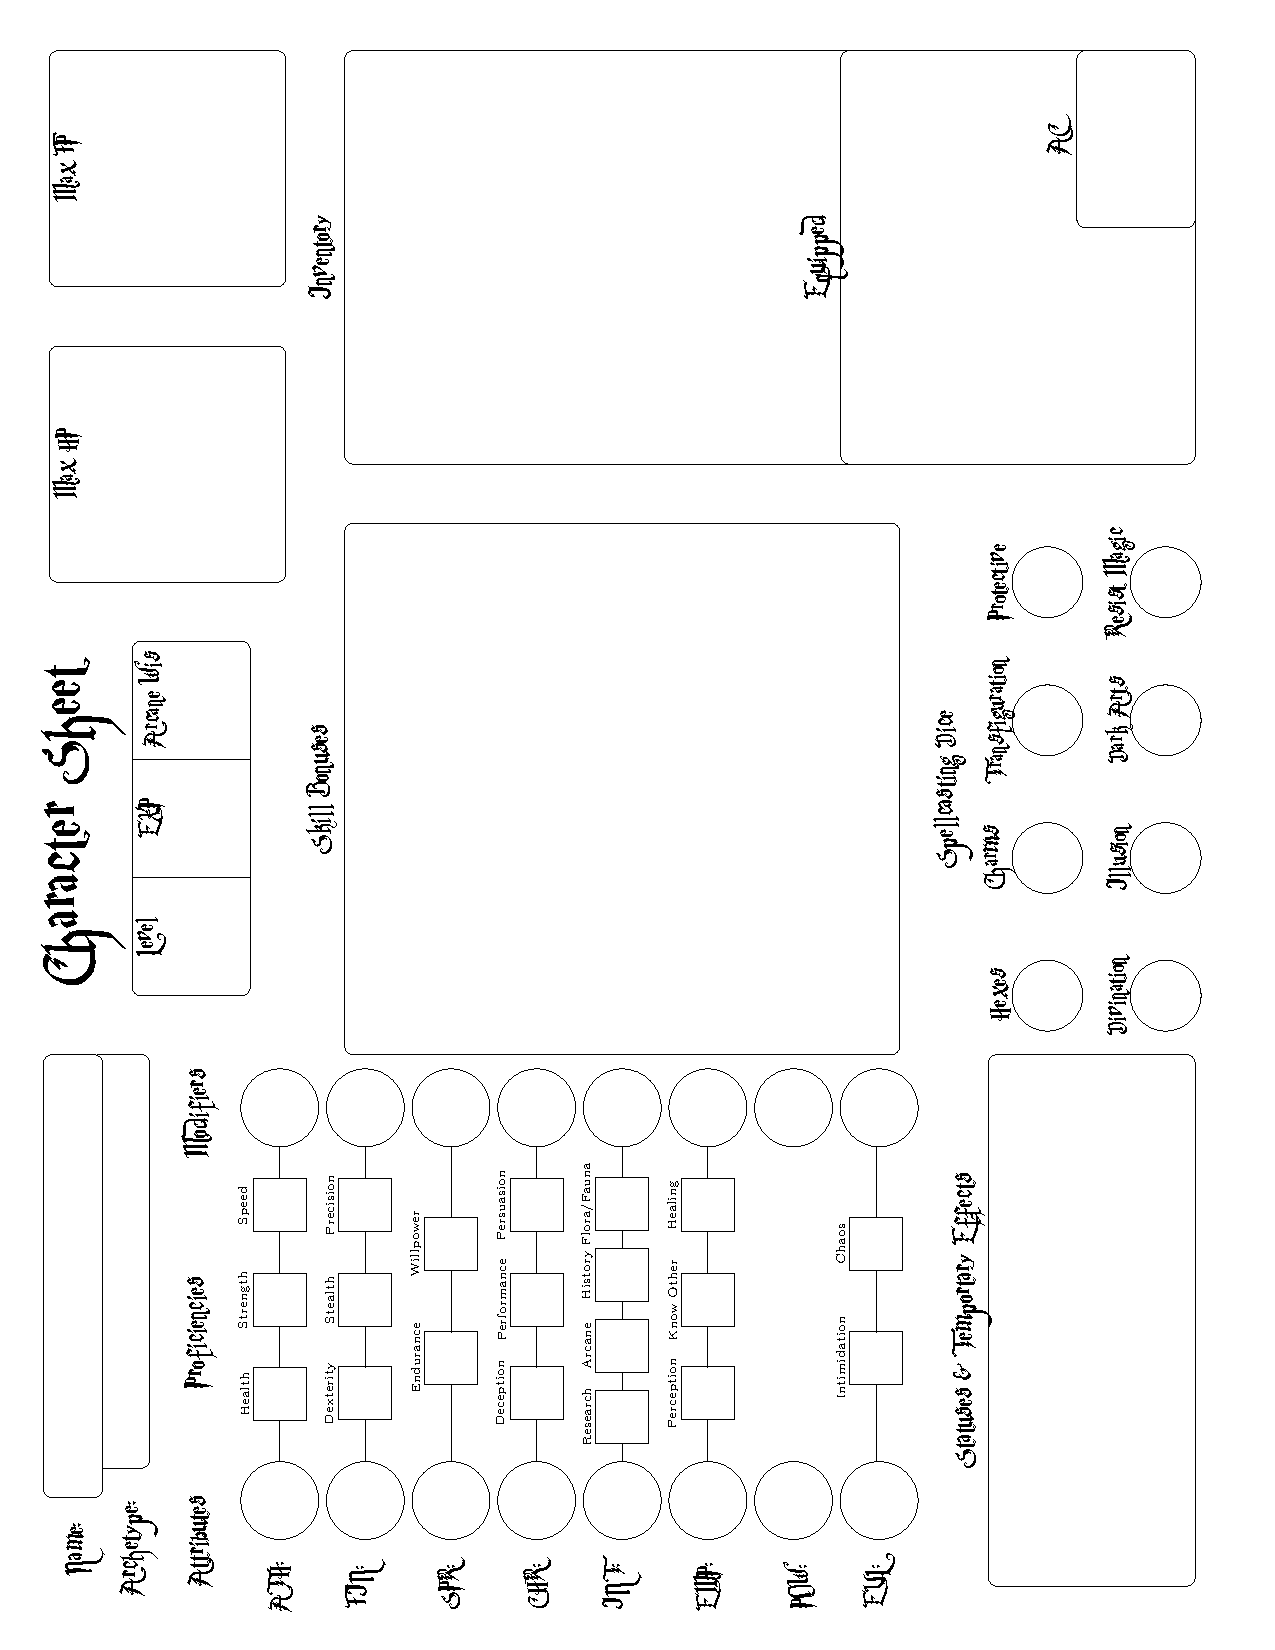
\includepdf[pages=-]{../CharacterSheet/CharacterSheet.pdf}


%\printindex
\end{document}
